% !TEX encoding = UTF-8 Unicode
\documentclass{iuphd}
\usepackage{listings}
%\usepackage[UTF8]{ctex}
\usepackage[utf8]{inputenc}
%\usepackage{xeCJK}
%\usepackage{CJKutf8}
%\setCJKmainfont{SimSun}
%\usepackage{CJKutf8}
%\usepackage[CJK,English]{babel}
%\setCJKmainfont[BoldFont=STHeiti,ItalicFont=STKaiti]{STSong}
%\setCJKsansfont[BoldFont=STHeiti]{STXihei}
%\setCJKmonofont{STFangsong}
%\usepackage{cite}
\usepackage{graphicx}
\usepackage{blindtext}
%\usepackage{showframe}
\usepackage{array}
\usepackage[export]{adjustbox}
%\usepackage[]{algorithm2e}
\usepackage[ruled,linesnumbered]{algorithm2e}
%\usepackage{algorithm}
%\usepackage[noend]{algpseudocode}
%\documentclass[UTF8,nofonts]{ctexart}
%\usepackage{pdfpages}
%\documentclass{iuphd}
%\documentclass[a4paper,12pt,times,authoryear,print,index]{iuphd}
%\usepackage[round]{natbib}
%\usepackage[font=normal,skip=0pt]{caption}
%\usepackage{natbib}
\usepackage[toc,page]{appendix}
%\usepackage{lmodern}
%\usepackage[sfdefault]{ClearSans}
\usepackage{times}
%\usepackage{tipx}
\usepackage{tipa}
%\usepackage[T1]{tipa}
\usepackage{tipx}

%\newenvironment{boxed}
%    {\begin{center}
%    \begin{tabular}{|p{0.9\textwidth}|}\includegraphics[]{dissertation.pdf}

%    \hline\\
%    }
%    { 
%    \\\\\hline
%    \end{tabular} 
%    \end{center}
%    }
%\usepackage[hebrew,english]{babel}
%\usepackage{CJKutf8}
\renewcommand*\ttdefault{cmvtt}
%\renewcommand*\familydefault{\ttdefault} %% Only if the base font of the document is to be typewriter style
\usepackage[T1]{fontenc}
%\usepackage[scaled=.83]{beramono}
%\usepackage{lipsum}
\usepackage{amsthm}
\usepackage{amsmath}
\newtheorem*{remark}{Remark}
\newtheorem{definition}{Definition}
\newtheorem{criterion}{Criterion}
\newtheorem{proposition}{Proposition}
\newtheorem{corollary}{Corollary}
\usepackage[framemethod=tikz]{mdframed}
%\DeclareFontFamily{T3}{ClearSans-LF}{}
%\DeclareFontShape{T3}{ClearSans-LF}{m}{n}
% {<-> ssub * cmss/m/n }{}
%\DeclareFontShape{T3}{ClearSans-LF}{b}{n}
% {<-> ssub * cmss/bx/n }{}
%\DeclareFontShape{T3}{ClearSans-LF}{m}{it}
% {<-> ssub * cmss/m/sl }{}
%\DeclareFontShape{T3}{ClearSans-LF}{m}{sl}
% {<-> ssub * cmss/m/sl }{}
\usepackage{natbib}
\bibliographystyle{abbrvnat}
\setcitestyle{authoryear}
%\bibliographystyle{plainnat}
%\usepackage{makecell}
% removing ACL style package
%\usepackage{styles/acl2016}
%\usepackage{palatino}
%\usepackage{tgpagella}
%\usepackage{tgschola}
%\usepackage{lmodern}
%\usepackage{tgbonum}
%\usepackage{tipa}
%\usepackage{times}
%\usepackage{latexsym}
%\aclfinaltrue
\usepackage{amsmath}
\usepackage{mathtools}
\usepackage{framed}
\usepackage{multirow}
%\usepackage{rotating}
\usepackage{subfigure}
\usepackage{wrapfig}
\usepackage{cjhebrew}
\usepackage[printonlyused,withpage]{acronym}
%\usepackage[T1, T2A]{fontenc}
%\usepackage{subcaption}
%\usepackage{dcolumn}
\usepackage{tabto}
\usepackage{url}
\usepackage{array}
\usepackage{threeparttable}
\usepackage{pbox}
\usepackage[mathscr]{eucal}
\DeclareMathOperator*{\argmax}{arg\,max}
\DeclareMathOperator*{\argmin}{arg\,min}
\usepackage{booktabs}
\newcommand\Tstrut{\rule{0pt}{2.6ex}}       % "top" strut
\newcommand\Bstrut{\rule[-1.2ex]{0pt}{0pt}} % "bottom" strut
\newcommand\TBstrut{\Tstrut\Bstrut} % top&bottom struts
%\usepackage{caption}	
%\newcommand{\myparagraph}[1]{\vspace{8pt}\noindent\textbf{#1.}}
%\newcommand{\myparagraphtwo}[1]{\vspace{8pt}\noindent\textbf{#1}\hspace{\textwidth}}
%\newcommand{\mysubparagraph}[1]{\vspace{2.5pt}\indent\textit{#1.}}
\newcommand{\itab}[1]{\hspace{0em}\rlap{#1}}
%\newcommand{\tab}[1]{\hspace{.2\textwidth}\rlap{#1}}
%\newcommand\tab[1][1cm]{\hspace*{#1}}
\usepackage{tikz}
\usetikzlibrary{positioning, calc}
\usetikzlibrary{arrows.meta}
\usetikzlibrary{shapes,arrows}
\usepackage{multicol}
\usepackage{color, colortbl}
\usepackage{gb4e}
\usepackage{etoolbox}

\makeatletter
\apptocmd{\@exe}{\singlespacing}{}{}
\makeatother

\definecolor{LightGray}{gray}{0.8}
\definecolor{LightGray2}{gray}{0.9}
%\usepackage[normalem]{ulem}
%\usepackage{nomencl}

% Uncomment this to make sure marginpars are removed before submission:
%\renewcommand{\marginpar}[1]{}
\includeonly{ch-Evaluation}

\begin{document}
%\renewcommand{\theequation}{\roman{equation}}
%\newcommand\tab[1][1cm]{\hspace*{#1}}
%\usepackage{tabto}
%data for Title Page
\title{A Multilinear Approach to the Unsupervised Learning of Morphology}
\author{Anthony Meyer}
\date{November 29, 2018}
\department{Department of Linguistics}
\maketitle
%data for Acceptance Page
%\committeechair{Committee Chair}
%\readertwo{2nd Reader}
%\readerthree{3rd Reader}
%\readerfour{4th Reader}
%\defensedate{Defense Date}
\committeeMember{Markus Dickinson, PhD (Chair)}
\committeeMember{Sandra K\"ubler, PhD}
\committeeMember{Damir Cavar, PhD}
\committeeMember{David Crandall, PhD}
\defensedate{November 29, 2018}
%data for Copyright Page
\cryear{2018}



%\makenomenclature
 
%\renewcommand{\nomname}{List of Abbreviations}
 
%\begin{document}
%\maketitle

\acceptancepage

\copyrightpage 


%\begin{dedication}
%\end{dedication}

%\begin{acknowledgments}
%The acknowledgments are designed to recognize people or agencies to whom you feel grateful for any academic,
%technical, financial, or personal aid in the preparation of your thesis or dissertation; as a matter of
%courtesy, you would ordinarily mention the members of your committee here, as well as institutions that
%provided funding, your typist, or anyone else who helped.
%I just love everyone. I just want everyone to be happy and to like me.
%\end{acknowledgments}
 
%\printnomenclature 
%\hfill % add blank space
% 
%NLP is a field of computer science, artificial intelligence, and linguistics concerned with the interactions between computers and human (natural) languages.
% 
%\nomenclature{NLP}{Natural Language Processing}
% 
%$\sigma$ is the eighteenth letter of the Greek alphabet, and carries the 's' sound. In the system of Greek numerals, it has a value of 200. 
% 
%\nomenclature{$\sigma$}{The total mass of angels per unit area}
%\begin{preface}
%\end{preface}

\begin{abstract}
This dissertation presents a multilinear approach to the unsupervised learning of morphology (ULM), where \emph{multilinear} refers to a multi-tiered architecture that allows for the handling of both concatenative and nonconcatenative phenomena in a general, unified way, as in autosegmental morphology. This dissertation reformulates autosegmental theory in graph-theoretic terms. That is, it identifies the essential properties that make autosegmental theory so conducive to modeling nonconcatenative morphology and shows that these properties are equivalent to the mathematical properties of a bipartite graph. This observation makes it possible to recast the autosegmental formalism as a graphical machine-learning model, namely the Multiple Cause Mixture Model (MCMM), a bipartite graphical model related to the Restricted Boltzmann Machine. The dissertation's experimental component consists of the development and evaluation of Multimorph, an MCMM-driven ULM system. The evaluation method takes a “dual-paradigm” approach, comprising both intrinsic and extrinsic components. The latter evaluates the system as a component of a larger chain of processes. This in line with lexeme-based theories of morphology, i.e., theories that regard morphology as a distinct but mediating layer of linguistic organization situated between phonology and syntax/semantics. The results of the experiments demonstrate the soundness and promise of a multilinear approach to the unsupervised learning of morphology.
%Outline of Current Studies Educational 

%demonstrating the fundamental equivalence between the autosegmental formalism and bipartite graphs. I
%in a machine learning system. e To motivate this approach approach presented in this dissertation distills automsegmental approach that bridges thessentially an implementation
%My primary research objective is to demonstrate \emph{how} one can 
%


%distillation of autosegmental theory as it pertains to ULM, i.e., an isolation of the fundamental properties that make it conducive to modeling non-concatenative morphology. This is accomplished by 
% I demonstrate the both the fundamental soundness of approach through both rational argument and experimental results.  f this I demonstrate the fundamental equivalence between the multi-tiered (or multilinear) architecture autosegmental theory demonstrate the relationship between bipartite graphs is approach is It is shown in this dissertation
%that This dissertation's 
%Most previous work in \ac{ULM} has treated concatenative and non-concatenative 
%morphological processes as fundamentally different, 
%e.g., by designing separate modules, one for concatenative morphology 
%and one for non-concatenative.
%This dissertation shows that an \ac{MCMM}
%can serve as a universal framework for \ac{ULM}, i.e., one that handles concatenative 
%and non-concatentive morphology in a unified manner. 
%
%My secondary research objectives address matters of implementation 
%and thus support my primary objective.
%The matters of feature-set design and the system's 
%evaluation are especially important.
%I am using exclusively word-internal features. That is, 
%there will be no 
%features referencing markings on adjacent words or any 
%other property that transcends word boundaries.
%Each feature vector (representing a word) is utterly void 
%of morphosyntactic information.
%Consequently, the \ac{MCMM} has no means of learning traditional morphemes 
%or morphosyntactic categories.
%Instead, it learns \emph{morphs}, intermediate units that reside between 
%phonology and morphosyntax. 
%However, this requires us to evaluate morphs, even though we do not know 
%beforehand what the morphs should be.
%My final research objective is thus to devise a suitable evaluation method 
%for a system that learns morphs.
%$\alpha = \rho + \sigma$
\end{abstract}
%\begin{abstract}
% The abstract is double-spaced and limited to 350 words. As many people will learn about
%your work through your abstract published in Dissertation Abstracts (http://proquest.umi.com/login),
%you should spend a good bit of effort in the composition of both the abstract and the title of your work.
%Try to convey the flavor of your work, not just the bare bones of your findings; in an average abstract
%there will be about 70 characters per line with a maximum of 35 lines. You should also work to phrase your
%title so that it truly describes the contents and will be easily found in the index of Dissertation Abstracts.
%The index is based on key words, so be as specific as you can be about your subject \cite{saund:94}.
%\end{abstract}

\tableofcontents
%\include{iuphd-doc}
\chapter*{Acronyms and Abbreviations}
\addcontentsline{toc}{chapter}{Acronyms}
\begin{acronym}[TDMA]
	\acro{1}[1p]{first person}
	\acro{2}[2p]{second person}
	\acro{3}[3p]{third person}
	\acro{n}[\textsc{n}] {\textsc{number}}
	\acro{p}[\textsc{p}] {\textsc{person}}
	\acro{g}[\textsc{g}] {\textsc{gender}}
	\acro{sg}[\textit{sg}]{singular}
	\acro{pl}[\textit{pl}]{plural}
	\acro{3ms}{third-person masculine singular}
	\acro{2ms}{second-person masculine singular}
	\acro{2fs}{second-person feminine singular}
	\acro{2mp}{second-person masculine plural}
	\acro{2fp}{second-person feminine plural}
	\acro{1cs}{first-person common-gender singular}
	\acro{1cp}{first-person common-gender plural}
	\acro{BLC}{Berman Longitudinal Corpus}
	\acro{past}[\textit{past}]{past tense}
	\acro{pres}[\textit{pres}]{present tense}
	\acro{fut}[\textit{fut}]{future tense}
	\acro{tns}[\textsc{tns}]{tense}
	\acro{perf-ptc}{perfect participle}
	\acro{MCMM}{Multiple Cause Mixture Model}
	\acro{EN}{English}
	\acro{ULM}{Unsupervised Learning of Morphology}
	\acro{MH}{Modern Hebrew}
	\acro{CH}{Classical Hebrew}
	\acro{MPS}{morphosyntactic property set}
	\acro{LPV}{Letter Predecessor Variety}
	\acro{LSV}{Letter Successor Variety}
	\acro{DM}{Distributional Morphology}
	\acro{PFM}{Paradigm Function Morphology}
	\acro{PF}{paradigm function}
	\acro{LS}{Linear Sequential}
	\acro{NLS}{Nonlinear Sequential}
	\acro{LNS}{Linear Nonsequential}
	\acro{NLNS}{Nonlinear Nonsequential}
	\acro{IPA}{International Phonetic Alphabet}
	\acro{OCR}{Optical Character Recognition}
	\acro{RBM}{Restricted Boltzmann Machine}	
\end{acronym}
\chapter{Introduction}\label{ch:intro}

%The purpose of this initial chapter will be two-fold: (1) to 
%introduce certain key concepts, such as non-concatenative morphology 
%and the unsupervised learning of morphology, 
%and (2) to state and motivate my research objectives. 
%
%\section{Preliminaries} 
%Linguists come to understand morphological 
%systems, i.e., systems of word formation, through 
%\emph{morphological analysis}, a process of isolating the fundamental units
%(traditionally, \emph{morphemes}) of which words are constructed. 
%The unsupervised learning of morphology (ULM) is the problem of devising an 
%algorithm or computational system that
%automatically induces such an analysis from raw, unannotated text.
%
%There are different categories of word-formation processes.
%One is \emph{concatenation}, whereby one morpheme is attached 
%to either the beginning or the end of another morpheme, as in the 
%English word \textit{en}$|$\textit{large}$|$\textit{s}. 
%The morphologies of many languages, including English, 
%are almost entirely concatenative. Semitic languages, however, are 
%famous for their \emph{non-concatenative} processes, whereby 
%morphemes are interleaved rather than simply concatenated.
% i.e., attached edge to edge. 

%Consider the Hebrew word 
%\textit{magdil} `he/it enlarges'. While the prefix \textit{ma-} is 
%concatenated to the stem \textit{gdil}, the stem itself is 
%non-concatenative, formed from the consonantal root \textit{g.d.l} 
%(meaning essentially `big'), and the pattern morpheme \textit{i}, meaning 
%%`cause to be \uline{\hspace{0.7cm}}'. 
%`cause to be $x$.'
%The latter is inserted 
%\textit{between} the root's second and third consonants 
%to yield a stem meaning `cause to be big' (or `enlarge').

% Explain why the unsupervised learning of \emph{non-concatenative} 
%morphology is hard: 
%Non-concatenative processes such as this one pose a particular challenge to 
%ULM. One problem is that it can 
%they imply many more ways of dividing up a word into morphemes. 
%That is, they engender many more potential (or candidate) morphemes.   
%Thus, while a few works in ULM have addressed non-concatenative 
%morphology 
%\citep[e.g.,][]{rodrigues-and-cavar:2005, botha:blunsom:13}, 
%the vast majority 
%of work has dealt solely with concatenation.
%Moreover, ULM systems tend 
%to be designed either for concatenative or for nonconcatenative morphology, 
%but generally not for both, and if they are designed  clear gap in ULM.
%The systems that do handle nonconcatenative morphology often devise different processes, one type of process to
%handle concatenative and another to handle nonconcatenative morphology.
%to be designed either for concatenative or for nonconcatenative morphology, 
%but generally not for both, and if they are designed  clear gap in ULM.

This thesis presents an approach to the unsupervised learning of morphology (ULM) that 
that marries autosegmental theory \citep{mccarthy:1981} and graphical 
computing methods. The novelty of this approach as well %as its contribution to the field 
lies in its simplicity and generality. It is equally applicable both to concatenative and 
nonconcatenative morphology, as well as to any language in theory. We will see that
autosegmental theory, once it is distilled down to its essential properties, 
connects quite naturally to graph theory, and hence to graphical approaches 
to machine learning. I will show that a bipartite graphical model in particular, 
because of its a layer of hidden nodes, exhibits the same multilinear properties 
that are behind the effectiveness of autosegmental morphology. 

%The power of autosegmental morphological theory \citep{mccarthy:1981}.
%lies in its \emph{multilinear} framework. 
%
%and adapting it for morphology. 
%has already provided a unified \emph{theoretical} 
%treatment of concatenative 
%and non-concatenative processes by taking autosegmental phonology's
%Even so, \cite{mccarthy:1981} has already provided a unified \emph{theoretical} 
%treatment of concatenative 
%and non-concatenative processes by taking autosegmental phonology's 
%\emph{multilinear} framework and adapting it for morphology. 
%A multilinear approach, illustrated in fig.~\ref{subfig:multilinear}, 
%uses multiple \emph{tiers} to represent morphological structure.
%Each morpheme occupies its own tier.
%In fig.~\ref{subfig:multilinear}, the tiers are 
%$\mu_{1}$, $\mu_{2}$, and $\mu_{3}$, which we shall call the \emph{hidden nodes}, 
%and collectively, the \emph{hidden layer}. 
%Likewise, the word itself occupies its own tier, namely the \emph{surface layer}, 
%which is composed of \emph{surface nodes} (here, the word's letters). 
%Crucially, each morpheme tier is external to the surface layer. 
%This externality allows a single morpheme, such as $\mu_{2}$ in 
%fig.~\ref{subfig:multilinear}, to connect nonadjacent surface nodes.
%However, note in fig.~\ref{subfig:linear} that when remove the external 
%morpheme tiers, we lose the capacity to unite the discontiguous \textit{gd} and \textit{l}.   
%
%The multilinear model of \cite{mccarthy:1981} has been implemented computationally i
%in non-learning systems, 
%i.e., systems driven by hand-written rules.  
%\citep[e.g.,][]{kiraz:1994, kiraz:2000}. 
%However, to my knowledge, no one has yet attempted
%to combine multi-linearity and \emph{unsupervised learning} in a single system.
%This project will seek to fill this gap.
%Moreover, because of its multilinear basis, I expect the resulting system to apply
%equally well to both concatenative and non-concatenative processes.
% \item Introduce McCarthyism. Explain how McCarthy's autosegmental 
% morphology is able to deal with non-concatenative morphology.

%\section{Autosegmental morphology}
%\label{sec:autoseg-morph}
%[Identity the property that enables it to handle discontinuous morphemes. 
%(This property is its multi-linear architecture.)]
The power and versatility of autosegmental morphological theory \citep{mccarthy:1981}
stem from its \emph{multilinear} architecture, i.e., its
%The most important component of autosegmental theory \citep{mccarthy:1981}
%is its multi-linear architecture, i.e., its
use of a \emph{segmental tier} along with many \emph{autosegmental tiers} 
to account for morphological structure. The segmental tier is
a series of placeholders for consonants and vowels, often called the
\emph{CV skeleton}. The other tiers each represent a particular \emph{morph}, i.e., unit of morphological structure.\footnote{Our choice of \emph{morph} over another term, such as \emph{morpheme}, is a deliberate  one. The question of what to call the fundamental units of morphological structure is non-trivial, since it is, practically speaking, tantamount to the question of what these fundamental units \emph{are}, i.e., what their nature is. It is thus also very pertinent to the question of what sorts of units can be induced by ULM systems. We will address these questions (as well as motivate our usage of \emph{morph}) in chapter~\ref{autonomous}.}
 
 Figure~\ref{fig:nonlinear} contrasts an autosegmental (or nonlinear) morphological analysis  with a linear one, both with respect to the Hebrew word \textit{magdil} `to make large, magnify.' 
%The autosegmental analysis for the Hebrew word \emph{magdil} `to make large, magnify.' 
In the autosegmental analysis (subfigure~\ref{subfig:nonlinear}), the morphological structure of \textit{magdil} is represented by four distinct tiers: One is the CV
skeleton, and the other three, labeled $\mu_1$, $\mu_2$, and $\mu_3$, 
correspond to morphs. Each morph is basically shorthand for a particular 
subsequence of phonemes (or graphemes). Thus, when a morph connects 
with a particular C (or V) in the segmental tier, the C (or V) inherits the 
identity one of the morph's phonemes. For example,  in 
subfigure~\ref{subfig:nonlinear}, $\mu_2$ claims the third phonological 
segment, which thus takes on the identity of  $\mu_2$'s first phoneme, 
namely /g/. The fourth phonological segment likewise belongs to $\mu_2$, 
so it manifests $\mu_2$'s second phoneme, namely /d/. Now, $\mu_2$ 
does not claim the fifth phonological segment, as it happens, and thus skips 
over it, so to speak. It does claim the sixth phonological segment, however, 
which thus becomes, in effect, $\mu_2$'s third phoneme, namely /l/. 
Note that $\mu_2$'s phonemes are mapped to phonological segments in 
order---i.e., the /g/ in $\mu_2$ is assigned before the /d/, and the C that 
is associated with /g/ must precede the C associated with /d/, etc. At the 
same, however, these \textit{C}s could be separated by any number of 
\textit{C}s or \textit{V}s, and the mapping of the morph's to phonological 
segments would still work. This is an important consequence of the nonlinear 
(autosegmental) architecture in subfigure~\ref{subfig:nonlinear}. 
%Each morph is essentially an independent data structure  both the ordering of its phonemes as well as 

%In an autosegmental framework, therefore, morphs do not depend on the particular arrangement of phonemes within the segmental string.  of phonological segments.

%morph, or units of morphological structure.
%\footnote{Even though McCarthy uses the term \emph{morpheme} rather than \emph{morphome}, the same principles apply.}

\begin{figure}[t]
%\begin{figure}{R}{0.50\textwidth}
%\vspace{-20pt}
\centering
	\subfigure[Multi-linear approach]{
	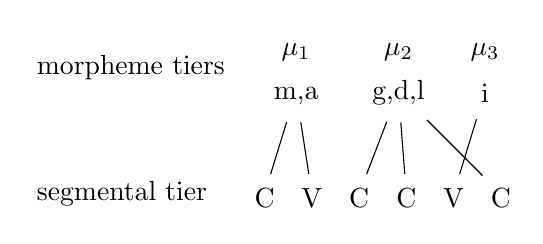
\begin{tikzpicture}[shorten >=2pt,shorten <=3pt, draw=black!100]
	\def \rowthreeht{4.4cm}
	\def \rowtwoht{3.8cm}
	\def \twopointfive{4.1cm}
	%\def \weightstwo{3.75cm}
	\def \rowoneht{2.5cm}
	%\def \weightsone{1.25cm}
	%\def \basement{2cm}
	\tikzstyle{c-node}=[text height=8pt,text centered,inner sep=3pt,minimum size=10pt]
	\tikzstyle{m-node}=[text height=7pt,text centered,inner sep=3pt,minimum size=12pt]
	\tikzstyle{r-node}=[text height=10pt,inner sep=0pt,minimum size=10pt]
	%\tikzstyle{d-node}=[text height=6pt,text centered,inner sep=0pt,minimum size=12pt]
	\tikzstyle{annot}=[text width=25ex,align=left]
	% labels
	\node[annot] (mtierstop) at (0cm,\twopointfive) {morpheme tiers};
	\node[annot] (segtier) at (0cm,\rowoneht) {segmental tier};
	%\node[annot] (mtiersbot) at (0cm,\basement) {};
	
	% surface layer
	\node[r-node] 	(r0)	at (1.0cm,\rowoneht)		{C};
	\node[r-node] 	(r1)	at (1.6cm,\rowoneht)		{V};
	\node[r-node] 	(r2)	at (2.2cm,\rowoneht)		{C};
	\node[r-node] 	(r3)	at (2.8cm,\rowoneht)	 	{C};
	\node[r-node] 	(r4)	at (3.4cm,\rowoneht)	 	{V};
	\node[r-node] 	(r5)	at (4.0cm,\rowoneht)	 	{C};
	
	% hidden-layer elements
	\node[r-node] 	(m0)	at (1.4cm,\rowthreeht)		{$\mu_{1}$};
	\node[r-node] 	(m1)	at (2.7cm,\rowthreeht)		{$\mu_{2}$};
	\node[r-node] 	(m2)	at (3.8cm,\rowthreeht)		{$\mu_{3}$};

	% hidden layer
	\node[c-node] 	(m3)	at (1.4cm,\rowtwoht)		{\/m,a\/};
	\node[c-node] 	(m4)	at (2.7cm,\rowtwoht)		{\/g,d,l\/};
	\node[c-node] 	(m5)	at (3.8cm,\rowtwoht)		{\/i\/};
		
	\path
		(m3)	edge	node	{}	(r0)
		(m3)	edge	node	{}	(r1)
		%
		(m4)	edge	node	{}	(r2)
		(m4)	edge	node	{}	(r3)
		(m4)	edge	node	{}	(r5)
		%
		(m5)	edge	node	{}	(r4);
		
	\end{tikzpicture}
	\label{subfig:nonlinear}
	}

	\subfigure[Linear approach]{
	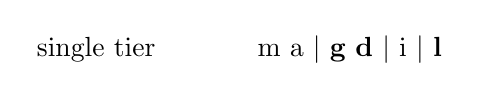
\begin{tikzpicture}[shorten >=1pt,draw=black!100]
	\vspace{50pt}
	\def \floor{0cm}
	\tikzstyle{f-node}=[text centered,inner sep=0pt] %text centered]
	\tikzstyle{annot}=[text width=34ex,align=left]
	% labels
	\node[annot] (floorlabel) at (0cm,\floor) {single tier};
	
	% surface layer
	\node[f-node] 	(f0)	at (1.4cm,\floor)			{m\,\,a\,\,$|$\,\,\textbf{g}\,\,\textbf{d}\,\,$|$\,\,i\,\,$|$\,\,\textbf{l}};
	\end{tikzpicture}
\label{subfig:linear}
}
\label{fig:nonlinear}
\caption{Multiple tiers vs. a single tier}
%\vspace{-20pt}
%\vspace{1pt}
\end{figure}

%Notice that $\mu_2$, the consonantal root, is discontinuous; it is
%interrupted by $\mu_3$. 
%This autosegmental account of the 
By contrast, the analysis in subfigure~\ref{subfig:linear} is the \emph{linear} counterpart to the autosegmental  (or nonlinear) analysis in fig.~\ref{subfig:nonlinear}
If a model should have only one tier, as in 
fig.~\ref{subfig:linear}, there would be no way of representing the
unity of $\mu_2$, i.e., the fact that \textit{g}, \textit{d}, and \textit{l}
all belong to the same morphological unit. Observations such these motivate this thesis's two principal concepts: \emph{nonlinearity} and \emph{nonsequentiality}. We will define these concepts now and revisit them further in subsequent chapters. 

	\begin{definition}\label{def:nl}{\textsc{Nonlinearity}}: %A model is \emph{nonlinear} 
	A model is \textbf{nonlinear} if each of its morphs occupies a tier that is \emph{not} the phonological tier.
	%Morphs, i.e., units of morphological structure, must be separate from the surface (or phonological) tier. \end{definition} %, i.e., as residing on tiers distinct from the phonological tier. %eparately for m  as being separate from (or outside of) the the phonological (or segmental) tier.  % is a property wherein morphs are represented as being separate from the segmental tier.
	\end{definition}
	\begin{definition}\label{def:ns}{\textsc{Nonsequentiality}}: %is a property such that each morph tier (or node) is orthogonal to all other morph tiers.
	%---i.e., independent of---all other morph tiers. 
	A model is \textbf{nonsequential} if \textbf{no two morphs} occupy the \emph{same} tier. This is to say that all morphs are independent, i.e., that there are no morph-to-morph connections.
	\end{definition}
I propose that these two properties are the essential properties that enable autosegmental morphology to handle nonconcatenative morphology. The main idea of this thesis is that these two properties must be present in any model in order for it to be capable of handling (or learning) nonconcatenative morphology.  We will also revisit this idea later (see in particular section~\ref{sec:framework-intro}).
\begin{proposition}\label{prop:nlns}
A model of morphology can handle nonconcatenative morphology if and only if it satisfies both \textbf{nonlinearity} and \textbf{nonsequentiality}. %  the modeling of nonconcatenative morphology.}
\end{proposition}
%\pex~ Two essential properties  %\ex \label{ex:properties}\begin{xlist}
%	\a {\textsc{Nonlinearity}}: Morphemes are represented as being separate from the segmental tier.
%	\a {\textsc{Nonsequentiality}}: Each morpheme tier (or node) is orthogonal to---i.e., independent of---all other morpheme tiers.
%\xe
% \ex this is one 
%\marginpar{or multilinear}
%These criteria, or essential properties,
%%\textsc{nonlinear} and \textsc{nonsequential} 
%are basically binary variables; each \emph{must} be either True or False, and each can \emph{only} be True or False.  Each variable thus has two possible values,
%giving us four possible combinations of (non)linearity and (non)sequentiality: 
%\textbf{nonlinear nonsequential} (NLNS), \textbf{linear nonsequential} (LNS), 
%\textbf{nonlinear sequential} (NLS), and \textbf{linear sequential} (LS).

%[We should note that autosegmental morphology has other properties to
%constrain morphological structure, e.g., the well-formedness
%principle; at present, we are not concerned with capturing all aspects
%of autosegmental morphology, but instead in building a generic system
%to which one can later add linguistically motivated constraints.]

\section{Research Questions and Objectives}
%State primary research objective: 
%\subsection{Primary research objective}
The primary objective of this thesis is to demonstrate the idea expressed above as proposition \ref{prop:nlns} through a combination of rational argument and experimentation.
%that the crucial components of autosegmental theory, i.e., 
%those components that allow it to handle non-concatenative morphology, 
%This will be accomplished both through rational argument and experimentation.
The rational argument will consist in three main points.
First, the properties of nonlinearity and nonsequentiality are absolutely essential for dealing with nonconcatenative morphology.
Second, these properties are equivalent to the formal mathematical properties that define bipartite graphs. And third, this equivalence provides a foundation for the use of graphical learning models for the purpose of morphological learning. 
%The present study uses a graphical learning framework known as the Multiple Cause Mixture Model (MCMM) \citep{saund:94}. 
These points will be further fleshed out in chapters \ref{ch:lit-review}, \ref{ch:graph}, and\ref{ch:MCMM}. 
The experimental component of the dissertation consists of the development and evaluation of
 \textbf{Multimorph}, a novel unsupervised morphology-learning system that is driven by an MCMM and embodies the three points stated above.
%The input data consisted of Modern Hebrew words represented as feature vectors. 
%The present study focuses on the learning of Modern Hebrew, since Modern Hebrew
%exhibits both concatenative and non-concatenative morphological processes 
%and thus provides a good test of the method's generality.
%\subsection{Secondary research objectives}
%\label{sec:secondary-objectives}
%My secondary research objectives are outlined below. %They are largely concerned with matters of implementation. 
	
	 \subsection{The Question of Features} There is a great deal of information tacitly present in a string of alphabetic symbols.
	 This is true regardless of whether the string is written, in which case the symbols are graphemes, or spoken,
	 in which case they are phonemes. In either case, the symbols are each drawn from an alphabet of size $N$ and arranged along a single axis. % (say, the $x$ axis).
%Consider the string of graphemes printed below.
By way of illustration, consider again the Hebrew word \textit{magdil}, but now specifically as a \emph{string of graphemes}: 
%from figure~\ref{fig:nonlinear}, but now we think of it specifically as the \emph{string of graphemes}.
\begin{figure}[h]
\vspace{12pt}
	\centering
	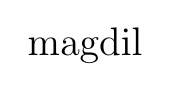
\begin{tikzpicture}[shorten >=2pt,shorten <=3pt, draw=black!100]
	\Large
	\def \rowoneht{0cm}
	\def \rowtwoht{-0.8cm}
	\tikzstyle{r-node}=[text height=10pt,inner sep=0pt,minimum size=10pt]
	%\node[r-node] 	(r0)	at (0cm,\rowoneht)		{\textipa{magdil}};
	\node[r-node] 	(r0)	at (0cm,\rowoneht)		{magdil};
	%\node[r-node] 	(r0)	at (0cm,\rowoneht)		{s t o p};
	%\node[r-node] 	(r0)	at (0cm,\rowtwoht)		{p o t s};
	\end{tikzpicture}
\end{figure} \\
%This row of six graphemes contains a vast amount of tacit information. For instance, suppose we had to represent the string \textit{magdil} not as sequence of alphabetic symbols, but as a series of simple declarative statements. We might come up with statements like the following: 
%%These statements might say that a certain character is present in the string, that one character precedes another character, that a particular character occurs at a particular position in the string, and so on, as in the following examples.
%\begin{itemize}
%  \item \textit{a} immediately follows \textit{m}, \textit{g} immediately follows \textit{a}, \textit{d} immediately follows \textit{g}, and so on. 
%  \item \textit{i} immediately precedes \textit{l}, \textit{d} immediately precedes \textit{i}, and so on.
%     \item \textit{g} follows both \textit{m} and \textit{a}, \textit{d} follows \textit{m}, \textit{a}, and 
%   \textit{g}; \textit{d} precedes both \textit{i} and \textit{l}, \textit{g} precedes \textit{d}, \textit{i}, and \textit{l}, and so on.
%   \item \textit{m} is the first character, \textit{a} is the second, \dots \textit{i} is the second-to-last character, and \textit{l} is the last character, and so on.
%   %\item \textit{l} is the sixth character, \textit{i} is the fifth, \textit{d} is the fourth, and so on.
%   \item \textit{m} precedes \textit{a}, \textit{m} precedes \textit{g}, \textit{m} precedes \textit{d}, \dots, \textit{m} precedes \textit{l}; \textit{a} precedes \textit{g}, \dots , \textit{a} precedes \textit{l}; and so on.
%   \item \textit{m} is present, \textit{a} is present, \textit{g} is present, and so on.
%   \item \emph{ad infinitum}
%\end{itemize}
%A string of alphabetic symbols tacitly conveys all of these facts and many more---perhaps infinitely more.
%Statements like these are essentially what we call \emph{features}.
%Each statement can be either true or false, which is to say that each feature is \emph{binary}, drawn from an alphabet of size $N = 2$.  
%Many machine learning models require that each input object or \emph{learning instance} (in our case, each \emph{word}) be represented as a vector of binary features, not alphabetic features. Moreover, all input objects (learning instances) must be described by the same feature set, and all feature vectors must be of the same length.
%One cannot, of course, have an infinite number of features, as feature vectors must be finite in length.
%Now, let $F$ be the infinite set of all possible features. In keeping with the spirit of my primary research objective, we shall assume that there exists at least one $\phi$ such that $\phi \subset F$, $\phi$ is finite, and $\phi$ allows a ULM system to learn a multilinear model of morphology. The objective here is to confirm this assumption, i.e., to find such a subset.
%There is a great deal of information tacitly present in a string of alphabetic symbols.
%This is true regardless of whether the string is written, in which case the symbols 
%are graphemes, or spoken, in which case they are phonemes. In either case, 
%the symbols are each drawn from an alphabet of size $N$ and arranged along 
%a single axis. % (say, the $x$ axis).
%By way of illustration, consider again the Hebrew word \textit{magdil}, but now specifically as a \emph{string of graphemes}.  In  
%from figure~\ref{fig:nonlinear}, but now we think of it specifically as the \emph{string of graphemes} 
%printed at the top of figure~\ref{fig:many-feats}. 
%By way of illustration, consider the string of graphemes
%displayed at the top of figure~\ref{fig:many-feats}.
%\begin{figure}[h]
%	\centering
%	\begin{tikzpicture}[shorten >=2pt,shorten <=3pt, draw=black!100]
%	\Large
%	\def \rowoneht{0cm}
%	\def \rowtwoht{-0.8cm}
%	\tikzstyle{r-node}=[text height=10pt,inner sep=0pt,minimum size=10pt]
%	%\node[r-node] 	(r0)	at (0cm,\rowoneht)		{\textipa{magdil}};
%	\node[r-node] 	(r0)	at (0cm,\rowoneht)		{magdil};
%	%\node[r-node] 	(r0)	at (0cm,\rowoneht)		{s t o p};
%	%\node[r-node] 	(r0)	at (0cm,\rowtwoht)		{p o t s};
%	\end{tikzpicture}
%\end{figure}
This six-grapheme string contains a vast amount of tacit information. For instance, 
suppose we had to represent the string \textit{magdil} not as sequence of alphabetic 
symbols, but as a series of simple declarative statements. We might come up with 
statements like the following: 
%in in figure~\ref{fig:many-feats}
%\begin{figure}[h]
%%line\hline
%%These statements might say that a certain character is present in the string, that one character precedes another character, that a particular character occurs at a particular position in the string, and so on, as in the following examples.
%\begin{center}
%\Large{magdil}
%\end{center}
%%\smallskip
\begin{itemize}
  \item \textit{a} immediately follows \textit{m}, \textit{g} immediately follows \textit{a}, \textit{d} immediately follows \textit{g}, and so on. 
  \item \textit{i} immediately precedes \textit{l}, \textit{d} immediately precedes \textit{i}, and so on. %What's more, we know that
   \item \textit{g} follows both \textit{m} and \textit{a}, \textit{d} follows \textit{m}, \textit{a}, and \textit{g}; \textit{d} precedes both \textit{i} and \textit{l}, \textit{g} precedes \textit{d}, \textit{i}, and \textit{l}, and so on.
   \item \textit{m} is the first character, \textit{a} is the second, \dots \textit{i} is the second-to-last character, and \textit{l} is the last character, and so on.
   %\item \textit{l} is the sixth character, \textit{i} is the fifth, \textit{d} is the fourth, and so on.
   \item \textit{m} precedes \textit{a}, \textit{m} precedes \textit{g}, \textit{m} precedes \textit{d}, \dots, \textit{m} precedes \textit{l}; \textit{a} precedes \textit{g}, \dots , \textit{a} precedes \textit{l}; and so on.
   \item \textit{m} is present, \textit{a} is present, \textit{g} is present, and so on.
   \item \emph{and so on \dots}
\end{itemize}
%\hline
%\end{tikzpicture}
%\caption{Innumerable possible features.}
%\begin{tikzpicture}
%\label{fig:many-feats}
%\end{figure}
%A string like \textit{magdil} tacitly conveys all of these facts and many more---perhaps 
%infinitely more. 
All of these statements, as well as many others,
are tacitly expressed in the string \textit{magdil}.

What we call \emph{features} are essentially true-or-false statements like those listed above.
% ones in figure~\ref{fig:many-feats}.
%Each statement can be either true or false, which is to say that each feature is \emph{binary}, 
%drawn from an alphabet of size $N = 2$.  
Many machine learning models require that each input object or \emph{learning instance} 
(in our case, each \emph{word}) be represented as a vector of binary features, not alphabetic 
features. Moreover, all input objects (learning instances) must be described by the same feature 
set, and all feature vectors must be of the same length.
One cannot, of course, have an infinite number of features, since feature vectors must have a definite length.
One must therefore choose a particular subset of all possible features. The problem of choosing a likely subset constitutes one of
this dissertation's main research questions, and we
%In \ref{ch:intro}, we mentioned the problem of choosing one finite subset of features from an infinite number of possible features.
address it further in chapter~\ref{ch:experi}, where we will glean some insight 
by considering feature categories that 
are significant to computer vision, particularly \emph{invariant} and \emph{variant} features. I will argue that the distinction between these two categories is also important to the unsupervised learning of morphology.
% with an eye to better understanding the sort of features that are valuable to the unsupervised learning of morphology. 
%The idea is that 
%the task of clustering objects, i.e., discerning what makes two objects similar and what makes them different,
%and figuring out which objects to group together and which to separate, is a very general problem. And thus the
%same types of features should apply to different types of objects.
%These categories are \textit{variant} features and \textit{invariant} features. 
%>>>
%We will focus in particular on \emph{invariant} and \emph{variant} features. The distinction between these two categories is highly significant in
%computer vision and its various subfields. For the purposes of this dissertation, we hypothesize that this distinction is
%also important to unsupervised morphological learning. 


\subsection{The Question of Data Representation} 
 %emph{representation} of the input data,
In extracting features from the original data, i.e., a list of words, one is of altering the dataset. Different feature categories emphasize different kinds of information. But the raw material for feature extraction is any case the original word list, and thus the way in which the words represented in the original dataset plays its own role in shaping features. 
By \emph{representation}, we refer mainly to the alphabet---the
particular set of symbols---from which the strings (i.e., words) of the input wordlist 
are composed.  A word is fundamentally something spoken, i.e., a sequence of sounds, and thus in order to write the word down, one must devise a way to represent the spoken phenomenon on paper. Like feature-set design, this is a means of emphasizing some information at the expense of other information. All else being equal---i.e., even if the feature categories are the same---different modes of data representation will produce different features.  
In the present work, three manners of data representations were tested, each presenting 
different information. 

The question of how the input data should be represented is an important one in morphological learning because there are often 
a variety ways to represent linguistic data in text form. 
For instance, Japanese can be written in written in \textit{kanji} or 
\textit{kana} characters. The former are entirely logographic, as they 
have been borrowed directly from the Chinese \textit{Han} script, 
and as such, they are not connected to speech sounds in any way. The latter, by contrast,
represent syllables of spoken Japanese. That is, each single \textit{kana} 
character represents both a consonant and a vowel.  (Japanese syllables consist of a consonant onset and a vowel nucleus.)  Japanese can also be represented via alphabetic systems, which including several systems of Romanization as well as scientific phonetic transcription systems such as the International Phonetic Alphabet (IPA).  One might reasonably ask how these various ways of representing Japanese as text might influence the unsupervised learning of Japanese morphology.

%There are indefinitely many ways to represent any language. 
%combination of this two. \textit{Kanji} are logographic characters borrowed directly from the Chinese \texit{Han} script, whereas \textit tAs logographic characters, they are not connected to speech sounds. Japananese   characters and ar chaSome modes of representation 
%are more transcriptional, 
%and others lean toward the orthographic. Some might go to great lengths to capture every phonological and morphophonemic alternation, while others might not express 
%any alternations. Still others might express graphemic alterations; for example, 
%some scripts have different shapes for some letters when the occur word-finally. 
%Some scripts might represent some phonological alternations, but not others, 
%perhaps because those alternations are perceived as more salient than others.
Like that of Japanese, the orthography of Hebrew has a long and rich history. Unlike Japanese, however, Hebrew has never been represented in a non-alphabetic script. Indeed, the ancient Hebrew alphabet was essentially the Phoenician alphabet, the world's first alphabetic writing system and the progenitor of all the alphabets that would in emerge in Europe and the Near East. Still, Hebrew orthography is by no means a straightforward matter, as we shall see in chapter~\ref{ch:experi}.
This dissertation tests three different modes of representing Hebrew as text:
\begin{enumerate}
\item Transcriptions that mark the primary stress in words
\item Transcriptions without stress markings 
\item Standard Hebrew orthography 
\end{enumerate} 
The third category---the standard orthography---is significant because standard Hebrew 
orthography lacks symbols reserved for vowels. Its alphabet consists only of consonants.\footnote{Some consonants can be used to represent vowels, namely the Hebrew equivalents of \textit{w} (pronounced as [v] in Modern Hebrew), \textit{y}, and \textit{h}. Even so, these symbols are still fundamentally consonants. This and other matters of Hebrew orthography will be discussed in chapter~\ref{ch:experi}.}

I initially hypothesized that models induced from the orthographic 
data would produce the worst-performing models. The reasoning behind this 
hypothesis was that, first, any system that lacks vowels has 
to be information- deficient, and second, vowels must be particularly important to 
Hebrew because its derivational morphology consists of interleaving consonantal 
roots and vowel patterns. The results, however, proved to be somewhat surprising, 
as we shall see in chapter~\ref{ch:results}.
% morphology consist missing out on a great deal of valuable information  It seemed that a vowel-less spelling system would since it seems so obvious that by lacking vowels, it is lacking set wi particularly note this study is noteworthy because the Hebrew alphabet has no vowelsinv take on a different shape word-finally. to a great   to a greater e  The question of data representation determines the raw material from which features are constructed, touches on a number concern the role of the input data in morphological learning, the distinction between information quantity and quality in the input data, as well the influence of 

%transcriptional representations. These differed only in that one marked stress and the other did not. (i.e., all vowels of the t (TS and TR, respectively); The third was \emph{orthographic}, comprising 
%the letters of the standard Hebrew alphabet mapped onto ASCII characters.
%%(\textbf{\text{T}^{S}); another transcriptional, but without stress (\textbf{\text{T}^{R}), and the third orthographic (\textbf{O})ransliterated to ASCII characters in the Hebrew Treebank \citep{simaan-et-al:2001}
%TS is the Berman Longitudinal Corpus's transcriptional system, 
%and TS is that same system with the stress markings removed. 
%%Its alphabet is thus BLC's 
%%transcriptional system, which we discussed above in section. % \ref{sec:transcription}.
%The information contained in O is differs both qualitatively and quantitatively from information contained in the T datasets  
%Arguably, T contains more information than O,
%since T represents each of Modern Hebrew's five vowels in such a way that each 
%vowel sound not only has a symbol, but its own
%has its own exclusive symbol 
%exclusive symbol.

%The features are extracted from raw-text data, wherein Hebrew words are represented as strings of alphabetic symbols, and the symbols are drawn from a particular alphabet. Now, it so happens that we have more than one alphabet at our disposal, and thus more than one way to represent the input data. These alphabets are the following:
%	\begin{enumerate}
%		\item \textbf{Modern Hebrew standard orthography}, as transliterated to ASCII characters in the Hebrew Treebank \citep{simaan-et-al:2001}. In the orthography of Modern Hebrew, certain consonants are regularly appropriated to represent vowels. For example, the Hebrew letter
%		\textcjheb{w}, transliterated as \textit{w} in the Hebrew Treebank, is by default the consonant /v/, but it is also used to represent the vowels /o/ and /u/. In most syllables, however, the vowel is not represented at all. 
%		\item \textbf{Phonemic transcriptions}, i.e., phonemically transcribed words. I have extracted two lists of phonemically transcribed words from the Hebrew portion of the CHILDES database \citep{macwhinney:2000a}. 
%		 These lists are the same except that stress is marked in one, but not in the other.
%	\end{enumerate}
%	%The phonemic transcriptions amount to 12,494 words.
%	The question is which mode of representation yields better feature vectors. This is equivalent to asking which mode delivers the largest quantity of useful information and/or the smallest quantity of irrelevant information.
%	\paragraph{Mixing and Objective Functions.} The \textbf{mixing function} 
%is essentially a voting rule \citep{saund:94}. It prescribes the method whereby the 
%``votes'' of  hidden units are combined to turn a particular feature (i.e., surface unit) \textsc{on} or \textsc{off} (see section~\ref{sec:mixing-function}. The \textbf{objective function} measures the discrepancy---or, alternatively, similarity---between the surface units' activities and their target activities. 
%It thus drives the model's learning by way of trial and error. Objective functions can 
%be either positive or negative. Positive objective functions measure similarity and thus 
%need to be maximized. Negative objective functions measure error and thus need to be minimized (see section~\ref{sec:mcmm-learning}).

%I intend to experimented with two radically different mixing functions, 
%viz. one that combines hidden-unit activities linearly and one that combines them nonlinearly.
%%%(see section~\ref{sec:mixing-function}). 
%Similarly, I intend to try out 
%two radically different objective functions, namely 
%both a negative and a positive % one (see section~\ref{sec:mcmm-learning}).
%objective function. %(see section~\ref{sec:mcmm-learning}).
%Why: What does the mixing function do? What would happen if there were no mixing function? The mixing function maps the hidden-unit activities
%What does the objective function do? What would happen if there were no objective function? 
%If there were no objective function, there could be no learning. Learning proceeds by trial and error. 
%The objective function supplies the error.

\subsection{The Problem of Evaluation}  One goal of unsupervised learning is to discover previously unknown categories \citep{parsons:2004}. This is especially true where the present study is concerned. Chapter~\ref{autonomous} argues that unsupervised morphological learners by nature learn \emph{autonomous} morphological units, i.e., units that reside in an independent between phonology and syntax. Such units have no meaning in and of themselves, as they exist independently of syntax and semantics. It is difficult to know going into an experiment what these categories should look like, i.e., what would make such units of intermediate structure correct or incorrect. 

%going
%The previously unknown categories in this case are going to be morphological units of some kind.
%However, these units will not be conventional morphemes or morphosyntactic categories. 
%
%Instead, MCMM-generated clusters will correspond roughly to Aronoff's 
%\emph{morphomes} \citep{aronoff:1994}, which can be described as \emph{pre-morphosyntactic} units, i.e.,
%units that have been assembled from phonemes, but have not yet been assigned 
%a syntactic or semantic meaning. I shall use the term \emph{morph} instead of 
%\emph{morphome}, however, since MCMM-generated clusters may not correspond 
%precisely to morphomes in every case (see section~\ref{sec:targets}).

Thus, the evaluation itself presents an important research question, namely the question of how to evaluate the output of an unsupervised morphological clustering algorithm, particularly one that considers only features of \emph{word-internal form}, having no access to word-external morphosyntactic features, e.g., the person, number, and gender of surrounding words. 

%Thus, my system will not require morphological building blocks to have particular
%meanings. Instead, it 
%My system will thus look for \emph{pre-morphosyntactic} 
%units, i.e., ones assembled from phonemes, but not yet assigned 
%a syntactic or semantic meaning. In a larger pipeline, such 
%building blocks could serve as an interface between morphosyntax 
%and phonology. For instance, while an MCMM can find Hebrew's default 
%masculine suffix \textit{-im}, it cannot say whether it is
%masculine or feminine in a given word, as this suffix
%also occurs in idiosyncratic feminine plurals. The extrinsic part of the evaluation will examine my system's utility as a component within such a pipeline
%(see section~\ref{sec:paradigms}).
%\emph{morphs}. \marginpar{I have yet to introduce morphs, tho} We do not know 
%beforehand \emph{exactly} what these morphs ought to look like. Since we cannot know 
%the ``right answers'' before the experiments are run, there can be no clear gold 
%standard against which to evaluate the MCMM's output. 
%
%Thus, the evaluation itself presents an important research question, namely the question of how to evaluate the output of an unsupervised morphological clustering algorithm, particularly one that considers only features of \emph{word-internal form}, having no access to word-external morphosyntactic features, e.g., the person, number, and gender of  surrounding words. Such an algorithm will inevitably produce clusters that do not correspond to abstract morphosyntactic categories or conventional morphemes.
%which are fundamentally morphosyntactic in nature even though the correspondence between morphemes and abstract, or ``atomic,'' morphosyntactic categories is not always one-to-one.

\section{Organization}
The remainder of this thesis is organized as follows: In chapter~\ref{ch:lit-review}, I present a new framework for thinking about the unsupervised learning of morphology. This framework is original to this thesis and stems from the concepts of nonsequentiality and nonlinearity, introduced above as the essential prerequisites for modeling nonconcatenative morphology. Chapter~\ref{ch:graph} establishes the relationship between autosegmental morphology and graph theory, particularly \emph{bipartite} graphs. Chapter~\ref{ch:MCMM} then introduces and describes a particular bipartite graphical learning model, namely the Multiple Cause Mixture Model (MCMM). As mentioned above, this is the learning model I have chosen to drive Multimorph, the system developed in this dissertation. The first four chapters thus establish a logical chain linking autosegmental morphological theory to a particular unsupervised learning model, namely the MCMM, which serves Multimorph's learning model. 

The remaining five chapters (chapters \ref{autonomous} through \ref{ch:conclusion}) are concerned with the evaluation of Multimorph. Chapter~\ref{autonomous} addresses the question of the sort of categories that Multimorph and other unsupervised morphological should be expected to learn, i.e., the sort of categories that one should look for in evaluating such systems. This is part of the ``question of evaluation'' introduced above. Chapter~\ref{ch:experi} describes the experimental setup; i.e., it describes the collection and preparation of the datasets and the experimental variables, including the three modes of data representation and the parameters for the feature sets. Chapter~\ref{ch:eval} completes this thesis's response to the ``question of evaluation.'' It describes a dual-paradigm evaluation method consisting of both an intrinsic and extrinsic component. The extrinsic component in particular may be of interest to other ULM researchers as an alternative to conventional evaluation methods. Finally, chapter~\ref{ch:conclusion} offers concluding remarks. 
\chapter{A CONCEPTUAL FRAMEWORK FOR UNSUPERVISED MORPHOLOGICAL LEARNING}
\label{ch:lit-review}

\section{Introduction}
\label{sec:framework-intro}
\cite{mccarthy:1981} points out a fundamental flaw in linear, 
concatenative approaches to morphological analysis: 
Such approaches acknowledge only a single level of representation, 
namely that of the \emph{segmental string}, i.e., the level of minimal 
phonological segments (essentially phonemes).\footnote{McCarthy uses
 the term \emph{segment} in the phonological sense, i.e., a minimal unit of sound. 
Researchers in \ac{ULM}, however, generally use the word to 
refer to minimal morphological units, 
as in \textit{the problem of morphological segmentation}, for example.}  \marginpar{Strange footnote.}
Because they are restricted to this single layer, they can only represent 
morphological groupings in one way, namely to insert delimiters of 
some sort 
into the very string under analysis. At any given
insertion point, moreover, such an approach can see only the two segments 
(i.e., phonological segments) immediately to the left and right. It thus
has no way to identify morphs that are made up of discontiguous phonemes.

\cite{mccarthy:1981} offers an alternative \emph{nonlinear} 
approach to grouping segments into morphs, one that liberates the 
representation of morphs from the segmental tier. McCarthy's formalism, 
\\emph{autosegmental morphology}, is an extension of the autosegmental 
approach to phonology developed by \citep{goldsmith:1976} to account 
for nonlinear phonological phenomena. One such phenomenon, for instance, 
is \emph{tone spreading}, whereby the tone on one vowel spreads to other 
vowels, leapfrogging any intervening consonants. 
Goldsmith's solution was to introduce \emph{autosegmental} tiers 
(or planes) of representation that were independent of and external 
to the segmental tier---tiers that could thus ``see'' and access any 
phonological segment in the segmental tier, as well as any subsequence 
of segments, contiguous or discontiguous. The key was the nonlinearity 
(or multilinearity)\footnote{The terms \emph{nonlinear} and \emph{multilinear} 
interchangeably in this work, as they both mean, essentially, ``not linear."}
introduced by the multiple tiers and their separation both from each other 
and the segmental tier. 
McCarthy's insight was that this same nonlinear architecture could be 
applied to the problem of nonconcatenative morphology, particularly the 
root-and-pattern morphology of Semitic languages. 

I have cooked up my own novel framework for comparing (and classifying)
previous approaches
the unsupervised learning of morphology. This framework is a classification 
system derived from the definitions of nonlinearity and nonsequentiality 
(see chapter~\ref{ch:intro}, definitions \ref{def:ns} and \ref{def:nl}) 
and the proposition that 
a model can learn nonconcatenative morphology if and only if it 
possesses both of these categories (chapter~\ref{ch:intro}, 
proposition~\ref{prop:nlns}). In particular, first observe that nonlinearity 
and nonsequentiality are negative concepts and thus suggest the existence 
of their ``positive'' counterparts, namely \emph{linearity} and 
\emph{sequentiality}. To facilitate the exposition of these concepts, we 
repeat the definitions of nonlinearity and nonsequentiality here and 
then define their complements, \emph{linearity} and \emph{sequentiality}.
	\begin{description}%\label{def:nl}
	%\begin{definition*}
	%\item[{\textsc{Nonlinearity}}:]A model is 
	\item[\textbf{nonlinear}] if each of its morphs occupies a tier that is \emph{not} the phonological tier.
	%\end{definition*}
	%\begin{definition*}
	%\label{def:ns}
	\item[{\textsc{Nonsequentiality}}:]
	A model is \textbf{nonsequential} if \textbf{no two morphs} occupy the \emph{same} tier. This is to say that all morphs are independent, i.e., that there are no morph-to-morph connections. 
	\end{description}
	\begin{definition}\label{def:l}{\textsc{Linearity}}:
	A model is \textbf{linear} if (at least some of) its morphs occupy the phonological tier.
	\end{definition}
	\begin{definition}\label{def:s}{\textsc{Sequentiality}}:
A model is \textbf{sequential} if (two or more) morphs occupy the \emph{same} tier.\footnote{In practice, `` two or more morphs'' is tantamount to saying ``all morphs,'' since it is hard to envision a scenario in which only a subset of morphs occupy separate tiers.}. This is to say that there are connections between at least some pairs of morphs.
	\end{definition}

Proposition \ref{prop:nlns} asserts that \emph{both} nonlinearity \emph{and} nonsequentiality
must be present in a model if it is to capable of modeling nonconcatenative morphology.
 In other words, the category of models capable of the learning nonconcatenative 
 morphology is  the intersection of the (more general) nonlinear and 
 sequential categories. Thus, one of our framework's categories has to be 
 \textbf{nonlinear-nonsequential}. Indeed, this is the ``desired'' category, 
 so to speak, the category whose members are intrinsically capable of modeling/learning
 nonconcatenative morphology. The other three are likewise each the intersections 
 of two of the basic categories outlined above.  For instance, another category is \textbf{nonlinear-sequential}, 
 or the intersection of the nonlinear and sequential categories. The remaining two categories, 
 \textbf{linear-nonsequential} and \textbf{linear-sequential} are analogously defined. The four categories are summarized in figure~\ref{fig:intersections}:

\begin{figure}[h]
\centering
\fbox{\begin{minipage}{9cm}
\centering
\textbf{Nonlinear-nonsequential} $=$ nonlinear $\cap$ nonsequential \\
\textbf{Nonlinear-sequential} $=$ nonlinear $\cap$ sequential \\
\textbf{Linear-nonsequential} $=$ linear $\cap$ nonsequential \\
\textbf{Linear-sequential} $=$ linear $\cap$ sequential
\end{minipage}}
\label{fig:intersections}
\caption{Four-category framework.}
\end{figure}

%\fbox{\begin{minipage}{9cm}
%\centering
%\textbf{Nonlinear-nonsequential} $=$ nonlinear $\cap$ nonsequential \\
%\textbf{Nonlinear-sequential} $=$ nonlinear $\cap$ sequential \\
%\textbf{Linear-nonsequential} $=$ linear $\cap$ nonsequential \\
%\textbf{Linear-sequential} $=$ linear $\cap$ sequential
%\end{minipage}}

% derived from the concepts \emph{nonlinearity} and 
%\emph{nonsequentiality}  and their respective complements 
%\emph{linearity} and \emph{sequentiality}. 
% We can think of the terms \emph{nonlinear} and \emph{nonsequential} as labels 
%for basic categories of models, namely the those that have the 
%property \emph{nonlinearity} and those that have the property 
%\emph{nonsequentiality}, respectively. Recall proposition \ref{prop:nlns}, 
%which posits that \emph{both} nonlinearity and nonsequentiality must be 
%present in a model if it is to be able to handle nonconcatenative morphology. 
%In other words, a model must belong to the \emph{intersection} of the 
%nonlinear and nonsequential models; i.e., it must be a \textbf{nonlinear nonsequential} 
%model.  And indeed, ``nonlinear-nonsequential'' is one of the categories of our four-category 
%framework.  The other three are derived similarly:
 

%In particular, the ``negative'' properties \emph{nonlinearity} and \emph{nonsequentiality} 
%imply the existence of their ``positive'' counterparts, namely  \emph{linearity} and \emph{sequentiality}, respectively, which correspond to the basic-category labels \emph{linear} and \emph{sequential}. We thus define
%\emph{linearity} and \emph{sequentiality} as the opposites of \emph{nonlinearity} and \emph{nonsequentiality}, respectively.
%
%	\begin{definition}\label{def:l}{\textsc{Linearity}}: %A model is \emph{nonlinear} 
%	Morphs are \emph{not} separate from the phonological tier. \end{definition}
%	\begin{definition}\label{def:s}{\textsc{Sequentiality}}:
%	Not all morph tiers are orthogonal to the other morph tiers
%	\end{definition}
% Proposition \ref{prop:nlns} states that \textbf{nonlinear nonsequential} needs to be one of framework's categories, and it is obtained by taking the intersection of the basic categories \emph{nonlinear} and \emph{nonsequential}. We derive the other categories by taking analogous intersections of basic categories, as follows:
%\begin{itemize}
%\item \textbf{Nonlinear-nonsequential} $=$ nonlinear $\cap$ nonsequential
%\item \textbf{Nonlinear-sequential} $=$ nonlinear $\cap$ sequential
%\item \textbf{Linear-nonsequential} $=$ linear $\cap$ nonsequential
%\item \textbf{{Linear-sequential} $=$ linear $\cap$ sequential
%\end{itemize}
%The linear-sequential category is the intersection of the linear and sequential basic categories; the nonlinear-sequential category is 

The framework thus consists of two orthogonal axes, each representing one of two binary distinctions,
namely ``linear vs. nonlinear'' and ``sequential vs. nonsequential." 
We use the term \emph{nonlinear} in the sense of \citep{mccarthy:1981, goldsmith:1976}, i.e., 
to describe learning models that incorporate more than one tier of representation, i.e., more than 
just the words (segmental strings) themselves.

We thus use the term \emph{linear} in the sense of `one-dimensional' (i.e., in opposition to \emph{nonlinear}). 
In particular, we use it to label learning models that  I in the sense that opposes our sense of nonlinear, i.e., 
opposing categories to a pair of opposing categories; the first is learning models along two 
orthogonal axes consists of four categories, namely  in two pairs of opposing categories, namely 
``linear vs. nonlinear" and ``sequential vs. nonsequential." We cross-combine these categories 
to create a $2\times2$ grid, the cells of which represent create a total of four categories. 
The first is the``linear vs. nonlinear" distinction of \citep{mccarthy:1981, goldsmith:1976} 
to categorizing existing approaches in \ac{ULM}.

The following sections will discuss each of these categories
in turn, citing examples 
sections will use the term
\textbf{nonlinear} (NL) to refer to learning
models (or algorithms) one
or more hidden layers to encode the
morphological structure.
% in the
%surface layer, whereas 
%, the layer of the graphemes/phonemes.
% Here, \textit{hidden layer} is conceptually related to McCarthy's
% \textit{autosegmental tier}, but the two terms are not necessarily
% equivalent formally.  
%The term 
%\textbf{linear} (L), i.e., \emph{linear} in the sense of `one %(cf. ``one-dimensional'') 
%will serve as the label for 
%algorithms that operate solely within the layer of surface symbols.  %s the attempt to construct a representation of
%%morphological structure. 
%Typically, such algorithms denote the morph boundaries by inserting delimiters directly into segmental strings.
 %surface string with morpheme boundary symbols. %Note that we will be using \textit{linear} in the sense of `one dimensional,' rather than`in/like a (straight) line.'
% This definition is not unlike ``one dimensional," a fairly common
% sense of \textit{linear}.  We do not, however, use \textit{linear} to
% mean ``in/like a straight line."
%but one to be distinguished from ``in/like a straight line." As it is used in this paper, the term \textit{linear} s not related in any direct way to the notions of line and straightness.
%We do not, however, use \textit{linear} to mean ``in a straight line" or even ``like a straight line."
%

%In addition to the 
%\textit{linear} vs. {nonlinear} distinction, we will also introduce a distinction between each into
%\textbf{sequential} and \textbf{non-sequential}.
%%, obtaining four categories in all. We describe each below.
%An algorithm is sequential (S) if there is a necessary sequence to its morphological classification decisions, i.e., if, for any two decisions, one must precede the other.\footnote{By \textit{morphological 
%%if its makes morphological classification decisions depend on preceding or succeeding context, i.e., if there is a necessary sequence to its decisions.
%%presentational unit (or feature) depends on the immediately preceding unit(s). %the value of each representational unit is determined independently of all other units
%classification decision}, we mean any decision that maps an atomic representational unit (usually a character or a feature) to a morphological category. This definition includes simple ``split" decisions, where there are only two possible categories: ``part of the current morpheme" and ``part of the next morpheme."}
%On the other hand, in a non-sequential (NS) algorithm, all morphological classification decisions are made in parallel; i.e., the decisions are unordered.
%
% We thus have a total of four categories: linear sequential (LS),
% linear non-sequential  (LNS), non-linear sequential  (NLS), and finally
% non-sequential nonlinear (NLNS). In what follows, we describe each of these in turn.

%We will now discuss and exemplify each of these categories in turn.

%\section{linear sequential algorithms}
%\label{subsec:seq-lin}
%
%The linear sequential (LS) type of algorithm is depicted in figure~\ref{fig:seq-lin}. 
%LS algorithms consider only one layer of representation, namely the surface layer. They use no hidden layers, hence their linearity. The surface layer is made up of surface units, depicted as squares in figure~\ref{fig:seq-lin}.
%In LS algorithms, these squares are usually the characters themselves. 
%The task is to assign each character to a morphological class. Thus, in effect, 
%each square represents a morphological classification decision.
%The arrows indicate the sequential order of the algorithm's decisions. 
%The fact that there is such an order is the reason this type of algorithm is sequential.
%
%The first unsupervised morphological learners were LS algorithms. The earliest examples employed the Letter Successor/Predecessor Variety (LSV/LPV) measures \citep{harris:1955, harris:1967}. 
%Both measures are intended to indicate likely affixes.
%$\text{LSV}(x)$ is intended to find prefixes; given a string $x$ and corpus $W$, $\text{LSV}(x)$ returns the number of letter types that immediately follow $x$ whenever $x$ is word-initial in $W$.
%Letter Predecessor Variety (LPV) is essentially the same measure, except that its function is to find suffixes:
%%That is, LPV is simply LSV from the opposite direction: 
%It counts the grapheme types that immediately \emph{precede} $x$ whenever $x$ is \emph{word-final}.
%%$\text{LSV}(x,W)$ is used to find prefix-stem boundaries, and $\text{LPV}(x)$ to find stem-suffix boundaries. 
%
%% Stress sequential nature of algorithm
%By themselves, of course, LSV and LSP are merely counts; they must be ``unpacked" if they are to be used to discover legitimate morpheme boundaries.
%There are a few different techniques for doing this
%%using LSV/LSP to discover morpheme boundaries 
%\citep[see][]{hammarstrom:2011}; one is the ``peak and plateau" technique. The following describes the use of peak and plateau with LSV: 
%
%\begin{itemize}
%\item Given an $n$-length word $w$ whose graphemes are indexed from 0 to $n$, compute $\text{LSV}(w[0:i])$ for each $i$ in the range $[0, n)$.
%%in the range $[0, n)$. 
%\item Then, for each $i$ in $[0, n)$, insert a morpheme boundary after the substring $w[0:i]$ if and only if 
%\begin{equation*}
%\text{LSV}(w[0:i-1]) \le \text{LSV}(w[0:i]) \ge \text{LSV}(w[0:i+1]),
%\end{equation*}
%i.e., there is a local peak in the LSV sequence at index $i$.
%\end{itemize}
%
%It is not difficult to see the sequentiality and linearity of an LSV/LPV technique like peak and plateau.
%Such a technique is sequential because its decision making process is shaped by the sequential order of graphemes.
%An LSV technique, for example, must proceed left to right, one index at a time, because the LSV calculation at index $i$ depends on the preceding $i-1$ graphemes. Moreover, in peak and plateau, the question of whether or not to draw a morpheme boundary at index $i$ depends not only on the LSV at $i$, but also on the preceding and succeeding LSVs. LSV/LPV techniques are linear because they incorporate no hidden nodes and thus have no means of mediating associations between nonadjacent characters.
%
%The intuition behind the LSV/LPV method is that \emph{within} a morpheme, the identity of each letter depends on the letters that immediately precede or succeed it. But this is not the case \emph{between} morphemes. That is, the first letter of a morpheme is largely unpredictable given its preceding letters. Likewise, a morpheme's final letter is largely unpredictable given its succeeding letters. Thus, the number
% of possible letter types tends to increase sharply at the boundary between two morphemes.
%
%However, while morpheme boundaries generally coincide with high LVP/LSV counts, it is not necessarily true that a high LVP/LSV indicates a morpheme boundary.
%%LSV is not always a reliable indicator of morpheme boundaries. 
%\cite{hammarstrom:2011}, for example, provide LPV counts for the word \textit{disturbance}. 
%The highest LPV count of 25 
%%(i.e., 25 of the 26 possible letters in the English alphabet) 
%occurs between \textit{disturbanc} and \textit{e}.
%An LPV-based analysis would thus incorrectly identify \textit{e} as a suffix, a consequence of the ubiquity of \textit{e} as a stem-final letter in English spelling. 
%
%%Goldsmith
%Because of such problems, most linear sequential methods today have abandoned LSV/LPV, often in favor of frequency-based heuristics.
%\cite{goldsmith:2001}, for example, uses a score based on pointwise mutual information (PMI) to approximate the likelihood that a given character $n$-gram $c_{1}c_{2}...c_{n}$ is a morpheme. 
%%In particular, the PMI of the characters $c_{1}, c_{2}, ..., c_{n}$ is multiplied by the relative frequency of the $n$-gram $c_{1}c_{2}...c_{n}$. 
%\cite{goldsmith:2001} obtains candidate suffixes (intended for further processing) by taking the $n$-grams that are ranked highest according to this score.  
%%(i.e., the count of $c_{1}c_{2}...c_{n}$ divided by the total count of all $n$-grams). 
%
%%Moon
%\cite{moon-et-al:2009} apply tree data structures known as \textit{tries} to the task of finding stems and affixes, as have a number of other researchers \citep[e.g.,][]{schone-and-jurafsky:2000, monson:2004, argamon:2004}.
%Tries are useful for learning concatenative morphology because they compactly store recurring character sequences.
%%that are repeated a group of words. by sets of words beginning with the same character. 
%Each node in a trie represents a certain prefix string (with the root node representing the empty string), 
%and every path proceeding out from a node represents a possible succeeding character. 
%Thus, even though tries are tree data structures, they process data in a sequential manner. 
%They 
%%also represent morphological relationships linearly 
%are linear
%because they lack hidden nodes, and every path through a trie is deterministic. 
% \cite{moon-et-al:2009} depart from other trie-based methods in using document 
% boundaries to approximate semantic context. 
% This helps them weed out spurious analyses like the \textit{disturbanc}+\textit{e} 
% example above, but it does not change the fundamentally sequential and linear nature of their approach.
%%\citep{goldsmith:2001} or trie-based affix-finding
%%\citep{moon-et-al:2009}.
%% , for example, uses a score based on pointwise mutual information
%% (PMI) to approximate the likelihood that a given character $n$-gram
%% %$c_{1}c_{2}...c_{n}$ 
%% is a morphemic unit.
%% In particular, the PMI of the characters $c_{1},
%% c_{2}, ..., c_{n}$ is multiplied by the relative frequency of the
%% $n$-gram $c_{1}c_{2}...c_{n}$. \cite{goldsmith:2001} obtains candidate
%% suffixes by taking the $n$-grams that are ranked highest according to
%% this score.
%%(i.e., the count of $c_{1}c_{2}...c_{n}$ divided by the total count of all $n$-grams).  
%%
%%Moon
%% \cite{moon-et-al:2009} apply tries to the task of finding stems and
%% affixes, to store recurring character sequences.
%%, as have a number of other researchers. 
%% Tries are useful for learning concatenative morphology because they
%% compactly store recurring character sequences.
%%that are repeated a group of words. by sets of words beginning with the same character. 
%% Each node in a trie represents a certain prefix string (with the root node representing the empty string), 
%% and every path proceeding out from a node represents a possible succeeding character. 
%% Thus, even though tries are tree data structures, 
%%In all cases, the methods process data in a sequential manner and
%%lack hidden nodes for representing morphological relationships.
%% linearly, lacking hidden nodes.
%
%% ; one of them is the ``peak and plateau" technique, which works as follows:
%% \begin{itemize}
%% \item Given an $n$-length word $w$ whose graphemes are indexed from 0 to $n$, compute $\text{LSV}(w[0:i])$ for each $i$ in the range $[0, n)$. \item Insert a morpheme boundary after the substring $w[0:i]$ if and only if $\text{LSV}(w[0:i-1]) \le \text{LSV}(w[0:i]) \ge \text{LSV}(w[0:i+1])$, i.e., there is a local peak in the LSV sequence at index $i$.
%% \end{itemize}
%% Notice the sequential nature of this technique: each LSV calculation is determined solely by the immediately preceding string of graphemes. Note also its linearity: there is only a single layer of representation for both the grapheme sequence and the morphological analysis.
%
% \begin{figure}[tb]
% %\begin{minipage}{.3\textwidth}
% \begin{center}
% \begin{tikzpicture}[shorten >=1pt,->,draw=black!100,node distance = 1.3cm, auto]]
% 	\def \startnode{1.5cm}
% %	\def\secondrow{1.0cm}
% 	\tikzstyle{r-node}=[regular polygon sides=4,draw=black!100,thick,inner sep=0pt,minimum size=4mm]
% 	\tikzstyle{annot} = [text width=3cm]
% %	\tikzstyle{annot} = [text width=2.0cm, text centered]
% 	% labels
% %	\node[annot] (m-label) at (0,\thirdrow) {hidden-unit vector};
% %	\node[annot] (r-label) at (0, \secondrow) {prediction vector};
% %	\node[annot] (d-label) (0, 0) {observed data vector};
% 	% hidden layer
% 	\node[annot] (surface-label) at (0cm,0cm) {surface layer};
% %	\node[annot] (r-label) at (0, \secondrow) {prediction vector};
% %	\node[annot] (d-label) (0, 0) {observed data vector};
%	
% 	% surface layer
% 	\node[r-node] 	(r0)	at (\startnode,0cm)		{};
% 	\node[r-node] 	(r1)	at (2.5cm, 0cm)		{};
% 	\node[r-node] 	(r2)	at (3.5cm,0cm)	 	{};
% 	\node[r-node] 	(r3)	at (4.5cm,0cm) 		{};
% 	\node[r-node] 	(r4) 	at (5.5cm,0cm)   		{};
%	
% 	\path (r0)	edge	node	{}	(r1)
% 		(r1)	edge	node	{}	(r2)
% 		(r2)	edge	node	{}	(r3)
% 		(r3)	edge	node	{}	(r4);
% \end{tikzpicture}
% \end{center}
% \caption{linear sequential architecture.}
% %. Each representational unit depends on the preceding unit, and no unit exists outside of the surface layer.}
% \label{fig:seq-lin}
% \end{figure}
%
%% The intuition behind the LSV/LPV method is related to that behind the entropy-based methods in natural language processing:
%% %In fact, LSV generally increases/decreases as entropy increases/deceases: 
%% At any given point \emph{within} a morpheme, the next letter is fairly predictable, which generally coincides with a smaller number of succeeding letter types. But at the border between two morphemes, the next letter is much less predictable. This low predictability generally translates to a much larger set of options for the succeeding letter (i.e., a higher LSV). However, it out that LSV is not always a reliable indicator of morpheme boundaries. \cite{hammarstrom:2011}, for example, provide LPV counts for the word \textit{disturbance}. 
%% The highest count (25) 
%% %(i.e., 25 of the 26 possible letters in the English alphabet) 
%% occurs between \textit{disturbanc} and \textit{e}, An LPV-based analysis would thus yield an incorrect result in this case, a consequence of the fact that \textit{e} is such a ubiquitous word-final letter in English spelling. 
%
%%Goldsmith
%% More recent linear sequential methods
%% %have thus abandoned LSV/LPV, often in favor of
%% use frequency-based heuristics.  \cite{goldsmith:2001}, for example,
%% uses a score based on pointwise mutual information (PMI) to
%% approximate the likelihood that a given character $n$-gram
%% %$c_{1}c_{2}...c_{n}$ 
%% is a morphemic unit.
%% % In particular, the PMI of the characters $c_{1},
%% % c_{2}, ..., c_{n}$ is multiplied by the relative frequency of the
%% % $n$-gram $c_{1}c_{2}...c_{n}$. \cite{goldsmith:2001} obtains candidate
%% % suffixes by taking the $n$-grams that are ranked highest according to
%% % this score.
%% %(i.e., the count of $c_{1}c_{2}...c_{n}$ divided by the total count of all $n$-grams).  
%% %
%% %Moon
%% \cite{moon-et-al:2009} applies \textit{tries} to the task of finding stems and
%% affixes, to store recurring character sequences in the search for recurring character sequences.
%% % A number of other researchers have done the same.
%% % Tries are useful for learning concatenative morphology because they
%% % compactly store recurring character sequences.
%% %that are repeated a group of words. by sets of words beginning with the same character. 
%% % Each node in a trie represents a certain prefix string (with the root node representing the empty string), 
%% % and every path proceeding out from a node represents a possible succeeding character. 
%% % Thus, even though tries are tree data structures, 
%% In all cases, the methods process data in a sequential manner and
%% represent morphological relationships linearly, lacking hidden nodes.
%
%% , and every path through a trie is deterministic.
%% \cite{moon-et-al:2009} depart from other trie-based methods in using
%% document boundaries to approximate semantic context.  This helps them
%% weed out spurious analyses like the \textit{disturbanc}+\textit{e}
%% example above, but it does not change the fundamentally sequential and
%% linear nature of their approach.
%
%\section{Linear non-sequential algorithms}
%\label{subsec:nonseq-lin}
%In the linear non-sequential (LNS) type of algorithm, shown in figure~\ref{fig:nonseq-lin}, the representational units are generally not raw characters, but rather \emph{features}, i.e., binary variables representing the presence or absence of particular properties.
%%specifying whether or not a word has a certain property. 
%Features in non-sequential algorithms need not correspond to contiguous chunks of the original string; for example, features like the following are perfectly valid: ``\textit{t} precedes \textit{i} within $\delta$ characters" and ``\textit{t} precedes \textit{b} within $\delta$ characters," where the character pairs \emph{t..i} and \emph{t..b} are discontiguous as long as $\delta \ne 0$. Notice that such features cannot really be ordered; each is either \textsc{true} or \textsc{false} irrespective of order.
%All non-sequential algorithms---of which LNS algorithms are a subcategory---view a given word's features as being unordered, i.e., as being sequentially unrelated to each other. 
%But while LNS algorithms are non-sequential, they are linear because they incorporate no hidden units. Thus, even though an LNS algorithm's features may refer to discontiguous subsequences of characters, they are nonetheless restricted to representing only properties that are overtly present in the surface layer of characters. 
%
%One LNS example is the algorithm of \cite{poon-et-al:2009}, which uses log-linear models to induce morphological segmentations for Arabic and Hebrew. 
%Log-linear models are inherently non-sequential because they treat all features as independent, estimating a global joint probability for the entire bag of features. 
%%Sequential models, in contrast, estimate conditional probabilities based on sequential dependencies between features
%The algorithm of \cite{poon-et-al:2009} in particular searches for the set of parameters $\theta$ that maximizes the joint probability of a corpus $W$ and a morphological segmentation $S$, i.e., $P(W,S| \theta) = P(W|S; \theta) \cdot P(S| \theta)$. The segmentation $S$ is encoded by a set of features.
%%They generate candidate segmentations via Gibbs sampling. For each candidate, they extract a feature set
%
%%Log-linear models are well-suited for large numbers of arbitrarily defined features. 
%\cite{poon-et-al:2009} use two categories of features to encode a morphological segmentation: \textit{morpheme features} and \textit{morpheme context} features.
%The former encode (potential) morpheme types and their frequencies, e.g., \texttt{vlAv:5} and \texttt{w:31}. The 
%latter encode context types and their frequencies, where a \emph{context} consists of the $n$ characters preceding and succeeding a (potential) morpheme;
%%the character bigrams to the left and right of a potential morpheme, 
%e.g., the feature \texttt{\#w\_wn:12} would represent a context whose left side consists of \textit{w} preceded by the word boundary, whose right side is the bigram \textit{wn}, and whose frequency is 12. Importantly, these context features overlap. That is, in \texttt{\#w\_wn:12}, the \textit{w} and \textit{wn} are themselves morphemes whose contexts must be extracted.
%This feature overlap is made possible by the non-sequentiality of log-linear models.
%%is on the right, , respectively, and whose frequency of this particular context as 12.
%%s that the left context is the character \textit{w} preceded by the word boundary, the right context is the character bigram \textit{wn}, and the frequency of this particular context is 12).
%% and \textand the characters \textit{w} and \textit{n} are on the right potential morpheme\textit{w} on the left 
%%and the characters \textit{w} and \textit{n} on the right).
%%Note, however, that 
%
%Note, however, that log-linear models can handle much more non-sequentiality than this. Indeed, since a log-linear models is inherently non-sequential, it accommodate any sort of non-sequential feature. 
%%one can incorporate into log-linear model.
%%feature %or combination of feature types 
%%in a log-linear model.  
%One could, for example, incorporate
%features representing discontiguous bigrams,
%as already noted.
% One could also combine contiguous and discontiguous bigram features in the same feature set.
%%for example, have features representing both contiguous and discontinous bigrams in the same feature set.
%%However, one in principle could use any sort of feature in a log linear model, such as a feature type representing discontiguous bigrams, for example.
%%Each feature represents the both corpus and the segmentation jointly, and a fully specified set of features thus represents an entire segmented corpus;
%%but there is no limit on the variety or quantity of features one can incorporate into a log-linear model.
%% Why is a log linear model non-sequential?
%%Log-linear models are inherently non-sequential because they treat all features as independent, estimating a global joint probability for the entire bag of features. Sequential models, in contrast, estimate conditional probabilities based on sequential dependencies between features.
%% Why is a log linear model non-sequential?
%And yet it is not the nature of the features themselves that makes an algorithm non-sequential, but rather the lack of sequential relationships between features. The algorithm of \cite{poon-et-al:2009} is non-sequential because it does not process features in a particular order.
%% Why is Poon et al's algorithm linear?
%It is, however, linear because it incorporates no hidden units to mediate associations between features.
%
%%\cite{poon-et-al:2009} incorporate no latent variables, however. 
%%Their representation of morphological structure makes reference only to the the surface layer of graphemes. Their morpheme features are limited to  contiguous grapheme sequences, 
%%and their morpheme context features encode only extreme left and right contexts, 
%%thus assuming no internal boundaries (i.e., no morpheme interruptions).
%%%They generate candidate segmentations via Gibbs sampling, but, for an $n$-length word, they consider 
%%Because it only acknowledges the surface layer of text, the algorithm of \cite{poon-et-al:2009} can only isolate stems and affixes, not the discontiguous roots and patterns of Arabic and Hebrew.
%
%%\paragraph{inear non-sequential algorithms}
%%\label{subsec:nonseq-lin}
%%
%%Like LS algorithms, \textbf{linear non-sequential } (LNS) algorithms consist only of surface units, having no hidden layer, hence their linearity. LNS algorithms are different in that there are no dependencies between representational units. Each unit is independent of other units, hence their \textit{non-sequential} characterization.
%%%They consist only of surface units, hence their linearity. What sets LNS algorithms apart is the lack of dependencies between these units, h
%%%illustrated in figure~\ref{fig:nonseq-lin}, 
%%%there are no dependencies between representational units, but also no
%%%hidden units.
%%%; i.e., all representational units reside in the surface layer.  
%%As one example, \cite{poon-et-al:2009} use log-linear models to induce
%%morphological segmentations for Arabic and Hebrew. 
%%% Their algorithm
%%% searches for the set of parameters $\theta$ that maximizes the joint
%%% probability of a corpus $W$ and a segmentation $S$ (i.e., $P(W,S|
%%% \theta)$).
%%% = P(W|S; \theta) \cdot P(S| \theta)$.
%%%They generate candidate segmentations via Gibbs sampling. For each candidate, they extract a feature set
%%% Log-linear models are well-suited for large numbers of arbitrarily
%%% defined features.
%%% \cite{poon-et-al:2009} use morpheme features and morpheme context
%%% features.  The former category specifies a morpheme type and its
%%% frequency, e.g., \texttt{vlav:1} and \texttt{w:2}.  The latter
%%% category indicates the character bigrams to the left and right of a
%%% given morpheme, e.g., \texttt{\#w\_wn:1} (a word boundary followed by
%%% the character \textit{w} on the left and the characters \textit{w} and
%%% \textit{n} on the right).  Note, however, that one could use any type
%%% of feature or combination of feature types with a log-linear
%%% model. One could, for example, have features representing both
%%% contiguous and discontinues bigrams in the same feature set.
%%%
%%%However, one in principle could use any sort of feature in a log linear model, such as a feature type representing discontiguous bigrams, for example.
%%%Each feature represents the both corpus and the segmentation jointly, and a fully specified set of features thus represents an entire segmented corpus;
%%%but there is no limit on the variety or quantity of features one can incorporate into a log-linear model.
%%% Why is a log linear model non-sequential?
%%Log-linear models are non-sequential because they treat all features
%%as independent, estimating a global joint probability.
%%%for the entire bag of features.
%%% Sequential models, in contrast, estimate conditional probabilities
%%% based on sequential dependencies between features.
%%% Why is Poon et al's algorithm linear?
%%% \cite{poon-et-al:2009} incorporate no latent variables,
%%% %, however, 
%%% %Their representation of morphological structure makes 
%%% referencing only the the surface layer of graphemes.
%%% Their morpheme
%%% features are limited to contiguous grapheme sequences, and their
%%% morpheme context features encode only extreme left and right contexts,
%%% thus assuming no internal boundaries (i.e., no morpheme
%%% interruptions).  
%%Even though such a log-linear model allows for any type of feature,
%%including both contiguous and discontiguous $n$-grams,
%%%They generate candidate segmentations via Gibbs sampling, but, for an $n$-length word, they consider  
%%the algorithm ultimately can only isolate stems and affixes, because
%%it only acknowledges the surface layer of text.
%%%, and not discontiguous roots and patterns.
%%% of Arabic and Hebrew.
%
% \begin{figure}[tb]
% %\begin{minipage}{.3\textwidth}
% \begin{center}
% \begin{tikzpicture}[shorten >=1pt,->,draw=black!100]
% 	\def \startnode{1.5cm}
% %	\def\secondrow{1.0cm}
% 	\tikzstyle{r-node}=[regular polygon sides=4,draw=black!100,thick,inner sep=0pt,minimum size=4mm]
% 	\tikzstyle{annot} = [text width=3cm]
% 	% labels
% 	\node[annot] (surface-label) at (0cm,0cm) {surface layer};
% %	\node[annot] (r-label) at (0, \secondrow) {prediction vector};
% %	\node[annot] (d-label) (0, 0) {observed data vector};
%	
% 	% surface layer
% 	\node[r-node] 	(r0)	at (\startnode,0cm)		{};
% 	\node[r-node] 	(r1)	at (2.5cm, 0cm)		{};
% 	\node[r-node] 	(r2)	at (3.5cm,0cm)	 	{};
% 	\node[r-node] 	(r3)	at (4.5cm,0cm) 		{};
% 	\node[r-node] 	(r4) 	at (5.5cm,0cm)   		{};
%	
% %	\path (r0)	edge	node	{}	(r1)
% %		(r1)	edge	node	{}	(r2)
% %		(r2)	edge	node	{}	(r3)
% %		(r3)	edge	node	{}	(r4);
% \end{tikzpicture}
% \end{center}
% \caption{inear non-sequential architecture}
% 
% %. No dependencies exist between representational units, and no unit exists outside of the surface layer.}
% \label{fig:nonseq-lin}
% \end{figure}
%
%% \cite{poon-et-al:2009} use morpheme features and morpheme context
%% features.  The former category specifies a morpheme type and its
%% frequency, e.g., \texttt{vlav:1} and \texttt{w:2}.  The latter
%% category indicates the character bigrams to the left and right of a
%% given morpheme, e.g., \texttt{\#w\_wn:1} (a word boundary followed by
%% the character \textit{w} on the left and the characters \textit{w} and
%% \textit{n} on the right).  Note, however, that one could use any type
%% of feature or combination of feature types with a log-linear
%% model. One could, for example, have features representing both
%% contiguous and discontinues bigrams in the same feature set.
%
%
%\section{Sequential nonlinear algorithms}
%\label{subsec:seq-nonlin}
%% First, what sort of algorithms are sequential nonlinear?
%The sequential nonlinear (NLS) type of algorithm is illustrated in figure~\ref{fig:seq-nonlin}. 
%Note in particular the addition of a hidden layer, whose units (the circular nodes)
%represent the underlying sources of the surface data's implicit structure.
%%account for the surface %the surface units and thus take responsibility for the regularities ac
%%for 
%%algorithms differ from linear sequential ones in that 
%%they add a layer of hidden units for 
%%encoding 
%%take responsibility for generating the structure implicit
%%the regularities %, i.e., the implicit structure, 
%%in the surface layer and thus the
%%data.
%%These hidden units can be viewed as causing or generating the surface data.
%NLS algorithms are nonlinear because they incorporate a hidden layer.
%However, they are sequential because the hidden layer in an NLS algorithm is sequential; i.e., its component hidden units
%%hidden units
%are sequentially ordered.
%Since the surface units depend on the hidden units, the hidden layer imposes its sequential order on the surface layer. 
%%they have a certain each hidden unit depends on its predecessor hidden unit(s). 
%% I need to say what the nonlinear aspect brings to the table. If being nonlinear is beneficial, sequential nonlinear algorithms should be better than linear sequential ones. So what do sequential nonlinear algorithms have that linear sequential algorithms don't? How does being nonlinear help them?
%% First, what sort of algorithms are sequential nonlinear?
%
%%Sequential nonlinear (NLS) algorithms
%%%, illustrated in figure~\ref{fig:seq-nonlin}, 
%%differ from sequential
%%linear ones by adding a layer of hidden units for encoding the
%%structure of the surface layer.
%%This makes them nonlinear. 
%% They are still sequential, however, in that there are sequential
%% dependencies within the hidden layer.
%%; i.e., each hidden unit depends on its predecessor hidden unit(s).
%%The prototypical example of a sequential nonlinear model is the Hidden
%%Markov Model (HMM).  \cite{creutz-and-lagus:2005,
%%  creutz-and-lagus:2007} employ an HMM to induce a morphological
%%lexicon.
%The prototypical NLS model is the Hidden Markov Model (HMM). 
%\cite{creutz-and-lagus:2005, creutz-and-lagus:2007} employ an HMM to induce a morphological lexicon, i.e., a list of morpheme-like segments they call \textit{morphs}. 
%%, i.e., a list of morpheme-like segments.
%%that they call \textit{morphs}.
%%sorted in order of increasing morph length. 
%%They take a maximum a posteriori (MAP) approach.
%Their algorithm seeks to find the lexicon such that $P(lexicon|corpus)$ is maximized. Due to Bayes' theorem, this equates to finding the lexicon that maximizes $P(corpus|lexicon) \cdot P(lexicon)$. The probability $P(corpus|lexicon)$ is computed by an HMM. Each unit in this HMM's hidden layer can take on five possible values: \textit{prefix}, \textit{stem}, \textit{suffix}, \textit{word boundary}, and \textit{non-morpheme}. 
%Note how the first four relate sequentially to each other: prefixes must precede stems, stems must precede suffixes, and so on.
%%The observation sequence is a segmentation hypothesis, i.e., a candidate segmentation of the corpus into morphs. 
%%Candidate segmentations are generated independently of the HMM, as are the transition and emission probabilities. 
%%The HMM's role to find likely hidden state sequence, which is computed by the Viterbi algorithm, along with the probability $P(corpus|lexicon)$. 
%The hidden layer in this case serves to facilitate the search for the optimal lexicon 
%(i.e., segmentation) by providing a means of abstracting away from the literal surface characters.
%
%%The HMM's role is to evaluate each candidate morph sequence. 
%% took out the "h"
% \begin{figure}[tb]
% %\begin{minipage}{.3\textwidth}
% \begin{center}
% \begin{tikzpicture}[shorten >=1pt,->,draw=black!100]
% 	\def \rowtwoht{1.0cm}
% 	\def \rowoneht{0.0cm}
% 	\tikzstyle{m-node}=[circle,draw=black!100,thick,inner sep=0pt,minimum size=4mm]
% 	\tikzstyle{r-node}=[regular polygon sides=4,draw=black!100,thick,inner sep=0pt,minimum size=4mm]
% 	\tikzstyle{annot} = [text width=3cm]
% 	% labels
% 	\node[annot] (hidden-label) at (0cm,\rowtwoht) {hidden layer};
% 	\node[annot] (surface-label) at (0cm,\rowoneht) {surface layer};
%
% %	\node[annot] (d-label) (0, 0) {observed data vector};
%	
% 	% hidden layer
% 	\node[m-node] 	(m0)	at (1.5cm,\rowtwoht)		{};
% 	\node[m-node] 	(m1)	at (2.5cm,\rowtwoht)		{};
% 	\node[m-node] 	(m2)	at (3.5cm,\rowtwoht)	 	{};
% 	\node[m-node] 	(m3)	at (4.5cm,\rowtwoht) 		{};
% 	\node[m-node] 	(m4) 	at (5.5cm,\rowtwoht)   		{};
%	
% 	% surface layer
% 	\node[r-node] 	(r0)	at (1.5cm,\rowoneht)		{};
% 	\node[r-node] 	(r1)	at (2.5cm,\rowoneht)		{};
% 	\node[r-node] 	(r2)	at (3.5cm,\rowoneht)	 	{};
% 	\node[r-node] 	(r3)	at (4.5cm,\rowoneht) 		{};
% 	\node[r-node] 	(r4) 	at (5.5cm,\rowoneht)   		{};
%	
% 	\path (m0)	edge	node	{}	(m1)
% 		(m1)	edge	node	{}	(m2)
% 		(m2)	edge	node	{}	(m3)
% 		(m3)	edge	node	{}	(m4);
%		
% 	\path (m0)	edge	node	{}	(r0)
% 		(m1)	edge	node	{}	(r1)
% 		(m2)	edge	node	{}	(r2)
% 		(m3)	edge	node	{}	(r3)
% 		(m4)	edge	node	{}	(r4);
%			
% \end{tikzpicture}
% \end{center}
% \caption{Sequential nonlinear architecture}
% % . Sequential dependencies only exist between hidden units, 
% % not between the observed units of the surface layer. The hidden units ``cause" the surface units.}
% \label{fig:seq-nonlin}
% \end{figure}
%
%\section{Non-sequential nonlinear algorithms}
%\label{subsec:nonseq-nonlin}
%% Intro
% Like sequential nonlinear (NLS) algorithms, \textit{non}-sequential
% nonlinear (NLNS) algorithms incorporate a hidden layer whose units generate the observed
% units of the surface layer.
%The difference is that the hidden layer in an NLNS algorithm is \emph{non-sequential}; 
%i.e., the algorithm computes the values of all hidden units in parallel rather than in a sequence.
%The surface layer in a NLNS algorithm is also non-sequential.
% %dependencies.
% Thus, every unit---whether hidden or surface---is entirely independent
% within its own layer. Figure~\ref{fig:nonseq-nonlin} illustrates the NLNS framework; notice that no two nodes with the same layer are connected by an arc.
%This intra-layer independence allows a hidden unit to associate with
%any combination of surface units, whether contiguous or discontiguous
%%(see Figure \ref{fig:nonseq-nonlin}).
%
% \begin{figure}[tb]
% %\begin{minipage}{.3\textwidth}
% \begin{center}
% \begin{tikzpicture}[shorten >=1pt,->,draw=black!100] %,scale=.95]
% 	\def \rowtwoht{1.25cm}
% 	\def \rowoneht{0.0cm}
% 	\tikzstyle{m-node}=[circle,draw=black!100,thick,inner sep=0pt,minimum size=5mm]
% 	\tikzstyle{r-node}=[regular polygon sides=4,draw=black!100,thick,inner sep=0pt,minimum size=4mm]
% 	\tikzstyle{annot} = [text width=3cm]
% 	% labels
% 	\node[annot] (hidden-label) at (0cm,\rowtwoht) {hidden layer};
% 	\node[annot] (surface-label) at (0cm,\rowoneht) {surface layer};
%
% %	\node[annot] (d-label) (0, 0) {observed data vector};
%	
% 	% hidden layer
% 	\node[m-node] 	(m0)	at (2.5cm,\rowtwoht)		{};
% 	\node[m-node] 	(m1)	at (3.5cm,\rowtwoht)		{};
% 	\node[m-node] 	(m2)	at (4.5cm,\rowtwoht)	 	{};
% 	\node[m-node] 	(m3)	at (5.5cm,\rowtwoht) 		{};
%	
% 	% surface layer
% 	\node[r-node] 	(r0)	at (1.5cm,\rowoneht)		{};
% 	\node[r-node] 	(r1)	at (2.5cm,\rowoneht)		{};
% 	\node[r-node] 	(r2)	at (3.5cm,\rowoneht)	 	{};
% 	\node[r-node] 	(r3)	at (4.5cm,\rowoneht) 		{};
% 	\node[r-node] 	(r4) 	at (5.5cm,\rowoneht)   		{};
% 	\node[r-node] 	(r5) 	at (6.5cm,\rowoneht)   		{};
%	
% 	\path (m0)	edge	node	{}	(r0)
% 		(m1)	edge	node	{}	(r1)
% 		(m2)	edge	node	{}	(r3)
% 		(m1)	edge	node	{}	(r2)
% 		(m1)	edge	node	{}	(r4)
% 		(m3)	edge	node	{}	(r5);
%		
% \end{tikzpicture}
% \end{center}
% \caption{Non-sequential nonlinear architecture}
% %. Neither layer contains sequential dependencies; every unit is independent within its own layer. Each hidden unit is thus free to cause any combination of observed units.}
% \label{fig:nonseq-nonlin}
% \end{figure}
%
%The NLNS type can take many forms. 
%\cite{baroni-et-al:2002}, for example, detect implicit causal units by computing the Levenshtein alignments for pairs of words. 
%The Levenshtein algorithm finds the minimum number of edit operations 
%(typically allowing substitutions, deletions, and insertions) required to change 
%a \textit{source} word into a \textit{target} word.
%An alignment of the source and target characters is obtained as a by-product of computing the edit operations. 
%%In addition to edit distance and edit operations, the algorithm can align the characters of the source with those of the target word. 
%From the alignment, one can extract the (not necessarily contiguous) subsequence held in common by the two words.
%%One might view the common subsequence as suggesting a sin
%Thus, one may view the alignment as suggesting a single causal unit behind both occurrences of the subsequence, i.e., as a kind of implicit hidden unit, as it were.
%For example, the alignment in figure~\ref{fig:lev-align} implies a single cause behind both occurrences of the subsequence \textit{dbr}.
%Of course, a common subsequence does not necessarily indicate a morphological relationship; 
%consider, for instance, the English pair \textit{pork}/\textit{park}. 
%To avoid finding spurious relationships, 
%\cite{baroni-et-al:2002} compute a semantic similarity score based on mutual information, 
%combining it with an orthographic similarity score based on minimum edit distance.
%
% \begin{figure}[htb!]
% %\begin{minipage}{.3\textwidth}
% \begin{center}
% \begin{tikzpicture}[draw=black!100]
% 	%[shorten >=1pt,->,draw=black!100]
% 	\def \rowtwoht{1.5cm}
% 	\def \rowoneht{0.0cm}
% 	\tikzstyle{m-node}=[circle,draw=black!100,thick,inner sep=0pt,minimum size=6mm]
% 	\tikzstyle{r-node}=[circle,draw=black!100,thick,inner sep=0pt,minimum size=6mm]
% 	\tikzstyle{annot} = [text width=2.5cm, text centered]
% 	% labels
% 	\node[annot] (hidden-label) at (0cm,\rowtwoht) {target};
% 	\node[annot] (surface-label) at (0cm,\rowoneht) {source};
%
% %	\node[annot] (d-label) (0, 0) {observed data vector};
%	
% 	% hidden layer
% 	\node[m-node] 	(m0)	at (2.5cm,\rowtwoht)		{m};
% 	\node[m-node] 	(m1)	at (3.5cm,\rowtwoht)		{d};
% 	\node[m-node] 	(m2)	at (4.5cm,\rowtwoht)	 	{b};
% 	\node[m-node] 	(m3)	at (5.5cm,\rowtwoht) 		{r};
%	
% 	% surface layer
% 	\node[r-node] 	(r0)	at (2.5cm,\rowoneht)		{d};
% 	\node[r-node] 	(r1)	at (3.5cm,\rowoneht)		{i};
% 	\node[r-node] 	(r2)	at (4.5cm,\rowoneht)	 	{b};
% 	\node[r-node] 	(r3)	at (5.5cm,\rowoneht) 		{r};
%	
% 	\path (m1)	edge	node	{}	(r0)
% 		(m2)	edge	node	{}	(r2)
% 		(m3)	edge	node	{}	(r3);
%		
% \end{tikzpicture}
% \end{center}
% \caption{The minimum-edit-distance alignment for the Hebrew words \textit{dibr} `he spoke' and \textit{mdbr} `he is speaking'. The discontiguous root \textit{d.b.r } is discovered by aligning \textit{dibr} with \textit{mdbr} and extracting the common subsequence.}
% \label{fig:lev-align}
% \end{figure}
%
%
%Other authors simulate a nonlinear, multi-tier representation by separating the 
%learning process into two or more phases.
%The first phase classifies individual literal characters into abstract categories that are then used by a second phase (and perhaps subsequent phases) to perform other aspects of the analysis.
%Multiple phases occurring at different times can thus replicate the effects of multiple simultaneous levels of representation.
%This is the approach taken by \cite{rodrigues-and-cavar:2005} to induce the non-concatenative morphology of Arabic. 
%Their first phase identifies root radicals according to the statistical constraint-based method of \cite{elghamry:2005}. 
%For each word in their corpus, 
%they generate a set of candidate triliteral roots according to 
%constraints derived from the tendencies of Arabic roots as observed in corpora. 
%In particular, any 3-length subsequence is admitted into the candidate set 
%if and only if it satisfies both of the following:
%\begin{enumerate} 
%\item No two consecutive radicals may be separated by more than two characters.
%\item No more than four characters intervene between the first and third radicals.
%\end{enumerate}
%%\item ``The distance between the first and third radicals cannot be greater than five" \citep[][p. 3]{elghamry:2005}. 
%Then, a statistical score is computed for each candidate, and the one with the highest score is selected as the root.
%Once the roots---and thus the stems---have been isolated by the first phase, the second phase identifies the concatenative affixes through a separate methodology.
%
%% Goldsmith and Xanthos
%An alternative first-phase strategy can be found in \cite{goldsmith-and-xanthos:2009}, 
%who present methods for
%partitioning a phonemic inventory into a class of consonants and a class of vowels. 
%Their paper does not go into automatic morphological analysis, but it is not difficult to see how C and V classes could be useful to a multi-phase morphological analyzer.
%The first phase would partition the phonemic inventory and, for each word, label each phoneme/grapheme as either a consonant or vowel, thus creating a sort of CV skeleton similar to the segmental tier of autosegmental phonology.
%Subsequent phases would then use these CV skeletons to isolate roots, patterns, and other morphemes.
%%The second phase (and perhaps subsequent phases) would then use template to Such a template would be helpful to subsequent phases as they go about isolating the root, pattern, and other morphemes. 
%%To delimit distinct morphemes, the linear approach must 
%
%While the NLNS approaches described in this section provide a means for detecting discontiguous morphemes, they are not without their weaknesses. 
%% Baroni
%%% Mucho filtering
%The algorithm of \cite{baroni-et-al:2002} must filter out a large proportion of its input corpus, accepting only the words with relative frequencies of less than 0.01 percent; which are presumed to be content words.
%%% Arbitrary thresholds
%It also relies on arbitrary thresholds; e.g., the threshold for orthographic similarity measure (i.e., $1 - $ the normalized minimum edit distance) is set at 0.5, although there is no obvious reason why this should be so.
%Note also that behind this threshold is the assumption that morphologically related words share at least half of their characters, which is not necessarily true. Such an assumption would be especially problematic for highly agglutinative languages, 
%in which it is not uncommon for a stem to comprise a minority of a word's characters.
%Moreover, the Levenshtein edit-distance approach is only capable of comparing words pairwise, which only allows morphological relationships to be expressed on a pairwise basis. This is a consequence of the lack of an explicitly encoded hidden causal layer; an explicit (as opposed to implicit) hidden layer could easily mediate multi-way associations among surface layer components.                                   
%
%% Rodrigues and Cavar
%%% Only tri-literal roots
%Moreover, \cite{rodrigues-and-cavar:2005}, following \cite{elghamry:2005}, limit their algorithm's search to triliteral roots in order to reduce the problem's complexity, even though quadriliteral roots are not uncommon in Hebrew or Arabic.
%%% Reasonable constraints, but constraints nonetheless. A truly general algorithm wouldn't need constraints. 
%And while their two constraints on candidate-root generation are quite reasonable, these constraints are particular to the case of Semitic morphology, and thus they would not be required by a truly general algorithm.
%
%\cite{botha:blunsom:13} use mildly context-free grammars 
%with crossing branches to generate words with discontiguous morphemes. This approach
%is nonlinear because it utilizes multiple levels of structure in the form of a tree.
%The surface characters
%constitute the leaf nodes, which are the children of either the \emph{root} 
%or the \emph{template} node, which in turn are the children of the \emph{stem} 
%node, and so on.  It is nonsequential because the root and template nodes are unordered with respect to
%each other.
%
%\marginpar{Note some shortcoming.}
% In contrast [to the works discussed in this section], the Multiple Cause Mixture Model (MCMM) \citep{saund:94} is an NLNS algorithm that explicitly represents both surface and hidden nodes in a single graphical model. The MCMM is the focus of the next section.
 
% STARTHERE
 
%\section{Morphological Learning Frameworks}
%\label{sec:rel-work}
%\cite{mccarthy:1981} notes a fundamental flaw in linear, strictly concatenative approaches to morphological analysis: 
%Because such approaches acknowledge only a single level of representation, the segmental string, they are forced to represent within the same string both the linear order of phonemes and their grouping into morphemes. This effectively binds morphological grouping to the linear order of phonemes, leaving a linear analysis  
%with no straightforward means of identifying a discontiguous phoneme sequence as a unified morpheme.
%
%McCarthy thus offers an alternative \emph{nonlinear} formalism in 
%which morphemes are represented as nodes on \emph{autosegmental} tiers, 
%i.e., tiers that are separate from the segmental string, allowing
%associations between morphemes and phonemes to be independent of 
%phonemes' linear order. This framework turns out to be highly general, 
%for it uses the same formal machinery to model both 
%concatenative and non-concatenative processes; that is, it treats them as essentially 
%the same rather than fundamentally different.
%
%One can apply McCarthy's ``linear vs. nonlinear" conceptual framework to 
%categorizing existing approaches in ULM.
%In the following discussion, we
%use the term \textbf{nonlinear} (NL) as a label for algorithms that employ one
%or more \textit{hidden layers} to encode the structure of the
%\textit{surface layer}.
%We use \textbf{linear} (L) %(cf. ``one-dimensional'') 
%to label
%algorithms that reference only the surface layer of graphemes in the representation of
%morphological structure, e.g., by annotating the
%surface string itself with morpheme boundary symbols. Note that our sense of \textit{linear} 
%is similar to `one dimensional,' which is not necessarily the same as `in/like a (straight) line.'
%
%We further divide the categories
%\textit{linear} and \textit{nonlinear} each into
%\textbf{sequential} and \textbf{non-sequential} subcategories:
%%, obtaining four categories in all. We describe each below.
%An algorithm is sequential (S) if there is a necessary sequence to its morphological classification decisions, 
%i.e., if its decisions are ordered so that for every two decisions, one must precede the other.\footnote{By \textit{morphological 
%classification decision}, we mean any decision that maps an atomic representational unit (usually a character or a feature) to a morphological category. This definition includes simple ``split" decisions, where there are only two possible categories: ``part of the current morpheme" and ``part of the next morpheme."}
%On the other hand, in a non-sequential (NS) algorithm, all morphological classification decisions are made in parallel; i.e., the decisions are unordered.
%
% We thus have a total of four categories: sequential linear (SL),
% non-sequential linear (NSL), sequential non-linear (SNL), and finally
% non-sequential nonlinear (NSNL). In what follows, we describe each of these in turn.

%We will now discuss and exemplify each of these categories in turn.

\subsection{Sequential linear algorithms}
\label{subsec:seq-lin}

The sequential linear (SL) type of algorithm is depicted in figure~\ref{fig:seq-lin}. 
SL algorithms consider only one layer of representation, namely the surface layer. 
They use no hidden layers, hence their linearity. The surface layer is made up of surface units, depicted as squares in figure~\ref{fig:seq-lin}.
In SL algorithms, these squares are usually the characters themselves. 
The task is to assign each character to a morphological class. Thus, in effect, 
each square represents a morphological classification decision.
The arrows indicate the sequential order of the algorithm's decisions. 
The fact that there is such an order is the reason this type of algorithm is sequential.
%It is linear because it uses no hidden layer, acknowledging only the surface layer of characters. 
%nthe order in which the algorithm processes the characters. Since the task is to assign each character to a morphological class, each square in effect represents a kind of morphological classification decision. Importantly, there is only one layer of representation, namely the surface layer of characters, hence the linearity of this type of algorithm. Its sequentiality 
%representend in figure~\ref{fig:seq-lin},
%forms morphological hypotheses on the basis of sequential evidence; each prediction depends on immediately preceding
% The circles are positions or character positions (or characters). What do the arrows represent? dependencies. But what depends on what? Maybe the circles are classification decisions, i.e., is character x part of morpheme y? What is it that SL algorithms are typically trying to do? Morpheme-boundary detection/segmentation.
%decisions. Furthermore, SL algorithms acknowledge only the surface layer.
%as well as the evidence informing these decisions, are restricted to the surf
%there is no hidden layer.
% The first unsupervised morpheme segmentation algorithms were sequential linear algorithms.
%The earliest example is the Letter Successor Variety (LSV) method
%\citep{harris:1955, harris:1967}.

The first unsupervised morphological learners were SL algorithms. The earliest examples employed the 
Letter Successor/Predecessor Variety (LSV/LPV) measures \citep{harris:1955, harris:1967}. 
Both measures are intended to indicate likely affixes.
$\text{LSV}(x)$ is intended to find prefixes; given a string $x$ and corpus $W$, 
$\text{LSV}(x)$ returns the number of letter types that immediately follow $x$ whenever $x$ is word-initial in $W$.
%Both iterate over a corpus $W$.
%$\text{LSV}(x)$ is used to measure the likelihood that the string $x$ is a prefix. and is computed as follows: Given a string $x$ and corpus $W$, $\text{LSV}(x,W)$ iterates over the words $w \in W$, tallying up the letter \emph{types} that occur in the position immediately following $x$ whenever $x$ is word-initial.
%Given a corpus of words $W$ and a string $x$, $\text{LSV}(x,W)$ is the number of letter \textit{types} 
%(as opposed to \textit{tokens}) 
%that found in the position immediately following $x$ whenever $x$ begins a word in $W$.
%the immediately follow $x$ whenever $x$ is word-initial in $W$. 
Letter Predecessor Variety (LPV) is essentially the same measure, except that its function is to find suffixes,
and it works in the opposite direction:
%That is, LPV is simply LSV from the opposite direction: 
It counts the grapheme types that immediately \emph{precede} $x$ whenever $x$ is \emph{word-final}.
%$\text{LSV}(x,W)$ is used to find prefix-stem boundaries, and $\text{LPV}(x)$ to find stem-suffix boundaries. 


% Given a corpus
% %  $W$
% and a string $x$, $\text{LSV}(x)$ is the number of letter
% \textit{types}
% %(as opposed to \textit{tokens}) 
% that occur in the next position following $x$ whenever $x$ is an
% initial substring of a word.
% $w$ in $W$.
% Letter Predecessor Variety (LPV) is the same measure, except the substring $x$ is word-final rather than word-initial, and the direction of the algorithm is reversed. 
% $\text{LSV}(x)$ is used to find prefix-stem boundaries, while $\text{LPV}(x)$ is used to find stem-suffix boundaries.
%
% Stress sequential nature of algorithm
%The different techniques for using LSV to discover morpheme boundaries
%%, such as the ``peak and plateau'' technique
%\citep[see][]{hammarstrom:2011} rely on the intuition that at any
%given point within a morpheme, the next letter is fairly predictable,
%i.e., has a smaller number of succeeding letter types.
%% But at the border between two morphemes, the
%% next letter is much less predictable.
%More recent linear sequential methods
%%have thus abandoned LSV/LPV, often in favor of
%use frequency-based heuristics, such as pointwise mutual information

% Stress sequential nature of algorithm
By themselves, of course, LSV and LSP are merely counts; they must be ``unpacked" if they are to be used to discover legitimate morpheme boundaries.
There are a few different techniques for doing this
%using LSV/LSP to discover morpheme boundaries 
\citep[see][]{hammarstrom:2011}; one is the ``peak and plateau" technique. The following describes the use of peak and plateau with LSV: 
%The following is the peak-and-plateau procedure for finding morpheme boundaries in a word $w$ of the corpus $W$. Suppose the graphemes of $w$ are indexed from 0 to $n$, so that $w[0:2]$, for example, represents the 3-letter string spanning indices 0 to 2. 
%\begin{itemize}
%\item Compute $\text{LSV}(w[0:i], W)$ for each $i$ in the range $[0, n)$.
% \item Insert a morpheme boundary after the substring $w[0:i]$ if and only if $\text{LSV}(w[0:i-1]) \le \text{LSV}(w[0:i]) \ge \text{LSV}(w[0:i+1])$, i.e., there is a local peak in the LSV sequence at index $i$.
%\end{itemize}
\begin{itemize}
\item Given an $n$-length word $w$ whose graphemes are indexed from 0 to $n$, compute $\text{LSV}(w[0:i])$ for each $i$ in the range $[0, n)$.
%in the range $[0, n)$. 
\item Then, for each $i$ in $[0, n)$, insert a morpheme boundary after the substring $w[0:i]$ if and only if 
\begin{equation*}
\text{LSV}(w[0:i-1]) \le \text{LSV}(w[0:i]) \ge \text{LSV}(w[0:i+1]),
\end{equation*}
i.e., there is a local peak in the LSV sequence at index $i$.
\end{itemize}

It is not difficult to see the sequentiality and linearity of an LSV/LPV technique like peak and plateau.
% are not difficult to see.
Such a technique is sequential because its decision making process is shaped by the sequential order of graphemes.
%its decision-making process is to a large extent informed by sequential r graphemes is central to its decision-making process.
%process words as ordered sequences of symbols. bound to make their segmentation decisions in a certain order. This order is imposed by the definition of either LSV or LPV. 
An LSV technique, for example, must proceed left to right, one index at a time, because the LSV calculation at index $i$ depends on the preceding $i-1$ graphemes. Moreover, in peak and plateau, the question of whether or not to draw a morpheme boundary at index $i$ depends not only on the LSV at $i$, but also on the preceding and succeeding LSVs. LSV/LPV techniques are linear because they incorporate no hidden nodes and thus have no means of mediating associations between nonadjacent characters.
% process a string sequence of segmentation decisions proceeding either left to right or right to left, advancing one index at a time that is, at each $i$, the LSV count depends on the preceding $i-1$ graphemes. Notice also the technique's linearity:
%
%Notice the sequential nature of this technique: The algorithm makes a sequence of segmentation decisions proceeding left to right, advancing one index at a time. This left-to-right order is imposed by the definition of LSV; that is, at each $i$, the LSV count depends on the preceding $i-1$ graphemes. Notice also the technique's linearity:
%It has no hidden nodes and thus has no means of mediating associations between discontiguous substrings.
%; at each $i$, for instance, the algorithm can only ``see" the LSVs at $i-1$ and $i+1$
%starting at index 0. The definition of LSV makes  index $0$ to the final index$i$.
%A morphological classification decision is made at each index $i$ starting at the first index of the word in question and ending at the final index. 
%There is a necessary order to this chain of decisions because each decision must consider not only the LSV at $i$, but also the immediately preceding and succeeding LSVs
%First, the LSV count at each $i$ depends on the preceding $i-1$ graphemes. Then, a segmentation decision is made at each $i$
%each LSV calculation is determined solely by the immediately preceding string of graphemes. Note also its linearity: there is only a single layer of representation for both the grapheme sequence and the morphological analysis.

%The intuition behind the LSV/LPV method is essentially the same as that behind the entropy-based methods:
%in natural language processing:
%In fact, LSV generally increases/decreases as entropy increases/deceases:
The intuition behind the LSV/LPV method is that \emph{within} a morpheme, the identity of each letter depends on the letters that immediately precede or succeed it. But this is not the case \emph{between} morphemes. That is, the first letter of a morpheme is largely unpredictable given its preceding letters. Likewise, a morpheme's final letter is largely unpredictable given its succeeding letters. Thus, the number
 of possible letter types tends to increase sharply at the boundary between two morphemes.
%---and hence a larger LVP/LSV---at the boundary between two morphemes. 
%At any given point \emph{within} a morpheme, the next letter is fairly predictable, which generally coincides with a smaller number of succeeding letter types. But at the border between two morphemes, the next letter is much less predictable. This low predictability generally translates to a much larger set of options for the succeeding letter (i.e., a higher LSV). 
However, while morpheme boundaries generally coincide with high LVP/LSV counts, it is not necessarily true that a high LVP/LSV indicates a morpheme boundary.
%LSV is not always a reliable indicator of morpheme boundaries. 
\cite{hammarstrom:2011}, for example, provide LPV counts for the word \textit{disturbance}. 
The highest LPV count of 25 
%(i.e., 25 of the 26 possible letters in the English alphabet) 
occurs between \textit{disturbanc} and \textit{e}.
An LPV-based analysis would thus incorrectly identify \textit{e} as a suffix, a consequence of the ubiquity of \textit{e} as a stem-final letter in English spelling. 

%Goldsmith
Because of such problems, most linear sequential methods today have abandoned LSV/LPV, often in favor of frequency-based heuristics.
\cite{goldsmith:2001}, for example, uses a score based on pointwise mutual information (PMI) to approximate the likelihood that a given character $n$-gram $c_{1}c_{2}...c_{n}$ is a morpheme. 
%In particular, the PMI of the characters $c_{1}, c_{2}, ..., c_{n}$ is multiplied by the relative frequency of the $n$-gram $c_{1}c_{2}...c_{n}$. 
\cite{goldsmith:2001} obtains candidate suffixes (intended for further processing) by taking the $n$-grams that are ranked highest according to this score.  
%(i.e., the count of $c_{1}c_{2}...c_{n}$ divided by the total count of all $n$-grams). 

%Moon
\cite{moon-et-al:2009} apply tree data structures known as \textit{tries} to the task of finding stems and affixes, as have a number of other researchers \citep[e.g.,][]{schone-and-jurafsky:2000, monson:2004, argamon:2004}.
Tries are useful for learning concatenative morphology because they compactly store recurring character sequences.
Each node in a trie represents a certain prefix string (with the root node representing the empty string), 
and every path proceeding out from a node represents a possible succeeding character. 
Thus, even though tries are tree data structures, they process data in a sequential manner. 
They 
are linear
because they lack hidden nodes, and every path through a trie is deterministic. 
 \cite{moon-et-al:2009} depart from other trie-based methods in using document 
 boundaries to approximate semantic context. 
 This helps them weed out spurious analyses like the \textit{disturbanc}+\textit{e} 
 example above, but it does not change the fundamentally sequential and linear nature of their approach.
%\citep{goldsmith:2001} or trie-based affix-finding
%\citep{moon-et-al:2009}.
% , for example, uses a score based on pointwise mutual information
% (PMI) to approximate the likelihood that a given character $n$-gram
% %$c_{1}c_{2}...c_{n}$ 
% is a morphemic unit.
% In particular, the PMI of the characters $c_{1},
% c_{2}, ..., c_{n}$ is multiplied by the relative frequency of the
% $n$-gram $c_{1}c_{2}...c_{n}$. \cite{goldsmith:2001} obtains candidate
% suffixes by taking the $n$-grams that are ranked highest according to
% this score.
%(i.e., the count of $c_{1}c_{2}...c_{n}$ divided by the total count of all $n$-grams).  
%
%Moon
% \cite{moon-et-al:2009} apply tries to the task of finding stems and
% affixes, to store recurring character sequences.
%, as have a number of other researchers. 
% Tries are useful for learning concatenative morphology because they
% compactly store recurring character sequences.
%that are repeated a group of words. by sets of words beginning with the same character. 
% Each node in a trie represents a certain prefix string (with the root node representing the empty string), 
% and every path proceeding out from a node represents a possible succeeding character. 
% Thus, even though tries are tree data structures, 
%In all cases, the methods process data in a sequential manner and
%lack hidden nodes for representing morphological relationships.
% linearly, lacking hidden nodes.

% ; one of them is the ``peak and plateau" technique, which works as follows:
% \begin{itemize}
% \item Given an $n$-length word $w$ whose graphemes are indexed from 0 to $n$, compute $\text{LSV}(w[0:i])$ for each $i$ in the range $[0, n)$. \item Insert a morpheme boundary after the substring $w[0:i]$ if and only if $\text{LSV}(w[0:i-1]) \le \text{LSV}(w[0:i]) \ge \text{LSV}(w[0:i+1])$, i.e., there is a local peak in the LSV sequence at index $i$.
% \end{itemize}
% Notice the sequential nature of this technique: each LSV calculation is determined solely by the immediately preceding string of graphemes. Note also its linearity: there is only a single layer of representation for both the grapheme sequence and the morphological analysis.

 \begin{figure}[th]
 %\begin{minipage}{.3\textwidth}
 \begin{center}
 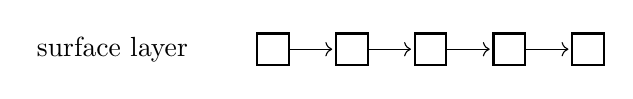
\begin{tikzpicture}[shorten >=1pt,->,draw=black!100,node distance = 1.3cm, auto]]
 	\def \startnode{1.5cm}
 %	\def\secondrow{1.0cm}
 	\tikzstyle{r-node}=[regular polygon sides=4,draw=black!100,thick,inner sep=0pt,minimum size=4mm]
 	\tikzstyle{annot} = [text width=3cm]
 %	\tikzstyle{annot} = [text width=2.0cm, text centered]
 	% labels
 %	\node[annot] (m-label) at (0,\thirdrow) {hidden-unit vector};
 %	\node[annot] (r-label) at (0, \secondrow) {prediction vector};
 %	\node[annot] (d-label) (0, 0) {observed data vector};
 	% hidden layer
 	\node[annot] (surface-label) at (0cm,0cm) {surface layer};
 %	\node[annot] (r-label) at (0, \secondrow) {prediction vector};
 %	\node[annot] (d-label) (0, 0) {observed data vector};
	
 	% surface layer
 	\node[r-node] 	(r0)	at (\startnode,0cm)		{};
 	\node[r-node] 	(r1)	at (2.5cm, 0cm)		{};
 	\node[r-node] 	(r2)	at (3.5cm,0cm)	 	{};
 	\node[r-node] 	(r3)	at (4.5cm,0cm) 		{};
 	\node[r-node] 	(r4) 	at (5.5cm,0cm)   		{};
	
 	\path (r0)	edge	node	{}	(r1)
 		(r1)	edge	node	{}	(r2)
 		(r2)	edge	node	{}	(r3)
 		(r3)	edge	node	{}	(r4);
 \end{tikzpicture}
 \end{center}
 \caption{Sequential linear architecture.}
 %. Each representational unit depends on the preceding unit, and no unit exists outside of the surface layer.}
 \label{fig:seq-lin}
 \end{figure}

% The intuition behind the LSV/LPV method is related to that behind the entropy-based methods in natural language processing:
% %In fact, LSV generally increases/decreases as entropy increases/deceases: 
% At any given point \emph{within} a morpheme, the next letter is fairly predictable, which generally coincides with a smaller number of succeeding letter types. But at the border between two morphemes, the next letter is much less predictable. This low predictability generally translates to a much larger set of options for the succeeding letter (i.e., a higher LSV). However, it out that LSV is not always a reliable indicator of morpheme boundaries. \cite{hammarstrom:2011}, for example, provide LPV counts for the word \textit{disturbance}. 
% The highest count (25) 
% %(i.e., 25 of the 26 possible letters in the English alphabet) 
% occurs between \textit{disturbanc} and \textit{e}, An LPV-based analysis would thus yield an incorrect result in this case, a consequence of the fact that \textit{e} is such a ubiquitous word-final letter in English spelling. 

%Goldsmith
% More recent linear sequential methods
% %have thus abandoned LSV/LPV, often in favor of
% use frequency-based heuristics.  \cite{goldsmith:2001}, for example,
% uses a score based on pointwise mutual information (PMI) to
% approximate the likelihood that a given character $n$-gram
% %$c_{1}c_{2}...c_{n}$ 
% is a morphemic unit.
% % In particular, the PMI of the characters $c_{1},
% % c_{2}, ..., c_{n}$ is multiplied by the relative frequency of the
% % $n$-gram $c_{1}c_{2}...c_{n}$. \cite{goldsmith:2001} obtains candidate
% % suffixes by taking the $n$-grams that are ranked highest according to
% % this score.
% %(i.e., the count of $c_{1}c_{2}...c_{n}$ divided by the total count of all $n$-grams).  
% %
% %Moon
% \cite{moon-et-al:2009} applies \textit{tries} to the task of finding stems and
% affixes, to store recurring character sequences in the search for recurring character sequences.
% % A number of other researchers have done the same.
% % Tries are useful for learning concatenative morphology because they
% % compactly store recurring character sequences.
% %that are repeated a group of words. by sets of words beginning with the same character. 
% % Each node in a trie represents a certain prefix string (with the root node representing the empty string), 
% % and every path proceeding out from a node represents a possible succeeding character. 
% % Thus, even though tries are tree data structures, 
% In all cases, the methods process data in a sequential manner and
% represent morphological relationships linearly, lacking hidden nodes.

% , and every path through a trie is deterministic.
% \cite{moon-et-al:2009} depart from other trie-based methods in using
% document boundaries to approximate semantic context.  This helps them
% weed out spurious analyses like the \textit{disturbanc}+\textit{e}
% example above, but it does not change the fundamentally sequential and
% linear nature of their approach.

\subsection{Non-sequential linear algorithms}
\label{subsec:nonseq-lin}
In the non-sequential linear (NSL) type of algorithm, shown in figure~\ref{fig:nonseq-lin}, the representational units are generally not raw characters, but rather \emph{features}, i.e., binary variables representing the presence or absence of particular properties.
%specifying whether or not a word has a certain property. 
Features in non-sequential algorithms need not correspond to contiguous chunks of the original string; for example, features like the following are perfectly valid: ``\textit{t} precedes \textit{i} within $\delta$ characters" and ``\textit{t} precedes \textit{b} within $\delta$ characters," where the character pairs \emph{t..i} and \emph{t..b} are discontiguous as long as $\delta \ne 0$. Notice that such features cannot really be ordered; each is either \textsc{true} or \textsc{false} irrespective of order.
All non-sequential algorithms---of which NSL algorithms are a subcategory---view a given word's features as being unordered, i.e., as being sequentially unrelated to each other. 
But while NSL algorithms are non-sequential, they are linear because they incorporate no hidden units. Thus, even though an NSL algorithm's features may refer to discontiguous subsequences of characters, they are nonetheless restricted to representing only properties that are overtly present in the surface layer of characters. 

One NSL example is the algorithm of \cite{poon-et-al:2009}, which uses log-linear models to induce morphological segmentations for Arabic and Hebrew. 
Log-linear models are inherently non-sequential because they treat all features as independent, estimating a global joint probability for the entire bag of features. 
%Sequential models, in contrast, estimate conditional probabilities based on sequential dependencies between features
The algorithm of \cite{poon-et-al:2009} in particular searches for the set of parameters $\theta$ that maximizes the joint probability of a corpus $W$ and a morphological segmentation $S$, i.e., $P(W,S| \theta) = P(W|S; \theta) \cdot P(S| \theta)$. The segmentation $S$ is encoded by a set of features.
%They generate candidate segmentations via Gibbs sampling. For each candidate, they extract a feature set

%Log-linear models are well-suited for large numbers of arbitrarily defined features. 
\cite{poon-et-al:2009} use two categories of features to encode a morphological segmentation: \textit{morpheme features} and \textit{morpheme context} features.
The former encode (potential) morpheme types and their frequencies, e.g., \texttt{vlAv:5} and \texttt{w:31}. The 
latter encode context types and their frequencies, where a \emph{context} consists of the $n$ characters preceding and succeeding a (potential) morpheme;
%the character bigrams to the left and right of a potential morpheme, 
e.g., the feature \texttt{\#w\_wn:12} would represent a context whose left side consists of \textit{w} preceded by the word boundary, whose right side is the bigram \textit{wn}, and whose frequency is 12. Importantly, these context features overlap. That is, in \texttt{\#w\_wn:12}, the \textit{w} and \textit{wn} are themselves morphemes whose contexts must be extracted.
This feature overlap is made possible by the non-sequentiality of log-linear models.
%is on the right, , respectively, and whose frequency of this particular context as 12.
%s that the left context is the character \textit{w} preceded by the word boundary, the right context is the character bigram \textit{wn}, and the frequency of this particular context is 12).
% and \textand the characters \textit{w} and \textit{n} are on the right potential morpheme\textit{w} on the left 
%and the characters \textit{w} and \textit{n} on the right).
%Note, however, that 

Note, however, that log-linear models can handle much more non-sequentiality than this. Indeed, since a log-linear models is inherently non-sequential, it accommodate any sort of non-sequential feature. 
%one can incorporate into log-linear model.
%feature %or combination of feature types 
%in a log-linear model.  
One could, for example, incorporate
features representing discontiguous bigrams,
as already noted.
 One could also combine contiguous and discontiguous bigram features in the same feature set.
%for example, have features representing both contiguous and discontinous bigrams in the same feature set.
%However, one in principle could use any sort of feature in a log linear model, such as a feature type representing discontiguous bigrams, for example.
%Each feature represents the both corpus and the segmentation jointly, and a fully specified set of features thus represents an entire segmented corpus;
%but there is no limit on the variety or quantity of features one can incorporate into a log-linear model.
% Why is a log linear model non-sequential?
%Log-linear models are inherently non-sequential because they treat all features as independent, estimating a global joint probability for the entire bag of features. Sequential models, in contrast, estimate conditional probabilities based on sequential dependencies between features.
% Why is a log linear model non-sequential?
And yet it is not the nature of the features themselves that makes an algorithm non-sequential, but rather the lack of sequential relationships between features. The algorithm of \cite{poon-et-al:2009} is non-sequential because it does not process features in a particular order.
% Why is Poon et al's algorithm linear?
It is, however, linear because it incorporates no hidden units to mediate associations between features.

%\cite{poon-et-al:2009} incorporate no latent variables, however. 
%Their representation of morphological structure makes reference only to the the surface layer of graphemes. Their morpheme features are limited to  contiguous grapheme sequences, 
%and their morpheme context features encode only extreme left and right contexts, 
%thus assuming no internal boundaries (i.e., no morpheme interruptions).
%%They generate candidate segmentations via Gibbs sampling, but, for an $n$-length word, they consider 
%Because it only acknowledges the surface layer of text, the algorithm of \cite{poon-et-al:2009} can only isolate stems and affixes, not the discontiguous roots and patterns of Arabic and Hebrew.

%\paragraph{Non-sequential linear algorithms}
%\label{subsec:nonseq-lin}
%
%Like SL algorithms, \textbf{non-sequential linear} (NSL) algorithms consist only of surface units, having no hidden layer, hence their linearity. NSL algorithms are different in that there are no dependencies between representational units. Each unit is independent of other units, hence their \textit{non-sequential} characterization.
%%They consist only of surface units, hence their linearity. What sets NSL algorithms apart is the lack of dependencies between these units, h
%%illustrated in figure~\ref{fig:nonseq-lin}, 
%%there are no dependencies between representational units, but also no
%%hidden units.
%%; i.e., all representational units reside in the surface layer.  
%As one example, \cite{poon-et-al:2009} use log-linear models to induce
%morphological segmentations for Arabic and Hebrew. 
%% Their algorithm
%% searches for the set of parameters $\theta$ that maximizes the joint
%% probability of a corpus $W$ and a segmentation $S$ (i.e., $P(W,S|
%% \theta)$).
%% = P(W|S; \theta) \cdot P(S| \theta)$.
%%They generate candidate segmentations via Gibbs sampling. For each candidate, they extract a feature set
%% Log-linear models are well-suited for large numbers of arbitrarily
%% defined features.
%% \cite{poon-et-al:2009} use morpheme features and morpheme context
%% features.  The former category specifies a morpheme type and its
%% frequency, e.g., \texttt{vlav:1} and \texttt{w:2}.  The latter
%% category indicates the character bigrams to the left and right of a
%% given morpheme, e.g., \texttt{\#w\_wn:1} (a word boundary followed by
%% the character \textit{w} on the left and the characters \textit{w} and
%% \textit{n} on the right).  Note, however, that one could use any type
%% of feature or combination of feature types with a log-linear
%% model. One could, for example, have features representing both
%% contiguous and discontinues bigrams in the same feature set.
%%
%%However, one in principle could use any sort of feature in a log linear model, such as a feature type representing discontiguous bigrams, for example.
%%Each feature represents the both corpus and the segmentation jointly, and a fully specified set of features thus represents an entire segmented corpus;
%%but there is no limit on the variety or quantity of features one can incorporate into a log-linear model.
%% Why is a log linear model non-sequential?
%Log-linear models are non-sequential because they treat all features
%as independent, estimating a global joint probability.
%%for the entire bag of features.
%% Sequential models, in contrast, estimate conditional probabilities
%% based on sequential dependencies between features.
%% Why is Poon et al's algorithm linear?
%% \cite{poon-et-al:2009} incorporate no latent variables,
%% %, however, 
%% %Their representation of morphological structure makes 
%% referencing only the the surface layer of graphemes.
%% Their morpheme
%% features are limited to contiguous grapheme sequences, and their
%% morpheme context features encode only extreme left and right contexts,
%% thus assuming no internal boundaries (i.e., no morpheme
%% interruptions).  
%Even though such a log-linear model allows for any type of feature,
%including both contiguous and discontiguous $n$-grams,
%%They generate candidate segmentations via Gibbs sampling, but, for an $n$-length word, they consider  
%the algorithm ultimately can only isolate stems and affixes, because
%it only acknowledges the surface layer of text.
%%, and not discontiguous roots and patterns.
%% of Arabic and Hebrew.

 \begin{figure}[h]
 %\begin{minipage}{.3\textwidth}
 \begin{center}
 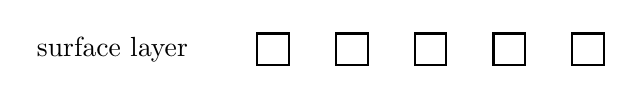
\begin{tikzpicture}[shorten >=1pt,->,draw=black!100]
 	\def \startnode{1.5cm}
 %	\def\secondrow{1.0cm}
 	\tikzstyle{r-node}=[regular polygon sides=4,draw=black!100,thick,inner sep=0pt,minimum size=4mm]
 	\tikzstyle{annot} = [text width=3cm]
 	% labels
 	\node[annot] (surface-label) at (0cm,0cm) {surface layer};
 %	\node[annot] (r-label) at (0, \secondrow) {prediction vector};
 %	\node[annot] (d-label) (0, 0) {observed data vector};
	
 	% surface layer
 	\node[r-node] 	(r0)	at (\startnode,0cm)		{};
 	\node[r-node] 	(r1)	at (2.5cm, 0cm)		{};
 	\node[r-node] 	(r2)	at (3.5cm,0cm)	 	{};
 	\node[r-node] 	(r3)	at (4.5cm,0cm) 		{};
 	\node[r-node] 	(r4) 	at (5.5cm,0cm)   		{};
	
 %	\path (r0)	edge	node	{}	(r1)
 %		(r1)	edge	node	{}	(r2)
 %		(r2)	edge	node	{}	(r3)
 %		(r3)	edge	node	{}	(r4);
 \end{tikzpicture}
 \end{center}
 \caption{Non-sequential linear architecture}
 
 %. No dependencies exist between representational units, and no unit exists outside of the surface layer.}
 \label{fig:nonseq-lin}
 \end{figure}

% \cite{poon-et-al:2009} use morpheme features and morpheme context
% features.  The former category specifies a morpheme type and its
% frequency, e.g., \texttt{vlav:1} and \texttt{w:2}.  The latter
% category indicates the character bigrams to the left and right of a
% given morpheme, e.g., \texttt{\#w\_wn:1} (a word boundary followed by
% the character \textit{w} on the left and the characters \textit{w} and
% \textit{n} on the right).  Note, however, that one could use any type
% of feature or combination of feature types with a log-linear
% model. One could, for example, have features representing both
% contiguous and discontinues bigrams in the same feature set.


\subsection{Sequential nonlinear algorithms}
\label{subsec:seq-nonlin}
% First, what sort of algorithms are sequential nonlinear?
The sequential nonlinear (SNL) type of algorithm is illustrated in figure~\ref{fig:seq-nonlin}. 
Note in particular the addition of a hidden layer, whose units (the circular nodes)
represent the underlying sources of the surface data's implicit structure.
%account for the surface %the surface units and thus take responsibility for the regularities ac
%for 
%algorithms differ from sequential linear ones in that 
%they add a layer of hidden units for 
%encoding 
%take responsibility for generating the structure implicit
%the regularities %, i.e., the implicit structure, 
%in the surface layer and thus the
%data.
%These hidden units can be viewed as causing or generating the surface data.
SNL algorithms are nonlinear because they incorporate a hidden layer.
However, they are sequential because the hidden layer in an SNL algorithm is sequential; i.e., its component hidden units
%hidden units
are sequentially ordered.
Since the surface units depend on the hidden units, the hidden layer imposes its sequential order on the surface layer. 
%they have a certain each hidden unit depends on its predecessor hidden unit(s). 
% I need to say what the nonlinear aspect brings to the table. If being nonlinear is beneficial, sequential nonlinear algorithms should be better than sequential linear ones. So what do sequential nonlinear algorithms have that sequential linear algorithms don't? How does being nonlinear help them?
% First, what sort of algorithms are sequential nonlinear?

%Sequential nonlinear (SNL) algorithms
%%, illustrated in figure~\ref{fig:seq-nonlin}, 
%differ from sequential
%linear ones by adding a layer of hidden units for encoding the
%structure of the surface layer.
%This makes them nonlinear. 
% They are still sequential, however, in that there are sequential
% dependencies within the hidden layer.
%; i.e., each hidden unit depends on its predecessor hidden unit(s).
%The prototypical example of a sequential nonlinear model is the Hidden
%Markov Model (HMM).  \cite{creutz-and-lagus:2005,
%  creutz-and-lagus:2007} employ an HMM to induce a morphological
%lexicon.
The prototypical SNL model is the Hidden Markov Model (HMM). 
\cite{creutz-and-lagus:2005, creutz-and-lagus:2007} employ an HMM to induce a morphological lexicon, i.e., a list of morpheme-like segments they call \textit{morphs}. 
%, i.e., a list of morpheme-like segments.
%that they call \textit{morphs}.
%sorted in order of increasing morph length. 
%They take a maximum a posteriori (MAP) approach.
Their algorithm seeks to find the lexicon such that $P(lexicon|corpus)$ is maximized. Due to Bayes' theorem, this equates to finding the lexicon that maximizes $P(corpus|lexicon) \cdot P(lexicon)$. The probability $P(corpus|lexicon)$ is computed by an HMM. Each unit in this HMM's hidden layer can take on five possible values: \textit{prefix}, \textit{stem}, \textit{suffix}, \textit{word boundary}, and \textit{non-morpheme}. 
Note how the first four relate sequentially to each other: prefixes must precede stems, stems must precede suffixes, and so on.
%The observation sequence is a segmentation hypothesis, i.e., a candidate segmentation of the corpus into morphs. 
%Candidate segmentations are generated independently of the HMM, as are the transition and emission probabilities. 
%The HMM's role to find likely hidden state sequence, which is computed by the Viterbi algorithm, along with the probability $P(corpus|lexicon)$. 
The hidden layer in this case serves to facilitate the search for the optimal lexicon 
(i.e., segmentation) by providing a means of abstracting away from the literal surface characters.

%The HMM's role is to evaluate each candidate morph sequence. 
% took out the "h"
 \begin{figure}[h]
 %\begin{minipage}{.3\textwidth}
 \begin{center}
 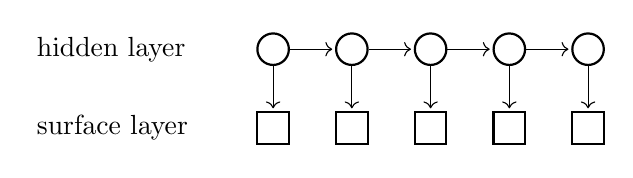
\begin{tikzpicture}[shorten >=1pt,->,draw=black!100]
 	\def \rowtwoht{1.0cm}
 	\def \rowoneht{0.0cm}
 	\tikzstyle{m-node}=[circle,draw=black!100,thick,inner sep=0pt,minimum size=4mm]
 	\tikzstyle{r-node}=[regular polygon sides=4,draw=black!100,thick,inner sep=0pt,minimum size=4mm]
 	\tikzstyle{annot} = [text width=3cm]
 	% labels
 	\node[annot] (hidden-label) at (0cm,\rowtwoht) {hidden layer};
 	\node[annot] (surface-label) at (0cm,\rowoneht) {surface layer};

 %	\node[annot] (d-label) (0, 0) {observed data vector};
	
 	% hidden layer
 	\node[m-node] 	(m0)	at (1.5cm,\rowtwoht)		{};
 	\node[m-node] 	(m1)	at (2.5cm,\rowtwoht)		{};
 	\node[m-node] 	(m2)	at (3.5cm,\rowtwoht)	 	{};
 	\node[m-node] 	(m3)	at (4.5cm,\rowtwoht) 		{};
 	\node[m-node] 	(m4) 	at (5.5cm,\rowtwoht)   		{};
	
 	% surface layer
 	\node[r-node] 	(r0)	at (1.5cm,\rowoneht)		{};
 	\node[r-node] 	(r1)	at (2.5cm,\rowoneht)		{};
 	\node[r-node] 	(r2)	at (3.5cm,\rowoneht)	 	{};
 	\node[r-node] 	(r3)	at (4.5cm,\rowoneht) 		{};
 	\node[r-node] 	(r4) 	at (5.5cm,\rowoneht)   		{};
	
 	\path (m0)	edge	node	{}	(m1)
 		(m1)	edge	node	{}	(m2)
 		(m2)	edge	node	{}	(m3)
 		(m3)	edge	node	{}	(m4);
		
 	\path (m0)	edge	node	{}	(r0)
 		(m1)	edge	node	{}	(r1)
 		(m2)	edge	node	{}	(r2)
 		(m3)	edge	node	{}	(r3)
 		(m4)	edge	node	{}	(r4);
			
 \end{tikzpicture}
 \end{center}
 \caption{Sequential nonlinear architecture}
 % . Sequential dependencies only exist between hidden units, 
 % not between the observed units of the surface layer. The hidden units ``cause" the surface units.}
 \label{fig:seq-nonlin}
 \end{figure}

\subsection{Non-sequential nonlinear algorithms}
\label{subsec:nonseq-nonlin}
% Intro
 Like sequential nonlinear (SNL) algorithms, \textit{non}-sequential
 nonlinear (NSNL) algorithms incorporate a hidden layer whose units generate the observed
 units of the surface layer.
The difference is that the hidden layer in an NSNL algorithm is \emph{non-sequential}; 
i.e., the algorithm computes the values of all hidden units in parallel rather than in a sequence.
The surface layer in a NSNL algorithm is also non-sequential.
 %dependencies.
 Thus, every unit---whether hidden or surface---is entirely independent
 within its own layer. Figure~\ref{fig:nonseq-nonlin} illustrates the NSNL framework; notice that no two nodes with the same layer are connected by an arc.
This intra-layer independence allows a hidden unit to associate with
any combination of surface units, whether contiguous or discontiguous
%(see Figure \ref{fig:nonseq-nonlin}).

 \begin{figure}[tb]
 %\begin{minipage}{.3\textwidth}
 \begin{center}
 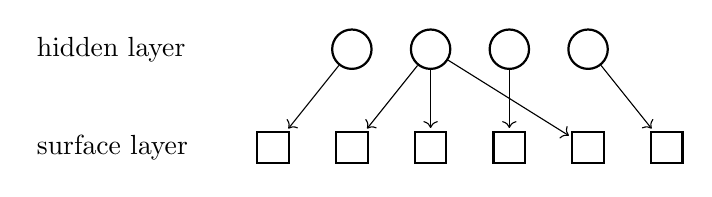
\begin{tikzpicture}[shorten >=1pt,->,draw=black!100] %,scale=.95]
 	\def \rowtwoht{1.25cm}
 	\def \rowoneht{0.0cm}
 	\tikzstyle{m-node}=[circle,draw=black!100,thick,inner sep=0pt,minimum size=5mm]
 	\tikzstyle{r-node}=[regular polygon sides=4,draw=black!100,thick,inner sep=0pt,minimum size=4mm]
 	\tikzstyle{annot} = [text width=3cm]
 	% labels
 	\node[annot] (hidden-label) at (0cm,\rowtwoht) {hidden layer};
 	\node[annot] (surface-label) at (0cm,\rowoneht) {surface layer};

 %	\node[annot] (d-label) (0, 0) {observed data vector};
	
 	% hidden layer
 	\node[m-node] 	(m0)	at (2.5cm,\rowtwoht)		{};
 	\node[m-node] 	(m1)	at (3.5cm,\rowtwoht)		{};
 	\node[m-node] 	(m2)	at (4.5cm,\rowtwoht)	 	{};
 	\node[m-node] 	(m3)	at (5.5cm,\rowtwoht) 		{};
	
 	% surface layer
 	\node[r-node] 	(r0)	at (1.5cm,\rowoneht)		{};
 	\node[r-node] 	(r1)	at (2.5cm,\rowoneht)		{};
 	\node[r-node] 	(r2)	at (3.5cm,\rowoneht)	 	{};
 	\node[r-node] 	(r3)	at (4.5cm,\rowoneht) 		{};
 	\node[r-node] 	(r4) 	at (5.5cm,\rowoneht)   		{};
 	\node[r-node] 	(r5) 	at (6.5cm,\rowoneht)   		{};
	
 	\path (m0)	edge	node	{}	(r0)
 		(m1)	edge	node	{}	(r1)
 		(m2)	edge	node	{}	(r3)
 		(m1)	edge	node	{}	(r2)
 		(m1)	edge	node	{}	(r4)
 		(m3)	edge	node	{}	(r5);
		
 \end{tikzpicture}
 \end{center}
 \caption{Non-sequential nonlinear architecture}
 %. Neither layer contains sequential dependencies; every unit is independent within its own layer. Each hidden unit is thus free to cause any combination of observed units.}
 \label{fig:nonseq-nonlin}
 \end{figure}

%The NSNL type can take many forms.  \cite{baroni-et-al:2002}, for
%example, implicitly detect hidden units by computing edit distance for
%pairs of words.
%% The
%% Levenshtein algorithm finds the minimum number of edit operations
%% (typically allowing substitutions, deletions, and insertions) required
%% to change a \textit{source} word into a \textit{target} word.  In
%% addition to edit distance and edit operations, the algorithm can align
%% the characters of the source with those of the target word.  
%From an alignment, one can extract the two words' (potentially
%discontiguous) common subsequence.  Thus, one may view the alignment
%as showing
%%indicative of
%a single hidden unit behind the surface occurrences of the
%subsequence.  For example, for the Hebrew words \textit{dibr} `he
%spoke' and \textit{mdbr} `he is speaking', the discontiguous root
%\textit{d.b.r} is found.
% Of course, a common subsequence does not necessarily indicate a
% morphological relationship; consider, for instance, the English pair
% To avoid finding spurious relationships
% (cf. \textit{pork}/\textit{park}), \cite{baroni-et-al:2002} compute a
% semantic similarity score, based on mutual information, to combine
% with this orthographic similarity.
% based on minimum edit distance.
%orthographic similarity score.

The NSNL type can take many forms. 
\cite{baroni-et-al:2002}, for example, detect implicit causal units by computing 
the Levenshtein alignments for pairs of words. 
The Levenshtein algorithm finds the minimum number of edit operations 
(typically allowing substitutions, deletions, and insertions) required to change 
a \textit{source} word into a \textit{target} word.
An alignment of the source and target characters is obtained as a by-product 
of computing the edit operations. 
%In addition to edit distance and edit operations, the algorithm can align the 
characters of the source with those of the target word. 
From the alignment, one can extract the (not necessarily contiguous) 
subsequence held in common by the two words.
%One might view the common subsequence as suggesting a sin
Thus, one may view the alignment as suggesting a single causal unit behind 
both occurrences of the subsequence, i.e., as a kind of implicit hidden unit, 
as it were.
For example, the alignment in figure~\ref{fig:lev-align} implies a single cause 
behind both occurrences of the subsequence \textit{dbr}.
Of course, a common subsequence does not necessarily indicate a 
morphological relationship; 
consider, for instance, the English pair \textit{pork}/\textit{park}. 
To avoid finding spurious relationships, 
\cite{baroni-et-al:2002} compute a semantic similarity score based on 
mutual information, 
combining it with an orthographic similarity score based on minimum 
edit distance.

 \begin{figure}[htb!]
 %\begin{minipage}{.3\textwidth}
 \begin{center}
 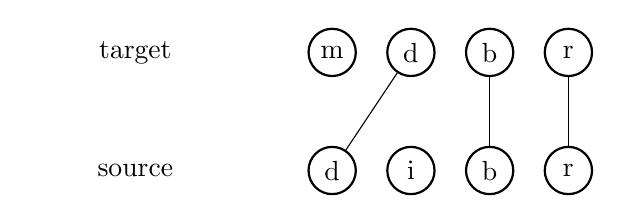
\begin{tikzpicture}[draw=black!100]
 	%[shorten >=1pt,->,draw=black!100]
 	\def \rowtwoht{1.5cm}
 	\def \rowoneht{0.0cm}
 	\tikzstyle{m-node}=[circle,draw=black!100,thick,inner sep=0pt,minimum size=6mm]
 	\tikzstyle{r-node}=[circle,draw=black!100,thick,inner sep=0pt,minimum size=6mm]
 	\tikzstyle{annot} = [text width=2.5cm, text centered]
 	% labels
 	\node[annot] (hidden-label) at (0cm,\rowtwoht) {target};
 	\node[annot] (surface-label) at (0cm,\rowoneht) {source};

 %	\node[annot] (d-label) (0, 0) {observed data vector};
	
 	% hidden layer
 	\node[m-node] 	(m0)	at (2.5cm,\rowtwoht)		{m};
 	\node[m-node] 	(m1)	at (3.5cm,\rowtwoht)		{d};
 	\node[m-node] 	(m2)	at (4.5cm,\rowtwoht)	 	{b};
 	\node[m-node] 	(m3)	at (5.5cm,\rowtwoht) 		{r};
	
 	% surface layer
 	\node[r-node] 	(r0)	at (2.5cm,\rowoneht)		{d};
 	\node[r-node] 	(r1)	at (3.5cm,\rowoneht)		{i};
 	\node[r-node] 	(r2)	at (4.5cm,\rowoneht)	 	{b};
 	\node[r-node] 	(r3)	at (5.5cm,\rowoneht) 		{r};
 	%\node[r-node] 	(r4) 	at (6.5cm,\rowoneht)   		{};
 	%\node[r-node] 	(r5) 	at (7.5cm,\rowoneht)   		{};
	
 	\path (m1)	edge	node	{}	(r0)
 		(m2)	edge	node	{}	(r2)
 		(m3)	edge	node	{}	(r3);
 %		(m3)	edge	node	{}	(r3)
 %		(m1)	edge	node	{}	(r4)
 %		(m3)	edge	node	{}	(r5);
		
 \end{tikzpicture}
 \end{center}
 \caption{The minimum-edit-distance alignment for the Hebrew words \textit{dibr} `he spoke' and \textit{mdbr} `he is speaking'. The discontiguous root \textit{d.b.r } is discovered by aligning \textit{dibr} with \textit{mdbr} and extracting the common subsequence.}
 \label{fig:lev-align}
 \end{figure}


Other authors simulate a nonlinear, multi-tier representation by 
separating the 
learning process into two or more phases.
The first phase classifies individual literal characters into abstract categories 
that are then 
used by a second phase (and perhaps subsequent phases) to perform other 
aspects of the analysis.
Multiple phases occurring at different times can thus replicate the effects 
of multiple simultaneous levels of representation.
This is the approach taken by \cite{rodrigues-and-cavar:2005} to induce 
the non-concatenative morphology of Arabic. 
%Following the statistical constraint-based method of \cite{elghamry:2005}, 
Their first phase identifies root radicals according to the statistical 
constraint-based method of \cite{elghamry:2005}. 
For each word in their corpus, 
they generate a set of candidate triliteral roots according to 
constraints derived from the tendencies of Arabic roots as observed in corpora. 
In particular, any 3-length subsequence is admitted into the candidate set 
if and only if it satisfies both of the following:
%, which in Arabic comprise both a consonantal root and a vocalic pattern. A string is allowed into a word's candidate stem set if and only if it satisfies the following constraints, which are based on the tendencies of Arabic roots as observed in corpora.
\begin{enumerate} 
\item No two consecutive radicals may be separated by more than two characters.
\item No more than four characters intervene between the first and third radicals.
\end{enumerate}
%\item ``The distance between the first and third radicals cannot be greater than five" \citep[][p. 3]{elghamry:2005}. 
Then, a statistical score is computed for each candidate, and the one with the highest score is selected as the root.
Once the roots---and thus the stems---have been isolated by the first phase, the second phase identifies the concatenative affixes through a separate methodology.

% Goldsmith and Xanthos
An alternative first-phase strategy can be found in \cite{goldsmith-and-xanthos:2009}, 
who present methods for
partitioning a phonemic inventory into a class of consonants and a class of vowels. 
Their paper does not go into automatic morphological analysis, but it is not difficult to see how C and V classes could be useful to a multi-phase morphological analyzer.
The first phase would partition the phonemic inventory and, for each word, label each phoneme/grapheme as either a consonant or vowel, thus creating a sort of CV skeleton similar to the segmental tier of autosegmental phonology.
Subsequent phases would then use these CV skeletons to isolate roots, patterns, and other morphemes.
%The second phase (and perhaps subsequent phases) would then use template to Such a template would be helpful to subsequent phases as they go about isolating the root, pattern, and other morphemes. 
%To delimit distinct morphemes, the linear approach must 

While the NSNL approaches described in this section provide a means for detecting discontiguous morphemes, they are not without their weaknesses. 
% Baroni
%% Mucho filtering
The algorithm of \cite{baroni-et-al:2002} must filter out a large proportion of its input corpus, accepting only the words with relative frequencies of less than 0.01 percent; which are presumed to be content words.
%% Arbitrary thresholds
It also relies on arbitrary thresholds; e.g., the threshold for orthographic similarity measure (i.e., $1 - $ the normalized minimum edit distance) is set at 0.5, although there is no obvious reason why this should be so.
Note also that behind this threshold is the assumption that morphologically related words share at least half of their characters, which is not necessarily true. Such an assumption would be especially problematic for highly agglutinative languages, 
in which it is not uncommon for a stem to comprise a minority of a word's characters.
Moreover, the Levenshtein edit-distance approach is only capable of comparing words pairwise, which only allows morphological relationships to be expressed on a pairwise basis. This is a consequence of the lack of an explicitly encoded hidden causal layer; an explicit (as opposed to implicit) hidden layer could easily mediate multi-way associations among surface layer components.                                   

% Rodrigues and Cavar
%% Only tri-literal roots
Moreover, \cite{rodrigues-and-cavar:2005}, following \cite{elghamry:2005}, limit their algorithm's search to triliteral roots in order to reduce the problem's complexity, even though quadriliteral roots are not uncommon in Hebrew or Arabic.
%% Reasonable constraints, but constraints nonetheless. A truly general algorithm wouldn't need constraints. 
And while their two constraints on candidate-root generation are quite reasonable, these constraints are particular to the case of Semitic morphology, and thus they would not be required by a truly general algorithm.

Finally, none of the works discussed in this section represents both the hidden layer and surface layer simultaneously in a single, straightforward model. In contrast, the Multiple Cause Mixture Model (MCMM) \citep{saund:94} is an NSNL algorithm that explicitly represents both surface and hidden nodes in a single graphical model. The MCMM is the focus of the next section.


\chapter{Graph-Theoretic Foundation}
\label{ch:graph}
\section{Introduction}
The purpose of this chapter is to
%connect the logical dots between 
establish a link from autosegmental morphology to bipartite graphs. We will then easily be
able to link bipartite graphs to the multiple cause mixture model (MCMM), since, as we will see,
MCMMs are bipartite graphs.
%is to motivate the use of an \ac{MCMM} as Multimorph's 
%learning framework. 
The key concept in this chapter will be the \emph{bipartite} graph, 
a type of graph so named because its nodes can be partitioned into two subsets according 
to criteria which we discuss below. 
We will see that bipartite graphs have properties that are essential 
to the tasks of modeling and learning nonconcatenative morphology.
% a type of graph with two sets of nodes such that only nodes of different sets are connected. Within each set, there are no connections. This intra-layer independence engenders some important properties, as we shall see.
In section~\ref{sec:bipartite}, we will describe the mathematical concept of the 
\emph{bipartite graph}, placing particular importance on the properties that make this type 
of graph naturally conducive to modeling nonconcatenative morphology. %We shall demonstrate that bipartite graphs are essential for the modeling of nonconcatenative morphology (and thus morphology in general). 

In section~\ref{sec:autoseg-bipart}, we will take a fresh look at McCarthy's 
autosegmental framework for morphology \citep{mccarthy:1981} in light of the 
properties of the bipartite graph. We will thus see that 
McCarthy's 
autosegmental framework can be reduced to a bipartite graph.
% but also that the properties of 
%bipartite graphs are essential for the modeling of nonconcatenative morphology.
% naturally well-suited to modeling non-concatenative morphology. and more than that, we will argue that bipartite graphs are general that ultimately derive from these properties two necessary conditions that morphological models must satisfy in order to be capable of modeling bipartite graphs two criteria that a morphological model must satisfy We will see that McCarthy's framework is itself a bipartite graph. and re
Finally, in section~\ref{sec:mcmm-bipartite}, we will see that the \ac{MCMM} is also a bipartite graph.
Bipartiteness will ultimately serve as a common denominator, so to speak, between the autosegmental formalism and the MCMM, providing a means of expressing the autosegmental formalism as an MCMM.
%via its biparteness, its compatibility with %is a bipartite graph, 
%and that, consequently, it is compatible, so to  speak, with autosegmental morphology. 
%In other words, an MCMM can serve as a
%a computational ``wrapper," so to speak, for McCarthy's autosegmental theory, a 
%means whereby it can be specially packaged for use in a machine learning system. 
 
%itself has a bipartite architecture, which is to say that it can be represented as and thought of as a bipartite graph without information loss.  essentially bipartite in its architecture, and that it ; we will see that the autosegmental framework is essentially a bipartite graph. We shall then observe in section~\ref{sec:bipartite} that an \ac{MCMM} is itself a bipartite graph, and that autosegmental morphology and \ac{MCMM}s have the same graphical properties. From this point, the conclusion follows that an From a theoretical perspective, therefore, it is a sound choice to use the \ac{MCMM} as a computational``wrapper," as it were, for McCarthy's theoretical autosegmental framework, to package for it for use a machine learning system. 
%The argumentation in this chapter will proceed as follows: 
%\begin{enumerate}
%\item We shall first demonstrate that the autosegmental morphological framework of \cite{mccarthy:1981} is, in its essence, a bipartite graph.
%\item We shall then observe that an \ac{MCMM} is quite clearly a bipartite graph. 
%\item From these two points, it follows that autosegmental morphology and \cm
%\end{enumerate}

%We shall first show that McCarthy's autosegmental morphological framework of \cite{mccarthy:1981} is a bipartite graph. We we shall show that an MCMM is a bipartite graph. And connecting the latter point to the former, %the latter point to the former, 
%we shall conclude that because the MCMM and McCarthy's autosegmental formalism 
%are both bipartite graphs, the MCMM is a very appropriate learning framework for 
%modeling autosegmental morphology and thus for learning nonconcatenative 
%morphology. The \ac{MCMM}, therefore, is well-suited to serve as a computational implementation of autosegmental morphology. %mathematically, and in particular, graph-theoretically. , we shall introduce the \emph{multipartite graphs}, 
%particularly \emph{bipartite graphs}, as well as discuss their relationship to autosegmental morphology, and hence their significance to the problem of
%learning non-concatenative morphology.   
%relevance to the problem of leand their relationship 
%to autosegmental morphology.
% which are a subset, i.e., special case, of multipartite graphs. 
\section{Bipartite Graphs}\label{sec:bipartite}
A \emph{multipartite} is a graph whose 
whose nodes are partitioned into $N$ disjoint subsets of 
\emph{mutually nonadjacent} nodes, i.e., $N$ sets such that no two
nodes within the \emph{same} set are connected by an edge. A bipartite graph
is simply multipartite graph such that $N = 2$. Thus, a bipartite graph is defined 
as follows:
%graph that satisfies the following: i.e., it has two partitions of nodes  That is, a graph is \textbf{bipartite} if it satisfies the following
%criteria in \ref{ex:bipartite}.
%\begin{definition} A graph is \textbf{bipartite} if it satisfies the following criteria:
%\begin{enumerate}
%\item The graph's nodes are separated into two disjoint sets (or partitions).
%\item Within each partition, all nodes are independent, i.e., mutually nonadjacent.
%\end{enumerate}
%\theoremstyle{definition}
%\begin{definition}{Bipartite Graph}
%A bipartite graph is a set of nodes divided into two sets such that
%no two nodes of the same set are connected.
%\begin{description}
%\item[Part 1:] Its nodes are partitioned into two sets
%\item[Part 2:] Two nodes are members of the same set if and only if they are \emph{not} connected by an edge.
%\end{description}
%A graph such that
%\begin{criterion}
%Its nodes are divided into two partitions. 
%\end{criterion}
%\end{definition}

\begin{exe} 
	\ex \label{ex:bipartite} A \textbf{bipartite} graph is  
	\begin{xlist} 
		\ex \label{ex:bipartite1}%{\textsc{Nonlinearity}}.  %A model is \emph{nonlinear} 
	 	A graph whose nodes are partitioned into two disjoint subsets \\ such that: %, or partitions. \label{ex:bipartite1} %separated into two disjoint sets, or partitions. %eparately for m  as being separate from (or outside of) the the phonological (or segmental) tier.  % is a property wherein morphs are represented as being separate from the segmental tier.
		\ex \label{ex:bipartite2}%Within each partition, nodes are mutually non-adjacent. % ; 
		Two nodes are members of the same subset if and only if 
		they are \emph{not} connected.
	\end{xlist}
\end{exe}
The two parts of this definition---parts~m(\ref{ex:bipartite1}) and (\ref{ex:bipartite2})---are equivalent to the properties of nonlinearity and 
nonsequentiality, respectively, first presented as defintions~\ref{def:nl} and \ref{def:ns} in chapter~\ref{ch:intro}. We restate it here for the sake of convenience and to make the correspondences clear:
%For convenience, we restate their definitions here:
% as (\ref{ex:criteria1-again}) and (\ref{ex:criteria2-again}):
%\begin{exe} \label{ex:criteria1-again} \ex \begin{xlist}
	\begin{description}
	\item[Nonlinearity:]
	%\ex {\textsc{Nonlinearity}}.  %A model is \emph{nonlinear} 
	A model is \textbf{nonlinear} if each of its morphs occupies a tier that is \emph{not} the phonological tier.
%	Morphs must be represented separately 
%	from the surface (or phonological) tier, i.e., as residing on tiers distinct from 
%	the phonological tier. %\label{ex:criteria1-again}
	%eparately for m  as being separate from (or outside of) the the phonological (or segmental) tier.  % is a property wherein morphs are represented as being separate from the segmental tier.
	\item[Nonsequentiality:]
	%\ex {\textsc{Nonsequentiality}}.
	%Each morph tier is required to be orthogonal to all other morph tiers. %\label{ex:criteria2-again}
	A model is \textbf{nonsequential} if \textbf{no two morphs} occupy the \emph{same} tier. This is to say that all morphs are independent, i.e., that there are no morph-to-morph connections.
	%\end{xlist}
%\end{exe}
	\end{description}
Part~(\ref{ex:bipartite1}) of the definition of \emph{bipartite} corresponds to nonlinearity, since both require a partition between two sets of units. The definition of nonlinearity, in particular, requires a partition between morphs and the units of the phonological tier. 
Part~(\ref{ex:bipartite2}) corresponds to nonsequentiality, as both require independence among units of the same set (or tier).

Figure~\ref{fig:gt-bipartite} shows a bipartite graph. The two disjoint subsets are presented as two rows, or layers, of nodes and labeled $M$ and $R$. Within in each layer, all nodes are independent; that is, no node in $M$ is connected to another node in $M$, and the same is true of the nodes in $R$. The only connections are between nodes of different sets. 
As we will see in the next section, the components of the autosegmental formalism map nicely onto this bipartite architecture. %onto these components of
%a bipartite graph.
 
 \begin{figure}[t]
\centering
 \begin{mdframed}
 \centering
 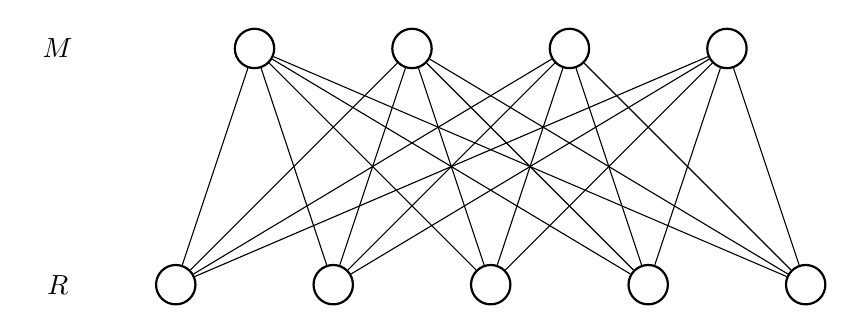
\begin{tikzpicture}[draw=black!100,scale=1.0]
 	\def \rowtwoht{3cm}
 	\def \rowoneht{0.0cm}
 	\tikzstyle{m-node}=[circle,draw=black!100,thick,inner sep=0pt,minimum size=5mm]
 	\tikzstyle{r-node}=[circle,draw=black!100,thick,inner sep=0pt,minimum size=5mm]
 	\tikzstyle{annot} = [text width=1.5em, text centered]
 	\node[annot] (hidden-label) at (-0.5cm,\rowtwoht) {$M$};
 	\node[annot] (surface-label) at (-0.5cm,\rowoneht) {$R$};
 	\node[m-node] 	(m0)	at (2cm,\rowtwoht)		{};
 	\node[m-node] 	(m1)	at (4cm,\rowtwoht)		{};
 	\node[m-node] 	(m2)	at (6cm,\rowtwoht)	 	{};
 	\node[m-node] 	(m3)	at (8cm,\rowtwoht) 		{};
 	% surface layer
 	\node[r-node] 	(r0)	at (1cm,\rowoneht)		{};
 	\node[r-node] 	(r1)	at (3cm,\rowoneht)		{};
 	\node[r-node] 	(r2)	at (5cm,\rowoneht)	 	{};
 	\node[r-node] 	(r3)	at (7cm,\rowoneht) 		{};
 	\node[r-node] 	(r4) 	at (9cm,\rowoneht)   		{};
 	%\node[r-node] 	(r5) 	at (6.5cm,\rowoneht)   		{};
 	\path (r0)	edge	node	{}	(m0)
		(r0)	edge	node	{}	(m1)
		(r0)	edge	node	{}	(m2)
		(r0)	edge	node	{}	(m3)

		(r1)	edge	node	{}	(m0)
		(r1)	edge	node	{}	(m1)
		(r1)	edge	node	{}	(m2)
		(r1)	edge	node	{}	(m3)

		(r2)	edge	node	{}	(m0)
		(r2)	edge	node	{}	(m1)
		(r2)	edge	node	{}	(m2)
		(r2)	edge	node	{}	(m3)
						
		(r3)	edge	node	{}	(m0)
		(r3)	edge	node	{}	(m1)
		(r3)	edge	node	{}	(m2)
		(r3)	edge	node	{}	(m3)

		(r4)	edge	node	{}	(m0)
		(r4)	edge	node	{}	(m1)
		(r4)	edge	node	{}	(m2)
		(r4)	edge	node	{}	(m3);
 		%(m3)	edge	node	{}	(r5);		
 \end{tikzpicture}
 \caption{Bipartite graph}
 %. Neither layer contains sequential dependencies; every unit is independent within its own layer. Each hidden unit is thus free to cause any combination of observed units.}
 \label{fig:gt-bipartite}
  \end{mdframed}
 \end{figure}
%\end{definition}
%\end{definition}
%(i.e., non-adjacent). Conversely, 
%	if two nodes \emph{are} connected (or adjacent), they necessarily belong to different sets. 
%	\emph{This means that \textbf{within} each or partition, all nodes are independent 
%	(i.e., not connected).}


\section{Bipartiteness of the Autosegmental Formalism}\label{sec:autoseg-bipart}
The central aspect of autosegmental theory 
is its \emph{multilinear} architecture, i.e., its use of a 
\emph{segmental tier} along with many \emph{autosegmental tiers} to 
account for the surface forms of words \citet{mccarthy:1981}. The segmental tier is home to the sequence of consonants and vowels that define the linear arrangement of phonological features. Each autosegmental tier is home to a morph. Each morph, therefore, occupies its own distinct plane and is thus external to the segmental tier. The separation of morphs from the segmental tier allows a given morph to connect to nonadjacent phonological segments, as illustrated in figure~\ref{subfig:multilinear-gt}. 
The multilinear architecture of autosegmental theory thus provides a means of
dealing with nonconcatenative morphology. 

One can see this plainly by comparing figures~\ref{subfig:multilinear-gt} and 
\ref{subfig:linear-gt}. Each shows an attempt to analyze the word \emph{hizkir} `he reminded', 
in which the root \textit{z.k.r} (morph $\mu_3$) is interrupted by the /i/ of morph 
$\mu_2$ and is thus a discontinuous, or non-concatenative morph. 
Figure~\ref{subfig:multilinear-gt} is a multilinear autosegmental approach 
(or nonlinear nonsequential type of model described in chapter~\ref{ch:lit-review}), 
whereas figure~\ref{subfig:linear-gt} is a linear approach. The multilinear approach 
is able to recognize the root \textit{z.k.r} as a coherent morph despite its discontinuity. 
The linear approach, by contrast, has no way to group the \textit{r} with the \textit{z} and {k}.

%In figure~\ref{subfig:multilinear-gt}, we see at work the properties \emph{nonlinearity} and \emph{nonsequentiality}, first defined in chapter~\ref{ch:lit-review}.
%Let us restate these properties here as (\ref{ex:criteria1-again}) and (\ref{ex:criteria2-again}).
%\begin{exe} \label{ex:criteria1-again} \ex \begin{xlist}
%	\ex {\textsc{Nonlinearity}}. 	Morphs must be separate from the phonological tier. 
%	\ex {\textsc{Nonsequentiality}}.
%	Each morph tier must be orthogonal to all other morph tiers. \label{ex:criteria2-again}
%	\end{xlist}
%\end{exe}

There is a clear correspondence between these two properties  %(\ref{ex:criteria1-again}) (\ref{ex:criteria2-again})  
and the two components of the definition of \emph{bipartite} in (\ref{ex:bipartite}) above.
The reason for this correspondence is that the autosegmental 
framework is essentially a bipartite graph. 
We can make this clearer simply be rearranging the morph 
nodes $\mu_1$, $\mu_2$, and $\mu_3$. That is, can 
simply move up $\mu_2$ so that it is situated between 
$\mu_1$ and $\mu_3$, i.e., so that all three morphs are 
lined up in a row, as in figure-\ref{fig:autoseg-to-bipartite}. We can then view this row (or vector) of 
morphs as one of the partitions in a bipartite graph.
\begin{figure}[t]
\begin{mdframed}
%\vspace{-20pt}
	\centering
	\subfigure[Multilinear approach\label{subfig:multilinear-gt}]{
	\begin{tikzpicture}[shorten >=1pt,draw=black!100]
	\def \rowtwoht{4cm}
	%\def \weightstwo{3.75cm}
	\def \rowoneht{2cm}
	%\def \weightsone{1.25cm}
	\def \basement{0cm}
	\tikzstyle{m-node}=[text height=6pt,text centered,inner sep=6pt,minimum size=12pt]
	\tikzstyle{r-node}=[text height=6pt,text centered,inner sep=6pt,minimum size=12pt]
	\tikzstyle{d-node}=[text height=6pt,text centered,inner sep=6pt,minimum size=12pt]
	\tikzstyle{annot}=[text width=20ex]
	% labels
	\node[annot] (mtierstop) at (0cm,\rowtwoht) {};
	\node[annot] (segtier) at (0cm,\rowoneht) {surface layer};
	\node[annot] (mtiersbot) at (0cm,\basement) {};
	
	% hidden layer
	\node[m-node] 	(m0)	at (1.7cm,\rowoneht)		{h};
	\node[m-node] 	(m1)	at (2.0cm,\rowoneht)		{i};
	\node[m-node] 	(m2)	at (2.3cm,\rowoneht)		{\textbf{z}};
	\node[m-node] 	(m3)	at (2.6cm,\rowoneht)	 	{\textbf{k}};
	\node[m-node] 	(m4)	at (2.9cm,\rowoneht)	 	{i};
	\node[m-node] 	(m5)	at (3.2cm,\rowoneht)	 	{\textbf{r}};
	
	% reconstructed vector
	\node[r-node] 	(r0)	at (2.3cm,\rowtwoht)		{$\mu_{1}$};
	%\node[r-node] 	(r6) 	at (9.75cm,\rowoneht)   	{$r_J$};
	
	% data vector
	\node[d-node] 	(d0)	at (1.8cm,\basement)		{$\mu_{2}$};
	\node[d-node] 	(d1)	at (2.9cm,\basement)		{$\mu_{3}$};
	%\node[d-node] 	(d6) 	at (9.75cm,\basement)   	{$d_J$};
	
	\path
		(r0)	edge	node	{}	(m2)
		(r0)	edge	node	{}	(m3)
		(r0)	edge	node	{}	(m5)
		%
		(d0)	edge	node	{}	(m0)
		(d0)	edge	node	{}	(m1)
		(d1)	edge	node	{}	(m4);
	\end{tikzpicture}
	%\label{subfig:multilinear-gt}
	} \hspace{2cm}
	\subfigure[Linear approach\label{subfig:linear-gt}]{
	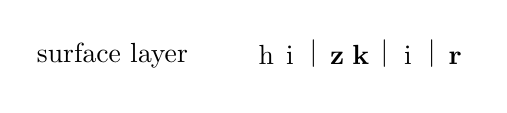
\begin{tikzpicture}[shorten >=1pt,draw=black!100]

	\def \floor{2cm}
	\tikzstyle{f-node}=[text height=6pt,text centered,inner sep=6pt,minimum size=15pt]
	\tikzstyle{annot}=[text width=20ex]
	% labels
	\node[annot] (floorlabel) at (0cm,\floor) {surface layer};
	
	% surface layer
	\node[f-node] 	(f0)	at (1.4cm,\floor)		{h};
	\node[f-node] 	(f1)	at (1.7cm,\floor)		{i};
	\node[f-node] 	(f2)	at (2cm,\floor)		{$|$};
	\node[f-node] 	(f3)	at (2.3cm,\floor)		{\textbf{z}};
	\node[f-node] 	(f4)	at (2.6 cm,\floor)	 	{\textbf{k}};
	\node[f-node] 	(f5)	at (2.9 cm,\floor)	 	{$|$};
	\node[f-node] 	(f6)	at (3.2 cm,\floor)	 	{i};
	\node[f-node] 	(f7)	at (3.5 cm,\floor)	 	{$|$};
	\node[f-node] 	(f8)	at (3.8 cm,\floor)	 	{\textbf{r}};
	\end{tikzpicture}
	%\label{subfig:linear-gt}
	}
\caption{Two approaches to analyzing \textit{hizkir} (`he reminded'), which has three morphemes. 
The root \textit{z.k.r} (boldface) is discontinuous. The linear (single-tier) approach is unable to connect the \textit{r} to the \textit{zk}, while the multilinear approach is able to unite discontiguous elements through external morpheme ($\mu$) nodes.}
%: an input layer ($\mathbf{d}$), a hidden layer ($\mathbf{m}$), and an output layer
\label{fig:approaches}
\end{mdframed}
\end{figure}
\begin{figure}[!t]
\begin{mdframed}
%\vspace{-20pt}
	\centering
	%\subfigure[Multilinear approach\label{subfig:multilinear-2}]{
	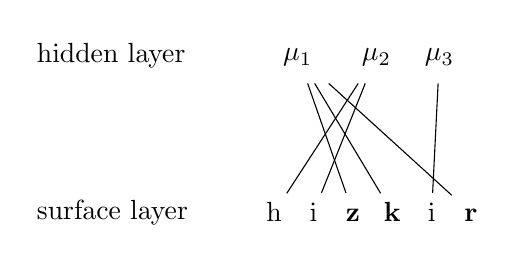
\begin{tikzpicture}[shorten >=1pt,draw=black!100]
	\def \rowtwoht{4cm}
	%\def \weightstwo{3.75cm}
	\def \rowoneht{2cm}
	%\def \weightsone{1.25cm}
	%\def \basement{0cm}
	\tikzstyle{m-node}=[text height=6pt,text centered,inner sep=2pt,minimum size=12pt]
	\tikzstyle{r-node}=[text height=6pt,text centered,inner sep=6pt,minimum size=12pt]
	\tikzstyle{d-node}=[text height=6pt,text centered,inner sep=6pt,minimum size=12pt]
	\tikzstyle{annot}=[text width=20ex]
	% labels
	\node[annot] (mtierstop) at (0cm,\rowtwoht) {hidden layer};
	\node[annot] (segtier) at (0cm,\rowoneht) {surface layer};
	%\node[annot] (mtiersbot) at (0cm,\basement) {};
	
	% hidden layer
	\node[m-node] 	(m0)	at (1.5cm,\rowoneht)		{h};
	\node[m-node] 	(m1)	at (2.0cm,\rowoneht)		{i};
	\node[m-node] 	(m2)	at (2.5cm,\rowoneht)		{\textbf{z}};
	\node[m-node] 	(m3)	at (3.0cm,\rowoneht)	 	{\textbf{k}};
	\node[m-node] 	(m4)	at (3.5cm,\rowoneht)	 	{i};
	\node[m-node] 	(m5)	at (4.0cm,\rowoneht)	 	{\textbf{r}};
	
	% reconstructed vector
	\node[r-node] 	(r0)	at (1.8cm,\rowtwoht)		{$\mu_{1}$};
	%\node[r-node] 	(r6) 	at (9.75cm,\rowoneht)   	{$r_J$};
	
	% data vector
	\node[d-node] 	(d0)	at (2.8cm,\rowtwoht)		{$\mu_{2}$};
	\node[d-node] 	(d1)	at (3.6cm,\rowtwoht)		{$\mu_{3}$};
	%\node[d-node] 	(d6) 	at (9.75cm,\basement)   	{$d_J$};
	
	\path
		(r0)	edge	node	{}	(m2)
		(r0)	edge	node	{}	(m3)
		(r0)	edge	node	{}	(m5)
		%
		(d0)	edge	node	{}	(m0)
		(d0)	edge	node	{}	(m1)
		(d1)	edge	node	{}	(m4);
	\end{tikzpicture}
	%\label{subfig:multilinear-gt-2}
%	} \hspace{2cm}
%	\subfigure[Linear approach\label{subfig:linear-2}]{
%	\begin{tikzpicture}[shorten >=1pt,draw=black!100]
%
%	\def \floor{2cm}
%	\tikzstyle{f-node}=[text height=6pt,text centered,inner sep=6pt,minimum size=15pt]
%	\tikzstyle{annot}=[text width=20ex]
%	% labels
%	\node[annot] (floorlabel) at (0cm,\floor) {surface layer};
%	
%	% surface layer
%	\node[f-node] 	(f0)	at (1.4cm,\floor)		{h};
%	\node[f-node] 	(f1)	at (1.7cm,\floor)		{i};
%	\node[f-node] 	(f2)	at (2cm,\floor)		{$|$};
%	\node[f-node] 	(f3)	at (2.3cm,\floor)		{\textbf{z}};
%	\node[f-node] 	(f4)	at (2.6 cm,\floor)	 	{\textbf{k}};
%	\node[f-node] 	(f5)	at (2.9 cm,\floor)	 	{$|$};
%	\node[f-node] 	(f6)	at (3.2 cm,\floor)	 	{i};
%	\node[f-node] 	(f7)	at (3.5 cm,\floor)	 	{$|$};
%	\node[f-node] 	(f8)	at (3.8 cm,\floor)	 	{\textbf{r}};
%	\end{tikzpicture}
%	%\label{subfig:linear-gt-2}
%	}
\label{fig:autoseg-to-bipartite}
%\caption{Two approaches to analyzing \textit{hizkir} (`he reminded'), which has three morphemes. 
%The root \textit{z.k.r} (boldface) is discontinuous. The linear (single-tier) approach is unable to connect the \textit{r} to the \textit{zk}, while the multilinear approach is able to unite discontiguous elements through external morpheme ($\mu$) nodes.}
\caption{The morphs are line up to form a vector. They are still orthogonal, and thus each still occupies its own tier.}
%: an input layer ($\mathbf{d}$), a hidden layer ($\mathbf{m}$), and an output layer
\end{mdframed}
\end{figure} 
The segmental tier would constitute the other partition. 
Since the components of a vector are orthogonal, 
we can still think of each morph in the vector of morphs as residing on its own tier.
% regarded 
%as residing on different tiers. %This would not effect the indpendence of th mo
%in order to enable this system
% Explored in linguistic theory and computationally with hand-written grammars ...
%to learn nonconcatenative morphology without supervision. 
%in a machine learning system capable of learning nonconcatenative morphology without supervision.
%During the course of development, I will explore different options for system components, e,g., the set of features,
%in order to arrive at the configuration that gives the best result for learning autosegmental morphology.  

%0. Already accepted as fact/Already proposed/hypothosized. Isolate the aspect(s) of AT that are responsible 
%for its ability to deal with nonconcatenative morphology.
%\cite{mccarthy:1981} has shown that it is the multilinear architecture of autosegmental theory that allows it to deal with
%nonconcatenative morphology. 
%In graph theoretic terms, this multilinear formalism constitutes a \emph{multipartite}, or $K$-partite, graph,
%i.e., a graph whose nodes form $K$ sets of \emph{mutually nonadjacent} nodes. That is, there are no edges between nodes of the same set, but there may be an edge betwech-Introen edges of different sets. 

%In an autosegmental representation, each tier, or morpheme, 
%is a set of mutually nonadjacent nodes, where   
%each node is a distinct bundle of phonological features.
%But note that each morpheme tier can be represented abstractly as a single node; that is, 
%its component nodes need not be represented explicitly 
%because they are given by the edges linking the morpheme to the phonological segments.
%We can thus view all the morph tiers as composing a single tier, 
%with each morpheme represented as a single node in this tier.
We will call this morph vector the \emph{hidden} \emph{layer}, 
the segmental tier the \emph{surface} \emph{layer}. The morphs 
in the hidden layer thus become \emph{hidden units}, and the phonological segments (or features or characters)
in the surface layer become \emph{surface units}.
In this way, the autosegmental multilinear framework can be 
represented as a bipartite graph.

%This bipartiteness is important because many learning algorithms are based on bipartite graphs. I will be focusing on one such algorithm called
%the Multiple Cause Mixture Model (MCMM)
%\citep{saund:94}. An MCMM is a kind of autoencoder network with a bipartite architecture. It has two layers of nodes, a reconstruction (surface) layer $R$, where it attempts to reconstruct the input feature vectors and a hidden layer whose nodes encode shared features among the input vectors. Weighted arcs link the nodes of one layer to those of the other, but there are no \emph{intra}-layer connections.



% Describe how autosegmental theory reduces to a bipartite graph. 
In an autosegmental representation, each morph tier is a complex object, consisting of a particular sequence of phonological feature matrices such as [-front,+low,-round,+syllabic]. However, phonemic symbols are often used as shorthand for
feature matrices; for example, the feature matrix [-front,+low,-round,+syllabic] can
%\begin{exe}
%\ex \[-front,+low,-round,+syllabic\]
%\end{exe}
% can 
be written as \textipa{/a/}. A sequence of feature matrices can thus be 
reduced to a sequence of alphabetic characters, each representing its own 
bundle features. For example, in figure~\ref{subfig:multilinear-gt}, 
one morph is represented as the phonemic sequence \textipa{/hi/}, which itself is a representation (an abbreviation)
of a sequence of features matrices. That is, %[+spread glottis][+front,-low,-round,+syllabic]
\begin{exe}
\ex \textipa{/hi/} \quad $\mapsto$ \quad \textipa{/}[+spread glottis][+front,-low,-round,+syllabic]\textipa{/}
\end{exe}
where 
\begin{exe} 
\ex  \label{ex:h-feats} \textipa{/h/} \quad $\mapsto$ \quad \textipa{/}[+spread glottis]\textipa{/}
\ex  \label{ex:i-feats} \textipa{/i/} \quad $\mapsto$ \quad \textipa{/}[+front,-low,-round,+syllabic]\textipa{/}
\end{exe}
%\begin{exe}
%[+spread glottis] corresponds to the /h/ and [+front,-low,-round,+syllabic] to the /i/.
When the feature matrices represented by /h/ and /i/ become linked to the first 
C and the first V, respectively, the C and V inherit the feature specifications in these matrices; in effect,
the features matrices in (\ref{ex:h-feats}) and (\ref{ex:i-feats}) \emph{become} the
feature matrices of the first C and V (respectively),
which means that /h/ and /i/ can now stand in for them also. %(respectively). 

A CV skeleton becomes a sequence of fully fledged phonemes, i.e., a phonological
form, as soon as the morphs connect to the C and V slots, whereupon on the individual Cs and Vs inherit the individual feature matrices composing the morphs and hence, in effect, take on the phonological identities
embodied by those feature matrices.  
%on the identities of the phonological elements that compose the morphs. 
Thus, just as \textipa{/hi/} and \textipa{/i/} (i.e, the feature bundles they represent) compose 
$\mu_1$ in figure~\ref{subfig:multilinear-gt}, they also compose a morphological 
unit within the segmental tier, once $\mu_1$ has linked to the appropriate C and V slots. The morphs $\mu_1$, $\mu_2$, and $\mu_3$ 
essentially \emph{cause} the segmental tier to be realized as a fully fledged 
phonological form. This observation will become especially relevant in 
section~\ref{sec:bipartite} below and in the following chapter, were we explore multiple cause mixture models (MCMMs) in depth.
% the 
%close to describing the workings of \ac{MCMM}. 

%One might thus object to the simplicity of figure~\ref{subfig:multilinear-gt}, e.g., its denoting the autosegmental morph tiers as $mu1$, etc., as though they were atomic units. But these labels are merely a form of shorthand. That is, one can generally use phonemic symbols as shorthand for
%feature matrices; e.g., the feature matrix [+back,+low, -cons] can be written as /a/
%%is a set of mutually nonadjacent nodes, where   
%each node is a bundle phonological features, e.g., [+back,+low, +syllabic]. However, one can generally use phonemic symbols as shorthand for
%feature bundles (or matrices); e.g., the feature matrix [+back,+low, +syllabic] can be written as /a/. 
%as  

Furthermore, we can think of the each C and V slot in the segmental tier as a \emph{node}.
We can also think of each morph $\mu_k$ as a node. 
%These features are mapped onto the
%C and V slots in McCarthy's segmental tier. 
 Each of these nodes is (or represents) a complex object. In particular, each C and V node
 is a matrix of features, and morph node is a \emph{sequence} of (one or more) feature matrices. Thus, a single morph node, e.g., $\mu_1$, can be associated with more than one CV node because the morph node itself \emph{is equivalent to} more than one phonological unit.  
% tassociation arcs
%fan out from a single morph morph node to meet more than one individual C and V nodes
% given morph node to 
% mapping from a morph nodes to CV nodes. 
Thus, CV node represents a phonological unit, and each morph node represents a sequence of phonological units.
Fundamentally, therefore, both represent the same type of units, namely, phonological units, and both can be expressed in terms of phonological units.
%But note that each morpheme tier can be represented abstractly as a single node; that is, 
%its component nodes need not be represented explicitly 
%because they are given by the edges linking the morpheme to the phonological segments.
%We can thus view all the morpheme tiers as composing a single tier, with each morpheme represented as a single node in this tier.
We will call the layer of  morph nodes the \emph{hidden} \emph{layer} and layer of CV nodes (i.e., the segmental tier) the \emph{surface} \emph{layer}. 
In this way, the multilinear framework of autosegmental morphology can be expressed as a bipartite graph.

%Moreover, \dots

%In graph-theoretic terms, the multilinear formalism of
%\citet{mccarthy:1981} is a %type of \emph{multipartite}
%therefore a bipartite
%graph. %This is a graph whose nodes can be partitioned into two sets whose members are \emph{mutually nonadjacent}; i.e., no two nodes within the same set are connected by an edge.
%\emph{mutually nonadjacent}, i.e., disconnected, nodes; i.e., there are no connections between nodes of the same set. %two sets such that whose defining characteristic is that no two nodes with
%nodes within the \emph{same} set are connected by an edge.
%figure~\ref{fig:gt-bipartite}, for example, shows a \emph{bipartite}
%graph, i.e., a graph with two such partitions, namely the sets $M$
%and $R$ in this case.
%Within each set, or \emph{layer}, all nodes are independent; there are no
%intra-layer connections. The only connections are 
%between nodes of different sets.



%This bipartiteness is important because many learning algorithms are based on bipartite graphs. I will be focusing on one such algorithm called
%the Multiple Cause Mixture Model (MCMM)
%\citep{saund:94}. An MCMM is a kind of autoencoder network with a bipartite architecture. It has two layers of nodes, a reconstruction (surface) layer $R$, where it attempts to reconstruct the input feature vectors, and a hidden layer whose nodes encode shared features among the input vectors. Weighted arcs link the nodes of one layer to those of the other, but there are no \emph{intra}-layer connections.

% Hebrew morphology, both its non-concatenative and concatenative components. 
%In a multilinear framework, concatenative morphology is just a special case of non-concatenative morphology. There is no fundamental difference between them.
\section{An MCMM is a Bipartite Graph}\label{sec:mcmm-bipartite}
%An MCMM, as it turns out, is a special case of a bipartite graph. Indeed,

% itself be a simple MCMM. %precisely the architecture of an MCMM.
%To sum up, bipartite graphs possess the properties nonlinerarity and nonsequentiality. 
%Because MCMMs are bipartite graphs, and bipartite graphs are both nonlinear and nonsequential, 
%MCMMs must themselves be nonlinear and nonsequential, which makes MCMMs well-suited for modeling
%non-concatenative morphology.

%As it turns out, 
% (figure~\ref{subfig:nonlinear}). 
%\section{Conclusion}
%\label{sec:graph-concl}

%That is, because of its bipartite properties, an MCMM provides a sound framework in which to implement autosegmental morphology, or at least the components of autosegmental morphology that address non-concatenative morphology.
%An MCMM
%%, as it turns out, 
%is clearly a bipartite graph. 
We will discuss the architecture of MCMMs in detail in the following chapter. 
We will see  that has two
layers of nodes, a hidden layer and a
surface layer---corresponding, respectively, to $M$ and $R$ in
figure~\ref{fig:gt-bipartite}. Moreover, there are no intra-layer connections in
MCMM; the only connections inter-layer, between $M$ and $R$ nodes.
%For the moment, suffice it to say that
%the graph
%figure~\ref{fig:gt-bipartite} could itself be a diagram of an MCMM. 
%Let us thus stipulate for the moment that MCMMs are bipartite graphs. %precisely the architecture of an MCMM.
%To sum up, bipartite graphs possess the properties nonlinerarity and nonsequentiality. 
Because MCMMs are bipartite graphs, therefore, and because bipartite graphs are both nonlinear and nonsequential, 
MCMMs must themselves be nonlinear and nonsequential. This makes them well-suited for modeling
nonconcatenative morphology, as discussed in chapter~\ref{ch:lit-review}.


%Because a bipartite graph satisfies nonlinearity and nonsequentiality,  
%we can reformulate the morph tiers and the
%segmental tier in figure~\ref{subfig:nonlinear-gt} as the sets $M$ and
%$R$, respectively, in figure~\ref{fig:gt-bipartite} This satisfies nonlinearity. As nonsequentiality, note that each node in $M$ represents a morpheme (or
%morpheme tier), and, by the definition of \emph{bipartite}, the nodes
%within $M$ are independent and thus orthogonal.
%
%An MCMM %(section~\ref{sec:mcmm}) 
%is well-suited to learn 
%non-concatenative morphology because it is bipartite graph. 
%It has two
%\emph{layers} (equivalently, sets) of nodes, a hidden layer and a
%surface layer---corresponding, respectively, to $M$ and $R$ in
%figure~\ref{fig:gt-bipartite}. There are no intra-layer connections in an
%MCMM, only connections between layers.

In subsequent chapters, we will refer to an MCMM's partitions as
\emph{vectors}, i.e., vectors of nodes, and use matrix and vector notation to
describe the components of an MCMM:
Uppercase boldface letters will denote matrices,%(e.g., $\mathbf{M}$),
lowercase boldface letters will denote vectors,
% and matrix rows or columns, 
%(e.g., $\mathbf{m}_i$),
and italicized lowercase letters will refer to the individual elements
of vectors and matrices. % (e.g., $m_{ik}$).
For example, $m_{i,k}$ is the $k$th %$k^{\text{th}}$ 
element in the vector
$\mathbf{m}_i$, which is the $i$th
%$i^{\text{th}}$ 
row in the $I \times K$ matrix
$\mathbf{M}$. Thus, we will henceforth write the $M$ and $R$ in
figure~\ref{fig:gt-bipartite} as $\mathbf{m}$ and $\mathbf{r}$,
respectively (or $\mathbf{m}_i$ and $\mathbf{r}_i$, where $i$ is the
index of the $i$th
%$i^{\text{th}}$ 
word).

\section{Summary}\label{sec:graph-concl}
The essence of autosegmental morphology can be expressed in terms of nonlinearity
and nonsequentiality. These two properties are equivalent to the properties of a bipartite graph. Thus, the autosegmental formalism
reduces to a bipartite graph. %We have just seen that  MCMM is practically the golden retriever of bipartite graphs.
Furthermore, an MCMM is a bipartite graph, in particular, a bipartite graphical learning model. The autosegmental formalism and the MCMM are thus related to
each other through their shared bipartiteness, and thus an MCMM can serve as a vehicle for realizing autosegmental morphology in a computational process. In the next chapter, we focus on the MCMM itself.
%establishes a  
%an MCMM is a bipartite graph, 
%and that, consequently, it is compatible, so to  speak, with autosegmental morphology.
%itself has a bipartite architecture, which is to say that it can be represented as and thought of as a bipartite graph without information loss.  essentially bipartite in its architecture, and that it ; we will see that the autosegmental framework is essentially a bipartite graph. We shall then observe in section~\ref{sec:bipartite} that an \ac{MCMM} is itself a bipartite graph, and that autosegmental morphology and \ac{MCMM}s have the same graphical properties. 
%A bipartite graph suffices
%%we do not need many partitions 
%to capture the essential properties of McCarthy's autosegmental
%framework,
%and that, consequently, it is compatible with autosegmental morphology. 
%In other words, an MCMM can serve as a
%a computational ``wrapper," so to speak, for McCarthy's autosegmental theory, a 
%means whereby it can be specially packaged for use in a machine learning system. 
%AND NOW, ONWARD to chapter~\ref{ch:MCMM}, in which we shall discuss MCMM in greater depth. % Graph-Theoretic Foundation
\chapter{The Multiple Cause Mixture Model}
\label{ch:MCMM}

\section{Introduction}
\label{sec:mcmm:intro}
Multimorph, as an unsupervised learning system, must be 
driven by an unsupervised learning algorithm, that is, 
a procedure for inducing categories from raw, unlabeled data.
%This thesis's preceding chapters have established the basic requirements for Multimorph's learning
%algorithm.
This chapter focuses on Multimorph's core learning algorithm, the Multiple Cause Mixture Model (MCMM). In particular, it motivates the choice of the MCMM \citep{saund:94}. In doing so, it explains the nature, structure, and function of MCMMs, and why an MCMM is an appropriate learning mechanism for Multimorph. 

This chapter is a culmination of the argumentation of the preceding three chapters. 
In chapters~\ref{ch:intro} and \ref{ch:lit-review}, we saw that it was precisely 
the set of \emph{nonlinear-nonsequential} models that were capable of representing 
nonconcatenative morphological structure, and that it was the properties \emph{nonlinearity}
and \emph{nonsequentiality} that give rise to this capacity. Furthermore, we in 
chapter~\ref{ch:graph} that bipartite graphs (or bipartite graphical algorithms) were a subset of NLNS algorithms. In fact, the bipartite structure of such graphs turned out to be a particularly coherent way to capture nonlinearity and nonsequentiality (REF).
%ince its relationship to the autosegmental architecture is straightforward.  
%demonstrated the equivalence between nonlinearity and 
%nonsequentiality and the mathematical properties of 
%bipartite graphs, thereby showing that bipartite graphs are 
%intrinsically nonlinear and nonsequential. It follows that bipartite graphs are 
%well-suited to represent nonconcatenative structure, and moreover, that bipartite graphical learning models are thus intrinsically well-suited to serve as learning algorithm for a ULM system. 
The present chapter homes in on a particular kind of bipartite learning algorithm, namely the MCMM. The preceding chapters provide the chain of reasoning that leads to our choice of the MCMM.

%For Multimorph, I chose a particular kind of bipartite learning model called the Multiple Cause Mixture Model (MCMM), developed by \citet{saund:94}.

%MCMMs are conducive to ULM, particularly to the UL of non-concatenative morphology, mainly because they are bipartite graphs, since it is their bipartiteness that makes them nonlinear and nonsequential. The bipartiteness of MCMMs is evident in Section~\ref{sec:architecture} (see in particular figure~\ref{fig:mcmm}), which elucidates the architecture
%of an MCMM. But while their bipartiteness is most significant for our purposes, MCMMs have other attractive properties. [which we shall discuss in this chapter.] For example, an MCMM is neither sum nor a product of experts, 

%In this chapter, therefore, we thus present a particular bipartite graphical model,  as Multimorph's core learning algorithm. In particular, I chose the bipartite graphical model known as the MCMM.
The chapter is organized as follows: Section first lays out the key components of an MCMM's structure, i.e., the attributes that all MCMMs share. Section~\ref{sec:context} then proceeds to place MCMMs in a larger of unsupervised learning algorithms, demonstrating 
%In doing so, it will break down the structure of MCMMs, demonstrating 
the similarities and differences between MCMMs and other types of learning algorithms such as Restricted Boltzmann Machines (RBM) and Latent Dirichlet Allocation (LDA). Section~\ref{mixing-function} focuses a particularly important component of an MCMM, namely its \emph{mixing function}, which is a type of activation function, i.e., a function that determines the activities of nodes in neural networks.  
%Section~\ref{sec:architecture} describes the architecture of MCMMs. 
Finally, section~\ref{sec:mcmm-learning} discusses the means by which MCMMs learns, paying particular attention to Multimorph's MCMM.

%demonstrates the bipartite nature of an MCMM; compare figure~\ref{fig:mcmm} in section~\ref{sec:architecture} to the canonical bipartite structure shown in figure \ref{fig:gt-bipartite} in chapter~\ref{ch:graph}. whose bipartiteness becomes clearly evident in section~\ref{sec:architecture} Section~\ref{sec:architecture} also breaks the architecture of an MCMM, describing its basic components and how they relate to each other. hen delves deeper into the nature the MCMM, comparing and contrasting it to related learning algorithms, such as the Restricted Boltzmann Machine (RBM). Finally, section~\ref{sec:mcmm-learning} discusses the particular means by which Multimorph's MCMM learns.

% learning process itself in detail. The following section then describesSection~ fact that will become plainly evident in section~{sec:architecture}  reasoning to motivate the use of bipartite graphical learning model, specifically the MCMM, as Multimorph's algorithm.  takes this this line of argumentation to its logical conclusion i  a bipartite graphical model, namely the MCMM, tononconcatenative morphology, and thus a bipartite graphical learning algorithm is going to be at least furthermore, a bipartite archict
%In this chapter, we pre 
%From  that bipartite graphs intrinsically nonlinear and nonsequential, and that bipartite graphical learning models are 
%Thus, a bipartite architecture implies both nonlinearity and nonsequentiality and hence a capacity for representing both nonconcatenative and concatenative morphological structure. 
%
%Proposition x thus motivates the choice of bipartite graphical model to serve as Multimorph's learning suitable for learning  have the capacity to represent both nonconcatenative and concatentative morphological struThis brings us to the primary concern of the present the chapter: the choice of Multimorph's core learning algorithm. Motivated by the results of the previous chaptersparticular, the preceding chapters motivate and thus capable of representing nonconcatenative morphology. All of this is Multimorph's learning algorithm

%I chose the Multiple Cause 
%Mixture Model (MCMM) proposed by \citet{saund:94} to fill this role. The present chapter motivates this decision, and in doing so, provides a detailed exposition of the MCMM. Section~\ref{sec:architecture} first provides an overview of an MCMM's architecture, i.e., a description of its major components and the relationships between these components. Section~\ref{sec:architecture} then delves deeper into the nature the MCMM, comparing and contrasting it to related learning algorithms, such as the Restricted Boltzmann Machine (RBM).   comparing it to other including a description of their architecture in detail. describes the will be motivated in the present present chapter.  The present chapter will describe   primary objective of this chapter  motivate this decision; first of all, it will show in section~{sec:architecture}that it is a bipartite graph and thus qualifies as a nonlinear-nonsequential algorithm. \citet{saund:94}  nonlinear-nonsequential models are argued that nonlinearity and nonsequentiality were essential properties learning nonconcatenative
%morphology must be   
%Multimorph's learning algorithm is an instance of an Multiple Cause 
%Mixture Model (MCMM) proposed by \citet{saund:94}, and thus MCMMs
%is a major focus of this chapter.

%By \emph{model}, 
%we mean a set of assumptions about how the world works. Where Multimorph is concerned, 
%the ``world" is the morphology of natural languages, which, significantly, includes \emph{non-concatenative} morphology. 
%autosegmental morphology \citep{mccarthy:1981}. 
%In chapter~\ref{ch:graph}, we argued
%that in order
%for a model to be able to deal with nonconcatenative morphology,
% it must be both \textbf{nonlinear} \textbf{and}
% \textbf{nonsequential},
% i.e., satisfy both the \textsc{Nonlinearity} criterion and the \textbf{Nonsequentiality} criterion; 
% see definitions (\ref{def:nl}) and (\ref{def:ns}) and 
% proposition (\ref{prop:nlns}). We also saw in chapter~\ref{ch:graph} that these two conditions are equivalent to the two parts of the definition of biparteness. In particular, \dots.
 



% Therefore, if a model is a bipartite graphical model, then it is both nonlinear and nonsequential, which means
% that it has the capacity to model nonconcatenative morphology:
%  \begin{proposition}
%% In order for a model to be able to handle non-concatenative morphology, it must be a bipartite graph.
%% \end{proposition}
%  \label{prop:bipartite}
%If a model is a bipartite graph, it can handle nonconcatenative morphology. Moreover, if it can handle nonconcatenative morphology, it can handle concatenative morphology.
% \end{proposition}
 
%if a model is a bipartite graph, 
%it has the capacity to deal with nonconcatenative morphology.
%% of morphology are treated as the same basic phenomenon; the capacity to model nonconcatenative morphology is actually the more general capacity, since a concatenative process is essentially a nonconcatenative process with zero interdigitation. 
%That is, if there were such a thing as a ``morph discontiguity factor,'' that is, a some sort of measure of the degree to which the phonemes of different morphs tend to be interleaved (i.e., the tendency of morphs to be discontinuous), 
%%separation between phonemes of the same morpheme discontiguous the  phonemes of the same morph separated by intervening phonemes (from another morph) by those of other morphs), 
%then this metric would be zero for ``strictly concatenative'' morphological processes, and some number greater than zero for ``nonconcatenative" ones. The point is that there no categorical difference between concatenative and nonconcatenative processes. Fundamentally, the two type of processes are in fact one and the same  process.  Thus, the capacity to model noncatenative morphology implies the capacity to model concatenative morphology. 
%Noncatenative morphology can thus be regarded as the more general case.
% \begin{proposition}
%% In order for a model to be able to handle non-concatenative morphology, it must be a bipartite graph.
%% \end{proposition}
%  \label{prop:bipartite}
%If a model is a bipartite graph, it can handle nonconcatenative morphology. Moreover, if it can handle nonconcatenative morphology, it can handle concatenative morphology.
% \end{proposition}

 %call for a bipartite graph, since they are essentially equivalent to
% The Multiple Cause Mixture Model (MCMM) is a general 
% framework for unsupervised learning developed by \cite{saund:94}. 
% Section~\ref{sec:architecture} in this chapter will describe the architecture 
% of an MCMM, i.e., its key components and the relationships between these 
% components. It will become clear in this section that MCMMs are bipartite 
% graphs and thus, by proposition~\ref{prop:bipartite}, an MCMM is capable 
% of learning nonconcatenative morphology. 
 %serve as Multimorph's core learning framework.
 %  In this chapter, we shall first demonstrate an MCMM qualifies as a bipartite graph.  
%In addition to demonstrating the bipartite \emph{bona fides} of MCMMs, this chapter will, in section~\ref{sec:architecture}, discuss the architecture of an \ac{MCMM},
%i.e., is key components and the relationships between these components. 
%This chapter will also, in 
%sections~\ref{sec:mixing-function} and \ref{sec:mcmm-learning}, describe the process whereby
%an \ac{MCMM} learns. 

\section{Basic MCMM Architecture}
\label{sec:architecture}

In \citet{saund:94}, the term \emph{multiple cause mixture model} does to refer a single, 
specific algorithm, but rather to a family of algorithms, i.e., a general framework for unsupervised learning.  Since MCMMs constitute a definite category of algorithms, all MCMMs share certain key attributes. %These components and the relationships between them are the subject of this section. 
These attributes are in large part the subject of this section. 
%These are described in section~\ref{sec:architecture}. 
%so every MCMM must have certain key
%key attributes in order to qualify as an MCMM. 
%For instance, all MCMMs bipartite graphs, as illustrated in figure~\ref{fig:mcmm}. That is, for instance, 
%However, there is also room for variation among MCMMs. In particular, MCMMs may vary in their \emph{mixing function}.
%
%All MCMMs are 
%All have a the same in certain crucial ways.
%All share g There can thus be different kinds of MCMMs. 
%does not refer to a single, fully specified algorithm, but rather to a family of algorithms, 
%i.e., a \emph{framework} consisting of components that are only loosely rather fully 
%specified, thus allowing for a range of options as long as they satisfy certain criteria. 
%For example, one essential component of an MCMM is the \emph{mixing function}.


%\begin{tikzpicture}[scale=1.25]%,cap=round,>=latex]
%\coordinate [label=left:$A$] (A) at (-2cm,-1.cm);
%\coordinate [label=right:$C$] (C) at (2.2cm,-1.0cm);
%\coordinate [label=above:$B$] (B) at (1cm,1.0cm);
%\draw (A) -- node[sloped,above] {c} (B) -- node[sloped,above,] {a} (C) -- node[below] {b} (A);
%\draw[dashed] (B) -- (A-|B) ;
%\end{tikzpicture}

%\begin{figure}[ht]
%\begin{tikzpicture}
%\node[draw,circle] (A) at (90:3) {A};
%\node[draw,circle] (B) at (210:3) {B};
%\node[draw,circle] (C) at (330:3) {C};
%\draw[latex'-latex',double] (A) -- node[label=150:A-B,label=330:B-A] {} (B);
%\draw[latex'-latex',double] (A) -- node[label=30:A-C,label=210:C-A] {} (C);
%\draw[latex'-latex',double] (B) -- node[label=90:B-C,label=270:C-B] {} (C);
%\end{tikzpicture}
%\label{fig:alg-types}
%\caption{Relationship between the terms \emph{autoencoder}, \emph{MCMM}, and \emph{RBM}}
%\end{figure}

An MCMM is a graphical model consisting of two layers of nodes (or units): a layer 
of \emph{surface} or \emph{visible} units 
and a layer of \emph{hidden} units. 
This is illustrated in figure~\ref{fig:mcmm}, where $\mathbf{m}$ 
is the vector of hidden units. The vector $\mathbf{x}_i$ is the 
original vector of surface units\footnote{Saund uses $\mathbf{d}$ 
rather than $\mathbf{x}$ to denote this vector}; it is the observed, 
real-world data. The vector $\mathbf{r}_i$ is the ``working" 
reconstruction of $\mathbf{x}_i$. It is dynamic; 
it evolves as the learning process progresses, hopefully 
becoming more and more similar to $\mathbf{x}_i$. 
This is the essence of the learning process and will be 
discussed more fully in section~\ref{sec:mcmm-learning}).
that $\mathbf{x}_i$ is not directly connected to either $\mathbf{r}_i$ 
or $\mathbf{m}_i$. It is not an integrated component of the graphical 
model. Its role is to as a target for the reconstruction $\mathbf{r}_i$. 
The goal of the system as a learning model is to get $\mathbf{r}_i$ to 
match $\mathbf{x}_i$, i.e., to reconstruct $\mathbf{x}_i$ in 
$\mathbf{r}_i$ (as discussed in section~\ref{sec:mcmm-learning}).
% shall discuss this reconstruction process in more detail in section REF.

\begin{figure}[htb]
\begin{center}
%\small
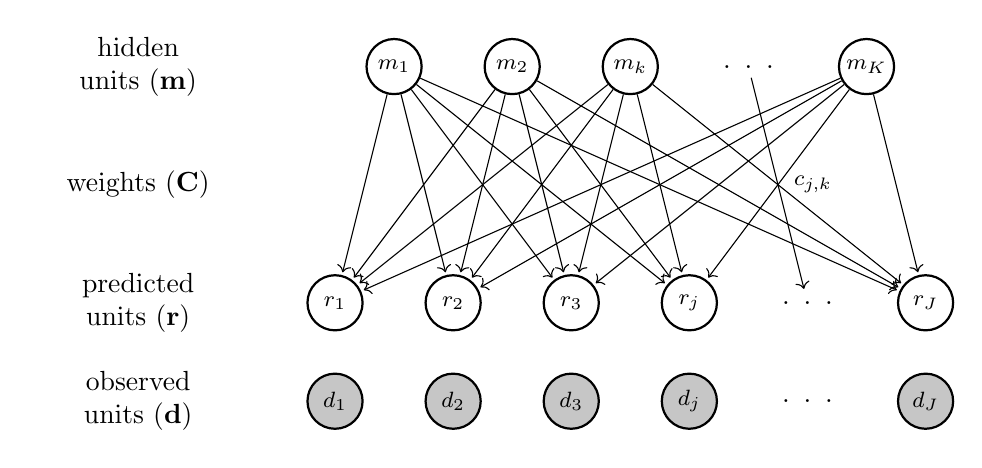
\begin{tikzpicture}[shorten >=1pt,->,draw=black!100]
	\def \rowtwoht{4.25cm}
	\def \weightlevel{2.75cm}
	\def \rowoneht{1.25cm}
	\def \basement{0cm}
	\tikzstyle{m-node}=[circle,draw=black!100,thick,inner sep=0pt,minimum size=7mm]
	\tikzstyle{r-node}=[circle,draw=black!100,thick,inner sep=0pt,minimum size=7mm]
	\tikzstyle{d-node}=[circle,draw=black!100,fill=gray!45,thick,inner sep=0pt,minimum size=7mm]
	\tikzstyle{dots}=[text width=5ex, text centered]
	\tikzstyle{annot}=[text width=17ex, text centered]
	% labels
	\node[annot] (hidden-layer) at (0cm,\rowtwoht) {hidden units ($\mathbf{m}$)};
	\node[annot] (weights) at (0cm,\weightlevel) {weights ($\mathbf{C}$)};
	\node[annot] (r-layer) at (0cm,\rowoneht) {predicted units ($\mathbf{r}$)};
	\node[annot] (d-layer) at (0cm,\basement) {observed units ($\mathbf{d}$)};
	
	\node[dots] 	(m3)	at (7.75cm,\rowtwoht)	 	{. . .};
	\node[dots] 	(r4) 	at (8.5cm,\rowoneht)   		{. . .};
	\node[dots] 	(d4) 	at (8.5cm,\basement)   		{. . .};
	
	\footnotesize
	% hidden layer
	\node[m-node] 	(m0)	at (3.25cm,\rowtwoht)		{$m_1$};
	\node[m-node] 	(m1)	at (4.75cm,\rowtwoht)		{$m_2$};
	\node[m-node] 	(m2)	at (6.25cm,\rowtwoht)	 	{$m_k$};
	\node[m-node] 	(m4)	at (9.25cm,\rowtwoht)	 	{$m_K$};
	
	% reconstructed vector
	\node[r-node] 	(r0)	at (2.5cm,\rowoneht)		{$r_1$};
	\node[r-node] 	(r1)	at (4cm,\rowoneht)		{$r_2$};
	\node[r-node] 	(r2)	at (5.5cm,\rowoneht)	 	{$r_3$};
	\node[r-node] 	(r3)	at (7cm,\rowoneht) 		{$r_j$};
	\node[r-node] 	(r5) 	at (10cm,\rowoneht)   		{$r_J$};
	%\node[r-node] 	(r6) 	at (9.75cm,\rowoneht)   	{$r_J$};
	
	% data vector
	\node[d-node] 	(d0)	at (2.5cm,\basement)		{$d_1$};
	\node[d-node] 	(d1)	at (4cm,\basement)		{$d_2$};
	\node[d-node] 	(d2)	at (5.5cm,\basement)	 	{$d_3$};
	\node[d-node] 	(d3)	at (7cm,\basement) 		{$d_j$};
	\node[d-node] 	(d5) 	at (10cm,\basement)   		{$d_J$};
	%\node[d-node] 	(d6) 	at (9.75cm,\basement)   	{$d_J$};
	
	\path 
		(m0)	edge	node	{}	(r0)
		(m0)	edge	node	{}	(r1)
		(m0)	edge	node	{}	(r2)
		(m0)	edge	node	{}	(r3)
		(m0)	edge	node	{}	(r5)
		
		(m1)	edge	node	{}	(r0)
		(m1)	edge	node	{}	(r1)
		(m1)	edge	node	{}	(r2)
		(m1)	edge	node	{}	(r3)
		(m1)	edge	node	{}	(r5)
		
		(m2)	edge	node	{}	(r0)
		(m2)	edge	node	{}	(r1)
		(m2)	edge	node	{}	(r2)
		(m2)	edge	node	{}	(r3)
		(m2)	edge	node	{}	(r5)
		(m3)	edge	node[right=1mm]	{$c_{j,k}$}	(r4)
		%	
		(m4)	edge	node	{}	(r0)
		(m4)	edge	node	{}	(r1)
		(m4)	edge	node	{}	(r2)
		(m4)	edge	node	{}	(r3)
		(m4)	edge	node	{}	(r5);
		
\end{tikzpicture}
\end{center}
\caption{Architecture of a Multiple Cause Mixture Model (MCMM)} 
\label{fig:mcmm}
\end{figure}

'
The vector $\mathbf{x}_i$ is but one of the $I$ rows the constitute the whole 
input corpus, the data matrix $X$. Each row contains $J$ columns. Similarly, 
$\mathbf{r}_i$, the reconstruction of $\mathbf{x}_i$, is the $i$th row in the 
$I \times J$ matrix $\mathbf{R}$. The subscript on the hidden-unit vector 
$\mathbf{m}_i$ indicates that it is related to $\mathbf{x}_i$ and $\mathbf{r}_i$. 
Each $J$ corresponds to a particular surface unit, i.e., feature. 
The hidden-unit vector is a row in the larger $I \times K$ matrix 
$\mathbf{M}$. Each of $\mathbf{M}$'s $K$ corresponds to a particular 
\emph{cluster}, and thus, the activity of each $m_{i,k}$ indicates whether the $i$th 
datapoint $\mathbf{x}_i$ (via its reconstruction $\mathbf{r}_i$) is a member of the 
$k$th cluster.  columns contains $I$, each the particular vector of hidden causes for 
the $i$th surface vector. $\mathbf{}$ has $K$ columns.

% is compared. 
%
%the vector of surface units; however, t
%The vector $\mathbf{x}_i$ is the original data vector, i.e., the original surface units
%
%Saund describes the hidden units in
%$\mathbf{m}_i$ as \textit{causes}; that is, the hidden units in an MCMM are presumed to hidden causes behind the particular arrangement of \textsc{on} and \textsc{off}) units in the original data vector $\mathbf{x}_i$. 
%
%\textsc{on} surface vectors
The hidden units are connected to surface units by a matrix of weights $\mathbf{C}$. 
Each individual arc $c_{j,k}$ has a value in the interval $[0,1]$. This value 
represents the weight on the connection between $m_{i,k}$ and $r_{i,j}$.
Each node, i.e., each hidden unit and each surface unit, has an activity value in $[0,1]$ that
indicates whether it is \textsc{on} (active) or \textsc{off} (inactive).
The activity of $r_{i,j}$ is determined by a \emph{mixing function}, which takes as inputs the 
hidden-unit activities $\mathbf{m}$ and their respective weights $\mathbf{c}_j$
(section~\ref{sec:mixing-function}).



\section{Relationship to Other Unsupervised Learning Frameworks}
\label{sec:context}

In this section, we relate multiple cause mixture models to other frameworks for unsupervised learning. 
Multiple cause mixture models simultaneously belong to two distinct unsupervised-learning contexts. 
On the one hand, they are neural networks, or, more specifically,\emph{autoencoders} \citep{dayan-and-zemel:95}, 
i.e., neural networks that learn without learning. On the other hand, the name 
\emph{multiple cause mixture model} 
contains the term \emph{mixture model}, which itself denotes a large class of unsupervised learning models. 
This section is therefore divided into two subsections: First, section~\ref{sec:autoencoders} considers MCMMs as neural networks, i.e., autoencoders, using neural-network terms to relate them to other autoencoders. Second, Section~\ref{sec:autoencoders} then considers MCMMs from a \emph{mixture-model} perspective, discussing their relationship to standard mixture models as well as \emph{mixed-membership} (or \emph{admixture}) models. 

%neural-network context.  them to other autoeneural network context. Second, section~\ref{sec:autoencoders} places perspective, i.e., in which case they can be described as autoencoders and compared to other instances of the autoencoder approach to learning. This is what we do in \ref{sec:autoencoders} i.e., a neural-network used for unsupervised learning.  in a  to three other learning frameworks: the classical autoencoder, the Restricted Boltzman Machine (RBM), and Latent Dirichlet Analysis (LDA). MCMMs, classical autoencoders, and Restrict Boltzmann Machines all belong to the (general) autoencoder (or unsupervised neural-network) family and thus closely related both in form and function. This LDA is not a neural-network approach, but it is similar to the MCMM in its intended purpose, namely to find multiple latent causes for single data instances.

\subsection{sec:autoencoders}
\label{sec:autoencoders}
% So-and-so classifies Saund's MCMM as a kind of autoencoder. 
%He considered a form of autoencoder network in which the hidden units signal features and the hidden-output weights describethe way in which  features generate predictions  of the inputs. 
\citet[][p. 2]{dayan-and-zemel:95} describe the MCMM as a ``form of autoencoder network.'' 
They are using the term \emph{autoencoder} in a general sense, as a class that encompasses several subtypes.  
In this general sense, an \emph{autoencoder} is any unsupervised graphical algorithm that
 learns a compressed encoding of its input data. 
% The compressed encoding from which the original can be generated, or \emph{reconstructed} which through a \emph{generative} process, i.e., a process of learning to generate its input data. To do this, it must construct an internal theory, so to speak, of its input data's structure. This theory takes the form of a compressed encoding of the input data, and in particular, a compressed encoding from which the original data can be generated, or \emph{reconstructed}.  
The learning process is essentially one of trial and error; the autoencoder iteratively tests and revises its encoding.  
%thereby improving it with each iteration. The autoencoder tests the suitability of a working encoding through \emph{reconstruction}, i.e., by attempting to recover or reconstruct the original data from the working encoding.
%Thus, at the beginning of each iteration, the autoencoder has 
The autoencoder begins each iteration with a working encoding of the input data. It tests the fitness of the encoding by attempting reconstruct each input data vector from its encoded form and measuring the \emph{reconstruction error}, i.e., the discrepancy between the reconstructed and original data vectors.  It then makes adjustments to its encoding to reduce this error, yielding a slightly improved encoding for the next iteration. 
%These adjustments, which mark the end of the current iteration, should result in a slightly better internal representation for next iteration.  

\subsubsection{Classical Autoencoder}
\label{sec:classical-auto}
%Whereas the MCMM has two layers of nodes ($\textbf{m}$ and $\textbf{r}$), 
 The ``classical'' autoencoder,
shown in figure~\ref{fig:autoencoder} has three layers (or vectors) of nodes:
%, as 
%illustrated in
%in figure~\ref{fig:autoencoder}. 
\begin{enumerate}
\item The \textbf{input} vector $\textbf{d}$
\item The \textbf{hidden} vector $\textbf{m}$
\item The \textbf{output} vector \textbf{reconstruction} layer $\textbf{r}$ 
\end{enumerate}

 Each of these vectors has a counterpart in an MCMM: \textbf{input} vector $\textbf{d}$, $\textbf{m}$, and $\textbf{r}$ vectors are analogous to the vectors of the same name in the MCMM diagram in figure \ref{fig:mcmm}.
However, there are important differences between these two types of autoencoders. The main differences pertain to form (or general architecture), node activation, i.e., the means of computing node activities, and the \emph{optimization procedure}, i.e., method for  minimizing the model's error.

\paragraph{Form.} 
In an MCMM, 
%the oriThe most conspicuous difference is that MCMMs bipartite graph, having just two layers of nodes, namely \textbf{m}$ and \textbf{r}$. Recall that in an MCMM, 
the original data vectors $\textbf{d}$ is actually not part of the graph itself, since it is not connected by weights to either  $\textbf{m}$ or  $\textbf{r}$. In a classical autoencoder, by contrast
%namely the original data vector $\textbf{d}$, the hidden-node vector $\textbf{m}$, and reconstruction vector $\textbf{r}$. These vectors are also present in the MCMM in \ref{fig:mcmm}. One key difference between an MCMM and a classical autoencoder, however, is that the the original data vector 
%$\textbf{d}$ is not a true layer in MCMM, since there are no connecting 
%weights weights between it and $\textbf{m}$ or $\textbf{r}$. This is not 
%the case in a classical encoder, where 
$\textbf{d}$ functions as the network's 
\textit{input layer}. Each input vector enters the network at $\textbf{d}$, is compressed 
at $\textbf{m}$, and reconstructed at $\textbf{r}$. Because there are three layers 
of nodes in an autoencoder, there must be two layers of weights, labeled 
$\textbf{A}$ and $\textbf{B}$ 
in \ref{fig:autoencoder}. The reconstruction error is computed at $\textbf{r}$, and the appropriate updates are 
\emph{backpropagated} to the $\textbf{B}$ and then $\textbf{A}$ weights.

%Because an MCMM has no distinct input layer, it is not a directed graph in the same way a 
%that classical autoencoder is a directed graph\footnote{There is a sort of conceptional directionality in an MCMM in that hidden nodes are regarded as ``causing'' the surface units' activities. } 
An MCMM has no designated input layer. The classical autoencoder, by contrast, has distinct input and output layers. Classical autoencoders thus function as a supervised feed-forward neural network. In fact, the only difference between a classical autoencoder and a supervised feed-forward network is that a classical autoencoder's target vectors are its input vectors.

\paragraph{Node Activation.} In a classical autoencoder, the activity of each node 
both in the hidden layer $\textbf{m}$ and the reconstruction layer $\textbf{r}$ is 
computed as a \emph{sigmoidal weighted sum}, which is the composition of the 
composition of a linear weighted sum and the nonlinear sigmoid function $\sigma$ \eqref{eq:sig}. 
The latter maps any real number (no matter how large or small) to a number within $[0,1]$.
The former is the inner product of the preceding layer's activities and the 
weight vector connecting preceding layer to the current node in the 
current layer, as in \eqref{eq:sum-m} and \eqref{eq:sum-r}.
%composition of the sigmoid function $S$ and the function $t_{i,j}$, 
%which computes a weighted sum, i.e., the inner product of the cluster-activity 
%vector $\mathbf{m}_i$ and the weight vector $\mathbf{c}_j$:

	\begin{equation} %\label{eq:sigws}
	\label{eq:sig}
	r_{i,j} =\sigma(t_{i,j}) = \frac{1}{1 + e^{-t_{i,j}}} 
	%\quad %\\   %\qquad \text{where} \quad
	%\label{eq:ws}
	\end{equation} %\label{eq:sigws}
	
	\begin{align} %\label{eq:sigws}
	\label{eq:sig-m}
	m_{i,k} =\sigma(t_{i,k}) &= \frac{1}{1 + e^{-t_{i,k}}} \\
	\label{eq:sum-r}
	\text{where} \quad t_{i,k} &= \sum_{j} x_{i,j} a_{k,j}  
	\end{align}
	
	\begin{align} %\label{eq:sigws}
	\label{eq:sig-r}
	r_{i,j} =\sigma(t_{i,j}) &= \frac{1}{1 + e^{-t_{i,j}}} \\ %\\   %\qquad \text{where} \quad
	%\label{eq:ws}
	\label{eq:sum-r}
	\text{where} \quad t_{i,j} &= \sum_{k} m_{i,k} b_{k,j} 
	\end{align}
	
For example, to compute the activity of the hidden node $m_{i,4}$ (i.e., $k = 4$), 
we would first compute the sum $\sum_{j} x_{i,j} a_{4,j}$
%, which is the equivalent to the inner product \textbf{x}_i \cdot \textbf{c}^{T}_4$ 
and then feed the result to the sigmoid function. For nodes in the reconstruction 
layer $\textbf{r}$, the input activities are hidden-node activities, and the weights 
are a particular column in the $\textbf{B}$ matrix. Thus, for node, say, 
$r_{i,6}$ (i.e., $j=6$), the summation becomes
%we would sum over the $K$ hidden-unit activities (each multiplied by its respective weight in 
%$\textbf{b}^{T}_{6}$: 
$\sum_{k} m_{i,k} b_{k,6}$.  That is, we sum over the $K$ hidden-unit activities, with each activity multiplied by its respective weight in the column (or row?) $\textbf{B}_{:,6}$). 
We again feed the sum to the sigmoid function, as we do for every node. 
The sigmoid function keeps node activities in the interval $[0,1]$.
%$\textbf{b}^{T}_{6}
% we in the reconstruction vector, specifically The latter takes the output of the linear sum, which could be any real number, possibly much less than 0 or much greater than 1, and maps it onto a number in $[0,1]$.

The sigmoidal weighted sum is a standard activation function in neural networks, 
but it is not the only way to compute the activity of a node. Any activation function, to borrow
the analogy of \citet{saund:94}, is essentially a voting rule, i.e.,  a ``policy'' for combining the node activities of one layer to yield an activity of a particular node in next/other layer. In graphical models, node activities are generally weighted, and so each vote is actually $h_{k} w_{k,j} $, where $h_{k}$ is a node activity, and $w_{k,j}$ is its weight. 

The weighted sum $\sum_{k} h_{k} w_{k,j}$ is one way of combining a set of such votes to yield a single output. The output of the weighted sum, however, can be any real number, as it grows (and shrinks) in direct proportion to the quantity and sizes of its input values. Since most applications require that node activities stay within a certain interval, usually $[0,1]$ or $-1,1]$, the weighted sum's output must be fed to a nonlinear ``squashing'' function such as the logistic sigmoid, which enforces this constraint.

The sigmoidal weighted sum is in effect a sort of average. In any average, the magnitudes of the individual input values themselves are unimportant. All of the values are combined in a single melting pot, as it were. An average thus tends to obscure the influence of individual inputs and minority subsets of inputs.
%For example, a given month's average temperature cannot be attributed to a few days in that month.  particular inputs as well as minority subsets of inputs.  All input values contribute to the final result, and no individual value is dominant (or such is the assumption in taking an average).
Moreover, 
%Thus, sigmoidal weighted sum is, due to its averaging effect, already an unstructured means of combining votes---unstructured in the sense that 
%For instance, suppose one wanted to know the average temperature for the month of July in a certain place. 

The weighted sum is an extremely flexible method of combining votes. In the classical autoencoder (as well as most neural networks), weights range from $-1$ to $1$. A negative weight can be paired with a positive hidden-unit activity to produce what is in effect a ``negative" vote, allowing votes to cancel each other. The weighted sum is already can thus be configured so that votes cancel one another. votes can be used to They can thus be configured so that votes can cancel one another,   Moreover, \citet{saund:94} points out that this c

However, because it is linear, its output is proportional to the quantity and respective sizes of its inputs and thus can be its ou However,  \emph{linear} means of combining the votes of $K$ causal units. \citet{saund:94} argues this summation within the typical sigmoidal update rule can cause a system to learn incoherent weights, that is, weiSuppose for instance that h = [1,0,1] and let $w^1 = [1000,0,-990]$ and $w^2  = [0,0,10]$. Because summation allows arbitrarily large values of opposite signs to counteract each other,
these to vastly different weight vectors lead the same weighted sum:

\begin{align}
\sum_{k} h_{k} w^{1}_{k} &= 1000 \times 1  + 0 \times 0 + 1 \times -990 = 10 \\ 
\sum_{k} h_{k} w^{2}_{k} &= 1 \times 0 + 0 \times 0 +  1 \times 10 = 10
\end{align}

\cite{saund:94} points out that this behavior obscures the contributions of individual votes. Moreover, the sigmoid function does nothing to remedy this problem; it merely maps large numbers to 1.0 and small numbers to 0 (or values close to 1 and 0, respectively.)

% help the situation. If anything, it further obscures the roles of individual votes. Suppose, for instance, $w^1 = [1000,0,-500]$ 
%and $w^2 = [0,0,100]$, and $h = [1,0,1]$. Then
%\begin{align*}
%\sigma(\sum_{k} h_{k} w^{1}_k}) &= \sigma(500) =  1.0 \\ 
%\sigma(\sum_{k} h_{k} w^{2}_k}) &= \sigma(10) = 1.0
%\end{align*}

As an alternative to the sigmoidal weighted sum and related activation functions, \cite{saund:94} proposes for the MCMM a special class of activations that he calls \emph{mixing functions}. We shall discuss distinguishing properties of mixing function in section~\ref{sec:mixing-function}.

%\cite{saund:94} likens the contribution of each hidden node
%to 
%
%One disadvantage of the sigmoidal weighted sum is
%that it obscures the responsibilities 
%The weighted sum is 
%The MCMM, b	
%This is the mixing (or activation) function that is typically used in classical autoencoders. 
%Whereas the output of Noisy-OR is independent of the number of active 
%causes (as long as there is at least one), the output of \eqref{eq:sig} does
%change with the number of active causes: The value $t_{i,j} = \sum_k m_{i,k} c_{j,k}$ 
%is clearly going to increase as the number of active clusters increases.
%
%%(i.e., products of the form $m_{i,k} c_{j,k}$ that equal $1$ or are greater than some threshold) 
%As $t$ increases, $S(t)$ will get closer to $1$; as %it
%$t_{i,j}$ decreases, $S(t)$ will get closer to $0$.

\paragraph{Optimization procedure.}  In a classical autoencoder, the two layers of 
weights---first $\textbf{B}$ and then $\textbf{A}$---are directly updated via back-propagation. 
However, the values of the hidden units are not directly updated; rather, the hidden-unit values 
\emph{depend} on the weights $\textbf{A}$ (along with values in the input vector). 
That is, in a classical autoencoder, the values of the hidden units change only as a 
consequence of the updates applied to the weights. In an MCMM, by contrast, both $\textbf{m}_i$ and $\textbf{C}$ are \emph{directly} updated. That is, an MCMM requires two complimentary process, \textsc{Optimize-M} and \textsc{Optimize-C} (see \ref{}), each directly manipulating the values in its respective matrix. By contrast,


%MCMM's hidden units are adjusted directly.

 %two layers of weights are updated via back-propagation. 


%Most of the differences between a classical autoencoder and an MCMM stem from the fact that an MCMM is a bipartite graph, whereas a classical autoencoder is not. For instance, because an MCMM has three layers of nodes instead of two,
%it must have two layers of weights.
%Whereas 
%Recall the MCMM, being a bipartite graph, has two 
%layers of nodes, namely the hidden layer \textbf{m}$ and the reconstruction layer 
%$\textbf{r}$ (see figure~\ref{fig:mcmm}. The original data vector 
%$\textbf{d}$ is not a true layer in an MCMM because there are no connections (weights) between it and either \textbf{m}$ 
%or $\textbf{r}$. By contrast, the classical autoencoder has three layers of nodes, as is illustrated in 
%figure~\ref{fig:autoencoder}; these include not only $\textbf{m}$ and $\textbf{r}$, which are analogues to the MCMM's $\textbf{m}$ and $\textbf{r}$ layers), but the original data vector $\textbf{d}$, which is the input layer in a classical autoencoder. Input data vectors are fed to the network via 

% is a true layer in an autoencoder; in particular, it is the input layer.
%: differs from the MCMM in 
%a number of respects. 
%A cursory comparison of the MCMM in figure~\ref{fig:mcmm} and the classical auto-encoder in 
%figure~\ref{fig:autoencoder} reveals clear structural differences, the most immediately apparent 
%of which is that whereas MCMM has one layer of connecting weights, labeled $\textbf{C}$ in 
%figure~\ref{fig:mcmm}, the classical autoencoder as 
%two. These are labeled $\textbf{A}$ and $\textbf{B}$ in figure~\ref{fig:autoencoder}.
%
%First, notice in figure~\ref{fig:autoencoder}, that a classical autoencoder has two whereas an MCMM has a single layer of connecting weights, labeled $\textbf{C}$ in figure~\ref{fig:mcmm}, a classical autoencoder has two

%Under this general definition of \emph{autoencoder}, the ``classical'' autoencoder is a particular subtype of autoencoder. 
%should reduce the reconstruction error then measures the This   That is, an algorithm that seeks to learn a compressed representation a its input data such that the original input data can be \emph{reconstructed} from the compressed representation.   an internal model of the input data from which  wherein the autoencoder learn a compressed representation of its input data that  and then tests this representation by trying to generate of the data by attempting to generate (or \emph{reconstruct}) the original input data from it and then measuring of the error between the reconstructed and original data points. The autoencoder's internal A single iteration in an autoencoder's learning process consists of the following general steps: 
%\begin{enumerate}
%\item compression
%\end{enumerate}
%(1) compression, (2) reconstruction, (3) error calculation, (4) adjustment measurement step, i.e., of the \emph{reconstruction error}, the discrepancy between the reconstructed data and the original data. 


%f titeratively positing such an encoding and then trying to reconstruct the input data vectors from it. If there is \emph{reconstruction error}, it makes appropriate adjustments to the encoding, computes new reconstructions, and so on, until the discrepancy between the original and reconstructed data vectors is minimized.
%
%In addition to the MCMM, one autoencoder subtype is of course the ``classical'' autoencoder, 
%depicted in figure~\ref{fig:autoencoder}. This is the canonical autoencoder, and we thus consider its structure first in order to set up our discussion of the MCMM's structure. Later in this section, we will discuss yet another
%autoencoder subtype, the Restricted Boltzmann Machine (RBM). By contrasting the MCMM with these two other
%autoencoders, we will cast the MCMM's structure into sharper relief.
%
%
%i.e., a compressed representation of its input data---a model of its latent structure---that generates its input data. That hidden structure of its input data by iteratively positing a model of the (or model, theory, etc.) of its input data from which its original input data from which the input 

\begin{figure}[tb]
%%\begin{minipage}{.3\textwidth}
\begin{center}
\small
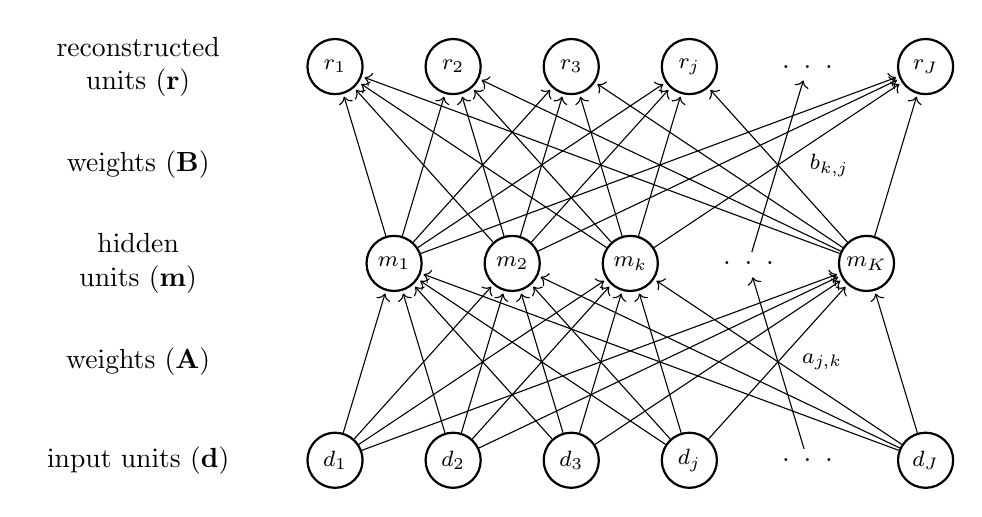
\begin{tikzpicture}[shorten >=1pt,->,draw=black!100]
	\def \rowtwoht{5cm}
	\def \weightstwo{3.75cm}
	\def \rowoneht{2.5cm}
	\def \weightsone{1.25cm}
	\def \basement{0cm}
	\tikzstyle{m-node}=[circle,draw=black!100,thick,inner sep=0pt,minimum size=7mm]
	\tikzstyle{r-node}=[circle,draw=black!100,thick,inner sep=0pt,minimum size=7mm]
	\tikzstyle{d-node}=[circle,draw=black!100,thick,inner sep=0pt,minimum size=7mm]
	\tikzstyle{dots}=[text width=5ex, text centered]
	\tikzstyle{annot}=[text width=17ex, text centered]
	% labels
	\node[annot] (r-layer) at (0cm,\rowtwoht) {reconstructed units ($\mathbf{r}$)};
	\node[annot] (weights) at (0cm,\weightstwo) {weights ($\mathbf{B}$)};
	\node[annot] (hidden-layer) at (0cm,\rowoneht) {hidden units ($\mathbf{m}$)};
	\node[annot] (weights) at (0cm,\weightsone) {weights ($\mathbf{A}$)};
	\node[annot] (d-layer) at (0cm,\basement) {input units ($\mathbf{d}$)};
	
	\node[dots] 	(m3)	at (7.75cm,\rowoneht)	 	{. . .};
	\node[dots] 	(r4) 	at (8.5cm,\rowtwoht)   		{. . .};
	\node[dots] 	(d4) 	at (8.5cm,\basement)   		{. . .};
	
	\footnotesize
	% hidden layer
	\node[m-node] 	(m0)	at (3.25cm,\rowoneht)		{$m_1$};
	\node[m-node] 	(m1)	at (4.75cm,\rowoneht)		{$m_2$};
	\node[m-node] 	(m2)	at (6.25cm,\rowoneht)	 	{$m_k$};
	\node[m-node] 	(m4)	at (9.25cm,\rowoneht)	 	{$m_K$};
	
	% reconstructed vector
	\node[r-node] 	(r0)	at (2.5cm,\rowtwoht)		{$r_1$};
	\node[r-node] 	(r1)	at (4cm,\rowtwoht)		{$r_2$};
	\node[r-node] 	(r2)	at (5.5cm,\rowtwoht)	 	{$r_3$};
	\node[r-node] 	(r3)	at (7cm,\rowtwoht) 		{$r_j$};
	\node[r-node] 	(r5) 	at (10cm,\rowtwoht)   		{$r_J$};
	%\node[r-node] 	(r6) 	at (9.75cm,\rowoneht)   	{$r_J$};
	
	% data vector
	\node[d-node] 	(d0)	at (2.5cm,\basement)		{$d_1$};
	\node[d-node] 	(d1)	at (4cm,\basement)		{$d_2$};
	\node[d-node] 	(d2)	at (5.5cm,\basement)	 	{$d_3$};
	\node[d-node] 	(d3)	at (7cm,\basement) 		{$d_j$};
	\node[d-node] 	(d5) 	at (10cm,\basement)   		{$d_J$};
	%\node[d-node] 	(d6) 	at (9.75cm,\basement)   	{$d_J$};
	
	\path
		(d0)	edge	node	{}	(m0)
		(d0)	edge	node	{}	(m1)
		(d0)	edge	node	{}	(m2)
		%(d0)	edge	node	{}	(m3)
		(d0)	edge	node	{}	(m4)
		%	
		(d1)	edge	node	{}	(m0)
		(d1)	edge	node	{}	(m1)
		(d1)	edge	node	{}	(m2)
		%(d1)	edge	node	{}	(m3)
		(d1)	edge	node	{}	(m4)
		%
		(d2)	edge	node	{}	(m0)
		(d2)	edge	node	{}	(m1)
		(d2)	edge	node	{}	(m2)
		(d2)	edge	node	{}	(m4)
		%
		(d3)	edge	node	{}	(m0)
		(d3)	edge	node	{}	(m1)
		(d3)	edge	node	{}	(m2)
		(d3)	edge	node	{}	(m4)
		%
		(d4)	edge	node[right=2mm]	{$a_{j,k}$}	(m3)
		%
		(d5)	edge	node	{}	(m0)
		(d5)	edge	node	{}	(m1)
		(d5)	edge	node	{}	(m2)
		(d5)	edge	node	{}	(m4)
	 
		(m0)	edge	node	{}	(r0)
		(m0)	edge	node	{}	(r1)
		(m0)	edge	node	{}	(r2)
		(m0)	edge	node	{}	(r3)
		(m0)	edge	node	{}	(r5)

		(m1)	edge	node	{}	(r0)
		(m1)	edge	node	{}	(r1)
		(m1)	edge	node	{}	(r2)
		(m1)	edge	node	{}	(r3)
		(m1)	edge	node	{}	(r5)

		(m2)	edge	node	{}	(r0)
		(m2)	edge	node	{}	(r1)
		(m2)	edge	node	{}	(r2)
		(m2)	edge	node	{}	(r3)
		(m2)	edge	node	{}	(r5)

		(m3)	edge	node[right=3mm]	{$b_{k,j}$}	(r4)	
		
		(m4)	edge	node	{}	(r0)
		(m4)	edge	node	{}	(r1)
		(m4)	edge	node	{}	(r2)
		(m4)	edge	node	{}	(r3)
		(m4)	edge	node	{}	(r5);
		
\end{tikzpicture}
\end{center}
\caption{The ``classical'' autoencoder, one member of the general autoencoder family}
%: an input layer ($\mathbf{d}$), a hidden layer ($\mathbf{m}$), and an output layer
\label{fig:autoencoder}
\end{figure}

% First, there is a generic autoencoder concept
% The generic autoencoder concept has several subtypes.

%Both hidden nodes and surface nodes have activity values, i.e., values in $[0,1]$ that
%indicate whether a node is \textsc{on} (active) or \textsc{off} (inactive). Each surface-node activity 
%is a function of the hidden-node activities and the weights that connect the hidden nodes to the surface node in question.

%Each surface node is either \textsc{on} (active) or \textsc{off} (inactive) depending 
%on the hidden-node activities and
%the weights connecting hidden nodes to surface nodes. 

%\subsection{Architecture}
%\label{subsec:architecture}

%An MCMM can be viewed as a variant of the classical autoencoder
%network \citep{dayan-and-zemel:95}, a type of neural network used for
%unsupervised learning.  In autoencoders, a hidden layer is forced to
%learn a compression scheme, i.e., a lower-dimensional encoding, for
%a dataset.
 
%MCMMs are called \emph{Multiple Cause} Mixture Models because more
%than one hidden unit can take part in the activation of a surface
%unit.  
%This is illustrated in figure \ref{fig:mcmm}, where the nodes
%$\mathbf{m}$ are the hidden units, and $\mathbf{r}$ is the (reconstructed) surface
%vector.
%Each arc $c_{j,k}$ represents the weight on the connection between
%$m_k$ and $r_j$.
%The activity of $r_j$ is determined by a mixing function 
%(section~\ref{sec:mixing-function}).



\begin{figure}[htb]
\begin{center}
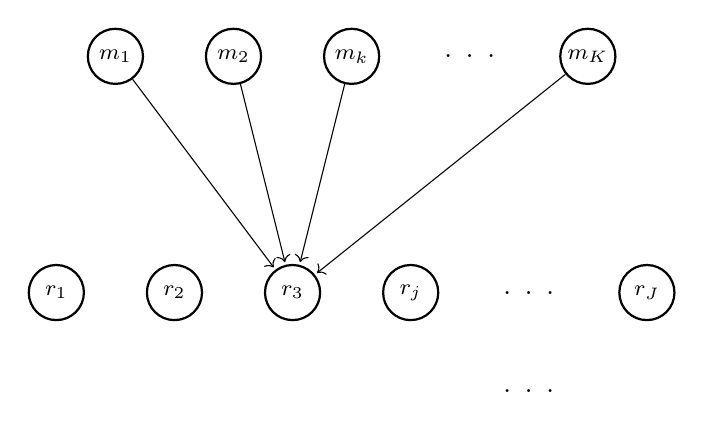
\begin{tikzpicture}[shorten >=1pt,->,draw=black!100]
	\def \rowtwoht{4.25cm}
	\def \weightlevel{2.75cm}
	\def \rowoneht{1.25cm}
	\def \basement{0cm}
	\tikzstyle{m-node}=[circle,draw=black!100,thick,inner sep=0pt,minimum size=7mm]
	\tikzstyle{r-node}=[circle,draw=black!100,thick,inner sep=0pt,minimum size=7mm]
	%\tikzstyle{d-node}=[circle,draw=black!100,fill=gray!45,thick,inner sep=0pt,minimum size=7mm]
	\tikzstyle{dots}=[text width=5ex, text centered]
	%\tikzstyle{annot}=[text width=17ex, text centered]
%	% labels
%	\node[annot] (hidden-layer) at (0cm,\rowtwoht) {hidden units ($\mathbf{m}$)};
%	\node[annot] (weights) at (0cm,\weightlevel) {weights ($\mathbf{C}$)};
%	\node[annot] (r-layer) at (0cm,\rowoneht) {predicted units ($\mathbf{r}$)};
	%\node[annot] (d-layer) at (0cm,\basement) {observed units ($\mathbf{d}$)};
	
	\node[dots] 	(m3)	at (7.75cm,\rowtwoht)	 	{. . .};
	\node[dots] 	(r4) 	at (8.5cm,\rowoneht)   		{. . .};
	\node[dots] 	(d4) 	at (8.5cm,\basement)   		{. . .};
	
	\footnotesize
	% hidden layer
	\node[m-node] 	(m0)	at (3.25cm,\rowtwoht)		{$m_1$};
	\node[m-node] 	(m1)	at (4.75cm,\rowtwoht)		{$m_2$};
	\node[m-node] 	(m2)	at (6.25cm,\rowtwoht)	 	{$m_k$};
	\node[m-node] 	(m4)	at (9.25cm,\rowtwoht)	 	{$m_K$};
	
	% reconstructed vector
	\node[r-node] 	(r0)	at (2.5cm,\rowoneht)		{$r_1$};
	\node[r-node] 	(r1)	at (4cm,\rowoneht)		{$r_2$};
	\node[r-node] 	(r2)	at (5.5cm,\rowoneht)	 	{$r_3$};
	\node[r-node] 	(r3)	at (7cm,\rowoneht) 		{$r_j$};
	\node[r-node] 	(r5) 	at (10cm,\rowoneht)   		{$r_J$};
	%\node[r-node] 	(r6) 	at (9.75cm,\rowoneht)   	{$r_J$};
	
	% data vector
%	\node[d-node] 	(d0)	at (2.5cm,\basement)		{$d_1$};
%	\node[d-node] 	(d1)	at (4cm,\basement)		{$d_2$};
%	\node[d-node] 	(d2)	at (5.5cm,\basement)	 	{$d_3$};
%	\node[d-node] 	(d3)	at (7cm,\basement) 		{$d_j$};
%	\node[d-node] 	(d5) 	at (10cm,\basement)   		{$d_J$};
	%\node[d-node] 	(d6) 	at (9.75cm,\basement)   	{$d_J$};
	
	\path 
		(m0)	edge	node	{}	(r2)
	
		(m1)	edge	node	{}	(r2)

		(m2)	edge	node	{}	(r2)
		%(m3)	edge	node {}	(r4)
		%(m3)	edge	node[right=1mm]	{$c_{j,k}$}	{}	(r0)
		%	
		(m4)	edge	node	{}	(r2);

		
\end{tikzpicture}
\end{center}
\caption{Architecture of a Multiple Cause Mixture Model (MCMM)} 
\label{fig:voting}
\end{figure}

%From source: "One  can  qualitatively  understand  the  difference  between  mixtures  and  products  by  observing  that  admixture distribution can have high probability for events when only a single expert assigns high probability to that event.  In contrast, a product can only have high probability for an events when all experts assign high probability to that event.  Hence, metaphorically speaking, a single expert in a mixture has the power to pass a bill while a single expert in a product has the power to veto it.Put another way, each component in a product represents a soft constraint, while each expert in a mixture represents a soft template or prototype. For an event to be likely under a product model, all constraints must1
%be (approximately) satisfied, while an event is likely under a mixture model if it (approximately) matches with  a  single  template."

%Bishop: "One approach is to apply gradient-based optimization techniques (Fletcher, 1987;Nocedal and Wright, 1999; Bishop and Nabney, 2008). Although gradient-based techniques are feasible, and indeed will play an important role when we discuss mixture density networks in Chapter 5, we now consider an alternative approach known as the EM algorithm which has broad applicability and which will lay the foundations for a discussion of variational inference techniques in Chapter 10." p. 435

%% Quora: "LDA is not a mixture model.  It is an admixture model or a mixed-membership model.
%Mixture models have a single latent variable that denotes which cluster they're in.  This is often written as an indicator variable z.  
%LDA is a model over documents (a bag of words), and has a latent variable for topic assignments for every token:  z1?zN
%Thus, words can belong to different clusters.  This intuitively makes sense because documents can be about more than one thing.  I.e., about both technology and business.  This often results in better models of real text than pure mixture models."

%The MCMM learns by comparing the reconstructed vector $\mathbf{r}_i$ 
%to its corresponding original datapoint $\mathbf{d}_i$. The discrepancy between
%the two is quantified by an \emph{objective function}. 
%If there is a discrepancy, the values of the nodes in
%$\mathbf{m}_i$ as well as the weights $\mathbf{C}$ are adjusted 
%in order to reduce the discrepancy as much as possible.
%See section~\ref{sec:mcmm-learning} for more on the learning process.

%Suppose data points $\mathbf{d}_u$ and $\mathbf{d}_v$ have some features in common.
%Then, as the MCMM tries to reconstruct them in $\mathbf{r}_u$ and $\mathbf{r}_v$, respectively,
%similarities will emerge between their respective hidden-layer vectors $\mathbf{m}_u$ and $\mathbf{m}_v$.
%In particular, the vectors $\mathbf{m}_u$ and
%$\mathbf{m}_v$ should come to share at least one active node, i.e., at least
%one $k \in K$ such that $m_{u,k} = 1$ and $m_{v,k} = 1$.
%This can serve as a basis for clustering;
%i.e., $m_{i,k}$ indicates whether $\mathbf{d}_i$ is a member of cluster $k$.
		
\section{Mixing Function}
\label{sec:mixing-function}

The mapping between the layer of hidden nodes $\mathbf{m}$ 
and the layer of surface nodes $\mathbf{r}$ is governed by a 
\emph{mixing function}, which is essentially
a kind of voting rule \citep{saund:94}. That is, maps from a set of (weighted)
input ``votes'' to a single output decision.  The output decision is 
an activity value for a particular surface-layer node. We will call the input votes
\emph{causes}. 

In its architecture, the \ac{MCMM} bears a striking resemblance to the 
Restricted Boltzmann Machine (RBM) \citep{smolensky:1986}. 
In particular, both the \ac{MCMM} and the \ac{RBM} are bipartite graphs. That is,
like an MCMM, an RBM has two layers of nodes with connections only between nodes of different layers, as described in chapter~\ref{ch:graph}). In addition, the RBM literature typically uses the terms \emph{hidden} and \emph{visible} to refer to these two layers, where \emph{visible} is analogous to (and essentially synonymous with) our term \emph{surface}. Moreover, learning in both MCMMs and RBMs is the result of an effort to reconstruct the actual data vectors in the surface (or visible) layer.

 one of the RBM layers is typical called the \emph{visible} layer,  hiddenas eter has a layer of hidden nodes and a layer of surface (or \emph{visible}) nodes. In the RBM literature, the surface layer is usually called the ``visible'' layer, but the two terms are synonymous. \footnote{In the RBM literature, authors typically the symbols $\textbf{h}$ and $\textbf{v}$ to refer to the hidden and visible (or surface) layers, respectively, whereas we are using $\textbf{m}$ and $\textbf{r}$, respectively, to refer the MCMM's hidden and surface layers.} 
%To make clear the correspondence between RBMs and MCMMs, let us apply the same set symbolfigure~\ref{fig:mcmm} to refer an RBM's components: 
%That is, in both, there are two layers of nodes---a hidden layer and a surface (or visible) layer, and there are no connections between nodes of the 
%same layer, as described in chapter~\ref{ch:graph}).
%Like an MCMM, an RBM is a bipartite graph. 
There are important differences, however. 

Both the \ac{MCMM} and the \ac{RBM} are bipartite graphs.
That is, both have two layers of nodes, with no connections between nodes of the 
same layer (as described in chapter~\ref{ch:graph}).  In a RBM, as in an \ac{MCMM}, 
one of these node layers functions as a hidden layer, and the other as the visible 
(or surface) layer \citep[see, e.g.,][]{mohamed-and-hinton:2010}. 
Consider \eqref{eq:rbm-prob-v} and \eqref{eq:rbm-prob-h}.
\begin{equation}\label{rbm:act-v}
r_j = \sigma\big(\sum_{k} c_{j,k} m_{k}\big)
\end{equation}
\begin{equation}\label{rbm:act-h}
m_k =\sigma\big(\sum_{j} c_{j,k} r_{j}\big)
\end{equation}
$p_i =\sigma(a_{i})$
where $\sigma(x)=frac{1}{1+\text{exp}(-x)}$ is the logistic function. 
\begin{align}
P(v|h) &= \prod_{i=1}^m P(v_i|h)  \label{eq:rbm-prob-v}\\
P(h|v) &= \prod_{j=1}^n P(h_j|v) \label{eq:rbm-prob-h}
\end{align}



%\begin{equation} \label{eq:rbm-prob-v}
%P(v|h) = \prod_{i=1}^m P(v_i|h)
%\end{equation}
%\begin{equation}  \label{eq:rbm-prob-h}
%P(h|v) &= \prod_{j=1}^n P(h_j|v)
%\end{equation}
 

********
One difference between 
the two, however, is that an RBM acts as a \emph{product} of experts, while an \ac{MCMM} 
acts as a kind of hybrid between a \emph{mixture of experts}, i.e., a (standard) mixture model, 
and a product of experts. To be clear, though, an \ac{MCMM} itself appears to be neither
 a sum nor a product of experts, not at least as these terms are usually construed. 


The ``experts" here 
%The RBM's equivalent of an MCMM's mixing function is a  \emph{product of experts}\citep{hinton:1999, hinton:2002}, where the ``experts" 
are the hidden units (along with their
respective weights). A product of experts is, as its name suggests, a multiplication, 
namely the product of all hidden-unit values, whereas a mixture of experts is a 
summation of these same values. In both MCMMs and RBMs, every expert casts 
a vote concerning whether a given surface node is to be \textsc{on} or \textsc{off} 
(i.e., 1 or 0). In an RBM, the votes are all multiplied together, so that if one vote is 0, 
the collective vote will be 0. In other words, in order for a given surface unit to be 1, 
\emph{every} hidden unit must vote 1.\footnote{If the values are continuous, i.e., in 
the interval $[0,1]$, every hidden unit must be very close to 1 in order for the surface 
unit to be close to 1.}

*******

In an MCMM, by contrast, every expert save one could cast a 0 vote, and the surface 
unit's value would still be nonzero. As long as \emph{at least} one of the hidden-unit 
votes is 1, the surface unit in question will be 1. On the other hand, if multiple experts 
vote 1, the surface unit's value is still 1. It will not exceed one even if all hidden units 
vote 1. Thus, the \ac{MCMM}'s method of combining expert votes behaves like a 
summation in some ways and product in others.  

Because an \ac{MCMM} is not a true mixture of experts, it cannot be a true mixture model. 
In a true mixture model, the expert votes must always sum to 1, and each surface unit's value 
is a \emph{weighted sum} of the votes from the hidden units. As the number of votes increases, 
the potency of each vote tends to decrease, unless most votes have weights that are close to zero. 
Mixture-of-experts models perform best when each surface unit's value is caused by a single 
expert, namely the best expert for that surface unit. Otherwise, the best expert's vote will be 
dampened. \marginpar{CITE?}

By contrast, in an \ac{MCMM}, a particular feature (i.e., surface unit) can be caused 
by one expert, all experts, or any number in between (where, again, the experts are hidden units).
An \ac{MCMM} is in this way similar to a \emph{mixed-membership} or \emph{admixture} model like 
Latent Dirichlet Allocation (LDA) \citep{blei-et-al:2003}. For example, 
when used in document clustering, LDA and other mixed-membership models
can (and generally do) assign a single document to multiple topics, which is to say a single document can be caused by multiple topics. If we replace \emph{document} and \emph{topics} with their equivalent terms in ULM, this statement becomes, `` 
A single \emph{word} can be caused by multiple \emph{morphs}.'' This is certainly true of Multimorph's MCMM, where words are represented as the feacture vectors $\textbf{r}_i$, and morphs are the hidden units, i.e., the components of the vectors $\textbf{m}_i$.
%In LDA, each document is associated with a distribution of topics, and each topic with a probabilistic distribution of words. Each is document is generated by randomly selecting a topic from the document's then randomly  A topic is randomly selected from the document's set of topicswherein
%the product of a process wherein the
Mixed-membership models can also attribute a single word to multiple topics, which is to say that a single word can be \emph{caused} by multiple topics. This statement's translation into morphological learning terms is,
%That is, a word, %e.g., %\emph{restaurant} 
%can be \emph{caused} by more than one topic.
%where each topic is a cluster of words. 
%In terms of morphological learning, the equivalent statement is, 
``A single \emph{word-internal feature (or character, etc.)} can be caused by more than one \emph{morph} at once,'' which is also true of Multimorph's MCMM (see section~\ref{sec:mixing-function} for more details).
Taken at face value, both of these statements (i.e., the ULM translations) are true of Multimorph's MCMM: the 
vectors $\textbf{r}_i$, which represent words, can certainly be caused by more than one morph (i.e., hidden unit), and moreover, an individual feature within $\textbf{r}_i$ can also be caused by more than one morph (see section~\ref{sec:mixing-function}). However, there is an importance difference here: 
 %and a word can be caused by more than one morph.'' 
 For the sake of clarity, table~\ref{tab:tm-to-ulm} gives topic-modeling terms alongside their equivalents in the unsupervised learning of morphology.
% Thus, a \emph{word} in topic-modeling is is equivalent to \emph{character}, a \emph{word-internal feature} in ULM (or perhaps \emph{character}, \emph{phoneme}, etc., depending on how words are represented in a given ULM approach).
\begin{table}{h}
\centering
\begin{tabular}{ccc}
Topic-Modeling & & ULM \\
document & $\to$ & word \\ %(i.e, feature-vector representing a word) \\
topic & $\to$ & morph/morpheme \\
word & $\to$ & word-internal feature or character \\
\end{tabular}
\caption{Some topic-modeling terms and their ULM equivalents. That is, for instance, \emph{documents}
in the context of topic modeling are equivalent to \emph{words} in the context of the unsupervised learning
of morphology.}
\label{tab:tm-to-ulm}
\end{table}
%in unsu\emph{words} in the case of topic modeling are analogous to
%to \emph{surface-level features} (or surface units) in the case of Multimorph and morphological learning. Likewise,
%\emph{topics} in topic modeling correspond to morphs in morphological learning, and 
However, according to \citet[][p. 4]{airoldi-et-al:2014}, ``[M]ixed membership models assume that individuals or observational units [i.e., words] may only partly belong to population mixture categories [i.e., topics] \dots. The degree of membership then is a vector of continuous, non-negative latent variables [i.e., hidden units] that add up to 1 (in mixture models, membership is a binary indicator).''
 Thus, an MCMM is not mixed-membership model, either, for in an MCMM, many individual latent variables (or hidden units) can be 1, which means that in an MCMM, a whole vector of hidden-unit activities can sum to a value greater than 1.

%\citep[e.g.,][]{miller-et-al:2016} 
%(and each cluster is represented as shared connections to a particular hidden unit). %The clusters would  \emph{food}, \emph{business}, and \emph{hospitality}, simultaneously.

Like latent Dirichlet allocation, MCMMs have
%also
been applied to document classification; \cite{sahami-et-al:96} 
use an \ac{MCMM} to group $I$ documents into $K$ clusters.  Documents are 
represented as vectors $\mathbf{x}_i$ of $J$ features. The features, i.e. surface units, 
each indicate the absence or presence of a particular word (cf. the $\mathbf{x}$ 
vector in figure~\ref{fig:mcmm}). The topics in \cite{sahami-et-al:96} are represented 
as the MCMM's hidden units $\mathbf{m}_i$. Documents are grouped into topic 
clusters by the learning process described below in section~\ref{sec:mcmm-learning}.
% are analogous to the morphological clusters in the present work; i.e., they each correspond to a hidden unit in $\mathbf{m}$. In particular, each hidden unit in$\mathbf{m}_i$ is the activity of a particular cluster for the $i$th datapoint--i.e., the $i$th document in the case of \cite{sahami-et-al:96}, and the $i$th word in the present work. 

%work hidden nodes in the vectors $  in the hidden-unit vectors $ were represented as $K$-length hidden-unit vectors $\mathbf{}$ document vector is thus analagous  wordsthe express purpose of mapping 
%particularly to map individual documents 
%each to multiple categories at once \cite{sahami-et-al:96}. %apply the \ac{MCMM} to 
By contrast, a true mixture model, such as \dots, is constrained to assigning each surface 
unit to a \emph{single} cause. In the case of 
document classification, this would mean each word (surface unit) could be attribute to no more than
one topic (or hidden unit). One might therefore describe any true
mixture model as a \emph{single-cause} mixture model. 

Each cause is a product of the form $m_{i,k} c_{j,k}$ for $k \in K$.
There are thus a total of $K$ distinct causes for a given surface node $r_{i,j}$. 
If the cause $m_{i,h} c_{j,h}$, where $h \in K$, is equal to $1$ or surpasses some
threshold, then $m_{i,h} c_{j,h}$ is an active cause.
%The input votes, are the activities of the hidden nodes,
%i.e., the $K$-length vector $\mathbf{m}_i$,
%coupled with their respective weights, i.e., the $K$-length vector 
%$\mathbf{c}_j$. 
%Any differentiable function
%that maps from the vector pair $(\mathbf{m}_i, \mathbf{c}_j)$ 
%to an activity value for $r_{i,j}$ can in theory serve as a mixing function. 
%There are thus an infinite number of theoretically possible mixing functions.

Following \cite{saund:94}, we use the Noisy-OR function \citep{pearl:1988}.
There are perhaps an infinite number of possible mixing functions. 
Any function that maps from a set of votes 
(and their respective weights) to a single output decision will suffice.
One possibility is the \textbf{Noisy-OR} function \citep{pearl:1988}:
 
\begin{equation}\label{eq:noisy-or}
r_{i,j} = 1 - \prod\limits_{k} (1 - m_{i,k} c_{j,k})
\end{equation}
% We will call the inputs to the Noisy-OR function \emph{causes}. Each cause is a product of the form $m_{i,k} c_{j,k}$. 
 The Noisy-OR function acts as a kind of \textit{OR} gate, or, to put it another way, 
 an``at-least-one" gate. That is, the surface node $r_{i,j}$ is $1$ as long as 
 \emph{at least one} cause is active.
 % (i.e., $m_{i,k} c_{j,k} = 1$ for at least one $k$ in $K$). 
 If two or more causes are active,
%$1$ (or $\ge$ than a threshold), 
$r_{i,j}$ is still going to be $1$. The output of Noisy-OR does not change 
as the number of active causes change, as long as there is at least one active cause.

Another possible mixing function is the \textbf{sigmoidal weighted sum}, 
the composition of the sigmoid function $S$ and the function $t_{i,j}$, 
which computes a weighted sum, i.e., the inner product of the cluster-activity 
vector $\mathbf{m}_i$ and the weight vector $\mathbf{c}_j$:

	\begin{align} %\label{eq:sigws}
	\label{eq:sig}
	r_{i,j} = S(t_{i,j}) &= \frac{1}{1 + e^{-t_{i,j}}} \quad %\\   %\qquad \text{where} \quad
	%\label{eq:ws}
	\text{where} \quad t_{i,j} = \sum_k m_{i,k} c_{j,k}
	\end{align}
This is the mixing (or activation) function that is typically used in classical autoencoders. 
Whereas the output of Noisy-OR is independent of the number of active 
causes (as long as there is at least one), the output of \eqref{eq:sig} does
change with the number of active causes: The value $t_{i,j} = \sum_k m_{i,k} c_{j,k}$ 
is clearly going to increase as the number of active clusters increases.
(i.e., products of the form $m_{i,k} c_{j,k}$ that equal $1$ or are greater than some threshold) 
As $t_{i,j}$ increases, $S(t_{i,j})$ will get closer to $1$; as %it
$t_{i,j}$ decreases, $S(t_{i,j})$ will get closer to $0$.

% What is the purpose of this section? To explain how an MCMM learns
% How should I present this information?
% Well, how does an MCMM learn?
%% The main idea is this: An MCMM learns by iteratively updating its parameters, the M and C matrices, so that
%% each update reduces the model's error.
%% What is the error? How is it measured?
%% How are the updates determined? 
%  OR THIS: An MCMM learns via numerical optimization. 
%% What is numerical optimization in general?
%% That is, what is a numerical optimization algorithm, and how does such an algorithm work (in general terms)?
%% What does Multimorph need in a numopt method? 
%% 
In choosing a numerical optimization method for Multimorph, we have to bear in mind two
facts about its MCMM: 
\begin{enumerate}
\item \textbf{It must be a \emph{bound constrained} method.} An MCMM's variables (i.e., the values 
in its M and C matrices)
%are bound by the values 0 and 1, 
%which is to say that the minimization of the MCMM's error function is 
have to stay
within the interval $[0,1]$, i.e., that they are \emph{bound} by 0 and 1.  \marginpar{Why?}. 
The problem of minimizing an MCMM's error function is thus a bound-constrained problem. 
That is, the problem is the subject to constraints, and these constraints take the form of 
lower and upper bounds (namely, 0 and 1) for each variable.
\item \textbf{It must be a \emph{nonlinear} optimization method.}
%  Multimorph's objective function is an error function, namely, the sum of squared error (SSE) (see equation \eqref{eq:sse}).  \emph{objective function}) is \emph{nonlinear}. 
Multimorph's objective function is a composition of functions, namely the composition of the sum-of-squared-error function \eqref{eq:sse} and the noisy-or mixing function \eqref{eq:noisy-or}, both of which are nonlinear; i.e., \emph{nonlinear} in the sense that their graphs are not straight lines. \footnote{Note that this sense of nonlinear is somewhat different from the sense employed in previous chapters, as in, e.g., the term \emph{nonlinear-nonsequential}.} We thus need an optimization technique that can handle nonlinear functions.
\end{enumerate} 

In short, Multimorph's learning process---the process of adjusting M and C in the direction of error reduction---is one of \emph{numerical optimization}. In particular, it employs the method proposed by
\citet{cheng-and-li:2012}, an \emph{active set} method conducive to \emph{bound-constrained} and \emph{nonlinear} problems. These are important attributes for our purposes because \dots.

\section{Learning}
\label{sec:mcmm-learning}
%\label{autoencoder-learning}
% A data compression scheme is useful only to the extent that it allows
% for the recovery of the source data from the compressed
% representations. In autoencoder terms, this means that 

\subsection{General Process}\label{sec:general}

The variables in an MCMM are the values in the $\mathbf{M}$ and $\mathbf{C}$ matrices. 
These values determine the 
reconstruction vectors in $\mathbf{R}$ via the Noisy-OR mixing function (\eqref{eq:noisy-or}). 
The MCMM's error is the discrepancy between  
$\mathbf{R}$ and the actual data $\mathbf{X}$. Learning occurs when the values in $\mathbf{M}$
and $\mathbf{C}$ are updated so as to to reduce this error. 
 
%reconstructions that are closer to the actual data (and thus a reduce 
%The reconstruction layer attempts to
%decode the hidden layer's representations and
In both the classical autoencoder and the MCMM, learning is the result of a search for an optimal valuation of the system's variables (or parameters), 
i.e., a valuation that minimizes 
%\emph{reconstruction error} $E$, 
the discrepancy between
reconstructed and original data points. That is, we want to find parameter 
values that minimize an error function. The search is conducted
via %some method of 
numerical optimization; 
we use a nonlinear conjugate gradient method.
Nonlinear conjugate gradient methods are a subcategory 
of numerical optimization methods, which are methods of 
optimizing an objective function $f$ by iteratively adjusting its parameters. 
Suppose the parameters to $f$ are the components of the vector $\mathbf{u} = [u_0,u_1, \dots, u_N]$.
 
If $f$ is an error function $E$ (as it is in our case), the optimization process is one of minimization, 
particularly one of finding the (global) minimum in $E(\mathbf{u}$), the curve of $E$ 
plotted against different valuations of $\mathbf{u}$.
The curve $E(\mathbf{u})$ is higher at some parameter valuations than others. 
%The optimization task is to find the parameter values that yield the minimal error (which is ideally zero). 
The basic approach to reduce the error by incrementally adjusting, or updating, the parameter vector $\mathbf{u}$. 

These updates are made component-wise over multiple iterations.
Each update is a ``step" with two distinct components, namely a step \emph{direction} $\mathbf{d}$ 
and a step \emph{size} 
%(or \emph{length} or \emph{magnitude}) 
$\alpha$, which is a scalar. The direction $\mathbf{d}$ is an array (or vector) 
of the same length as the parameter array $\mathbf{u}$, so that there is a 
dedicated direction component for each parameter component. 
The direction component of the update is supposed to ensure that error curve 
is descended rather than ascended. The step size $\alpha$ is meant to scale 
the update so that it is neither too small nor too large. That is, the update must 
be large enough to make a difference, but not so large that it overshoots the minimum. 
At iteration $t$, therefore, the parameter vector $\mathbf{u}$ is updated according 
to the following rule: 
\begin{equation}\label{eq:gen-update}
\mathbf{u}_{t+1} = \mathbf{u}_{t} + \alpha_t\mathbf{d}_{t}
\end{equation}

\begin{equation}\label{eq:mod-d-update}
\textbf{d}_{t} = -\textbf{g}_{t}  + \beta_{t} d_{t-1} - \theta_{t} \textbf{y}_{t-1}
\end{equation}
%(and thus each direction component vector is ``tailored'' to suit its corresponding parameter component). 

%tailoredparameter component is updated according to a tailored  vector the step must be such that the error curve is descended rather than ascended. The step must be sufficiently large that it makes a difference, but not so large that it overshoots the minimum. 
As for computing $\alpha_t$ and $\mathbf{d}_{t}$, there are various methods, and different combinations of these methods define different optimization algorithms. 


 for computing likely step directions and lengths. Conjugate gradient 
 methods incorporate a special scalar $\beta$ in computing the step direction. \citet{hager:2006} 
\citet{hager:2006}
In general, at iteration $t$, $\beta_{t+1}$ is updated, and the direction is then 


% as twwith two components, namely \emph{direction}  incremental adjustments 
% to the parameters so as to decrease the error, i.e., to descend the error curve by 
% manipulating the error function's parameters.  
 %falls in response to different paramenteone whose output rises and falls  param said to \emph{descend} the 

In general, different types of numerical optimization methods are distinguished 
by the way they choose the search direction.
Conjugate gradient (CG) methods come 
in both linear and nonlinear varieties. The former are designed to optimize 
linear objective functions; the latter are variants of linear methods, modified 
to handle nonlinear objective functions. 

%are variant of the latter distinct from linear conjugate gradient methods in that they are used to 

%The term \emph{optimization} in the context of numerical optimization can mean either minimization or maximization, depending on the nature of $f$. In our case, $f$ is an error function, and of course, error is something to be minimized. 

 iterative procedures that minimize an \emph{objective} function (also called an error function---by adjusting a set of variables. At each iteration $t$, the process adjusts each variable by adding a certain quantity to it. This quantity is computed differently in optimization methods. adjust by adding a cert comprises two factors: (1) a direction (i.e., positive or negative), and (2), a step length. consists of the following components:
\begin{enumerate}
\item $\mathbf{x}$: an array of variables $[x_0, x_1, ..., x_n, ..., x_N]$ to be updated
\item $f$: an objective function to be optimized (in our case, minimized).
\item $\nabla f$: the gradient of the objective function with respect to the variables $\mathbf{x}$.
\item $\beta$: a parameter used to compute the search direction $p$
\item $p$: the search direction
\item $\alpha$ Length of the step to taken along the search direction
\end{enumerate}

\subsection{Optimization}
%Compute \alpha_t and set xk+1  xk + \alpha_k p_k;
%Evaluate \nabla f_{k+1};
%\beta_{k+1}
%
%\nabla f^{T}
%k+1
%\nabla f_{k+1}
%\nabla f_{k}^{T} \nabla f_k
%
%p_{k+1}\leftarrow \nabla  f_{k+ 1 } + \beta_{k + 1} p_k 
%k \leftarrow k + 1

\cite{cheng-and-li:2012}
%gradient-based technique, e.g., gradient descent or
%the conjugate gradient method.
%


For the objective function, I used normalized \emph{``sum-of-squares'' error} (SSE), 
shown in equation \eqref{eq:sse}.
\begin{equation} \label{eq:sse}
E = \frac{1}{I \times J} \sum_{i} \sum_{j} {(r_{i,j} - d_{i,j})}^2
\end{equation}
 where $I \times J$ is the total number of features in the dataset.
The MCMM's task is to minimize this function by adjusting the
 values in $\mathbf{M}$ and $\mathbf{C}$, where
 %$I \times $ matrix $\mathbf{M}$ and the $J \times K$ matrix $\mathbf{C}$.
$\mathbf{M}$ is the $I \times K$ matrix that
% of dimensions $I \times K$,
encodes each data point's cluster-activity vector, 
and $\mathbf{C}$ is the $J \times K$ matrix that
%, of dimensions $J \times K$, 
encodes the weights between $\mathbf{m}_i$ and $\mathbf{r}_i$ for every $i \in I$ (see fig.~\ref{fig:example}). 
%$\mathbf{C}$ can also be interpreted as encoding the cluster centroids 
%(the clusters' ``average'' data points).
%Each column in $\mathbf{C}$ is in effect a feature vector; the $k^{\text{th}}$ column is 
%the $k^{\text{th}}$ cluster's average feature vector.
% \begin{align*}
% 	% E &= \frac{1}{I} \sum_{i} e_{i} \\
% 	% e_{i} &= \frac{1}{J} \sum_{j} {(r_{i,j} - d_{i,j})}^2
% 	E &= \frac{1}{I \times J} \sum_{i} \sum_{j} {(r_{i,j} - d_{i,j})}^2
% \end{align*}
% %\marginpar{Rationale for normalized SSE?} 
% which is minimized.
% rather than maximized. 
Active set methods classify indices. But to what end?
How is the concept \emph{stationary point} related to this question? 
 According to Wikipedia,
 ``A stationary point of a differentiable function of one variable is a 
 point on the graph of the function where the function's derivative is zero. 
 Informally, it is a point where the function stops increasing or decreasing 
 (hence the name).'' However, in a case of bound constrained optimization, 
 wherein each variable's value is constrained by a lower bound and an upper 
 bound, the derivative may \emph{not} be zero with respect to \emph{every} variable. 
 In such a case, therefore, a stationary point is more accurately defined as follows:
 \begin{equation}
  D_{it} =
    \begin{cases}
      1 & \text{if bank $i$ issues ABs at time $t$}\\
      2 & \text{if bank $i$ issues CBs at time $t$}\\
      0 & \text{otherwise}
    \end{cases}       
\end{equation}

What is a nonlinear conjugate gradient method?

\begin{equation}
p_k = -B_{k-1}\nabla f_k
\end{equation}

The \emph{size} (or \emph{length}) of each step was determined by the 
Armijo technique (CITE).  But maybe backtracking. Check.

%The basic idea is that we want 
%\begin{equation}
%\phi(\alpha)  f (x_k + \alpha p_k), \alpha >0
%\end{equation}
%; our techniques are described in section~\ref{subsec:objfunc}.
% There are a number of possibilities regarding the particular error
% function and gradient-based technique. We describe our choices in
% section~\ref{subsec:objfunc}.
% Any information loss in the compression will result in reconstructed
% vectors that differ from the original data points.  This is called
%the \emph{reconstruction error} is measured by some error function
%$err$, such as the
%%.  A typical error function is 
%the sum of squared error ($err_i = \sum_{j}{(d_{i,j} -
%  r_{i,j})}^2$). The global reconstruction error $E$, for the whole
%dataset, is the sum of all $err_i$.
%% over $i \in I$.
%%
%To discover a compression scheme with a minimal $E$, autoencoders
%use gradient-based search techniques, e.g., gradient descent or the
%conjugate gradient method.  We describe our error function in
%section~\ref{subsec:objfunc}.

% The autoencoder's goal is to discover a compression scheme that causes a minimal $E$, 
% and since $E$ is ultimately a function of $\mathbf{A}$ and $\mathbf{B}$, 
% this task reduces to finding the valuations for $\mathbf{A}$ and $\mathbf{B}$ that minimize $E(\mathbf{A},\mathbf{B}$). To this end, autoencoders use gradient-based search techniques, e.g., gradient descent or the conjugate gradient method. In the remainder of this section, we provide a very general description of an autoencoder's weight updating process. The details, especially the specific form of the weight-update function, depend on the particular gradient-based technique used. 

% Taking as input the data points $\mathbf{d}_i \in \mathbf{D}$, the network yields a reconstructed vector $\mathbf{r}_i$ for each individual $\mathbf{d}_i$. Because $\mathbf{D}$ contains $I$ data points, one epoch (i.e., one cycle through the dataset) is complete after $I$ iterations, whereupon ${E}(\mathbf{A}, \mathbf{B})$ is calculated, and each weight in $\mathbf{A}$ and $\mathbf{B}$ is adjusted in a way that furthers the descent of $E$ toward a minimum. 
% In particular, the algorithm adds to each 
% $b_{k,j} \in \mathbf{B}$ a quantity proportional to the negative gradient of 
% $E$ at $b_{k,j}$, or $-\frac{\partial E}{\partial b_{k,j}}$. 
% It similarly adds to each $a_{j,k} \in \mathbf{A}$
% a quantity proportional to the negative gradient of $E$ at $a_{j,k}$,
% or $-\frac{\partial E}{\partial a_{j,k}}$.
% These weight updates serve to improve the network's compression model, so that each successive epoch yields a smaller reconstruction error than the preceding epoch.
% The succession of epochs continues until $E$ falls below some small predesignated value.


% \subsection{The MCMM as an autoencoder variant}
% \label{subsec:mcmm-variant}

%\subsubsection{Architecture}
% Like the classical autoencoder, the MCMM has a hidden layer $\mathbf{m}$ and a reconstruction layer $\mathbf{r}$, as illustrated in figure \ref{fig:mcmm}. 
% However, the MCMM does not have an explicit
% data (or input) layer corresponding to the classical autoencoder's $\mathbf{d}$.
% Because the MCMM has only a two layers of nodes instead of three, it needs only a single layer of connecting weights, namely the weight matrix $\mathbf{C}$. This is a $J \times K$ matrix,
% since there are $K$ nodes in $\mathbf{m}$ and $J$ nodes in $\mathbf{r}$,
% and every $m_k$ must be linked to every $r_j$.

%\subsubsection{Mixing Function}
% MCMMs are distinguished by their propensity for learning hidden-unit activations and weight configurations that have clear interpretations.

% In the classical autoencoder, the activity $\phi(net)$ of any node $y$ is a
% function of its net raw input $net_y$, which is the weighted sum of $y$'s
% individual input signals (see \eqref{weighted-sum}). 
% The logistic sigmoid function $\phi$ then scales ${net}_y$ so that it falls within $[0,1]$.

% \begin{align*}
% r_{j} &= \sigma({net}_j) \\
% &= \sigma\big(\sum_k b_{k,j} \cdot m_k \big) \\
% &= \sigma \bigg(\sum_k b_{k,j} \cdot \sigma \big({net}_k \big) \bigg) \\
% &= \sigma \bigg(\sum_k b_{k,j} \cdot \sigma \big(\sum_j a_{j,k} \cdot d_j \big) \bigg) \\
% \end{align*}
% The activity of any given reconstruction node $r_j$ depends not only on the weights $\mathbf{B}$, but also on the weights $\mathbf{A}$.
% Moreover, $\mathbf{A}$ and $\mathbf{B}$ may differ.
% When $\mathbf{A} \ne \mathbf{B}$, the $\mathbf{B}$ weights can counteract the effects of the $\mathbf{A}$ weights, giving rise to unexpected activities among the $\mathbf{m}$ units and obscuring the  
% relationships between the $\mathbf{m}$ units and the $\mathbf{r}$ units.

% The MCMM, in contrast, is designed with the express purpose of providing a coherent causal explanation for regularities in surface data.
% What makes this possible?
% \begin{itemize} 
% \item \textit{Binary activities and weights.} Both the weights and the hidden unit activities are constrained to stay in $[0,1]$. At convergence, moreover, all values---both weights and hidden activities---should be either $0$ or $1$. \textit{Why is this important?} Binary values, i.e., \textsc{true} and \textsc{false}, have clear interpretations.
% \item \textit{Single layer of weights.} An MCMM has only one layer of weights. \textit{Why is this important?} The activities of the hidden units are manipulated directly in response to the reconstruction error.
% \item 
% \textit{How so?} In the classical autoencoder, the terms $m_kc_{j,k}, k \in K$ are combined linearly prior to sigmoid squashing. But MCMMs employ mixing functions such that the combination of these terms is nonlinear from the start. \textit{Why does this matter?} This ``total" nonlinearity encourages (?) weights to converge toward discrete values. The ultimate decision is then based on multiple discrete, either-or votes.
% \textit{Why, then, is clipping necessary?}
% \end{itemize}

% The classical autoencoder's activation function $\sigma({net}_y)$ is one possible mixing function,
% for it indeed takes the $K$ distinct input signals to node $y$ and yields a single activity value.
% However, as Saund points out, $\sigma({net}_y)$ is not well suited to the purpose of coherently distinguishing causes from non-causes. This is because $net_y$ is additive rather than multiplicative. Noisy-or is multiplicative:
% \begin{align*}
% r_{j} &= 1 - (1 - m_0c_{0,j}) \times (1 - m_1c_{1,j}) \times (1 - m_2c_{2,j}) \\
% &= 1 - (1 - 0) \times (1 - 0) \times (1 - 1) \\ 
% &= 1 - 1 \times 1 \times 0 \\
% &= 1
% \end{align*}
% As long as at least one $m_kc_{j,k} = 1$ (where $k = 0,1,\dots,K$), $r_{j}$ will be active,
% and $r_{j} = 0$ only if all products $m_kc_{j,k}$ are zero.
% Notice that $m_kc_{j,k} = 1$ only if both $m_k = 1$ and $c_{j,k} = 1$.
% On the other hand, with sigmoid squashing, $\sigma({net}_j)$ is never truly zero; it just gets infinitely close to zero.
% And $\sigma({net}_j)$ will be close to $1$ as long as ${net}_j = \sum_K m_k c_{j,k}$ is sufficiently large. 
% There are an infinite number of valuations for $\mathbf{m}$ and $\mathbf{c}_{j}$ that could give rise to a sufficiently large ${net}_j$.

% The function ${net}$ is an example of a linear mixing function. However, the autoencoder's mixing function
% is made nonlinear by $\phi({net}_y)$, which ``squashes" $net_y$ to fall within $[0,1]$.

%\subsubsection{Learning}
%\label{mcmm-learning}

%\paragraph{MCMM}

%\marginpar{MD: In fig.~\ref{fig:example}, we use $\mathbf{M}$, but
%  in previous figures we use $\mathbf{m}$.  Also, why is it sometimes
%  $\mathbf{m_k}$ and sometimes $\mathbf{m_{i,k}}$?  ($i$ refers to the
%  $i^{\text{th}}$ word?)}

The MCMM's learning process is similar to Expectation Maximization
(EM) in that at any given time it holds one set of variables 
fixed while optimizing the other set. We thus have two functions, \textsc{Optimize-M}
and \textsc{Optimize-C}, which take turns optimizing their respective matrices $\mathbf{M}$ 
\and $\mathbf{C}$:
While \textsc{Optimize-M} is optimizing $\mathbf{M}$, the weights $\mathbf{C}$ are treated as constants. Then, the cluster-membership vectors $\mathbf{m}_i$ in $\mathbf{M}$ is held fixed so that \textsc{Optimize-C} can optimize $\mathbf{C}$. The basic optimization algorithm within both \textsc{Optimize-M} and \textsc{Optimize-C} was 
The optimization algorithm itself was the
modified Polak--Ribi\'{e}re--Polyak method devised by \citet{cheng-and-li:2012}. This is method is conducive to the present case for two reasons: (1) While it is similar to the conjugate-gradient method, in particular, the version of the conjugate-gradient that employs the Polak--Ribi\'{e}re--Polyak update rule for $\beta$,  it is designed for non-linear optimization problems. 
\textit{non-linear bound-constrained} optimization.
for Large-Scale Nonlinear Bound Constrained
Optimization
Bound-constrained optimization. 
% However, if the algorithm is to optimize $\mathbf{M}$, it must first
% know $\mathbf{C}$, and vice versa.  Therefore, the algorithm can only
% focus on matrix at time, optimizing the one while holding the other
% fixed.
% The learning process consists of two distinct optimization
% functions:
%, \textsc{Optimize-M} and \textsc{Optimize-C}.
%\begin{description}
%\item[
% \textsc{Optimize-M} holds $\mathbf{C}$ fixed in order to optimize the
% cluster activity vectors in $\mathbf{M}$, while \textsc{Optimize-C}
% holds $\mathbf{M}$ fixed in order to optimize the cluster centroids in
% $\mathbf{C}$.
%\end{description}


The function \textsc{Optimize-M} loops over the $I$ cluster-activity vectors $\mathbf{m}_i$ in
$\mathbf{M}$, optimizing each one separately.  The optimization process itself is detailed in \cite{cheng-and-li:2012}.
%, one at a time.
%in $\mathbf{M}$, 
For each $\mathbf{m}_i$, \textsc{Optimize-M} enters an optimization 
loop over its $K$ components, adjusting each 
$m_{i,k}$ by a
quantity proportional to the negative gradient of $E$ at $m_{i,k}$. 
\marginpar{How is this proportion determined?} 
This loop repeats until $E$
ceases to decrease significantly,
whereupon \textsc{Optimize-M} proceeds to the next $\mathbf{m}_i$.  
The function \textsc{Optimize-C} consists of a single optimization loop over the 
entire matrix
$\mathbf{C}$. Each $c_{j,k}$ is adjusted by a quantity
proportional to the negative gradient of $E$ at $c_{j,k}$.
%, or $-\frac{\partial E}{\partial c_{j,k}}$.
%(in the case of gradient descent).  
%Since $E$ is simply
%$\sum_i e_i$, i.e., the sum of the errors of the individual data-point
%reconstructions, $-\frac{\partial E}{\partial c_{j,k}} = -\sum_i
%\frac{\partial e_i}{\partial c_{j,k}}$.  Thus, the adjustment to each
%$c_{j,k}$ takes into account the error of each reconstructed vector
%$\mathbf{r}_i$ in $\mathbf{R}$. However,
Unlike \textsc{Optimize-M}, which comprises $I$ separate optimization
loops, \textsc{Optimize-C} consists of just one, 
%optimizing the $\mathbf{C}$ matrix as a whole.  
When each of its $J \times K$
components has been adjusted, one round of updates to $\mathbf{C}$ is
complete.  $E$ is reassessed only between completed rounds of
updates. If the change in $E$ remains significant, another round begins.  
Both \textsc{Optimize-M} and \textsc{Optimize-C} are enclosed within 
an ``alternation loop" 
that alternates between the two functions, holding $\mathbf{C}$ fixed
during \textsc{Optimize-M}, and vice versa.
This alternation continues until $E$ cannot be decreased further. At
this point, an ``outer loop''
splits the cluster which contributes the most to the error, adds one
to the cluster count $K$, and restarts the alternation loop. The outer loop
repeats until it reaches an overall stopping criterion, e.g., $E = 0$.
%; otherwise, the function terminates.
 \subsection{Bound Constrained Optimization}
The optimization task is subject to the constraint %$0 le m_{i,k} ge 1$
that no value in $\mathbf{M}$ or $\mathbf{C}$ may exceed 1 or fall below 0. In other words,
it is a task of bound constrained optimization. Thus, whenever a value in either $\mathbf{M}$ or $\mathbf{C}$ is about
to fall below 0, it is set to 0. Likewise, whenever a value is about to exceed 1, it is set to 1
\citep{ni:yuan:1997}.
 %It repeatedly iterates over the $J \times K$ components of $\mathbf{C}$, stopping only when it finds a local minimum of $E$ is
  
%What is the inner loop and what is the outer loop?
%There are actually two inner loops: Opt-M is immediately followed by Opt-C. These two are encapsulated within a larger outer loop.
%What is the stopping criterion for the inner loop? What happens when this criterion is met?
%What is the stopping criterion for the outer loop?
%Cluster Splitting. Where does this enter the narrative?
%At this point, the algorithm then finds the worst cluster among the currently existing clusters and splits it, thereby increasing the cluster count $K$ by one.

\subsection{A Simple MCMM Example}
\label{subsec:example}

Fig.~\ref{fig:example} shows an example of an MCMM for two data points (i.e., $I = 2$).
The hidden cluster activities $\mathbf{M}$, the weights $\mathbf{C}$,
and the mixing function $r$ constitute a model that reproduces the
observed data points $\mathbf{D}$.
%
%\marginpar{MD: I don't quite understand the ``center vector''
  %statement}
%
The nodes $m_{i,k}$ represent cluster activities; if $m_{1,2} = 1$,
for instance, the second cluster is active for $\mathbf{d}_1$ (i.e.,
$\mathbf{d}_1$ is a member of cluster 2).
%
Note that the $J \times K$ weight matrix $\mathbf{C}$ is the same for
all data points, and
%
% For each data point, the arcs emanating from cluster
% 1 and cluster 2 represent the components of $\mathbf{C}$'s first and
% second rows, respectively. The $k$th row in $\mathbf{C}$ is thus
% uniquely associated with the $k$th cluster. Moreover, 
%
the $k^{\text{th}}$ row in $\mathbf{C}$ can be seen as the $k^{\text{th}}$
cluster's ``average" vector: the $j^{\text{th}}$ component in
$\mathbf{c}_k$ is 1 only if all data points in cluster $k$ have
1 at feature $j$.
%the $k^{\text{th}}$ row of $\mathbf{C}$ is in effect
%the center vector of the $k^{\text{th}}$ hidden cluster.
%
%In the figure, 

%\begin{figure}[htb!]
%\usetikzlibrary{positioning}
%%\begin{minipage}{.3\textwidth}
%\begin{center}
%%\subfigure[Learning in Progress]{
%\begin{tikzpicture}[shorten >=1pt,->,draw=black!100, scale=0.85]
%	\footnotesize
%%	\def \attic{5.95cm}
%%	\def \rowtwoht{5.4cm}
%%	\def \weightlevel{3.9cm}
%%	\def \rowoneht{2.4cm}
%%	\def \basement{1.8cm}
%%	\def \data{1cm}
%%	\def \china{0cm}
%
%	\def \attic{5.4cm}
%	\def \rowtwoht{4.8cm}
%	\def \weightlevel{3.6cm}
%	\def \rowoneht{2.4cm}
%	\def \basement{1.8cm}
%	\def \data{1cm}
%	\def \china{0cm}
%		
%	\tikzstyle{m-node}=[circle,draw=black!100,thick,inner sep=0pt,minimum size=6mm]
%	\tikzstyle{r-node}=[circle,draw=black!100,thick,inner sep=0pt,minimum size=6mm]
%	\tikzstyle{d-node}=[circle,draw=black!100,fill=gray!45,thick,inner sep=0pt,minimum size=6mm]
%	%\tikzstyle{dots}=[text width=5ex, text centered]
%	\tikzstyle{annot}=[text width=2.5em]
%	% labels
%	\tikzstyle{label}=[text width=2.5em, text centered]
%	\tikzstyle{formula}=[text width=30em, text centered]
%	
%	\scriptsize
%	\node[annot] (hidden-layer) at (0cm,\rowtwoht) {$\mathbf{M}_{(i,k)}$};
%	\node[annot] (weights) at (0cm,\weightlevel) {$\mathbf{C}_{(j,k)}$};
%	\node[annot] (r-layer) at (0cm,\rowoneht) {$\mathbf{R}_{(i,j)}$};
%	
%	% hidden layer
%	\scriptsize
%	\node[m-node] 	(ma00)	at (1.45cm,\rowtwoht)		{$.2$};
%	\node[m-node] 	(ma01)	at (3.35cm,\rowtwoht)		{$.9$};
%	\node[m-node] 	(ma10)	at (5.55cm,\rowtwoht) 	{$.8$};
%	\node[m-node] 	(ma11)	at (7.45cm,\rowtwoht)	 	{$.1$};
%	% \node[m-node] 	(m20)	at (9.65cm,\rowtwoht) 	{$.8$};
%	% \node[m-node] 	(m21)	at (11.55cm,\rowtwoht)	 	{$.9$};
%	
%	%\footnotesize
%	\node[label]	(ml00) 	at (1.45cm,\attic)		{$m_{1,1}$}; %1.75 -> 1.45
%	\node[label]	(ml01) 	at (3.35cm,\attic)		{$m_{1,2}$}; %3.05 -> 3.35
%	\node[label] 	(ml10)	at (5.55cm,\attic) 	{$m_{2,1}$};     %5.85 -> 5.55
%	\node[label] 	(ml11)	at (7.45cm,\attic)	 	{$m_{2,2}$}; %7.15 -> 7.45
%	% \node[label] 	(ml20)	at (9.65cm,\attic) 	{$m_{3,1}$};     %9.95 -> 9.65
%	% \node[label] 	(ml21)	at (11.55cm,\attic)	 	{$m_{3,2}$}; %11.25 -> 11.55
%	
%	\scriptsize
%	\node[r-node] 	(ra00)	at (1.1cm,\rowoneht)		{$.24$};
%	\node[r-node] 	(ra01)	at (2.4cm,\rowoneht)		{$.81$};
%	\node[r-node] 	(ra02)	at (3.7cm,\rowoneht)	 	{$.23$};
%	
%	\node[r-node] 	(ra10)	at (5.2cm,\rowoneht) 		{$.68$};
%	\node[r-node] 	(ra11) 	at (6.5cm,\rowoneht)   	{$.16$};
%	\node[r-node] 	(ra12)	at (7.8cm,\rowoneht)		{$.76$};
%	
%	% \node[r-node] 	(r20) 	at (9.3cm,\rowoneht)  		{$.71$};
%	% \node[r-node] 	(r21)	at (10.6cm,\rowoneht) 		{$.83$};
%	% \node[r-node] 	(r22) 	at (11.9cm,\rowoneht)   	{$.77$};
%	
%	\node[label] 	(rl00)	at (1.1cm,\basement)		{$r_{1,1}$};
%	\node[label] 	(rl01)	at (2.4cm,\basement)		{$r_{1,2}$};
%	\node[label] 	(rl02)	at (3.7cm,\basement)	 	{$r_{1,3}$};
%	
%	\node[label] 	(rl10)	at (5.2cm,\basement) 		{$r_{2,1}$};
%	\node[label] 	(rl11) 	at (6.5cm,\basement)   	{$r_{2,2}$};
%	\node[label] 	(rl12)	at (7.8cm,\basement)		{$r_{2,3}$};
%	
%%	\node[label] 	(rl20) 	at (9.3cm,\basement)  		{$r_{3,1}$};
%%	\node[label] 	(rl21)	at (10.6cm,\basement) 		{$r_{3,2}$};
%%	\node[label] 	(rl22) 	at (11.9cm,\basement)   	{$r_{3,3}$};
%
%	\draw[-] (4.45cm, \attic+1.5mm) -- (4.45cm, \basement-1.5mm);
%%	\draw[-] (8.55cm, \attic+1.5mm) -- (8.55cm, \basement-1.5mm);
%
%	\scriptsize
%	\path
%		(ma00)	edge	node [left]	{$.85$} (ra00)
%		(ma00)	edge	node [left,xshift=-1mm,yshift=3mm]	{$.1$}	(ra01)
%		(ma00)	edge	node [left,xshift=-1mm,yshift=8mm]	{$.95$}	(ra02)
%
%		(ma01)	edge	node [right,xshift=3mm,yshift=8mm]	{$.1$}	(ra00)
%		(ma01)	edge	node [right,xshift=1mm,yshift=3mm]	{$.9$}	(ra01)
%		(ma01)	edge	node [right]	{$.05$} (ra02)
%		%
%		(ma10)	edge	node [left] {$.85$} (ra10)
%		(ma10)	edge	node [left,xshift=-1mm,yshift=3mm]	{$.1$}	(ra11)
%		(ma10)	edge	node [left,xshift=-1mm,yshift=8mm] {$.95$}	(ra12)
%		
%		(ma11)	edge	node [right,xshift=3mm,yshift=8mm]	{$.1$}	(ra10)
%		(ma11)	edge	node [right,xshift=1mm,yshift=3mm]	{$.9$}	(ra11)
%		(ma11)	edge	node [right]	{$.05$} (ra12);
%		%
		% (m20)	edge	node [left]	{$.85$}	(r20)
		% (m20)	edge	node [left,xshift=-1mm,yshift=4mm]	{$.1$}	(r21)
		% (m20)	edge	node [left,xshift=-1mm,yshift=10mm]	{$.95$} (r22)
		
		% (m21)	edge	node [right,xshift=3mm,yshift=10mm]		{$.1$}	(r20)
		% (m21)	edge	node [right,xshift=1mm,yshift=4mm]{$.9$}	(r21)
		% (m21)	edge	node [right]	{$.05$}	(r22);		
		
%\end{tikzpicture}
%\label{fig:example:fig1}
%\caption{A simple MCMM example} % showing learning in progress}
%\label{fig:example:fig1}
%\end{center}
%\end{figure}

\begin{figure}[htb!]
\usetikzlibrary{positioning}
\begin{center}
\subfigure[Observed Data]{
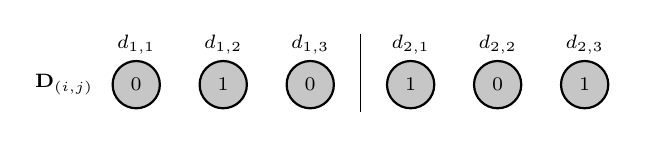
\begin{tikzpicture}[shorten >=1pt,->,draw=black!100, scale=0.85]
	\scriptsize
	\tikzstyle{label}=[text width=3em, text centered]
	\tikzstyle{annot}=[text width=2.5em]
	\tikzstyle{d-node}=[circle,draw=black!100,fill=gray!45,thick,inner sep=0pt,minimum size=6mm]
	
	\def \china{0.6cm}
	\def \data{0cm}
	
	\node[annot] (d-layer) at (0cm,\data) {$\mathbf{D}_{(i,j)}$};
	\draw[-] (4.45cm, \china+1.5mm) -- (4.45cm, \data-4.5mm);
%	\draw[-] (8.55cm, \china+1.5mm) -- (8.55cm, \data-4.5mm);
	%\draw[-] (-1cm, \china+.5cm) -- (13cm, \china+.5cm);
	%\draw[-] (-1cm, \data-.5cm) -- (13cm, \data-.5cm);
	
	\node[label] 	(dl00)	at (1.1cm,\china)		{$d_{1,1}$};
	\node[label] 	(dl01)	at (2.4cm,\china)		{$d_{1,2}$};
	\node[label] 	(dl02)	at (3.7cm,\china)	 	{$d_{1,3}$};
	
	\node[label] 	(dl10)	at (5.2cm,\china) 		{$d_{2,1}$};
	\node[label] 	(dl11) 	at (6.5cm,\china)   	{$d_{2,2}$};
	\node[label] 	(dl12)	at (7.8cm,\china)		{$d_{2,3}$};
	
	% \node[label] 	(dl20) 	at (9.3cm,\china)  		{$d_{3,1}$};
	% \node[label] 	(dl21)	at (10.6cm,\china) 		{$d_{3,2}$};
	% \node[label] 	(dl22) 	at (11.9cm,\china)   	{$d_{3,3}$};
	
	\node[d-node] 	(d00)	at (1.1cm,\data)		{$0$};
	\node[d-node] 	(d01)	at (2.4cm,\data)		{$1$};
	\node[d-node] 	(d02)	at (3.7cm,\data)		{$0$};

	\node[d-node] 	(d10)	at (5.2cm,\data)		{$1$};
	\node[d-node] 	(d11)	at (6.5cm,\data)		{$0$};
	\node[d-node] 	(d12)	at (7.8cm,\data)		{$1$};
	
	% \node[d-node] 	(d20)	at (9.3cm,\data)		{$1$};
	% \node[d-node] 	(d21)	at (10.6cm,\data)		{$1$};
	% \node[d-node] 	(d22)	at (11.9cm,\data)		{$1$};
\end{tikzpicture}
\label{fig:example:subfig0}
}
\end{center}

\usetikzlibrary{positioning}
%\begin{minipage}{.3\textwidth}
\begin{center}
\subfigure[Learning in Progress]{
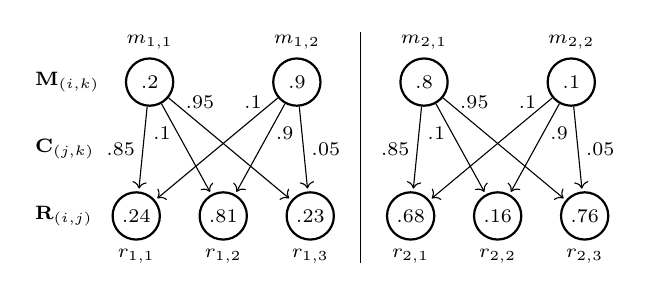
\begin{tikzpicture}[shorten >=1pt,->,draw=black!100, scale=0.85]
	\footnotesize
%	\def \attic{5.95cm}
%	\def \rowtwoht{5.4cm}
%	\def \weightlevel{3.9cm}
%	\def \rowoneht{2.4cm}
%	\def \basement{1.8cm}
%	\def \data{1cm}
%	\def \china{0cm}

	\def \attic{5cm}
	\def \rowtwoht{4.4cm}
	\def \weightlevel{3.4cm}
	\def \rowoneht{2.4cm}
	\def \basement{1.8cm}
	\def \data{1cm}
	\def \china{0cm}
		
	\tikzstyle{m-node}=[circle,draw=black!100,thick,inner sep=0pt,minimum size=6mm]
	\tikzstyle{r-node}=[circle,draw=black!100,thick,inner sep=0pt,minimum size=6mm]
	\tikzstyle{d-node}=[circle,draw=black!100,fill=gray!45,thick,inner sep=0pt,minimum size=6mm]
	%\tikzstyle{dots}=[text width=5ex, text centered]
	\tikzstyle{annot}=[text width=2.5em]
	% labels
	\tikzstyle{label}=[text width=2.5em, text centered]
	\tikzstyle{formula}=[text width=30em, text centered]
	
	\scriptsize
	\node[annot] (hidden-layer) at (0cm,\rowtwoht) {$\mathbf{M}_{(i,k)}$};
	\node[annot] (weights) at (0cm,\weightlevel) {$\mathbf{C}_{(j,k)}$};
	\node[annot] (r-layer) at (0cm,\rowoneht) {$\mathbf{R}_{(i,j)}$};
	
	% hidden layer
	\scriptsize
	\node[m-node] 	(ma00)	at (1.3cm,\rowtwoht)		{$.2$};
	\node[m-node] 	(ma01)	at (3.5cm,\rowtwoht)		{$.9$};
	\node[m-node] 	(ma10)	at (5.4cm,\rowtwoht) 	{$.8$};
	\node[m-node] 	(ma11)	at (7.6cm,\rowtwoht)	 	{$.1$};
	% \node[m-node] 	(m20)	at (9.65cm,\rowtwoht) 	{$.8$};
	% \node[m-node] 	(m21)	at (11.55cm,\rowtwoht)	 	{$.9$};
	
	%\footnotesize
	\node[label]	(ml00) 	at (1.3cm,\attic)		{$m_{1,1}$}; %1.75 -> 1.45
	\node[label]	(ml01) 	at (3.5cm,\attic)		{$m_{1,2}$}; %3.05 -> 3.35
	\node[label] 	(ml10)	at (5.4cm,\attic) 	{$m_{2,1}$};     %5.85 -> 5.55
	\node[label] 	(ml11)	at (7.6cm,\attic)	 	{$m_{2,2}$}; %7.15 -> 7.45
	% \node[label] 	(ml20)	at (9.65cm,\attic) 	{$m_{3,1}$};     %9.95 -> 9.65
	% \node[label] 	(ml21)	at (11.55cm,\attic)	 	{$m_{3,2}$}; %11.25 -> 11.55
	
	\scriptsize
	\node[r-node] 	(ra00)	at (1.1cm,\rowoneht)		{$.24$};
	\node[r-node] 	(ra01)	at (2.4cm,\rowoneht)		{$.81$};
	\node[r-node] 	(ra02)	at (3.7cm,\rowoneht)	 	{$.23$};
	
	\node[r-node] 	(ra10)	at (5.2cm,\rowoneht) 		{$.68$};
	\node[r-node] 	(ra11) 	at (6.5cm,\rowoneht)   	{$.16$};
	\node[r-node] 	(ra12)	at (7.8cm,\rowoneht)		{$.76$};
	
	\node[label] 	(rl00)	at (1.1cm,\basement)		{$r_{1,1}$};
	\node[label] 	(rl01)	at (2.4cm,\basement)		{$r_{1,2}$};
	\node[label] 	(rl02)	at (3.7cm,\basement)	 	{$r_{1,3}$};
	
	\node[label] 	(rl10)	at (5.2cm,\basement) 		{$r_{2,1}$};
	\node[label] 	(rl11) 	at (6.5cm,\basement)   	{$r_{2,2}$};
	\node[label] 	(rl12)	at (7.8cm,\basement)		{$r_{2,3}$};

	\draw[-] (4.45cm, \attic+1.5mm) -- (4.45cm, \basement-1.5mm);

	\scriptsize
	\path
		(ma00)	edge	node [left]	{$.85$} (ra00)
		(ma00)	edge	node [left,xshift=-1mm,yshift=2mm]	{$.1$}	(ra01)
		(ma00)	edge	node [left,xshift=-1mm,yshift=6mm]	{$.95$}	(ra02)

		(ma01)	edge	node [right,xshift=2.5mm,yshift=6mm]	{$.1$}	(ra00)
		(ma01)	edge	node [right,xshift=1mm,yshift=2mm]	{$.9$}	(ra01)
		(ma01)	edge	node [right]	{$.05$} (ra02)
		%
		(ma10)	edge	node [left] {$.85$} (ra10)
		(ma10)	edge	node [left,xshift=-1mm,yshift=2mm]	{$.1$}	(ra11)
		(ma10)	edge	node [left,xshift=-1mm,yshift=6mm] {$.95$}	(ra12)
		
		(ma11)	edge	node [right,xshift=2.5mm,yshift=6mm]	{$.1$}	(ra10)
		(ma11)	edge	node [right,xshift=1mm,yshift=2mm]	{$.9$}	(ra11)
		(ma11)	edge	node [right]	{$.05$} (ra12);
		%
		% (m20)	edge	node [left]	{$.85$}	(r20)
		% (m20)	edge	node [left,xshift=-1mm,yshift=4mm]	{$.1$}	(r21)
		% (m20)	edge	node [left,xshift=-1mm,yshift=10mm]	{$.95$} (r22)
		
		% (m21)	edge	node [right,xshift=3mm,yshift=10mm]		{$.1$}	(r20)
		% (m21)	edge	node [right,xshift=1mm,yshift=4mm]{$.9$}	(r21)
		% (m21)	edge	node [right]	{$.05$}	(r22);		
		
\end{tikzpicture}
\label{fig:example:subfig1}
}
\subfigure[Convergence]{

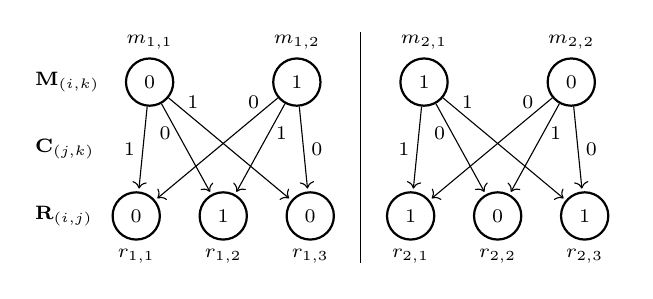
\begin{tikzpicture}[shorten >=1pt,->,draw=black!100, scale=0.85]
	\footnotesize
%	\def \attic{5.95cm}
%	\def \rowtwoht{5.4cm}
%	\def \weightlevel{3.9cm}
%	\def \rowoneht{2.4cm}
%	\def \basement{1.8cm}
%	\def \data{1cm}
%	\def \china{0cm}

%	\def \attic{5.2cm}
%	\def \rowtwoht{4.6cm}
%	\def \weightlevel{3.5cm}
%	\def \rowoneht{2.4cm}
%	\def \basement{1.8cm}
%	\def \data{1cm}
%	\def \china{0cm}

	\def \attic{5cm}
	\def \rowtwoht{4.4cm}
	\def \weightlevel{3.4cm}
	\def \rowoneht{2.4cm}
	\def \basement{1.8cm}
	\def \data{1cm}
	\def \china{0cm}
		
%	\def \attic{5.4cm}
%	\def \rowtwoht{5cm}
%	\def \weightlevel{3.9cm}
%	\def \rowoneht{2.4cm}
%	\def \basement{1.8cm}
%	\def \data{1cm}
%	\def \china{0cm}
	
	\scriptsize
	\tikzstyle{m-node}=[circle,draw=black!100,thick,inner sep=0pt,minimum size=6mm]
	\tikzstyle{r-node}=[circle,draw=black!100,thick,inner sep=0pt,minimum size=6mm]
	\tikzstyle{d-node}=[circle,draw=black!100,fill=gray!45,thick,inner sep=0pt,minimum size=6mm]
	\tikzstyle{annot}=[text width=2.5em]
	% labels
	\tikzstyle{label}=[text width=3em, text centered]
	\tikzstyle{formula}=[text width=30em, text centered]
	\node[annot] (hidden-layer) at (0cm,\rowtwoht) {$\mathbf{M}_{(i,k)}$};
	\node[annot] (weights) at (0cm,\weightlevel) {$\mathbf{C}_{(j,k)}$};
	\node[annot] (r-layer) at (0cm,\rowoneht) {$\mathbf{R}_{(i,j)}$};
	
	\node[m-node] 	(m00)	at (1.3cm,\rowtwoht)		{$0$};
	\node[m-node] 	(m01)	at (3.5cm,\rowtwoht)		{$1$};
	\node[m-node] 	(m10)	at (5.4cm,\rowtwoht) 	{$1$};
	\node[m-node] 	(m11)	at (7.6cm,\rowtwoht)	 	{$0$};
	% \node[m-node] 	(m20)	at (9.65cm,\rowtwoht) 	{$1$};
	% \node[m-node] 	(m21)	at (11.55cm,\rowtwoht)	 	{$1$};
	
	\node[label]	(ml00) 	at (1.3cm,\attic)		{$m_{1,1}$};
	\node[label]	(ml01) 	at (3.5cm,\attic)		{$m_{1,2}$};
	\node[label] 	(ml10)	at (5.4cm,\attic) 	{$m_{2,1}$};
	\node[label] 	(ml11)	at (7.6cm,\attic)	 	{$m_{2,2}$};
	% \node[label] 	(ml20)	at (9.65cm,\attic) 	{$m_{3,1}$};
	% \node[label] 	(ml21)	at (11.55cm,\attic)	 	{$m_{3,2}$};
	
	%\node[m-node] 	(m20)	[right of=m11,xshift=2cm]	 	{$1.0$};
	%\node[m-node] 	(m21)	[right of=m20,xshift=0.5cm]	 	{$1.0$};	
	% reconstructed vector
	\node[r-node] 	(r00)	at (1.1cm,\rowoneht)		{$0$};
	\node[label] 	(rl00)	at (1.1cm,\basement)		{$r_{1,1}$};
	\node[r-node] 	(r01)	at (2.4cm,\rowoneht)		{$1$};
	\node[label] 	(rl01)	at (2.4cm,\basement)		{$r_{1,2}$};
	\node[r-node] 	(r02)	at (3.7cm,\rowoneht)	 	{$0$};
	\node[label] 	(rl02)	at (3.7cm,\basement)	 	{$r_{1,3}$};
	
	\node[r-node] 	(r10)	at (5.2cm,\rowoneht) 		{$1$};
	\node[label] 	(rl10)	at (5.2cm,\basement) 		{$r_{2,1}$};
	\node[r-node] 	(r11) 	at (6.5cm,\rowoneht)   		{$0$};
	\node[label] 	(rl11) 	at (6.5cm,\basement)   		{$r_{2,2}$};
	\node[r-node] 	(r12)	at (7.8cm,\rowoneht)		{$1$};
	\node[label] 	(rl12)	at (7.8cm,\basement)		{$r_{2,3}$};
	
	% \node[r-node] 	(r20) 	at (9.3cm,\rowoneht)  		{$1$};
	% \node[label] 	(rl20) 	at (9.3cm,\basement)  		{$r_{3,1}$};
	% \node[r-node] 	(r21)	at (10.6cm,\rowoneht) 		{$1$};
	% \node[label] 	(rl21)	at (10.6cm,\basement) 		{$r_{3,2}$};
	% \node[r-node] 	(r22) 	at (11.9cm,\rowoneht)   		{$1$};
	% \node[label] 	(rl22) 	at (11.9cm,\basement)   		{$r_{3,3}$};
	
	\draw[-] (4.45cm, \attic+1.5mm) -- (4.45cm, \basement-1.5mm);
%	\draw[-] (8.55cm, \attic+1.5mm) -- (8.55cm, \basement-1.5mm);

	\path
		(m00)	edge	node [left] 	{$1$}	(r00)
		(m00)	edge	node [left,xshift=-1mm,yshift=2mm]	{$0$}	(r01)
		(m00)	edge	node [left,xshift=-3mm,yshift=6mm]	{$1$}	(r02)

		(m01)	edge	node [right,xshift=3mm,yshift=6mm]	{$0$}	(r00)
		(m01)	edge	node [right,xshift=1mm,yshift=2mm]	{$1$}	(r01)
		(m01)	edge	node [right]	{$0$}	(r02)
		%
		(m10)	edge	node [left] 	{$1$}	(r10)
		(m10)	edge	node [left,xshift=-1mm,yshift=2mm]	{$0$}	(r11)
		(m10)	edge	node [left,xshift=-3mm,yshift=6mm] {$1$}	(r12)
		
		(m11)	edge	node [right,xshift=3mm,yshift=6mm]	{$0$}	(r10)
		(m11)	edge	node [right,xshift=1mm,yshift=2mm]	{$1$}	(r11)
		(m11)	edge	node [right]	{$0$}	(r12);
		%
		% (m20)	edge	node [left]	{$1$}	(r20)
		% (m20)	edge	node [left,xshift=-1mm,yshift=4mm]	{$0$}	(r21)
		% (m20)	edge	node [left,xshift=-3mm,yshift=10mm]	{$1$} (r22)
		
		% (m21)	edge	node [right,xshift=3mm,yshift=10mm]		{$0$}	(r20)
		% (m21)	edge	node [right,xshift=1mm,yshift=4mm]{$1$}	(r21)
		% (m21)	edge	node [right]	{$0$}	(r22);		
\end{tikzpicture}
\label{fig:example:subfig2}
}

\begin{framed}
	\centering
	\small
	where
	$\begin{aligned}
	   r_{i,j} = 1 - \Pi_{k=1}^{K} (1 - m_{i,k}c_{j,k}) 
	\end{aligned}$
        \hspace{2em}
        [\textsc{noisy-or} function]
\end{framed}

\end{center}
\caption{A simple MCMM example} % showing learning in progress}
\label{fig:example}
\end{figure}

We can see that while learning is in progress, the cluster activities
($m_{i,k}$) and the cluster centers ($c_{j,k}$) are in flux, as the
error rate is being reduced, but that they converge to values of 0 and
1.  At convergence, a reconstruction node ($r_{i,j}$) is 1 if at least one
$m_{i,k}c_{j,k} = 1$ (and 0 otherwise).

%the activities and the centers are 1 and are 0 otherwise.

% \begin{figure*}[htb]
% \usetikzlibrary{positioning}
% \begin{center}
% \subfigure[Observed Data]{
% \begin{tikzpicture}[shorten >=1pt,->,draw=black!100]
% 	\scriptsize
% 	\tikzstyle{label}=[text width=3em, text centered]
% 	\tikzstyle{annot}=[text width=2.5em]
% 	\tikzstyle{d-node}=[circle,draw=black!100,fill=gray!45,thick,inner sep=0pt,minimum size=6mm]
	
% 	\def \china{0.6cm}
% 	\def \data{0cm}
	
% 	\node[annot] (d-layer) at (0cm,\data) {$\mathbf{D}_{(i,j)}$};
% 	\draw[-] (4.45cm, \china+1.5mm) -- (4.45cm, \data-4.5mm);
% 	\draw[-] (8.55cm, \china+1.5mm) -- (8.55cm, \data-4.5mm);
% 	%\draw[-] (-1cm, \china+.5cm) -- (13cm, \china+.5cm);
% 	%\draw[-] (-1cm, \data-.5cm) -- (13cm, \data-.5cm);
	
% 	\node[label] 	(dl00)	at (1.1cm,\china)		{$d_{1,1}$};
% 	\node[label] 	(dl01)	at (2.4cm,\china)		{$d_{1,2}$};
% 	\node[label] 	(dl02)	at (3.7cm,\china)	 	{$d_{1,3}$};
	
% 	\node[label] 	(dl10)	at (5.2cm,\china) 		{$d_{2,1}$};
% 	\node[label] 	(dl11) 	at (6.5cm,\china)   	{$d_{2,2}$};
% 	\node[label] 	(dl12)	at (7.8cm,\china)		{$d_{2,3}$};
	
% 	\node[label] 	(dl20) 	at (9.3cm,\china)  		{$d_{3,1}$};
% 	\node[label] 	(dl21)	at (10.6cm,\china) 		{$d_{3,2}$};
% 	\node[label] 	(dl22) 	at (11.9cm,\china)   	{$d_{3,3}$};
	
% 	\node[d-node] 	(d00)	at (1.1cm,\data)		{$0$};
% 	\node[d-node] 	(d01)	at (2.4cm,\data)		{$1$};
% 	\node[d-node] 	(d02)	at (3.7cm,\data)		{$0$};

% 	\node[d-node] 	(d10)	at (5.2cm,\data)		{$1$};
% 	\node[d-node] 	(d11)	at (6.5cm,\data)		{$0$};
% 	\node[d-node] 	(d12)	at (7.8cm,\data)		{$1$};
	
% 	\node[d-node] 	(d20)	at (9.3cm,\data)		{$1$};
% 	\node[d-node] 	(d21)	at (10.6cm,\data)		{$1$};
% 	\node[d-node] 	(d22)	at (11.9cm,\data)		{$1$};
% \end{tikzpicture}
% \label{fig:example:subfig0}
% }
% \end{center}

% \usetikzlibrary{positioning}
% %\begin{minipage}{.3\textwidth}
% \begin{center}
% \subfigure[Learning in Progress]{
% \begin{tikzpicture}[shorten >=1pt,->,draw=black!100]
% 	\footnotesize
% 	\def \attic{5.95cm}
% 	\def \rowtwoht{5.4cm}
% 	\def \weightlevel{3.9cm}
% 	\def \rowoneht{2.4cm}
% 	\def \basement{1.8cm}
% 	\def \data{1cm}
% 	\def \china{0cm}
	
% 	\tikzstyle{m-node}=[circle,draw=black!100,thick,inner sep=0pt,minimum size=6mm]
% 	\tikzstyle{r-node}=[circle,draw=black!100,thick,inner sep=0pt,minimum size=6mm]
% 	\tikzstyle{d-node}=[circle,draw=black!100,fill=gray!45,thick,inner sep=0pt,minimum size=6mm]
% 	%\tikzstyle{dots}=[text width=5ex, text centered]
% 	\tikzstyle{annot}=[text width=2.5em]
% 	% labels
% 	\tikzstyle{label}=[text width=3em, text centered]
% 	\tikzstyle{formula}=[text width=30em, text centered]
	
% 	\scriptsize
% 	\node[annot] (hidden-layer) at (0cm,\rowtwoht) {$\mathbf{M}_{(i,k)}$};
% 	\node[annot] (weights) at (0cm,\weightlevel) {$\mathbf{C}_{(j,k)}$};
% 	\node[annot] (r-layer) at (0cm,\rowoneht) {$\mathbf{R}_{(i,j)}$};
	
% 	% hidden layer
% 	\scriptsize
% 	\node[m-node] 	(m00)	at (1.45cm,\rowtwoht)		{$.2$};
% 	\node[m-node] 	(m01)	at (3.35cm,\rowtwoht)		{$.9$};
% 	\node[m-node] 	(m10)	at (5.55cm,\rowtwoht) 	{$.8$};
% 	\node[m-node] 	(m11)	at (7.45cm,\rowtwoht)	 	{$.1$};
% 	\node[m-node] 	(m20)	at (9.65cm,\rowtwoht) 	{$.8$};
% 	\node[m-node] 	(m21)	at (11.55cm,\rowtwoht)	 	{$.9$};
	
% 	%\footnotesize
% 	\node[label]	(ml00) 	at (1.45cm,\attic)		{$m_{1,1}$}; %1.75 -> 1.45
% 	\node[label]	(ml01) 	at (3.35cm,\attic)		{$m_{1,2}$}; %3.05 -> 3.35
% 	\node[label] 	(ml10)	at (5.55cm,\attic) 	{$m_{2,1}$};     %5.85 -> 5.55
% 	\node[label] 	(ml11)	at (7.45cm,\attic)	 	{$m_{2,2}$}; %7.15 -> 7.45
% 	\node[label] 	(ml20)	at (9.65cm,\attic) 	{$m_{3,1}$};     %9.95 -> 9.65
% 	\node[label] 	(ml21)	at (11.55cm,\attic)	 	{$m_{3,2}$}; %11.25 -> 11.55
	
% 	\scriptsize
% 	\node[r-node] 	(r00)	at (1.1cm,\rowoneht)		{$.24$};
% 	\node[r-node] 	(r01)	at (2.4cm,\rowoneht)		{$.81$};
% 	\node[r-node] 	(r02)	at (3.7cm,\rowoneht)	 	{$.23$};
	
% 	\node[r-node] 	(r10)	at (5.2cm,\rowoneht) 		{$.68$};
% 	\node[r-node] 	(r11) 	at (6.5cm,\rowoneht)   	{$.16$};
% 	\node[r-node] 	(r12)	at (7.8cm,\rowoneht)		{$.76$};
	
% 	\node[r-node] 	(r20) 	at (9.3cm,\rowoneht)  		{$.71$};
% 	\node[r-node] 	(r21)	at (10.6cm,\rowoneht) 		{$.83$};
% 	\node[r-node] 	(r22) 	at (11.9cm,\rowoneht)   	{$.77$};
	
% 	\node[label] 	(rl00)	at (1.1cm,\basement)		{$r_{1,1}$};
% 	\node[label] 	(rl01)	at (2.4cm,\basement)		{$r_{1,2}$};
% 	\node[label] 	(rl02)	at (3.7cm,\basement)	 	{$r_{1,3}$};
	
% 	\node[label] 	(rl10)	at (5.2cm,\basement) 		{$r_{2,1}$};
% 	\node[label] 	(rl11) 	at (6.5cm,\basement)   	{$r_{2,2}$};
% 	\node[label] 	(rl12)	at (7.8cm,\basement)		{$r_{2,3}$};
	
% 	\node[label] 	(rl20) 	at (9.3cm,\basement)  		{$r_{3,1}$};
% 	\node[label] 	(rl21)	at (10.6cm,\basement) 		{$r_{3,2}$};
% 	\node[label] 	(rl22) 	at (11.9cm,\basement)   	{$r_{3,3}$};

% 	\draw[-] (4.45cm, \attic+1.5mm) -- (4.45cm, \basement-1.5mm);
% 	\draw[-] (8.55cm, \attic+1.5mm) -- (8.55cm, \basement-1.5mm);

% 	\scriptsize
% 	\path
% 		(m00)	edge	node [left] 	{$.85$}	(r00)
% 		(m00)	edge	node [left,xshift=-1mm,yshift=4mm]	{$.1$}	(r01)
% 		(m00)	edge	node [left,xshift=-1mm,yshift=10mm]	{$.95$}	(r02)

% 		(m01)	edge	node [right,xshift=3mm,yshift=10mm]	{$.1$}	(r00)
% 		(m01)	edge	node [right,xshift=1mm,yshift=4mm]	{$.9$}	(r01)
% 		(m01)	edge	node [right]	{$.05$}	(r02)
% 		%
% 		(m10)	edge	node [left] 	{$.85$}	(r10)
% 		(m10)	edge	node [left,xshift=-1mm,yshift=4mm]	{$.1$}	(r11)
% 		(m10)	edge	node [left,xshift=-1mm,yshift=10mm] {$.95$}	(r12)
		
% 		(m11)	edge	node [right,xshift=3mm,yshift=10mm]	{$.1$}	(r10)
% 		(m11)	edge	node [right,xshift=1mm,yshift=4mm]	{$.9$}	(r11)
% 		(m11)	edge	node [right]	{$.05$}	(r12)
% 		%
% 		(m20)	edge	node [left]	{$.85$}	(r20)
% 		(m20)	edge	node [left,xshift=-1mm,yshift=4mm]	{$.1$}	(r21)
% 		(m20)	edge	node [left,xshift=-1mm,yshift=10mm]	{$.95$} (r22)
		
% 		(m21)	edge	node [right,xshift=3mm,yshift=10mm]		{$.1$}	(r20)
% 		(m21)	edge	node [right,xshift=1mm,yshift=4mm]{$.9$}	(r21)
% 		(m21)	edge	node [right]	{$.05$}	(r22);		
		
% \end{tikzpicture}
% \label{fig:example:subfig1}
% }
% \subfigure[Convergence]{

% \begin{tikzpicture}[shorten >=1pt,->,draw=black!100]
% 	\footnotesize
% 	\def \attic{5.95cm}
% 	\def \rowtwoht{5.4cm}
% 	\def \weightlevel{3.9cm}
% 	\def \rowoneht{2.4cm}
% 	\def \basement{1.8cm}
% 	\def \data{1cm}
% 	\def \china{0cm}
	
% 	\scriptsize
% 	\tikzstyle{m-node}=[circle,draw=black!100,thick,inner sep=0pt,minimum size=6mm]
% 	\tikzstyle{r-node}=[circle,draw=black!100,thick,inner sep=0pt,minimum size=6mm]
% 	\tikzstyle{d-node}=[circle,draw=black!100,fill=gray!45,thick,inner sep=0pt,minimum size=6mm]
% 	\tikzstyle{annot}=[text width=2.5em]
% 	% labels
% 	\tikzstyle{label}=[text width=3em, text centered]
% 	\tikzstyle{formula}=[text width=30em, text centered]
% 	\node[annot] (hidden-layer) at (0cm,\rowtwoht) {$\mathbf{M}_{(i,k)}$};
% 	\node[annot] (weights) at (0cm,\weightlevel) {$\mathbf{C}_{(j,k)}$};
% 	\node[annot] (r-layer) at (0cm,\rowoneht) {$\mathbf{R}_{(i,j)}$};
	
% 	\node[m-node] 	(m00)	at (1.45cm,\rowtwoht)		{$0$};
% 	\node[m-node] 	(m01)	at (3.35cm,\rowtwoht)		{$1$};
% 	\node[m-node] 	(m10)	at (5.55cm,\rowtwoht) 	{$1$};
% 	\node[m-node] 	(m11)	at (7.45cm,\rowtwoht)	 	{$0$};
% 	\node[m-node] 	(m20)	at (9.65cm,\rowtwoht) 	{$1$};
% 	\node[m-node] 	(m21)	at (11.55cm,\rowtwoht)	 	{$1$};
	
% 	\node[label]	(ml00) 	at (1.45cm,\attic)		{$m_{1,1}$};
% 	\node[label]	(ml01) 	at (3.35cm,\attic)		{$m_{1,2}$};
% 	\node[label] 	(ml10)	at (5.55cm,\attic) 	{$m_{2,1}$};
% 	\node[label] 	(ml11)	at (7.45cm,\attic)	 	{$m_{2,2}$};
% 	\node[label] 	(ml20)	at (9.65cm,\attic) 	{$m_{3,1}$};
% 	\node[label] 	(ml21)	at (11.55cm,\attic)	 	{$m_{3,2}$};
	
% 	%\node[m-node] 	(m20)	[right of=m11,xshift=2cm]	 	{$1.0$};
% 	%\node[m-node] 	(m21)	[right of=m20,xshift=0.5cm]	 	{$1.0$};	
% 	% reconstructed vector
% 	\node[r-node] 	(r00)	at (1.1cm,\rowoneht)		{$0$};
% 	\node[label] 	(rl00)	at (1.1cm,\basement)		{$r_{1,1}$};
% 	\node[r-node] 	(r01)	at (2.4cm,\rowoneht)		{$1$};
% 	\node[label] 	(rl01)	at (2.4cm,\basement)		{$r_{1,2}$};
% 	\node[r-node] 	(r02)	at (3.7cm,\rowoneht)	 	{$0$};
% 	\node[label] 	(rl02)	at (3.7cm,\basement)	 	{$r_{1,3}$};
	
% 	\node[r-node] 	(r10)	at (5.2cm,\rowoneht) 		{$1$};
% 	\node[label] 	(rl10)	at (5.2cm,\basement) 		{$r_{2,1}$};
% 	\node[r-node] 	(r11) 	at (6.5cm,\rowoneht)   		{$0$};
% 	\node[label] 	(rl11) 	at (6.5cm,\basement)   		{$r_{2,2}$};
% 	\node[r-node] 	(r12)	at (7.8cm,\rowoneht)		{$1$};
% 	\node[label] 	(rl12)	at (7.8cm,\basement)		{$r_{2,3}$};
	
% 	\node[r-node] 	(r20) 	at (9.3cm,\rowoneht)  		{$1$};
% 	\node[label] 	(rl20) 	at (9.3cm,\basement)  		{$r_{3,1}$};
% 	\node[r-node] 	(r21)	at (10.6cm,\rowoneht) 		{$1$};
% 	\node[label] 	(rl21)	at (10.6cm,\basement) 		{$r_{3,2}$};
% 	\node[r-node] 	(r22) 	at (11.9cm,\rowoneht)   		{$1$};
% 	\node[label] 	(rl22) 	at (11.9cm,\basement)   		{$r_{3,3}$};
	
% 	\draw[-] (4.45cm, \attic+1.5mm) -- (4.45cm, \basement-1.5mm);
% 	\draw[-] (8.55cm, \attic+1.5mm) -- (8.55cm, \basement-1.5mm);

% 	\path
% 		(m00)	edge	node [left] 	{$1$}	(r00)
% 		(m00)	edge	node [left,xshift=-1mm,yshift=4mm]	{$0$}	(r01)
% 		(m00)	edge	node [left,xshift=-3mm,yshift=10mm]	{$1$}	(r02)

% 		(m01)	edge	node [right,xshift=3mm,yshift=10mm]	{$0$}	(r00)
% 		(m01)	edge	node [right,xshift=1mm,yshift=4mm]	{$1$}	(r01)
% 		(m01)	edge	node [right]	{$0$}	(r02)
% 		%
% 		(m10)	edge	node [left] 	{$1$}	(r10)
% 		(m10)	edge	node [left,xshift=-1mm,yshift=4mm]	{$0$}	(r11)
% 		(m10)	edge	node [left,xshift=-3mm,yshift=10mm] {$1$}	(r12)
		
% 		(m11)	edge	node [right,xshift=3mm,yshift=10mm]	{$0$}	(r10)
% 		(m11)	edge	node [right,xshift=1mm,yshift=4mm]	{$1$}	(r11)
% 		(m11)	edge	node [right]	{$0$}	(r12)
% 		%
% 		(m20)	edge	node [left]	{$1$}	(r20)
% 		(m20)	edge	node [left,xshift=-1mm,yshift=4mm]	{$0$}	(r21)
% 		(m20)	edge	node [left,xshift=-3mm,yshift=10mm]	{$1$} (r22)
		
% 		(m21)	edge	node [right,xshift=3mm,yshift=10mm]		{$0$}	(r20)
% 		(m21)	edge	node [right,xshift=1mm,yshift=4mm]{$1$}	(r21)
% 		(m21)	edge	node [right]	{$0$}	(r22);		
% \end{tikzpicture}
% \label{fig:example:subfig2}
% }

% \begin{framed}
% 	\centering
% 	\small
% 	where
% 	$\begin{aligned}
% 	   r_{i,j} = 1 - \Pi_{k=1}^{K} (1 - m_{i,k}c_{j,k}) 
% 	\end{aligned}$
% \end{framed}

% \label{fig:example}
% \caption{MCMM example showing learning in progress}
% \end{center}
% \end{figure*}

 % The MCMM
\chapter{AUTONOMOUS MORPHOLOGY AS A TARGET OF LEARNING}
\label{autonomous}

%Or (Toward) Learning Morphology By Itself
%%%%%%%%%%%%%%%%%%%%%%%%%%%%%%%%
%% The main point of this chapter is the following: "It's not implausible to 
%% take a non-morpheme-based approach, to assume that morphology
%% is independent of phonology and syntax." Put another way, the main goal
%% is to justify taking a non-morpheme-based approach.
%%
%% This justification will mainly involve pointing out that many scholars
%% argue for autonomous morphology in one way or another. I will basically
%% be citing precedents. These the authors of the "Word-and-Paradigm" (WP) camp.
%% Aronoff is in this group, but he is not the only one. Who else? Whom shall describe
%% in some depth, and whom shall I merely mention in passing? In passing: Anderson,
%% Mathews, [Network morphology], ...
%% In some depth: Stump, Aronoff
%% However, most WP proponents these days, assume that Aronoff's morphomes exist.
%% and use the term morphome in their own theories.
%Where the \ac{ULM}  
%``Unsupervised Learning of Morphology" is concerned, what 
%is the learning target? The most immediate answer would 
%seem to be ``morphology,"
%
%but this answer would be ambiguous. You see...
%If one should ask a few linguists to summarize over the 
%meaning of \emph{morphology}
%of \emph{morphology}.
%One of the most pernicious 
%[and yet potentially most solvable] 
%problems in \ac{ULM} 
%%the Unsupervised Learning of 
%%Morphology (\ac{ULM} ) 
%is that its researchers do not seem to understand what
%their systems are learning. That is, morphological status
%what
%their systems
\section{Introduction}
Many morphologists in recent decades have rejected the notion of the morpheme---a concept that inextricably binds morphology to syntax and semantics---in favor of approaches that regard morphology as autonomous, i.e., as independent 
of both syntax/semantics and phonology. The principle objective of this chapter is to 
%\begin{itemize}
%\item 
show that autonomous morphological units are legitimate learning targets for a \ac{ULM}  system. In fact, as we shall soon, autonomous morphology is more than just legitimate; it is the only possible learning target for \ac{ULM}  as it is conventionally defined. %, i.e., to show that it makes sense to try to learn morphological units that are not morphemes.
%\item 
In the course of the discussion, we shall consider some of the more prominent theories of autonomous morphology, contrasting them with ``non-automonous" approaches, and  noting their significance to \ac{ULM} (and Multimorph in particular).

%and discuss their signifance where relationship to \ac{ULM}  and, more specifically, to Multimorph.
%\end{itemize}
% is to demonstrate that autonomous morphology is more than as a earning target for a \ac{ULM}  system. However, autonomous morphology, as we shall see, is more   in doing so, we shall  But more than that, this chapter will show , %an unsupervised morphological learning system, 
%instead to develop\emph{autonomous morphology} refers to a view of morphology wherein morphology is considered to be independent of both syntax/semantics and phonology.  often used to describe morphological theories 
%The main objective of this chapter is to demonstrate that not only is autonomous morphology


\section{The Unsupervised Learning of \textit{What}, Exactly?}
\label{sec:what-exactly}
In the \ac{ULM} literature, authors often use the word \emph{morpheme(s)} 
when describing their the systems' \emph{learning target(s)}, i.e., what their systems are meant to learn and 
output, as well as the features that compose their input feature vectors.
\cite{poon-et-al:2009}, for example, use two main categories 
of features, one of which they refer to as \emph{morpheme-context} features (see chapter \ref{ch:lit-review}).
\cite{goldsmith:2001, goldsmith:2006} also uses the word 
\emph{morpheme}.
%The word \emph{morpheme} is often present in the very titles of papers, e.g., 
%``Unsupervised Discovery of Morphemes" \citep{creutz-and-lagus:2002} and 
%``Unsupervised Models for Morpheme Segmentation and Morphology 
%Learning" \citep{creutz-and-lagus:2007}, 
%both titles by the creators of Morfessor \citep{creutz-and-lagus:2002, 
The creators of Morfessor 
\citep{creutz-and-lagus:2002, 
creutz-and-lagus:2005, creutz-and-lagus:2007}
%They also use \emph{morpheme} in the text of their papers, e.g.,
use a range of terms, including 
\emph{morpheme},
\emph{morpheme-like}, and \emph{morph}. The following quotations 
illustrate these usages (emphasis added):
\begin{exe}
\ex ``The model presented in this 
work provides a good means for the segmentation of words into 
\textbf{morphemes} \citep[][p. 6]{creutz-and-lagus:2007}. 
\ex``[W]e have demonstrated how the meaning and form of 
\textbf{morpheme-like} units can be modeled in a 
morphology induction task\dots" \citep{creutz-and-lagus:2005}.
\ex``The lexicon contains one entry for each distinct \textbf{morph} 
(morph type) in the 
segmented corpus" \citep[][p. 9]{creutz-and-lagus:2007}. 
\end{exe}
Creutz and Lagus seem to prefer the more general, theory-neutral term \emph{morph} 
in more formal or technical contexts. Indeed,
of the above three terms, they probably use 
\emph{morph} most frequently.

Moreover, \ac{ULM} researchers virtually never specify what they mean
when they use the word \emph{morphology}, even though there
are currently at least two fundamentally different schools of thought concerning the nature of morphology. These are the 
the \emph{morpheme-based} and \emph{lexeme-based} views, to borrow the labels that \cite{aronoff:1994} has assigned 
to these categories. The lexeme-based view, which has been gaining momentum in recent decades \citep{anderson:2017},
is that there exists an \emph{autonomous} layer of morphology, a layer that mediates between (morpho-)syntax
and phonological realization, but has neither meaning nor phonologically realized form in and of itself. Proponents
of lexeme-based morphology thus do not believe in pairings of form and meaning, i.e., \emph{morphemes}, as fundamental linguistic
units \cite{anderson:2015}. We shall further discuss the notion of autonomous morphology in section~\ref{autonomous}. 

One's morphological theory effects the way in which one interprets the output of a \ac{ULM}  system. 
If one describes a \ac{ULM}  system and its learning task in terms of 
morpheme-based morphology, one must also struggle to 
describe its output as consisting of morphemes, as do, for example, 
\cite{creutz-and-lagus:2007,creutz-and-lagus:2005}. In contrast, under a 
lexeme-based theory, one would view the output of a \ac{ULM}  system as 
consisting of \emph{autonomous} morphological units, i.e., 
expressly non-morpheme units. 
Thus, one's theory of morphology makes an implicit claim about the output of 
his/her \ac{ULM}  system.
%At this point, the attentive reader would be well-justified 
%in asking, 
%``WTF? What the F-word does Morfessor learn? What indeed 
%does \emph{any} 
%\ac{ULM}  system learn?" Indeed, dear reader, these are 
%excellent questions; 
%they will prove very significant to us, particularly the latter, 
%more general question, for it is directly relevant to what we 
%expect Multimorph is to learn.

The output of any machine learning system depends to 
a great extent on the nature of its input, which, in the case of the 
\emph{unsupervised} learning of morphology, 
depends on with the meaning of ``unsupervised to a large extent." 
%In the case of \ac{ULM} , the input is invariably a list of contextless words [cite?]. 
%And thus no syntactic or otherwise word-external features can be considered. 
%Any categories acquired by the algorithm thus cannot be conventional (or ``classical") 
%%morphemes, since morphemes are by definition minimal pairings of form and meaning.
%Now unsupervised learning is of course central to \ac{ULM} , 
%but one might might reasonably ask what ``unsupervised" 
%means in the context of morphological learning. 
All of the major \ac{ULM}  
systems take as input a list of independent tokenized words 
\citep[e.g.,][]{goldsmith:2001,baroni-et-al:2002,creutz-and-lagus:2005,poon-et-al:2009}
Thus, a convention seems to have emerged whereby, in the 
case of \ac{ULM} , the meaning of \emph{unsupervised} includes a
requirement that each word be free of morphosyntactic 
or semantic information. In practice,
this means being entirely free of context. I am 
not aware of a \ac{ULM} system that extracts features from the raw context surrounding a given word, i.e.,
the unanalyzed words adjacent to the unanalyzed word question. Presumably, this is because 
such a context would not be helpful to a machine learner. 
It would probably have to be abstracted and categorized 
(i.e., annotated) in order
for it to be helpful to a system. 
%The word underanalysis is help a system makes of the given unanalyzed 
%word in question.
%sequence of symbols, completely lacking in external information. 
%There is neither context nor annotation of any kind, and no thus 
%means of inducing semantics, i.e., of pairing forms with their 
%functions. 

Because morphemes are irreducible and arbitrary pairings of form and meaning
but in order to deduce meaning, one needs contextual information. Because
a \ac{ULM} system does not have access to context, it simply 
cannot learn classical morphemes. A \ac{ULM} system might learn 
subsequences of word strings that happen to resemble
 classical morphemes \emph{in form}, but only because there is always 
 morphological systems do tend to cooperate with syntax/semantics in some way, and in some 
 cases this cooperation appears more transparent and straightforward than
 in others.  However, this \ac{ULM} system would nevertheless be oblivious to what
 these pieces of form actually mean. Meaning is an essential component of the classical morpheme, and because
 meaning depends on context, there is no way to induce classical morphemes from contextless words.
%Since the words input to a \ac{ULM system are not accompanied by contextual features,
%there is no way to induce classical morphemes from contextless words, as meaning, which is determined by context, is 
%is an essential component of the classical morpheme.
%\footnote{Bloomfield, the leader of the American 
%Structuralists, provided the following early definition of the 
%\emph{morpheme}: ``[A] morpheme is a recurrent 
%(meaningful) form which cannot in 
%turn be analyzed into smaller recurrent (meaningful) forms. 
%Hence any unanalyzable word or formative is a morpheme" 
%\citep[][p. 155]{bloomfield:1926}.} 
Therefore, \ac{ULM} systems, particularly those which learn solely from 
from lists of raw, contextless words, simply cannot learn 
\emph{morphemes} in the strict sense of the term.

Consider, for example, Linguistica, the seminal 
\ac{ULM}  system developed by \cite{goldsmith:2001, goldsmith:2006}. 
Linguistica finds morphological relationships by filling in 
data structures 
called \emph{signatures} as it iterates over datasets comprising many
thousands of contextless words. Each signature $\sigma$ 
comprises 
two sets, $S$ and $A$, a set of stems and a set of affixes, 
respectively %, and is defined with respect to
%a corpus $C$. In particular, $\sigma= (S, A)$ if and only if
%\begin{itemize}
%   \item $S$ contains at least two stems, and $A$ at least two affixes.
%   \item Every stem in $S$ appears in $C$ with every affix in $A$. That is, every combination in $S \times A$ must be attested
%   in $C$, %That is, if $S = \{ s_1,s_2,s_3 \}$
%  % and $A = \{ a_1,a_2 \}$, then 
%   where $S \times A$ comprises $s_1 a_1$, $s_1 a_2$, $s_2 a_1$, $s_2 a_2$, $s_3 a_1$, and $s_3 a_2 $.
%\end{itemize}
A \emph{signature} is a pair of sets, namely a set of stems $S$ and 
a set of affixes $A$, such that each stem-affix combination in the cross 
product $S \times A$ is observed in the corpus. Additionally, $S$ and 
$A$ must each contain at least two members, with \textsc{null} being 
a permissible member, and each stem can belong to only one signature.  
%Crucially, each stem must occur in the corpus with each affix.  and likewise, each of the affixes must have been seen with each of the stems; 
%otherwise, the two sets do not constitute a signature.
%Given a tokenized corpus of words $W$, a \emph{signature} is a pairing of two sets, a set of stems $S$ and a set of affixes $A$, such that every stem-affix combination in $S \times A$ is attested in $W$; i.e., $S \times A \subseteq W$. Furthermore, $S$ and $A$ must each contain at least two members.
For example, a signature could be the following $S = \{ \text{act}, \text{back}, \text{mint} \}$ 
and $A = \{ \textsc{null}, \text{s}\}$. Every possible stem-affix combination is 
\begin{equation}
\label{eq:SxA}
S \times A = \{ \text{act}, \text{back}, \text{mint}, \text{act-s}, 
\text{back-s}, \text{mint-s}\}
\end{equation}
The fifth 
most common signature that Linguistica found among the words of 
\textit{Tom Sawyer} had as its affix set $\{\textsc{null}\textit{.ed.ing.s}\}$  \cite{goldsmith:2001}. 
%It corresponding stem set had 14 members. 
%\footnote{Its corresponding
%stem component had 14 members, but the identities of these stems are not given.}
%but
%the paper is the affix component in one of 
%the signatures that  Linguistica has extracted from the words of the novel \textit{Tom Sawyer}. 
The corresponding stem set had 14 members, though \cite{goldsmith:2001} 
does not identify the individual stems. 
In any case, the affix set \textsc{null}\textit{.ed.ing.s} represents 
a stem equivalence class. Its extraction would be an impressive achievement for any \ac{ULM}  system, and this
is but one of many such signatures that Linguistica has found. However, 
suppose we had no knowledge of \ac{EN}. It would then be impossible to deduce the nature 
of this equivalence class. We might
guess that it is a morphosyntactic category of \emph{some kind}, but since we would be ignorant
of the affixes' meanings/functions, this would be nothing more than a guess. 
%It would be entirely beyond our reach to attempt to guess the type of
%morphosyntactic category.
%We certainly could not begin to posit a particular morphosyntactic category.

An \ac{EN} speaker can probably deduce that \textsc{null}\textit{.ed.ing.s} are suffixes that attach to verbs,
but this it is the speaker's general competence in the language that informs this deduction, not anything in the 
signatures themselves. 
%[These stems were verbs clearly the nullsoft facts attached to the base case 
%the e d direct past tense the ing corresponds to the progressive or the present 
%participle in the s the third person singular present tense suffix.] 
%Now, it is not hard to guess the lexical category of the stems that accompany \textsc{null}\textit{.ed.ing.s}. 
%Clearly these are verbal suffixes.
%But it is not 
%But an \ac{EN} speaker would know this only because he/she know that \textsc{verb} + \textit{-ed} realizes a
%past-tense verb, \textsc{verb} + \textit{-s} realizes a 3rd-person 
%singular present-tense
%verb, and so on. 

Thus, although Linguistica does learn morphological equivalence classes, 
sets of stems that combine with the same affixes 
(and sets of affixes that combine with with the same stems) 
it does not learn to associate \textit{-s}, for example, 
with `3rd-person singular present-tense'. That is, it does not assign particular
meanings to the stems and affixes it discovers.
Nor would Linguistica know the particular meaning of any stem 
associated with a given affix set. 
Suppose that \{\textit{act}, \emph{jump}, and \emph{laugh}\} 
were the stem set associated with \textsc{null}\textit{.ed.ing.s}. 
Linguistica would thus have learned that these stems are the same 
in a way. But Linguistica would not have learned what this 
equivalence should have signified, not would have learned the semantic 
distinctions between the members of the same equivalence set. 
That is, even though \textit{act}, \emph{jump}, and \emph{laugh} 
share the same affix set, they do not share the same meaning. 
Thus, we must conclude that Linguistica does not learn morphemes 
in the classical sense, i.e., with each morpheme being a
pairing of one form and one meaning.

To be sure, this is not a failing on the 
part of Linguistica, which is indeed an effective 
unsupervised learner of morphology. Given the definition 
of the classical morpheme and the limited nature of 
Linguistica's input, it is simply not possible for 
Linguistica to learn true morphemes. First, because 
Linguistica is an \emph{unsupervised} learner, it has 
no access to the information it would need to assign 
%meanings to forms, as discussed above. Second, according to 
%many morphologists, morphemes do not adequately 
%account for the full range of morphological
%phenomena. Indeed, for these morphologists, morphemes do not exist.
Second, as we shall see in section~\ref{sec:morpho-theories}, morphemes do not adequately 
account for the full range of morphological phenomena \citep{anderson:2017}. 
For these reasons, morphemes are not reasonable 
targets of unsupervised morphological learning.
%do not even exist in the first place. 
 %the \emph{meaning} of \textit{act}, e.g., 
% that \emph{act} and
%\emph{jump} and \emph{laugh} do not share the same meaning, even though they (might) share
%the same affix set. Linguistica thus does not learn morphemes.
%We would then know each one means, include how it functions, i.e., how it interacts 
%(or does not interact with other morphemes). 
%For example, if know what \textit{act} and {-ed} mean individually, then we know, at 
%least according to the morpheme-based view of morphology, then we know what 
%and what \textit{act-ed} means, namely `act, \textsc{past-tense}'


%----------------------------------------
%Thus, Goldsmith?s signatures are clever devices for extracting meaning from raw, unannotated text. 
%\begin{enumerate}
%\item the nature of the algorithm 
%\item learns depends of course on the nature 
%\end{enumerate}
%of the algorithm, and there is wide variety of unsupervised learning algorithms out there.
%way in which these algorithms can be we (and on the nature of the input), 
%but in any case, the output of any \ac{ULM}  system will consist of forms entirely or almost entirely and be virtually void 
%of any real meaning. 
%It will find units that are building blocks of a sort, but these building blocks may not be what one expects. 
%They will serve to account for the internal structure of words while remaining utterly blind to the external contexts 
%might coincide the elements of word-internal structure. \citep{stump:2012}.

%\section{But if Not Morphemes, What?}
\section{A Spectrum of Morphological Theories}
\label{sec:morpho-theories}
%While Linguistica may learn morphology,  This is clearly apparent in 
%its signatures. % are clearly morphological structures.
%, I must say that it is an impressive system.
In the preceding section, we argued that Linguistica does not learn morphemes. The same can be said of Morfessor, 
the system of \cite{poon-et-al:2009}, and %virtually
%(if not absolutely) all 
every other \ac{ULM}  system. 
%but not morphemes, even though
% the word morpheme was used by Goldsmith.
 % the word morpheme. The Morfessor bunch at least seems to demonstrate some awareness that Morfessor 
%does not learning morphemes, using words like X and Y, yet even they use the word morpheme often enough.
 But how can we say that these systems learn morphology, but not morphemes? As it turns out,
 the existence of morphemes is by no means a sure thing.  
 %Many theories of morphology have been proposed over the last 1.2 million years. 
%are two opposing views in morphology. 
 %One believes in morphemes, the does not. 
 %However, these many theories, like so many tiny flakes of iron, have been drawn to one or the other of  two antithetical poles.
 %These camps have been described characterized in various ways.

\subsection{Stump's Taxonomy of Morphological Theories}
%%\subsubsection{Stump's Taxonomy of Morphological Theories}
\cite{stump:2001}'s oft-cited taxonomy of morphological theories 
consists of four categories. These four arise from two independent 
binary distinctions, namely \emph{lexical} vs. \emph{inferential} on the hand, and \emph{incremental} vs. \emph{realizational} on the other.
%In other words, anyone who is strongly considering formulating a new morphological theory has two overarching decisions to make, each corresponding to one of the binary distinctions. The first is whether the theory is 
%to be \emph{lexical} or \emph{inferential}. The second decision, which is orthogonal the first, is whether the theory is to be \emph{incremental} of \emph{realizational}.
%\begin{enumerate}
%   \item Decisition \emph{lexical} or \emph{inferential}? 
%   \item Is it \emph{incremental} or \emph{realizational}? 
%\end{enumerate}
%We might call the first decision the``\textsc{meaning source}" 
%decision and the second ``\textsc{direction}."  
%Consider for instance 
%the plural noun \textit{issues}. Suppose it is our morphologist's view that
%the meaning of \textit{issue+s} stems directly from the 
%meanings of the entries for \textit{issue} and \textit{-s} in the lexicon.
%She would then choose \emph{lexical} over \emph{inferential}. 
%But if she should instead believe that the meaning of 
%\textit{issue+s} is due to a rule like ``\textit{X+s} 
%is the plural form of \textit{X}," inferred from analogous forms like \textit{dog+s} and \textit{bike+s},
%she would then choose \textit{inferential} 
%instead of \emph{lexical}.
 
%As for the second decision, she would choose \emph{incremental} if she believes that 
%a word's meaning is built up as it acquires affixes; in others words, that the meaning of depends on its affixes
%  On the other hand, if she believed
%that a word's meaning determines its form and licenses a particular set
%of morphology exponents, she will
%choose \emph{realizational}. In 
\begin{exe}
\ex \textsc{First Distinction}: \textit{Lexical vs. Inferential} %(\citet{stump:2001}'s first distinction) \label{ex:d-one} 
\begin{xlist}
	\ex \textbf{Lexical}: The meaning of \textit{issue-s}, for example, is determined by the lexical entries of its components \textit{issue} and \textit{-s}.
%	  of the meanings of its components, which are specified in the lexicon. means what it does because its components, particularly /+s/, e mean what they do. as simply the composition of two lexical entries. 
%namely those for \textit{issue} and \textit{-s}. affixes, along with stems (for both are morphemes) have entries in the lexicon, and morphosyntactic properties are part of a morpheme's lexical entry. \label{ex:d-one-a}
	\ex \textbf{Inferential}: The meaning of \textit{issue-s} is determined by the meanings of related forms like \textit{dog-s} and \textit{bike-s},
%``treat morphological structure as grounded in the relations between classes of words" \citep[][p. 2]{anderson:2015shorthist}. %sim of form reflecting sim of content directly? The meaning of 
%In other words, %a form like
%\textit{issue+s} means what it does
%%, namely `\textit{issue} + \textsc{singular},'  
%because related forms like \textit{dog+s} and \textit{bike+s} mean what they do, 
with ``similarities of form [directly] reflecting similarities of content and vice versa" \citep[][p. 2]{anderson:2015shorthist}. \label{ex:d-one-b}
	\end{xlist}
\ex \textsc{Second Distinction}: \textit{Incremental vs. Realizational} %(\citet{stump:2001}'s second distinction) \label{ex:d-two} 
\begin{xlist} 
	\ex \textbf{Incremental}: Each affix has its own intrinsic meaning. 
	A form's \ac{MPS} is thus built up incrementally as it acquires affixes.
%	Thus, if an affix is removed from a word, the affix's meaning is also removed.  Conversely, whenever an affix is added to a form, the form's semantics ``annexes," as it were, the meaning of the affix (cf. the work of Ren\'e de Saussure). 
	\label{ex:d-two-a}
	\ex \textbf{Realizational}: A word's set of morphosyntactic properties 
	licenses a particular configuration of morphological exponents 
	(i.e., usually affixes of some sort). 
	%and thus realizes the phonological form. \label{ex:d-two-b}
	\end{xlist}
\end{exe}

%The two choices for the first decision are:
%\begin{description} 
%\item[Lexical:] The meaning of \textit{issue+s} is simply the composition of two lexical entries. 
%namely those for \textit{issue} and \textit{-s}. affixes, along with stems (for both are morphemes) have entries in the lexicon, and morphosyntactic properties are part of a morpheme's lexical entry.
%%She would then choose \emph{lexical} over \emph{inferential}.
%\item[Inferential theories] 
%``treats morphological structure as grounded in the relations between classes of words" \citep[][p. 2]{anderson:2015shorthist}. %sim of form reflecting sim of content directly? The meaning of 
%For example, the form 
%\textit{issue+s} means what it does, namely '\textit{issue} + \textsc{plural}'  because related forms like \textit{dog+s} and \textit{bike+s} mean what the they do, with ``similarities of form [directly] reflecting similarities of content and vice versa" (ibid.)
%%the rule ``\textit{X+s} 
%%is the plural form of \textit{X}," which is inferred from analogous forms like 
%%\textit{dog+s} and \textit{bike+s}.
%\end{description}
%The two choices for the second decision are:
%\begin{description}
%\item[Incremental:] Each affix has its own local meaning. Thus, if an affix is removed from a word, the innate meaning of the affix is also removed.  in the affix. Conversely, whenever an affix is added to a form, the form's semantics ``annexes," as it were, the meaning of the affix (cf. the work of Ren\'e de Saussure). 
%%final meaning depends on which affixes were added to it.
%\item[Realizational:] The meaning of a word, i.e., its set of morphosyntactic properties, determines its form. That is, the morphosyntactic properties invoke a rule that assembles the a particular group of morphological exponents.
%
%\emph{licenses} a particular set of exponents.
%\end{description}

By cross-combining the options of first distinction with those of the second, 
\cite{stump:2001} derives four categories of morphological theories. 
\emph{Lexical-Incremental} and \emph{Lexical-Realizational} theories 
on the one hand, and on the other, \emph{Inferential-Incremental} and 
\emph{Inferential-Realizational} theories. However, \citep{anderson:2017} 
notes that most theories fall into the \emph{Lexical-Incremental} and 
\emph{Inferential-Realizational} categories. Indeed, these are the two are 
the most extreme of the four categories in that they are entirely antithetical. 
The ongoing debate over the nature and status of morphology can largely 
be framed in terms of the opposition between these two categories. 

The distinction between \emph{Lexical-Incremental} 
and \emph{Lexical-Realizational} 
theories is essentially the same as the distinction 
that \cite{aronoff:1994} draws
between \emph{morpheme-based} and \emph{lexeme-based} 
views of morphology. Morpheme-based approaches regard 
the classical morpheme as the seat of meaning. %These are the legacy of Bloomfield and the descriptivists.
The concept of the morpheme and morpheme-centered morphological analysis
was developed by Bloomfield in the 1920s and 1930s 
\citep{bloomfield:1926, bloomfield:1933} and honed by his 
successors in the descriptivist program, e.g., % \cite[e.g.,][]{hocket:1947, harris:1955}.
\cite{hockett:1947} and \cite{harris:1955}.
It was \cite[][p. 161]{bloomfield:1933} who famously wrote, ``A linguistic form 
which bears no partial phonetic-semantic resemblance to any other form is a \emph{simple} form or \emph{morpheme}" (emphasis in the original). 
%\citep[][p. 161]{bloomfield:1933}.
%a distinct, irreducible pairing of form and meaning.  
That is, a morpheme, as a pairing of a form and a meaning, is a fundamental unit; it cannot be analyzed into smaller units
of form and meaning.
Moreover, Bloomfield and the descriptivists maintained that
each \emph{complex form}, i.e., each word comprising 
two or more morphemes, was \emph{exhaustively decomposable} 
into morphemes. That is, every phonological segment
in a given word had to be either a morpheme or part of a morpheme. 


%  ``Thus [A] morpheme is a recurrent (meaningful) form which cannot in turn be analyzed into smaller recurrent (meaningful) forms. Hence any unanalyzable word or formative is a morpheme" \cite[][p. 155]{bloomfield:1926}. It was Leonard Bloomfield, founder of descriptivism,  linguistic form which bears no partial phonetic-semantic resemblance to any other form is a \emph{simple} form or \emph{morpheme}." \citep[][p. 161]{bloomfield:1933}. Moreover, according to Bloomfield, every word comprises one or more morphemes, and every word must be \emph{exhaustively decomposable} into morphemes. That is, every phonological segment in a given word must either be a morpheme or part of morpheme. The concept of the morpheme and morpheme-centered morphological analysis
%was developed by Leonard Bloomfield \cite{bloomfield:1926, bloomfield:1933} and honed by his 
%descriptivist successors. 

The influence of Bloomfield and the descriptivists %(or American structuralists)
cannot be easily underestimated. Bloomfieldian concepts and methods 
pervade introductory linguistics courses and textbooks, both at
the undergraduate and graduate level. Any introductory text containing 
a unit on morphological analysis is going to present a methodology that 
is essentially Bloomfieldian \citep{anderson:2017}.
% morphological unit in an introductory linguistics textbook
%ccourse on morphology or general linguistics course teaches essentially 
%Bloomfieldian methods of morphological analysis. The morpheme is central concept in any undergraduate
%linguistics textbook. 
It is therefore perhaps no surprise that
computational linguists, including researchers in the field of \ac{ULM}, 
tend to presume %a morpheme-based morphology.
the reality of Bloomfieldian morphemes and the soundness of a 
Bloomfieldian view of morphology. The Bloomfieldian approach is essentially
the lexical-incremental approach.
%most familiar with and the type that all linguistics 
%undergraduates learn is the lexical-incremental type. 

By contrast, lexeme-based approaches (also called \emph{word-based} 
approaches) view the whole word as the seat of meaning. That is, the component 
parts of a complex word do not have their own predetermined meanings. 
Rather, 
there is a buffer layer between the level of phonological form and that of 
syntax/semantics. This
buffer consists of morphological rules that map from raw phonological 
strings to meanings.
\ac{PFM} \citep{stump:2001} 
posits a morphological architecture consisting of two kinds of paradigms: a \emph{content} paradigm and a \emph{form} paradigm.
% the level of the fully realized form. He also posits relations that map
%from one level to another. 
The cells of the former are related to those of the latter via
\emph{paradigm functions}.
% map from cells of the content paradigm (or \emph{content} cells) to cells of the form paradigm
A \ac{PF} takes the basic form of
\eqref{eq:PF}, where the lefthand side represents a particular cell in the 
content paradigm, and the righthand side a particular cell in the form paradigm. 
%The L represents a lexeme, and the X a stem. 
\begin{equation}
\label{eq:PF}
	\text{PF}\langle \text{L},\sigma \rangle = \langle \text{X}, \sigma^\prime \rangle
\end{equation}
The L represents a lexeme, and the X a stem,  i.e., the form correspondent of L. 
The \ac{MPS}s associated with content cell and form cell are $\sigma$ and 
$\sigma\prime$, respectively. In the canonical case, there is a one-to-one
correspondence between content cells and paradigm cells, and 
$\sigma = \sigma^\prime$.
Often, however, the mapping between content and form paradigm cells is 
not one-to-one, $\sigma \ne \sigma^\prime$, or both. A state of mismatch 
between $\sigma$ and 
$\sigma^\prime$ is called \emph{deponency}, it does not \emph{per se} 
throw off a one-to-one correspondence between content and form cells; 
that is, it does not change the number of form cells. Rather, deponency 
is a condition in which a content cell refers to one morphosyntactic property 
set $\sigma$, while its corresponding form cell refers to $\tau$, a different 
morphosyntactic property set. For example, a verb stem might take passive 
affixes in the active voice \citep{stewart-and-stump:2007}.

Another type of non-canonicity in content-to-form mappings is \emph{syncretism}. 
This type does cause a misalignment between the content and form cells, namely,
a many-to-one mapping, i.e., the form paradigm has fewer cells 
than the content paradigm. Consider, for example, table 
\ref{tab:engverbpres}, which shows both the content and form paradigms 
for the \ac{EN} lexeme \emph{kick} in the simple present tense.
The content paradigm has six cells, one for each combination of \textsc{person} 
and \textsc{number}, while the form paradigm has only two, one for the 
form that has no suffix (\textit{kick}) and the other for the form 
that ends in \textit{-s} (\textit{kicks}). 
 
%In other words, in cases of syncretism, the form paradigm has fewer cells 
%than the content paradigm.
\begin{table}[ht]
\centering % used for centering table
%\begin{tabular}{|*{3}{c|}} % centered columns (4 columns)
\begin{tabular}{c c c}
\hline\hline%inserts double horizontal lines
%& & \multicolumn{2}{c}{Syntactic Function} \\[-1ex] 
Content Paradigm & Form Paradigm & Realization \\ [0.5ex] % inserts table
\hline%heading
%$\langle$ \textsc{kick}, \textsc{p}:{1}, \textsc{n}:{sg} $\rangle$ & \multirow{5}{*}{$\langle$ \textsc{kick}, \{\textsc{p}:{1}$\vee${2}, \textsc{n}:{sg}$\vee${pl}\} $\rangle$} & \multirow{5}{*}{kick} \\ \cline{1-1}
$\langle \textsc{kick} \land \textsc{p:1}$, \textsc{n}:{sg} $\rangle$ & \multirow{5}{*}{$\langle \textsc{kick}, 
\{ ((\textsc{p:}\text{1}\vee\text{2}) \land (\textsc{n:}\text{sg} \vee \text{pl})) 
\vee (\textsc{p:}\text{3}\land \textsc{n:}\text{pl}) \} \rangle$} 
& \multirow{5}{*}{kick} \\ \cline{1-1}
$\langle \textsc{kick} \land \{\textsc{p:2}$, \textsc{n}:{sg}\} $\rangle$  &\\ \cline{1-1}
$\langle \textsc{kick} \land \{\textsc{p:1}$, \textsc{n}:{pl}\} $\rangle$  & \\ \cline{1-1}
$\langle \textsc{kick} \land \{\textsc{p:2}$, \textsc{n}:{pl}\} $\rangle$ &  \\ \cline{1-1}
$\langle \textsc{kick} \land \{\textsc{p:3}$, \textsc{n}:{pl}\} $\rangle$ & \\ \hline
$\langle \textsc{kick} \and \{\textbf{\textsc{p}:{3}}$, \textbf{\textsc{n}:{sg}}\} $\rangle$ & $\langle$ \textsc{kick}, \{\textbf{\textsc{p}:{3}}, \textbf{\textsc{n}:{sg}}\} $\rangle$  & kicks \\[0.5ex]
\hline %inserts single line
\end{tabular}
\label{tab:engverbpres} % is used to refer this table in the text
\caption{Dual-paradigm analysis of the \ac{EN} present tense} % title of Table
\end{table}

%\begin{equation}
%\label{eq:eng-verb-sync}
%	\{ \textsc{pers:3}\text{,} \, \textsc{num:}\text{sg,} \, \textsc{tns:}\text{pres} \} = \text{X}s
%\end{equation}
% (1 and (sg or pl)) or (2 and (sg or pl)) or (3 and pl)
%$(\text{1} \land (\text{sg} \vee \text{pl})) \vee (\text{2} \land (\text{sg} \vee \text{pl})) \vee (\text{3} \land \text{pl})$
%$\{ ((\text{\textsc{pers}:1}\vee\text{2}) \land (\textsc{num:}\text{sg} \vee \text{pl})) \vee (\textsc{pers:}\text{3} \land \textsc{num:}\text{pl}) \}$
%$\{ ((\text{\textsc{p}:1}\vee\text{2}) \land (\textsc{n:}\text{sg} \vee \text{pl})) \vee (\textsc{p:}\text{3} \land \textsc{n:}\text{pl}) \}$
Notice the unnaturalness of the two morphosyntactic classes in
the form-paradigm column in table \ref{tab:engverbpres}.
Classes like these abound in morphology.  
They are unnatural in that they are not motivated by morphosyntactic properties; from a morphosyntactic
perspective, they are quite arbitrary.
there is no reason for putting only 3sg in one class and all other combinations, 
including the singulars and the 3pl, in another class. Such classes help motivate 
a theory of an \emph{autonomous} layer of morphology, i.e., a layer responsible 
for mapping from the content level to the phonological, but does so by 
to its own terms.

Surface forms are realized phonologically by \emph{realizational rules}, which 
are functions that map from form cells (i.e., the second column in table~\ref{tab:engverbpres}) %(i.e., cells of the form paradigm) 
to fully realized phonological forms (the third column in table~\ref{tab:engverbpres}). In fact, each realizational rule is a bijection; i.e., every 
distinct phonological form implies the existence of a unique corresponding cell in 
the form paradigm, and conversely, each distinct form cell implies the existence of 
a distinct corresponding phonological form. The
content-paradigm cells are not directly connected to the realizational rules of 
the phonological level because the form paradigm acts as an 
intervening layer---a layer of autonomous morphology---between the 
content paradigm and the level of phonological realization. 
Thus, the content paradigm cannot directly influence phonological form. 
%The form paradigm acts an intervening layer.

Realizational rules come in two varieties:
\emph{rules of exponence} and \emph{rules of referral}. Rules of exponence, as exemplified in \eqref{eq:roexp}, describe the 
realization of surface forms from morphological \emph{exponents}. They take the form 
$\text{X},\text{C},\sigma \to f(\text{X})$, where X is the stem, C is the lexical category of X, 
$\sigma$ is an \ac{MPS},  and $f(\text{X})$ is the morphological operation to be performed 
on X, as in ``Xs" (The addition of an \emph{-s} suffix. The two rules of exponence in \eqref{eq:roexp}  
correspond to the two forms 
of \ac{EN} present-tense verbs (see table~\ref{tab:engverbpres}). 
\begin{align}
\label{eq:roexp}
	\text{X},\text{V},\sigma\text{:}\{ \textsc{pers:3}\text{,} \, \textsc{num:}\text{sg,} \, \textsc{tns:}\text{pres} \} &= \text{X}s \\ \label{eq:roexp1}
	\text{X},\text{V},\tau\text{:}\{((\textsc{pers:}\text{1}\vee\text{2}) \land (\textsc{num:}\text{sg}\vee\text{pl})) \vee (\textsc{pers:}3 \vee \text{sg})\} &= \text{X} 
\end{align}
The subscript $V$ in \eqref{eq:roexp} denotes the lexical category of \textit{X}, which is  
in this case is \textsc{verb}, 
and $\sigma$ and $\tau$ are \ac{MPS}s. 
By contrast, a rule of referral redirects the word formation process to a different ``rule block," i.e.,
a different \ac{MPS}. Such a rule takes the form 
\begin{equation}
\label{eq:ror}
\text{X}, \text{C}, \sigma \to \, \tau \, \text{in Block \textit{A}}
\end{equation}
Here, X again is a stem, 
C its lexical category, and $\sigma$ its MPS. However, instead of the usual $f(\text{X})$ 
to the right of the arrow, we have in this case a redirection to a 
different \ac{MPS} in a different rule block. (The \textit{A} in ``Block A" 
is a purely arbitrary label in this case.) Stump cites the \ac{EN} \ac{perf-ptc} 
to exemplify rules of referral. That is, for many lexemes, the form of the 
past participle is identical to the simple-past form, e.g., \textit{raked}. 
These participles would be formed via a rule of referral, i.e., one that 
says, in effect, ``To get your \ac{perf-ptc} form, imagine that you 
are a past-tense form, and proceed accordingly.  We shall revisit the \ac{EN} 
\ac{perf-ptc} when we discuss morphomes 
in section~\ref{sec:the-morphome}. 

%That is, it is a pointer from a form cell to another in a different paradigm and thus 
%triggers a ``foreign" rule of exponence.
%``G. T. Stump's term for a rule in morphology by which one form 
%is derived as identical to another. E.g., in \ac{EN}, a rule by which regular 
%participles in -ed, such as opened in had opened or was opened, might be derived, 
%by an identity operation, from forms of the past tense, such as opened in \emph{They opened it.}"
%
% [**Insert Example Here.**]

\ac{PFM} is an example of a morphological theory that involves an intermediate layer between
meaning (i.e., content) and phonological form---and thus an indirect relationship between
meaning and form. In the case of \ac{PFM}, this intermediate
level is of the form paradigm. It interacts with the semantics and phonology 
via paradigm functions and rules of exponence, respectively,
but it is nonetheless independent of both the semantics and the phonology and thus a layer of \emph{automonous} morphology.  

In his influential book \textit{Morphology By Itself} (1994), Aronoff 
introduces the concept of the \emph{morphome}, which he
defines as a function ``that is neither 
syntactic nor phonological" \cite[][p. 25]{aronoff:1994}, %He also defines it as a
as well as a
``mapping from morphosyntax to phonological realization" \citep[][p. 25]{aronoff:1994}. 
It is related
to the cells in Stump's form paradigm (see table~\ref{tab:engverbpres}), 
but it is also more complex. It is to the morphome that we turn next.
%A morphome is roughly equivalent
%to the composition of a paradigm function and a rule of exponence in PFM. 
%We explore morphomes further in the next
%section.


%%If we choose Lexical for Distinction 1, we may choose either Incremental or Realization for Distinction 2, and so on. The four combined categories are thus 
%%The categories \emph{Inferential-Incremental} and \emph{Inferential-Realizational} seem to have become the two primary opposing poles in the debate over the nature of morphology, and most theories fall in one of these two. The other two types, \emph{Lexical-Realizational} and \emph{Inferential-Incremental}, are relatively rare \citep{anderson:2017}. The central debate in morphological theory today can be framed in terms of the opposition between the \emph{Inferential-Incremental} and \emph{Inferential-Realizational} approaches. This debate concerns the very nature of morphology and its status and role vis-a-vis phonology, syntax, and semantics. 
%%
%%The categories \emph{Lexical-Realizational} and \emph{Inferential-Incremental} seem to have significantly fewer members than the \emph{Lexical-Incremental} and \emph{Inferential-Realizational} types. types seem to be rarer than those of the other two. One notable Lexical-Realizational example is Distributed Morphology, and \cite{stump:2001} cites  Articulated Morphology \cite{steele:1995} as an Inferential-Incremental example. 
%%Still, has \cite{anderson:2017} points out, most theories fall into the Lexical-Incremental and the Inferential-Realizational categories. These have become the two poles in the debate over the nature of morphology.
%%\ref{ex:d-one-a} with \ref{ex:d-two-a} and \ref{ex:d-two-b} to yield the Lexical-Incremental and Lexical-Realizational categories, respectively, and
%%\ref{ex:d-one-b} with \ref{ex:d-two-a} and \ref{ex:d-two-b} to yield the Inferential-Incremental and Inferential-Realizational categories.
%\cite{anderson:2017} notes most theories fall into the Lexical-Incremental and Inferential-Realizational categories.
% and he thus restricts his discussion to these two. We shall do likewise in what follows.
% 
%\emph{Lexical-Incremental} theories are \emph{morpheme-based} in the classical 
%sense of the word \emph{morpheme}, i.e., the morpheme concept that emerged 
%from the descriptivist school of linguistic thought, also known as American structuralism, 
%and was later appropriated by the generativists. The origin of the concept \emph{morpheme}, 
%i.e., concept of a minimal pairing of form and meaning, can be traced to Ferninand de Saussure and his notion of the \emph{sign}, a unit of linguistic structure consisting of equal parts signifier and signified.
% % Bloomfield's approach - exhaustive decomposition.  
%%phonaesthemes - residues. concrete meanings?
%``Thus [A] morpheme is a recurrent (meaningful) form which cannot in turn be analyzed into smaller recurrent (meaningful) forms. Hence any unanalyzable word or formative is a morpheme" \cite[][p. 155]{bloomfield:1926}.
%``A linguistic form which bears no partial phonetic-semantic resemblance to any other form is a \emph{simple} form or \emph{morpheme}." \citep[][p. 161]{bloomfield:1933}. Moreover, according to Bloomfield, every word comprises one or more morphemes, and every word must be \emph{exhaustively decomposable} into morphemes. That is, every phonological segment in a given word must either be a morpheme or part of morpheme. 
%%Given Bloomfield's definition of morpheme, it follows that every phonological segment can be mapped to meaning. However, there is a strict hierarch
%%Thus, in Bloomfield's view, higher levels of structure license lower levels. Morphemes, in this case, license phonemes; i.e., there is no reason for phonemes to exist but to cons
%
%For Bloomfield, form was the bedrock of linguistic analysis because it could be directly and immediately observed by the linguist. Meaning, though no less central than form in morphological theory, was more elusive, less straightforward. Form provided the linguist with hand and footholds, as it were. His approach to morphological analysis was thus to remove a sequence of phonemes from a word and see if both the removed sequence and its residue (the potential stem). If the stem still meant something (but, crucially something a bit different than before the affix's removal), and if meaning of the affix was essentially the difference between 
%Given a meaningful string as input, slice it into two segments $a$ and $b$. If $a$ and $b$ both have distinct meanings, and their meanings, when combined, equal the meaning of the input string, carry out this same procedure on both $a$ and $b$ in turn (i.e., with $a$ and $b$ is input strings). Otherwise, quit. The input string is already an irreducible meaningful form.

\subsection{The Morphome}
\label{sec:the-morphome}
The morphome has sparked a 
great deal of research since Aronoff introduced it in 1994. Researchers
such as \cite{maiden:2005, maiden:md:2016}, \cite{round:2009, round:2011, 
round:2012, round:2015, round:md:2016}, \cite{oneill:2014b,oneill:2018}, and \cite{bonami:2008, bonami:2010}, to name 
a few---have found striking examples of morphomicity in a wide variety of 
languages and thus helped flesh out the notion of the morphome.
Round, for instance, in \cite{round:2009} and subsequent works, 
presents a complete morphome-based analysis of the morphology of 
Kayardild, a nearly extinct language of northern Australia. 
%He has developed a systematic morphomic formalism as well as a clearer, 
%more rigorous formal understanding of the morphome.
 
%In doing so, he has enrinched the concept of the 
%morphome, deepening and formalizing our understanding of morphomic 
%representations, as well broadened our view of the morphomic 
%diversity and complexity.   
%In so applying morphomic theory 
%He thus develops enriches morphomic theory by applying it to a broad range of typologically unusual morphological phenomena. In doing so, he has works out theoretical kinks, as it were, resolving ambiguities and clarifying vague points. He develops a systematic notation and a clearer, more rigorous formal understanding of the morphome. 
%ecause it his both a practical application of a theoretical  morphome-based as well as  have contributed a great deal to the formalizing and filling out the concept of the morphome.  %This wor a major contribution to language documentation.

\subsubsection{Morphormic Representations}
Round expresses a word's \emph{morphomic representation} as a pair 
consisting of a particular lexical item and a particular set of properties.
\cite{round:2011} argues that such pairs can be either inflectional 
 or derivational in nature, and moreover, that the same morphome can fill 
 both inflectional and derivational roles. In \ac{EN}, for example, \emph{-s} 
 can serve as the \textsc{3.sg.pres} suffix on verbs and the \textsc{pl} 
 suffix on nouns, both of which are inflectional, but it can also serve a derivational 
 role as the possessive clitic e.g., \emph{This is the \textbf{girl's} new bicyicle} and 
 the \textsc{3.sg.pres} clitic, e.g., \emph{The girl's\textbf{bicycle's} new.} 
 Hebrew also has morphomes that ``cross the inflectional--derivational divide," 
 as Round puts it \citep[][p.14]{round:2015}. This inflectional--derivational 
 duality will prove useful to us in section \ref{sec:heb-example}, where we shall 
 examine a case of syncretism among certain inflectional and derivational suffixes in \ac{MH}.
 %  analysis of a morphome-based treatment of Hebrew feminine suffixes.

%  Round thus departs from previous lexeme-based 
% work, which tended to focus on inflectional morphology,\cite[e.g.,][]{stump:2001}. 
% 
% In fact, Round \cite{round:2011} 
%  extends the notation of realizational morphology \citep{stump:2001} to handle derivational morphomes. 
  
  But first we must establish some notation. 
  One of Round's contributions is his rigorously formalized descriptions of 
  morphomic phenomena. In \cite{round:2011}, for instance, 
  he expresses the \emph{morphomic representation} of a word 
  \textit{w} as a function $\mu{\textsc{word}}$ that 
  takes as input a pair of items, the precise nature
  of which depends on whether one is dealing with inflectional or 
  derivational morphology. In the former case, the input pair comprises 
  a lexeme $\lambda$ and an \ac{MPS} ($\sigma$); in the latter, 
  it consists of a root $\rho$ and a derivational property set $\delta$. 
  Both cases are presented in table~\ref{tab:morphreps}. If the word \textit{w} 
 is complex, its morphomic representation $\mu{\textsc{word}}$ 
  can be decomposed (or factorized) into constituents as  
  $\langle  \mu_{I} \dots \mu_{2}, \mu_{1}, x \rangle$, where $x$ 
  is some kind of initial form, such as a root or a stem. The elements in the sequence 
  $ \mu_{I} \dots \mu_{2}, \mu_{1}$ are each morphomes, 
  which, according to \cite{round:2015}, can viewed as operations, 
  such that each applyies rightward, starting with the lowest index, and progressing upward
  to index $I$.
  
  Whereas the $\mu$'s in table~\ref{tab:morphreps} represent 
  morphomes and morphomic representations, the $\Phi$'s represent 
  phonological units, i.e., phonological operators. Phonological operators are functions that realize morphomes as phonological entities. 
  Like the $\mu$'s, 
  the $\Phi$'s are indexed. But notice that the  indices on the $\Phi$'s $(1,2,\dots,J)$ 
  do not necessarily match those on the $\mu$'s $(1,2,\dots,I)$. This is to say that
the correspondence between 
  morphomes and phonological units is not always one-to-one, a point that Round is careful to make in 
  in \cite{round:2015}. This point
  will also prove to be important for our analysis of certain Hebrew 
  suffixes in section~\ref{sec:heb-example}. Because, according to Round, there does not need to be a one-to-one correspondence between morphomes and phonological operators, it is possible that two morphomes, for instance, should map to a single phonological operator. 
% \begin{align}
% \mu{\textsc{word}}(\lambda,\sigma) \\ %\qquad \textit{or} \qquad   
% \mu{\textsc{word}}(\rho,\delta)
% \end{align}
%a pair: the first element is of a lexical item (or an index to such an item), and the
%second is a set of properties. The precise nature of these two items depends on the whether
%one is dealing with inflectional or derivational morphology. In inflectional morphology, the first item is a \emph{lexeme}, while the second is a 
%  %In a case of inflectional morphology, the property set is a  
% \emph{morpho-syntactic propery set} (or \ac{MPS}) $\sigma$. In derivational morphology, the
%first is a \emph{root} ($\rho$), and the second a 
%derivational property set ($\delta$). 
%% first item is a \emph{lexeme} $\lambda$ (or lexi and the second a 
%%derivational property set ($\delta$).
%Both cases are illustrated in  \ref{tab:morphreps}. %the morphomic representations in \ref{tab:morphreps}.
% Note the lexical and phonological representations on the left and right, 
% respectively, of the intermediate
% morphomic representation. 
%\begin{align}
%\text{Inflectional Morphomic Representation} =  \mu{\text{WORD}}(\lambda,\sigma) \\
%\text{Derivational Morphomic Representation} =  \mu{\text{WORD}}(\rho,\delta)
%\end{align}
%\begin{table}[ht]
%\centering % used for centering table
%%\begin{tabular}{|*{3}{c|}} % centered columns (4 columns)
%\begin{tabular}{l c c c}
%\hline\hline%inserts double horizontal lines
%    Lexical Rep. & Morphomic  & Phonological Rep.  \\
%    (Input)	 &     Representation   &  (Output) \\
%\hline%heading
%Inflection & $\langle \lambda,\sigma \rangle$ & $\mu{\text{WORD}}(\lambda,\sigma)$ & $\phi_{\text{WORD}}(\lambda,\sigma)$\\     
%Derivation & $\langle \rho,\delta \rangle$ & $\mu{\text{WORD}}(\rho,\delta)$ & $\phi_{\text{WORD}}(\rho,\delta)$\\[0.5ex]
%\hline %inserts single line
%\end{tabular}
%\label{tab:morphreps} % is used to refer this table in the text
%\caption{Dual-paradigm analysis of the \ac{EN} present tense} % title of Table
%\end{table}
\begin{table}[ht]
\centering
\begin{tabular}{l c c c}
\hline\hline
    & Lexical & \multirow{2}{*}{Morphomic}  & Phonological  \\
    & (Input)	 &        	&  (Output) \\
\hline
\multirow{2}{*}{Inflection} & \multirow{2}{*}{$\langle \lambda,\sigma \rangle$} & $\mu{\textsc{word}}(\lambda,\sigma)$ & $\Phi{\textsc{word}}(\lambda,\sigma)$\\     
    				&  &  $\langle  \mu_{I} \dots \mu_{2}, \mu_{1}, x \rangle$ & 
				$\langle  \Phi_{J} \dots \Phi_{2}, \Phi_{1}, x \rangle$ \\ \hline 
\multirow{2}{*}{Derivation} & \multirow{2}{*}{$\langle \rho,\delta \rangle$} & 
$\mu{\textsc{word}}(\rho,\delta)$ & 
$\Phi{\textsc{word}}(\rho,\delta)$ \\
    				& & $\langle \mu_{I} \dots \mu_{2}, \mu_{1}, x \rangle$ & $\langle \Phi_{J} \dots \Phi_{2}, \Phi_{1}, x \rangle$ \\[0.5ex]
\hline 
\end{tabular}
\label{tab:morphreps}
\caption{Three levels of representation}
\end{table}
%The phonological representation of the same word is $\phi_{\text{WORD}}(\lambda,\sigma)$. This is the level of phonemes, not necessarily the level of phones, but we shall nonetheless refer to it occasionally as the surface level.
%To elucidate the contents of table~{\ref{tab:morphreps}, 
Consider the morphomic representation $\mu{\textsc{word}}(\lambda,\sigma)$.
Suppose the \ac{MPS} $\sigma$ were replaced with a different \ac{MPS}, namely $\tau$. 
Such a swap could result in a different phonological realization, but not necessarily. 
That is, $\Phi{\textsc{word}}(\lambda,\tau)$ could very well be identical to 
 $\Phi{\textsc{word}}(\lambda,\sigma)$. One sees this kind of identity in \ac{EN}
 present-tense verbs, as exemplified in table~\ref{tab:engverbpres}. Every form is identical except the 3s , which takes the \textit{-s} suffix.%for a given lexeme contain the same form, namely the bare form of the verb. %\ac{EN} verbs are realized as the same formbare form of the verb. 

% observedRecall, for instance, the example of the \ac{EN} 
%present tense in table \ref{tab:engverbpres}.
%wherein $\Phi\textsc{\text{kick}}({kick},\{ 1\vee2 \land {sg}\vee{pl} \})$.
%That is, 

\subsubsection{A central morphomic maxim} A central maxim 
of morphomic theory is that \emph{identity at the phonological 
level entails identity at the morphomic level} \citep{round:2011}. 
That is, if two 
or more words share a particular subsequence of phonemes 
(or symbols, etc.), then their respective morphomic representations 
must all share a particular morphome, since it is the shared 
morphome that gives rise to the shared subsequence at the 
phonological level. This maxim is crucial for the purposes 
of \ac{ULM} because it licenses an algorithm to identify 
morphological units solely on the basis of similarities in 
form, irrespective of meaning.
%is a reflection shared \emph{morphome} between words' morphomic representations.
%subsequence indicates the result of sam
%---a shared phonological unit---indicates a corresponding shared unit in these words' morphomic representations.
%i.e., the sharins (or symbols, etc.) between words--
%phonemes, etc., between 
%two words at the or phonological level 
%indicates sameness at the 

Suppose, for example, that $\lambda = \textsc{kick}$, 
$\sigma =$ $\{\text{\textsc{pers}:1, \textsc{num}:pl, \textsc{tns}:pres} \}$, 
and $\tau =$ $\{\text{\textsc{pers}:2, \textsc{num}:sg, \textsc{tns}:pres}\}$.
Even though the \ac{MPS}s $\sigma$ and $\tau$ are very much different,
the phonological representations of $\langle \textsc{kick}, (\lambda,\sigma) \rangle$
and $\langle \textsc{kick}, (\lambda,\tau) \rangle$ are identical. That is,
$\Phi{\textsc{kick}}(\lambda,\sigma) = \text{kick}$, and 
$\Phi{\textsc{kick}}(\lambda,\tau) = \text{kick}$. By the maxim stated above, because 
$\Phi{\textsc{kick}}(\lambda,\sigma) =  \Phi{\textsc{kick}}(\lambda,\tau)$, 
$\mu{\textsc{kick}}(\lambda,\sigma) = \mu{\textsc{kick}}(\lambda,\tau)$.
That is, because these two instances of \textsc{kick} are identical in 
phonological form, their morphomic representations must also be identical; 
i.e., they must have the \emph{same} morphomic represention. If the 
phonological forms were only partially identical, their morphomic 
representations would also be partially identical. For example, if they 
shared a suffix, then the identity at the mormophic level would 
be the morphome associated with this suffix.

%Hence, according to the maxim stated above, these two instances of \textit{kick} must
%have the same morphomic representation, i.e., $\mu{\textsc{kick}}(\lambda,\sigma) = \mu{\textsc{kick}}(\lambda,\tau)$.
%That is, $\Phi{\textsc{kick}}(\lambda,\sigma)$ and $\Phi{\textsc{kick}}(\lambda,\tau)$ have the same morphomic representation.
%According to Round, %in the words of Round,
% ``[A]ny two word forms $\Phi{\textsc{\text{word}}}(\lambda,\sigma)$ 
%and $\Phi\textsc{\text{word}}(\lambda,\tau)$ which are (non-accidentally) identical   
%will   have   identical   representations   at   the   morphomic   level" \cite[][p. 220]{round:2011}.
%Round thus states a central maxim of morphomic theory.


%But suppose our two word forms were $\phi_{\text{WORD}}(\lambda_1,\sigma)$ and $\phi_{\text{WORD}}(\lambda_2,\tau)$, where $\lambda_1 \ne \lambda_2$ and $\lambda_2 \ne \tau$. That is, we would be dealing with neither the same lexeme nor the same \ac{MPS}. This would be a strange situation and moreover, one that would probably never occur. However, 

\subsubsection{A Taxonomy of Morphomes}
Another contribution of Round is his taxonomy of morphomes, which 
classifies morphomes according to the types of groups they engender. 
That is, if we think of morphomes as relations, we can think of them as 
sets whose members all are alike in a particular way. \cite{round:2015, round:md:2016} 
classifies morphomes according to the nature of this similarity. That is, 
according to Round, there are different types of form-based similarity; i.e., different ``aspects of form" that are 
shareable \citep[][p.230]{round:md:2016} and these different shareable aspects of form correspond to different types of morphomes. 
This sort of taxonomy will prove useful when we discuss the 
limitations on unsupervised morphological learning, i.e., what a \ac{ULM} 
system can and cannot learn given the limited nature of its input.

Round's taxonomy comprises three categories, namely 
\textit{\textbf{rhizo}morphomes}, \textit{\textbf{meta}morphomes}, 
and \textit{\textbf{mero}morphomes}. 
Rhizomorphomes and metamorphomes both transcend the confines of 
particular lexemes; Rhizomorphomes and metamorphomes are thus 
rather abstract. Meromorphomes, in contrast, correspond to``concrete" 
pieces of form. They are the raw material from which paradigms are constructed. 
Of these three, metamorphomes and meromorphomes are will be most 
relevant to the present discussion, but we shall touch on rhizomorphomes briefly 
before proceeding to metamorphomes and meromorphomes.
%Of these three, metamorphomes and merophomes are most germane to our discussion, so we 

\paragraph{Rhizomorphomes.} A rhizomorphome is a set of stems or roots
 %(depending on the language in question) 
 whose members all take the same set of inflectional exponents. They include, for example,
 noun declensions, such as Latin's third declension.
% rhizomorphome.
%the set of nouns belonging to Latin's third noun declension
%is a rhizomorphome.  
%For example, Latin's third noun declension is rhizomorphome (as are noun declensions in general)
%For example, noun declensions, such as Latin's third declension, are generally rhizomorphomes.
%The shared aspects of form associated with rhizomorphome (i.e., shared inflectional pattern) are cells the shared aspects of morph
%Like rhizomorphomes, \emph{metamorphomes} transcend individual lexemes. 
%They are patterns
%of paradigm cells such that the same cells in the paradigms of differ
\paragraph{Metamorphomes.} A metamorphome is a pattern of stem 
equivalence that spans multiple paradigms 
(and thus multiple lexemes). See, for example, tables (\ref{subtab:digo}) 
and (\ref{subtab:crezco}), which demonstrate the L-morphome, a prominent 
metamorphome in Romance languages \citep{maiden:2005}. Although the 
lexemes defer in these tables, the morphome is the same. This is because 
the morphome is not the particular stem in either table, but rather the 
\emph{pattern} of stem equivalence. In this case, the equivalence class 
forms  an``L"-shape when the paradigm cells are arranged as in tables~\ref{subtab:digo} 
and \ref{subtab:crezco}.
\begin{table}[ht]
\centering % used for centering table
\subtable[\textit{decir} `to say'\label{subtab:digo}]{
\begin{tabular}{l c c c c c c} % centered columns (4 columns)
\hline
	& 1sg & 2sg & 3sg & 1pl & 2pl & 3pl \\
\hline 
\textsc{pres ind} & \textbf{dig}o & dices & dice & dec\'imos & dec\'is & dicen  \\ 
\textsc{pres subj}& \textbf{dig}a & \textbf{dig}as & \textbf{dig}a & \textbf{dig}amos & \textbf{dig}a\'is & \textbf{dig}an \\
\hline 
\end{tabular}
}
\vspace{7pt}
\subtable[\textit{crecir} `to grow'\label{subtab:crezco}]{
\begin{tabular}{l c c c c c c} % centered columns (4 columns)
\hline
	& 1sg & 2sg & 3sg & 1pl & 2pl & 3pl \\ % inserts table
\hline
\textsc{pres ind} & \textbf{crezc}o & creces & crece & crecemos & crece\'is  & crecen   \\
\textsc{pres subj} & \textbf{crezc}a & \textbf{crezc}as & \textbf{crezc}a & \textbf{crezc}amos & \textbf{crezc}a\'is & \textbf{crez c}an   \\
\hline
\end{tabular}
}
\label{tab:l-morphome}
\caption{The stem \textit{crezc-} `say' is an L-morphome in Spanish.}
\end{table}
%Because it occurs in multiple lexemes, the stem itself is different in
%each paradigm, and so it is not the stem itself that is the shared ``aspect of form" \citep{round:2015}.
%Rather, the \emph{pattern} of paradigm cells that is shared. 
%Consider, for example, the \emph{L-morphome}, which is found in Romance languages
%\citep{maiden:2005}.
% 
%In Romance, there is a certain class of verb lexemes such that 
%when one
%One distinguishing trait of metamorphomes is that they are difficult to describe in prose. 
%For example, the L-morphome might be defined the 
%%is a 
%class of verb lexemes in Romance languages such that the following is true: 
%Let the cells of the present subjunctive sub-paradigm are arranged in a single six-cell row, and
%the cells of the present indicative sub-paradigm be arranged similarly, as in tables 
%\ref{subtab:digo} and \ref{subtab:crezco}. Finally, place the present subjective cells underneath
%the present indicative cells, forming two rolls that are aligned with each other. 
%%below the present indicative, lining up the cells, the 
%Then, the 1sg cell of the present indicative row, along with the complete present subjunctive row, 
%form an ``L" shape. The stems in the cells forming the ``L" are identical, as illustrated in 
%tables \ref{subtab:digo} and \ref{subtab:crezco}.
%
%of the subjunctive cells, share the same stem, as illustrated in the table \ref{subtab:digo}
%with respect to the lexeme \textsc{digo}. Notice the ``L" shape. Table \ref{subtab:crezco} shows
%another``instantiation," as it were, of the same L-morphome; i.e., the same cell pattern,
%but with a different lexeme. Since the lexeme is different, the stem is different.
%It is illustrated in tables \ref{subtab:digo} and \ref{subtab:crezco}.
%Note the morphome is named for the `L' shape formed by the cells that 
%is essentially a
%stem-equivalence class. 
One of the hallmarks of morphomes in general is that they tend to
correspond to unnatural combinations of morphosyntactic 
properties \citep{aronoff:md:2016}, and the L-morphome is no exception. 
The L-morphome can be defined as the \emph{set} of verb 
stems that coincide with the following highly unnatural \ac{MPS}:
\begin{equation}
\{ \text{\textsc{tns}:pres, \textsc{mood}:subj}\} \vee \{\text{\textsc{tns}:pres},\text{\textsc{mood}:ind},\text{\textsc{pers}:1},\text{\textsc{num}:sg}\}
\end{equation}

%which manifests stem that coincides with this \ac{MPS} yields an $L$ shape when its verb forms are arranged 
%which manifests as an $L$ shape when verb forms in question are arranged 
%as in table \ref{tab:l-morphome}. This is a common pattern among Romance verb lexemes 
%\citep{maiden:2005}; i.e., it is a pattern---an abstraction---with many instances. 
%The stem's \emph{precise} form in any given instance of course depends on the input 
%lexeme. Different lexemes yield different \emph{instantiations} of the  L-morphome.

%Sometimes a lexeme is associated with multiple stems % at the morphomic level. 
%That is, in the words of \cite[][p. 226]{round:2011}, ``The morphomic representation 
%$\mu{\text{WORD}}(\lambda,\sigma)$ is composed of individual morphomic 
%operations $M_1, M_2 \dots M_m$ together with a lexical stem element 
%$\mu{\textsc{stem}}(\lambda,k)$," where $k$ is an index referring to the $k$th member 
%of the set of stems associated with lexeme $
%\lambda$. 

%The selection of the stem depends  \emph{both} on the \emph{input lexeme} and the \emph{input
%\ac{MPS}}. For example, Romance languages exhibit what \cite{maiden:2005} calls \emph{L-morphomes}. An L-morphome is basically a stem-equivalence class. In particular, it is the set of stems that distinguish the verbs with following unnatural \ac{MPS}: $\sigma = \{$\textsc{tns}:pres, \textsc{mood}:subj$\vee$(\textsc{mood}:ind$\wedge$\textsc{pers}:1$\wedge$\textsc{num}:sg)$\}$. This \ac{MPS} yields an $L$ shape when its verb forms are arranged as in table \ref{tab:l-morphome}. This is a common pattern among Romance verb lexemes (cite).

Another example of a metamorphome is the \ac{EN} \ac{perf-ptc}, which was first 
identified as a unified, albeit complex, morphome by \cite{aronoff:1994}. The term \emph{\ac{perf-ptc}} 
itself refers not to a particular syntactic category, but 
to a class of 
forms whose members 
can serve a variety of  syntactic purposes. For instance, a \ac{perf-ptc} can be combined
with inflections of \emph{have} to form the perfect tenses, but also with 
\emph{was} to express the passive voice. 
%In either case,
%it is non-finite and thus formed through derivation rather than inflection. 
%\cite{round:2011} introduces a slightly modified notation for derivational 
%morphomic phenomena; he uses $\rho$ for ``root" and $\delta$ for 
%``derivational properties" instead $\lambda$ and $\sigma$, respectively.
%\cite{round:2011} cites the Separation Hypothesis of \cite{beard:1995} in arguing 
%that the same morphome can be realized as both a derivational and an inflectional
%morphological exponent. That is, not only can a single morphome serve 
%different---or \emph{disjunctive}---morphosyntactic purposes, as in 
%``2.masc.sg \emph{or} 3.fem.sg," but it ``can
%cross the inflection--derivation divide" \citep[][p.14]{round:2015}
%Beard's Separation Hypothesis, namely that the form of any morphological 
%exponent, whether derivational or inflectional,
%is \emph{separate} from its meaning, has played important role in 
%the development of autonomous
%morphological theory. According to the Separation Hypothesis, the 
%same phonological operation $\Phi_i$ can be used to realize 
%different sets of morphosyntactic/derivational features.

In each of the examples (\ref{ex:pastpart:kick}), (\ref{ex:pastpart:write}), and (\ref{ex:pastpart:sing}), a present-perfect verb is identical to 
a passive verb.
%(\ref{ex:pastpart:kick}), (\ref{ex:pastpart:write}), and (\ref{ex:pastpart:sing}).   
\begin{exe}
\label{ex:pastpart}
	\ex Root ($\rho$): $\surd$\textsc{kick}
		\begin{xlist} \label{ex:pastpart:kick}
		\ex \textsc{Perfect:} Susan has kicked the ball. \label{ex:pastpart:kick:perf}
		\ex \textsc{Passive:} The ball was kicked by Susan.\label{ex:pastpart:kick:pass}
		\end{xlist}
	\ex Root ($\rho$): $\surd$\textsc{write}
		\begin{xlist} \label{ex:pastpart:write}
		\ex \textsc{Perfect:} Susan has written the report. \label{ex:pastpart:write:perf}
		\ex \textsc{Passive:} The report was written by Susan. \label{ex:pastpart:write:pass}
		\end{xlist}
	\ex Root ($\rho$): $\surd$\textsc{sing}
		\begin{xlist} \label{ex:pastpart:sing}
		\ex \textsc{Perfect:} Susan has sung the hymn. \label{ex:pastpart:sing:perf}
		\ex \textsc{Passive:} The hymn was sung by Susan. \label{ex:pastpart:sing:pass}
		\end{xlist}
\end{exe}
%\emph{Within} each example in (\ref{ex:pastpart}), i.e., at the level of a particular root, the perfect 
%participle form is identical to the passive form. 
However,
from a hyper-root perspective, so to speak, we see that the precise \emph{instantiation} of the sameness varies from root to root.  
Table \ref{tab:engpastperf} summarizes five varieties of the metamorphome $\mu{\textsc{perf}}$. But note that this table
does not express the full variety of $\mu{\textsc{perf}}$'s realizations, as ablaut can take a number of different shapes.
\begin{table}[ht]
\centering % used for centering table
\setlength{\extrarowheight}{8pt}
\begin{tabular}{c c c c c} % centered columns (4 columns)
\hline
& & & \multicolumn{2}{c}{Syntactic Function} \\[-1ex] 
Root & Type & Form & Perfect & Passive  \\ [0.5ex] % inserts table
\hline
\textsc{dance} & -(e)d & danced & (has/had) danced & (was) danced \\
\textsc{leave} & -t & left & (has/had) left & (was) left \\ 
\textsc{write} & -en & written & (has/had) written & (was) written \\
\textsc{sing} & ablaut & sung & (has/had) sung & (was) sung \\
\textsc{break} & abluat, -en & broken & (has/had) broken & (was) broken \\
\hline 
\end{tabular}
\label{tab:engpastpart}
\caption{The \ac{EN} past-participle is a metamorphome; i.e., a single abstract morphome instantiated across many different lexemes. Different lexemes may correspond to different stem types, which in turn take their own distinct affixes.}
\end{table}

%\begin{exe}
%\label{ex:past-ptc-der}
%	\ex  \tab[0.6cm] Input \tab \tab \tab[2cm] Morphomic level \tab \tab Output level
%		\begin{xlist} \label{ex:past-ptc-der:dance}
%		\ex $\{\textsc{dance}, \text{past-perf}\}$ \tab $\to \quad \mu{\textsc{perf}}} \circ \mu{\text{stem}}(\text{\textsc{danse}}, i)$
%		\ex \tab \tab \tab \tab  $\quad = \quad \mu{\textsc{perf}} \cdot \text{\textipa{/daens/}}$
%		%\ex \tab \tab \tab \tab $\quad = \quad \text{M}_{\text{EN}} \cdot \textipa{/brok/}$
%		\ex \tab \tab \tab \tab \tab \tab \tab \tab \tab $\to \quad \Phi_{\text{PERF}} \cdot \text{\textipa{/daens/}}$
%		%\ex \tab \tab \tab \tab \tab \tab \tab \tab \tab $\quad = \quad \Phi_{\text{EN}} \cdot\textipa{/brok/}$
%		\ex \tab \tab \tab \tab \tab \tab \tab \tab \tab $\quad = \quad \text{\textipa{/daensd/}}$
%		%\ex  \itab  \itab $= \text{M_{-D}} \circ \rho\text{:dance}$
%		\end{xlist}
%	\ex  \tab[0.6cm] Input \tab \tab \tab[2cm] Morphomic level \tab \tab Output level
%		\begin{xlist} \label{ex:past-ptc-der:sing}
%		\ex $\{\textsc{sing}, \text{past-perf}\}$ \tab $\to \quad \mu{\textsc{perf}}} \circ \mu{\text{stem}}(\text{\textsc{sing}}, i)$ \label{ex:past-ptc-der:sing:1}
%		\ex \tab \tab \tab \tab  $\quad = \quad \mu{\textsc{perf}} \cdot  \textipa{/sung/}$ \label{ex:past-ptc-der:sing:2}
%		%\textipa{/s}{\textturnv}{\ng}{/}$ \label{ex:past-ptc-der:break:3}
%		%\ex \tab \tab \tab \tab $\quad = \quad \text{M}_{\text{EN}} \cdot \textipa{/brok/}$
%		\ex \tab \tab \tab \tab \tab \tab \tab \tab \tab $\to \quad \Phi_{\text{PERF}} \cdot \textipa{/sung/}$ \label{ex:past-ptc-der:sing:3}
%		%\ex \tab \tab \tab \tab \tab \tab \tab \tab \tab $\quad = \quad \Phi_{\text{EN}} \cdot\textipa{/brok/}$
%		\ex \tab \tab \tab \tab \tab \tab \tab \tab \tab $\quad = \quad \textipa{/sung/}$ \label{ex:past-ptc-der:sing:4}
%		%\ex  \itab  \itab $= \text{M_{-D}} \circ \rho\text{:dance}$
%		\end{xlist}
%	\ex  \tab[0.6cm] Input \tab \tab \tab[2cm] Morphomic level \tab \tab Output level
%		\begin{xlist} \label{ex:past-ptc-der:break}
%		\ex $\{\textsc{break}, \text{past-perf}\}$ \tab $\to \quad \mu{\textsc{perf}}} \circ \mu{\text{stem}}(\text{\textsc{break}}, i)$ \label{ex:past-ptc-der:break:1}
%		\ex \tab \tab \tab \tab  $\quad = \quad \mu{\textsc{perf}} \cdot\textipa{/brok/}$ \label{ex:past-ptc-der:break:2}
%		%\ex \tab \tab \tab \tab $\quad = \quad \text{M}_{\text{EN}} \cdot \textipa{/brok/}$
%		\ex \tab \tab \tab \tab \tab \tab \tab \tab \tab $\to \quad \Phi_{\text{PERF}} \cdot \text{\textipa{/brok/}}$ \label{ex:past-ptc-der:break:3}
%		%\ex \tab \tab \tab \tab \tab \tab \tab \tab \tab $\quad = \quad \Phi_{\text{EN}} \cdot\textipa{/brok/}$
%		\ex \tab \tab \tab \tab \tab \tab \tab \tab \tab $\quad = \quad \textipa{/brokn/}$ \label{ex:past-ptc-der:break:4}
%		%\ex  \itab  \itab $= \text{M_{-D}} \circ \rho\text{:dance}$
%		\end{xlist}
%	\end{exe}

\begin{table}[ht]
\centering
  \subtable[broken\label{subtab:eng-break}]{
    \centering
    \setlength{\extrarowheight}{8pt}
        \begin{tabular}{l c c }
        \hline
        \multirow{2}{*}{Phonological} & \textipa{broUk} & en \\
         & $\Phi${\textsc{stem}} & $\Phi${\textsc{en}} \\
         
         \multirow{2}{*}{Morphomic} & $\mu$\textsc{ablaut:o}, $\surd$\textsc{br-k} & $\mu$\textsc{en} \\
           					& \multicolumn{2}{c}{$\mu$\textsc{perf}, $\surd$\textsc{br-k}} \\ 
         Lexical & \multicolumn{2}{c}{$\surd$\textsc{br-k}, \{{past-perfect}$\vee${passive}\}} \\
         \hline
    \end{tabular}
    }
    \subtable[sung\label{subtab:eng-sing}]{
    \setlength{\extrarowheight}{8pt}
    \centering
        \begin{tabular}{l c   }
        \hline
        \multirow{2}{*}{Phonological} & \textipa{s2N} \\
         				& $\Phi{stem}$  \\
        %{$\mu$\textsc{perf}}: &  $\mu$\textsc{ablaut:u},  $\surd \textsc{\textipa{s.N}}$ \\
        
        \multirow{2}{*}{Morphomic} & $\mu$\textsc{ablaut:u}, $\surd$\textsc{\textipa{s-N}}\\
           	 & \multicolumn{1}{c}{$\mu$\textsc{perf}, $\surd$\textsc{sing}} \\ 
	 Lexical & \multicolumn{1}{c}{$\surd \textsc{sing}$, \{{past-perfect}$\vee${passive}\}}\\
        %\bottomrule 
        \hline
    \end{tabular}
  }
  % \vspace{10pt}
      \subtable[kicked\label{subtab:eng-kick}]{
    \centering
    \setlength{\extrarowheight}{8pt}
        \begin{tabular}{l c c }
       %\toprule 
       %\hline
        %\multicolumn{3}{c}{\textipa{kIkt} `kicked'}\\
        %\midrule
        \hline
        \multirow{2}{*}{Phonological} & \textipa{kIk} & -d \\
         %& \multicolumn{3}{c}{$\Phi{\textsc{stem}}$} \\
         & $\Phi$\textsc{stem} & $\Phi$\textsc{d} \\
        $\mu$\textsc{perf}: &  $\surd$\textsc{kick} &  $\mu$\textsc{d}   \\
        Lexical & \multicolumn{2}{c}{$\surd \textsc{kick}$, \{{past-perfect}$\vee${passive}\}}\\
        %\bottomrule 
        \hline %\hline
    \end{tabular}
  }
  \label{tab:eng-perf}
\caption{"Yes"}
\end{table}
%The claim that an intermediate layer exists between syntax/semantics 
%and phonology implies the existence of two distinct layers of mappings, 
%which we formalize as the functions $f_{\mu}$ and $f_{\phi}$ in 
%\eqref{eq:synsem-morphomic} 
%and \eqref{eq:morphomic-phon}, respectively.
%\begin{equation}
%\label{eq:synsem-morphomic}
%f_{\mu} : \Lambda \times \mathcal{P}(\Sigma) \to M
%\end{equation}
%where $\Lambda$ is the set of lexemes (or lexeme indices), $\Sigma$ 
%is the set of morphosyntactic properties, 
%so that $\mathcal{P}(\Sigma)$ is the set of all morphosyntactic property sets 
%(i.e., all subsets of morphosyntactic properties), and $M^{ast}$ is the 
%set of all morpheme sequences.
%morphomic representations.
%\begin{equation}
%\label{eq:morphomic-phon}
%f_{\phi} : M \times \mathcal{P}(\Sigma) \to \Phi 
%\end{equation}
%the composition of $f_{\mu}$ and $f_{\phi}$ that accomplishes a complete mapping from a pair $\langle \lambda, \sigma \rangle$, 
%i.e., a lexeme and an \ac{MPS}, to a phonologically realized surface form.
%\begin{equation}
%\label{eq:morphomic-comp}
%f_{\mu} \circ f_{\phi}(\langle \lambda, \sigma \rangle) =  f_{\phi} ( f_{\mu}(\langle \lambda, \sigma \rangle) )
%\end{equation}
%\cite{aronoff:1994} rather informally defined a morphome as a ``mapping from morphosyntax to phonological realization" (p. 25), which
%makes a morphome sound the full composition 
%However, when one considers Aronoff's subsequent 
%writings \citep[see, e.g.,][]{aronoff:md:2016}, 
%as well as the work of other morphome scholars, especially \cite{round:2011, round:md:2016}, 
%one can see a consensus emerging regarding the formalization of the morphome. Formally, 
%the morphome corresponds to the inner function $f_{\mu}$ \eqref{eq:morphomic-comp}. 
%The outer function, therefore, is still needed in order to realize the 
% morphomic representation. 
% In the words of \cite[][p.221]{round:2011}, ``The morphomic 
% level $\dots$ expresses IDENTITIES of form, 
% without expressing the forms themselves."

%The term \emph{morphome} is sometimes used to refer to the nested function $f_{\mu}$, or rather the its output(?). This is the view of \cite[][p.221]{round:2011}: ``The morphomic level $\dots$ expresses IDENTITIES of form, without expressing the forms themselves." The \emph{morphome} is also characterized as a mapping from morphosyntax/semantics to phonological form \citep[see, e.g.,][p. 25]{aronoff:1994}, in which case it becomes shorthand for the composition of $f_{\mu}$ and $f_{\phi}$.
%We have from the definition of \emph{function} that distinct morphomes are \emph{never} 
%realized as the same phonological form.
%That is, for each $x$ in the domain of a function $f$, there is but one $y$ in its range such that $f(x) = y$.
%Otherwise, $f$ is not a function.  Since we are defining a morphome as a function, it follows 

%each element in its domain to a single element in its codomain.   
%In particular, And it is impossible that identical surface forms should ever correspond to different morphomes. Meaning is irrelevant where morphomic mapping is concerned. Moreover, \emph{partial} identities between forms are also indicative of shared morphomic structure. These are strong claims. To find a morphome, according to Round, one need only find a common subsequence between two words that share the same lexeme, but may or may not share the same \ac{MPS}. % a shared part, among a set of words. 
%Presumably, this set would have to be large enough to make sure that identities are not ``accidental" \citep[][pp.220-221]{round:2011}. There is, it would seem, a systematicity requirement even for morphomes. 
%***What would be an example of accidental (phonological) identity? 

%\begin{quote}
%The idea is that any two representations [where ] which are distinct from one 
%another at the morphomic level will be realised as distinct in the output, 
%and conversely that any two word forms $\phi_{\text{WORD}}(\lambda,\sigma)$ 
%and $\phi_{\text{WORD}}(\lambda,\tau)$ which are (non-accidentally) identical   
%will   have   identical   representations   at   the   morphomic   level. 
%\marginpar{What does a representation at the morphomic level look like?} 
%Similarly, identical PARTS of words' realisations should be expressed by 
%identity of PARTS of the morphomic representation. v 
%\end{quote}

%For example, one of Aronoff's more famous morphomes is the 
%-EN morphome, also denoted as $\textit{\textbf{F}}_{\text{-}en}$ in 
%\cite{aronoff:1994}. It is the category known as the \ac{EN} \emph{\ac{perf-ptc}}, 
%e.g., \textit{sung}, \textit{kicked}, \textit{written}. Notice that the \ac{EN} 
%\ac{perf-ptc} represents no particular meaning or syntactic function. 
%Nor does it represent a particular phonological form. Table \ref{tab:engpastpart} 
%illustrates the heterogeneity in both the form and the meaning of the perfect 
%participle.
  
%\cite{aronoff:1994, aronoff:md:2016} defines a \emph{morphome} as a function. In particular, it is a \emph{function} 
%whose domain consists of one or more syntactic/semantic categories and whose range consists of one or more phonological forms. Note 
%Table \ref{tab:engpastpart} illustrates a case of apparently inexplicable syncretism in \ac{EN}. between the \ac{EN} perfect (or past) participle 
% 
%Interestingly, though, these phonological 
%forms vary from lexeme to lexeme, the forms of the past perfect and passive are always the same for any given lexeme. That is, was sung ~ had sung, (was) left ~ had left, (was) kicked ~ had kicked, was broken ~ had broken. This apparent morphological connection--more than that, identity--between two unrelated semantic categories evinces a morphome, according to Aronoff. The \emph{same} morphome is used for both.

\begin{figure}[ht]
\centering
     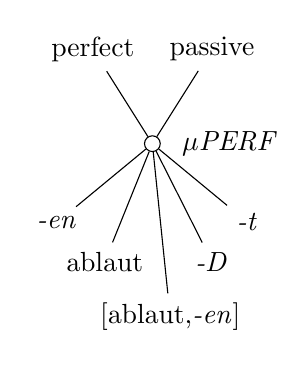
\begin{tikzpicture}[draw=black!100]
 	%[shorten >=1pt,->,draw=black!100]
	\def \rowatticone{4.0cm}
 	\def \rowtwoht{3.5cm}
	\def \rowtwohta{3.2cm}
 	\def \rowoneht{2cm}
	\def \rowzerohta{0.8cm}
	\def \rowzeroht{0.5cm}
	\def \basementone{0.0cm}
 	\tikzstyle{ms-node}=[text centered]
 	\tikzstyle{m-node}=[circle,draw=black!100,thin,inner sep=0pt,minimum size=2mm]
	\tikzstyle{pf-node}=[text centered]
 	\tikzstyle{m-lbl}=[text width=5ex]
	\node[m-lbl] (label0) at (13ex,\rowoneht) {$\mu{\textit{PERF}}$};
	
 	% morphosyntax
 	\node[ms-node] 	(ms0)	at (3ex,\rowtwohta)		{perfect};
 	\node[ms-node] 	(ms1)	at (13ex,\rowtwohta)	{passive};
	
 	% morphome
 	\node[m-node] 	(m0)	at (8ex,\rowoneht)		{};
	
	%phonological form
	 \node[pf-node] 	(pf0)	at (0ex,1cm)		{\textit{-en}};
 	\node[pf-node]  	(pf1)	at (4ex,\rowzeroht)		{ablaut};
 	\node[pf-node]  	(pf2)	at (9.5ex,-0.2cm)	 	{[ablaut,\textit{-en}]};
 	\node[pf-node]  	(pf3)	at (13ex,\rowzeroht) 		{\textit{-D}};
 	\node[pf-node] 	(pf4)	at (16ex,1cm) 		{\textit{-t}};	
	
 	\path (pf0)	edge	node	{}	(m0)
 		(pf1)	edge	node	{}	(m0)
 		(pf2)	edge	node	{}	(m0)
 		(pf3)	edge	node	{}	(m0)
		(pf4)	edge	node	{}	(m0)
		(m0) edge node 	{}	(ms0)
		(m0) edge node 	{}	(ms1);
		%(label0) edge node {}      (m0);	
 \end{tikzpicture}
\label{fig:ppgraph}
\caption{In the terminology of \cite{aronoff}, the \ac{EN} \ac{perf-ptc}  is a \emph{polyvalent polymorphous} morphome; i.e., it has multiple functions (polyvalent) as well as multiple forms (polymorphous). The downward arcs represent form types, each of which is a \emph{meromorphomes.}}
\end{figure}

%\begin{figure}[ht]
%\centering
%%Monovalent monomorphous
%\subfigure[\label{fig:mtypes:mvmm}]{
%     \begin{tikzpicture}[draw=black!100]
% 	%[shorten >=1pt,->,draw=black!100]
%	\def \rowatticone{4.0cm}
% 	\def \rowtwoht{3.5cm}
%	\def \rowtwohta{3.2cm}
% 	\def \rowoneht{2cm}
%	\def \rowzerohta{0.8cm}
%	\def \rowzeroht{0.5cm}
%	\def \basementone{0.0cm}
% 	\tikzstyle{ms-node}=[text centered]
% 	\tikzstyle{m-node}=[circle,draw=black!100,thin,inner sep=0pt,minimum size=2mm]
%	\tikzstyle{pf-node}=[text centered]
% 	\tikzstyle{m-lbl}=[text centered]
%	\node[m-lbl] (morphome-label) at (5ex,\rowoneht) {$\mu{\textit{MENT}}$};
% 	% morphosyntax
% 	\node[ms-node] 	(ms0)	at (0ex,\rowtwoht)		{+noun};
% 	% morphome
% 	\node[m-node] 	(m0)	at (0ex,\rowoneht)		{};
%	%phonological form
%	 \node[pf-node] 	(pf0)	at (0ex,\rowzeroht)		{\textit{-ment}};
%
% 	\path (pf0)	edge	node	{}	(m0)
%		(m0) edge node 	{}	(ms0);		
% \end{tikzpicture}
%} %Monovalent polymorphous
%\subfigure[\label{fig:mtypes:mvpm}]{
%     \begin{tikzpicture}[draw=black!100]
% 	%[shorten >=1pt,->,draw=black!100]
%	\def \rowatticone{4.0cm}
% 	\def \rowtwoht{3.6cm}
%	\def \rowtwohta{3.2cm}
% 	\def \rowoneht{2cm}
%	\def \rowzerohta{0.8cm}
%	\def \rowzeroht{0.4cm}
%	\def \basementone{0.0cm}
% 	\tikzstyle{ms-node}=[text centered]
% 	\tikzstyle{m-node}=[circle,draw=black!100,thin,inner sep=0pt,minimum size=2mm]
%	\tikzstyle{pf-node}=[text centered]
% 	\tikzstyle{m-lbl}=[text centered]
%	\node[m-lbl] (morphome-label) at (12ex,\rowoneht) {$\mu{\textit{PAST}}$};
%	
% 	% morphosyntax
% 	\node[ms-node] 	(ms0)	at (7.5ex,3.0cm)		{past};
%	
% 	% morphome
% 	\node[m-node] 	(m0)	at (7.5ex,\rowoneht)		{}; %{$\mu{\textit{EN}}$};
%	
%	%phonological form
%	 \node[pf-node] 	(pf0)	at (0ex,\rowzerohta)		{$\emptyset$};
% 	\node[pf-node]  	(pf1)	at (3ex,\rowzeroht)		{\textit{-t}};
% 	\node[pf-node]  	(pf2)	at (7.5ex,\basementone)	 	{ablaut};
% 	\node[pf-node]  	(pf3)	at (12ex,\rowzeroht) 		{\textit{-d}};
% 	\node[pf-node] 	(pf4)	at (15ex,\rowzerohta) 		{\dots};	
%	
% 	\path (pf0)	edge	node	{}	(m0)
% 		(pf1)	edge	node	{}	(m0)
% 		(pf2)	edge	node	{}	(m0)
% 		(pf3)	edge	node	{}	(m0)
%		(pf4)	edge	node	{}	(m0)
%		(m0) edge node 	{}	(ms0);	
% \end{tikzpicture}
%}
%%Polyvalent polymorphous
%\subfigure[\label{fig:mtypes:pvpm}]{
%	\vspace{12pt}
%     \begin{tikzpicture}[draw=black!100]
% 	%[shorten >=1pt,->,draw=black!100]
%	\def \rowatticone{4.0cm}
% 	\def \rowtwoht{3.5cm}
%	\def \rowtwohta{3.2cm}
% 	\def \rowoneht{2cm}
%	\def \rowzerohta{0.8cm}
%	\def \rowzeroht{0.5cm}
%	\def \basementone{0.0cm}
% 	\tikzstyle{ms-node}=[text centered]
% 	\tikzstyle{m-node}=[circle,draw=black!100,thin,inner sep=0pt,minimum size=2mm]
%	\tikzstyle{pf-node}=[text centered]
% 	\tikzstyle{m-lbl}=[text width=5ex]
%	\node[m-lbl] (label0) at (13ex,\rowoneht) {$\mu{\textit{EN}}$};
%	
% 	% morphosyntax
% 	\node[ms-node] 	(ms0)	at (3ex,\rowtwohta)		{perfect};
% 	\node[ms-node] 	(ms1)	at (13ex,\rowtwohta)	{passive};
%	
% 	% morphome
% 	\node[m-node] 	(m0)	at (8ex,\rowoneht)		{};
%	
%	%phonological form
%	 \node[pf-node] 	(pf0)	at (0ex,1cm)		{\textit{-en}};
% 	\node[pf-node]  	(pf1)	at (4ex,\rowzeroht)		{ablaut};
% 	\node[pf-node]  	(pf2)	at (9.5ex,-0.2cm)	 	{[ablaut,\textit{-en}]};
% 	\node[pf-node]  	(pf3)	at (13ex,\rowzeroht) 		{\textit{-D}};
% 	\node[pf-node] 	(pf4)	at (16ex,1cm) 		{\textit{-t}};	
%	
% 	\path (pf0)	edge	node	{}	(m0)
% 		(pf1)	edge	node	{}	(m0)
% 		(pf2)	edge	node	{}	(m0)
% 		(pf3)	edge	node	{}	(m0)
%		(pf4)	edge	node	{}	(m0)
%		(m0) edge node 	{}	(ms0)
%		(m0) edge node 	{}	(ms1);
%		%(label0) edge node {}      (m0);	
% \end{tikzpicture}
% }
%% Polyvalent monomorphous
%\subfigure[\label{fig:mtypes:pvmm}]{
%     \begin{tikzpicture}[draw=black!100]
%	\def \rowatticone{4.0cm}
% 	\def \rowtwoht{3.5cm}
%	\def \rowtwohta{3.2cm}
% 	\def \rowoneht{2cm}
%	\def \rowzerohta{0.8cm}
%	\def \rowzeroht{0.5cm}
%	\def \basementone{0.0cm}
% 	\tikzstyle{ms-node}=[text centered]
% 	\tikzstyle{m-node}=[circle,draw=black!100,thin,inner sep=0pt,minimum size=2mm]
%	\tikzstyle{pf-node}=[text width=12ex, text centered]
% 	\tikzstyle{m-lbl}=[text width=5ex]
%	\node[m-lbl] (label) at (11ex,1.5cm) {$\mu{Z}$};
%	
% 	% morphosyntax
%	 \node[ms-node] 	(ms0)	at (0ex,2.5cm)			{clitic};
% 	\node[ms-node]  	(ms1)	at (4ex,3.2cm)		{poss.};
% 	\node[ms-node]  	(ms2)	at (9 ex,3.2cm)	 	{n.pl};
% 	\node[ms-node]  	(ms3)	at (13ex,2.5cm) 		{v.3sg};
% 	% morphome
% 	\node[m-node] 	(m0)	at (6ex,1.5cm)		{};
%	
%	%phonological form
% 	\node[pf-node]  	(pf0)	at (6ex,0.0cm)	 	{\textit{-Z}};
%
% 	\path (pf0)	edge	node	{}	(m0)
% 		(m0)	edge	node	{}	(ms0)
% 		(m0)	edge	node	{}	(ms1)
% 		(m0)	edge	node	{}	(ms2)
%		(m0)	edge	node	{}	(ms3);
%		%(label)  edge  node {}     (m0);		
% \end{tikzpicture}
%}
%\caption[]{Round's is not the only morphome taxonomy. \cite{aronoff:md:2016} classifies morphomes by complexity. 
%Subfigure \subref{fig:mtypes:mvmm} represents the  
%\textbf{monovalent monomorphous} type, 
%\subref{fig:mtypes:mvpm} the \textbf{monovalent polymorphous} type, 
%\subref{fig:mtypes:pvpm} the \textbf{polyvalent polymorphous} type, 
%and \subref{fig:mtypes:pvmm} the \textbf{polyvalent monomorphous} type. (This 
%diagram is a reproduction of the one in \cite{aronoff:md:2016}.) } 
%\label{fig:mtypes}
%\end{figure}

\paragraph{Meromorphomes.} Whereas rhizomorphomes and metamorphomes 
transcend the realms of individual lexemes and paradigms and thus highly 
abstract, meromorphomes are comparatively concrete, as they 
correspond to particular parts of word forms. Meromorphomes, it must be said, 
are not the word parts themselves, since all morphomes reside at the 
morphomic level rather than the phonological, or surface, level \citep{round:2011}. 
Even so, meromorphomes map directly onto phonological forms, and 
are thus more closely associated with phonological forms than rhizomorphomes 
or metamorphomes. Indeed, both rhizomorphomes and metamorphomes are 
composed of meromorphomes, since, at some point, the abstract, trans-lexemic 
types of morphomes must interact with specific phonological forms. 

For instance, in \ac{EN} \ac{perf-ptc}s, each individual root, e.g., \textit{s-ng}, 
\textit{br-k}, \textit{kick}, etc., is a meromorphome. Each suffix 
as well as each particular variety of ablaut is also a meromorphome. 
The Romance L-morphome is also composed of particular meromorphomes. 
Within the paradigm of the lexeme \textsc{decir} \textsc{`to say'} 
(table \ref{tab:l-morphome}). The stem \textit{dig-} is a meromorphome. 
Similarly, the stem \textit{crezc-} is a meromorphome within the paradigm of 
\textsc{crecir} \textsc{`to grow'}.

\begin{table}[ht]
\begin{center}
\subtable[maqomi `local' \label{subtab:fusion:1}]{
\setlength{\extrarowheight}{8pt}
{\begin{tabular}{lcc}
\  & masc & fem  \\
\hline 
sg & maqom-i & meqom-i-t  \\
pl & meqom-iy-im & meqom-iy-ot  \\
\end{tabular}}
}
\subtable[gadol `big' \label{subtab:fusion:2}]{
\setlength{\extrarowheight}{8pt}
{\begin{tabular}{lcc}
\  & masc & fem  \\
\hline 
sg & gadol & gdol-a  \\
pl & gdol-im & gdol-ot  \\
\end{tabular}}
}
\label{tab:fusion}
\caption{Fusional suffixes in Hebrew nominals}
\end{center}
\end{table}

\subsection{An example from Hebrew}
\label{sec:heb-example}
We turn now to a case of syncretism in the morphology of \ac{MH}. Perhaps
the best known aspect of Hebrew (and Semitic languages in general) is its 
non-concatenative root-and-pattern morphology. But 
Hebrew's morphology also has a rich concatenative component, consisting of
of both inflectional and derivational affixes. Moreover, the inflectional affixes tend to be
highly (and idiosyncratically) fusional.  
Consider the forms in table~\ref{tab:fusion}. 

In this section, we shall primarily be concerned with the
interaction between \textit{-t} and \textit{-i} in Hebrew feminine endings.
Hebrew uses the vowel [i] 
in both noun-deriving and adjective-deriving suffixes. 
As illustrated in table~\ref{subtab:der-adjectives}, 
one can derive adjectives 
in Hebrew by attaching \textit{-i} to noun bases. The \textit{-i} 
must be the `adjective' exponent
in table \ref{subtab:der-adjectives} because it is the only suffixal 
element to occur in each
of the four columns. % It must therefore be the adjectival exponent in these cases. 
\begin{table}[ht]
   \centering
   \caption{Derivational and inflectional syncretism in Hebrew feminine endings.}\label{tab:deriv} 
   \subtable[Adjectives derived from nouns via \textit{-i}\label{subtab:der-adjectives}]{
     \centering
     \setlength{\extrarowheight}{8pt}
        \begin{tabular}{l l l l c}
       \toprule
        \textsc{noun base} &  \textsc{masc.sg} & \textsc{fem.sg} &  \textsc{fem.pl} & \textsc{gloss} \\ %[0.5ex]
        \midrule
        %tarbut \textit{`culture'} & tarbut-i & tartbut-i-t & tarbut-iy-ot & `cultured' \\
        %le\textipa{P}om \textit{`nation'} & le\textipa{P}omi & le\textipa{P}omit & le\textipa{P}omiyot  & `national' \\
        merxav \textit{`space'} & merxav-i  &  merxav-i-t  &  merxav-iy-ot   &  `spatial' \\
        \textipa{P}aviv \textit{`spring'} & \textipa{P}aviv-i & \textipa{P}aviv-i-t & \textipa{P}aviv-iy-ot  & `spring-like' \\
        \textipa{P}arec \textit{`land'} & \textipa{P}arc-i & \textipa{P}arc-i-t & \textipa{P}arc-iy-ot  & `earthly' \\
        \bottomrule 
    \end{tabular}
   }\\
\vspace{6pt}
      \subtable[Nouns derived via \textit{-it}\label{subtab:der-nouns-i}]{
      \setlength{\extrarowheight}{8pt}
     \centering
     
    \begin{tabular}{l l l c} % creating 3 columns
   \toprule
    \textsc{base} &  \textsc{sg} &  \textsc{pl} & Gloss \\ 
    \midrule
    %pax \textit{`tin'} & pax-it & pax-iy-ot & `tin can' \\
    ma\d{s}a\textipa{P} `cargo' & ma\d{s}a\textipa{P}-it  &   ma\d{s}a\textipa{P}-iy-ot  &   `truck'   \\
    xalal \textit{`space'} & xalal-it & xalal-iy-ot & `spaceship' \\
    %k.r.k \textit{`(to) wrap'} &  kru\d{k}-it   &   kru\d{k}iy-ot  & `strudel' \\ %(iff \textit{fem}) or \\
    nagar \textit{`carpenter'}  &  nagar-it   &   nagr-iy-ot  & `female carpenter' \\
    \bottomrule
    \end{tabular}
   }\\
   \vspace{6pt}
   \subtable[Nouns derived via \textit{-ut}\label{subtab:der-nouns-u}]{
   \setlength{\extrarowheight}{8pt}
     \centering
        \begin{tabular}{l l l c}
        \toprule
        \textsc{base} &  \textsc{sg} &  \textsc{pl} & \textsc{gloss} \\ %[0.5ex]
        \midrule
        ma\v{s}ma\textrevglotstop \textit{`meaning'} & ma\v{s}ma\textrevglotstop-{u}t & ma\v{s}ma\textrevglotstop-{u}y-ot & `importance' \\
	\v{s}agrir \textit{`ambassador'} & \v{s}agrir-ut & \v{s}agriruy-ot & `embassy' \\
        %b.g.r \textit{`(to) mature'}  &  bagr-ut  &  bagr-uy-ot  &  `matriculation exam' \\
        nagar \textit{`carpenter'} &  nagar-ut   &   nagr-uy-ot  & `carpentry' \\
        \bottomrule
	\end{tabular}
   }
%\caption{Subtable (\ref{subtab:der-adjectives}) presents several adjectives 
%that are derived from nouns via the %adjective-deriving 
%\textit{-i} suffix. 
%Feminine adjectives are formed by attaching \textit{-t} to the \textit{-i} of the masc. form. Subtable 
%(\ref{subtab:der-nouns-i}) shows a different suffixal function of \textit{-i}, but here it is used 
%in conjunction with \textit{-t} to derive nouns instead of adjectives. Finally, 
%subfigure (\ref{subtab:der-nouns-u}) illustrate another nominalization suffix, 
%namely \text{-u.}}
%Realizations of the morphomes $\mu$\textsc{i}, $\mu$\textsc{t}, $\mu$\textsc{o}, and $\mu$\textsc{u} in the suffixes
%\textit{-i(t)}, \textit{-it}, \textit{-ot}, and \text{-ut}.}
\end{table}
Thus, \textit{merxav} `space' + \textit{-i} = \textit{merxav-i} 
`spatial (masc.sg)'. The fem.sg is obtained by attaching \textit{-t} to the masc.sg
form. Feminine adjectives thus end in \textit{-it}. 
Hebrew also uses \textit{-it} to derive nouns, usually by attaching it 
to nouns, as in in table~\ref{subtab:der-nouns-i}. 
The vast majority of nouns derived in this way are feminine in 
grammar, semantics, or both. 

%When used to
%derive nouns, \, i.e., feminine , usually from 
%other nouns, by attaching the suffix \textit{-it} to the base, 
%as in table \ref{subfig:der-nouns-i}. 

%However, the ending \textit{-it} also occurs
%in the derived adjectives subtable, but in this case
%it is composed of two suffix. %It is evident that 
%The \textit{-i} is the common adjective-deriving 
%unit across the table's columns, since it is the 
%difference between each base base and 
%its corresponding form in the \textit{masc.sg} adjective 
%column  (e.g., \textit{merxav} `space' ~ \textit{merxav-i} 
%`spatial')

%\begin{table}[h]
%\centering % centering table
%\begin{tabular}{c c c c c c} % creating 3 columns
%\hline\hline %inserting double-line
%Lexical cat. & Lexeme &\textsc{m.sg} & \textsc{f.sg} &  \textsc{m.pl} & \textsc{f.pl}\\ [0.5ex]
%\hline % inserts single-line
%Adjectives & \textsc{local} & maq\'om &   maqom\'i   &  mqom\'it   &   mqomiyi\'ot \\
%	&	& maqom & maqom+$\mu${\textsc{adj}} & maqom+$\mu${\textsc{adj}}+$\mu${\textsc{t}} & maqom+$\mu${\textsc{adj}}+$\langle \mu${\textsc{o}}-$\mu$\textsc{t} $\rangle$ \\
%	&	& \textsc{maqom} & \textsc{maqom}+\textsc{adj}+\textsc{m.pl} & \textsc{maqom}+\textsc{adj}+\textsc{f.sg}  & \textsc{maqom}+\textsc{adj}+\textsc{f.pl} \\
%Participles & \textsc{tell} & mesap\'er & mesapr\'im  & mesap\'eret &  mesapr\'ot\\
%	&	& mesaper & mesaper+$\mu${\textsc{adj}} & mesaper+$\mu${\textsc{adj}}+$\mu${\textsc{t}} & mesaper+$\mu${\textsc{adj}}+$\langle \mu${\textsc{o}}-$\mu$\textsc{t} $\rangle$ \\
%	&	& \textsc{mesaper} & \textsc{s.p.r}+\textsc{adj}+\textsc{m.pl} & \textsc{mesaper}+\textsc{adj}+\textsc{f.sg}  & \textsc{mesaper}+\textsc{adj}+\textsc{f.pl} \\
%\hline % inserts single-line
%\end{tabular}
%\label{tab:hresult}
%\caption{Performance Using Hard Decision Detection} %title of the table
%\end{table}

%\begin{figure}[h]
%\begin{center}
%\subfigure[Adjectives derived via +\textit{i}\label{subfig:der-adjs-i}]{
%\begin{tabular}{c c c c c c} % creating 3 columns
%%\centering % centering table
%%\caption{Derived Adjectives.}\label{tab:hresult}
%\toprule%inserting double-line
%\textsc{noun base} &  \textsc{masc.sg} & \textsc{fem.sg} &  \textsc{fem.pl} & Gloss \\ [0.5ex]
%\midrule
%tarbut (`culture') & tarbuti & tartbutit & tarbutiyot & `cultured' \\
%le\textipa{P}om (`nation') & le\textipa{P}omi & le\textipa{P}omit & le\textipa{P}omiyot  & `national' \\
%merxav (`space') & merxavi & merxavit & merxaviyot  & `spatial' \\
%\textipa{P}aviv (`spring') & \textipa{P}aviv i & \textipa{P}aviv it & \textipa{P}aviviyot  & `spring-like' \\
%le\textipa{P}arec (`land') & le\textipa{P}arci & le\textipa{P}arcit & le\textipa{P}arciyot  & `earthly' \\
%\bottomrule % inserts single-line
%%\label{subfig:der-adjs-i}
%\end{tabular}
%} \\
%\subfigure[Nouns derived via \label{subfig:der-nouns-i}]{ %+\textit{i}]{
%\begin{tabular}{c c c c} % creating 3 columns
%\hline
%\textsc{base} &  \textsc{sg} &  \textsc{pl} & Gloss \\ [0.5ex]
%\hline
%pax (`tin') & paxit & paxiyot & `cultured' \\
%ma\d{s}a\textipa{P} (`load') & ma\d{s}a\textipa{P}it  &   ma\d{s}a\textipa{P}iyot  &   `truck'   \\
%$\sqrt{\text{k.r.k}}$ (`bind, wrap')  &  kru\d{k}it   &   kru\d{k}iyot  & `strudel' (iff \textit{fem}) or `@' (iff \textit{masc}) \\
%nagar (`carpenter')  &  nagarit   &   nagriyot  & `female carpenter'
%\hline % inserts single-line
%%\label{subfig:der-nouns-i}
%\end{tabular}
%}  
%\subfigure[Nouns derived via +\textit{u}\label{subfig:der-nouns-u}]{
%\begin{tabular}{c c c c}
%\textsc{base} &  \textsc{sg} &  \textsc{pl} & Gloss \\ [0.5ex]
%\midrule
%\v{s}agrir (`ambassador') & \v{s}agrirut & \v{s}agriruyot & `embassy' \\
%$\sqrt{\text{b.g.r}}$  (`mature') &  bagrut & bagruyot &  `matriculation exam' \\
%nagar (`carpenter')  &  nagarut   &   nagruyot  & `carpentry'
%\bottomrule %maiden:2005 inserts single-line
%%\label{subfig:der-nouns-u}
%\end{tabular}
%} 
%\end{center}
%\caption{The \textit{t} quasi-morpheme}
%\label{fig:t}
%\end{figure}
In Hebrew, feminine words frequently 
end in \textit{-t}. Indeed, the co-occurrence of \textit{-t} and the feminine gender is 
too frequent to be the product of random chance \citep{faust:2013}.
In fact, \textit{-t} serves as an exponent of both grammatical (or \emph{inflectional}) 
gender as well as semantic (or \emph{derivational}) gender. For example, /-t/ 
is an inflectional ending in \textit{merxavit} `spatial (fem.)' 
(cf. the corresponding masc. form \textit{merxavi}). 
It is as part of the derivational suffix \textit{-it}, used to 
derive semantically feminine nouns, in \textit{nagar-it} 
`female carpenter' (cf. \textit{nagar}`(male) carpenter'). 
Tables~\ref{subtab:der-adjectives} and \ref{subtab:der-nouns-i} 
show additional
examples of these two disparate functions of \textit{-i}.

\subsection{A morpheme-based approach}
The ending \textit{-t}, when used as (part of) a suffix on 
nominal forms, is always accompanied by a vowel. 
In fact, it appears with each of Modern Hebrew's five vowels.
In singular-form endings, it appears with every vowel except 
\textit{o}: \textit{-at}, \textit{-(e)t}, \textit{-ut}, and \textit{-it}. 
It appears with \textit{o} in the feminine plural suffix \textit{-ot} 
also ends with \textit{t}. \footnote{The consonant /t/ occurs with 
/o/ in singular forms as well, but only when /-ot/ is part of a 
primitive word, as in, e.g., \textipa{P}ot `letter'.}

Besides \textit{-t}, the only other systematic feminine marker is 
\textit{-a}, which is found only 
in fem.sg absolute-state forms. [Examples]
But a final \textit{-t} appears even in these nouns when they are 
in the construct state, a type of form which is used compound-noun 
construction and marked by its complete lack of stress.
\cite{schwarzwald:1982} argues that
the construct-state's \textit{t} ending was once also 
present on the absolute \textit{-a}, but was lost through a historical
\textit{t-}deletion process. \cite{faust:2013}, however, 
goes a step further, arguing that the \textit{t} remains 
underlyingly present in \textit{-a} even today. According 
to \cite{faust:2013}, both
\textit{-a} and \textit{-t} are underlyingly /-at/; sometimes 
the \textit{a} deletes, and sometimes the \textit{-t} deletes, depending 
upon certain phonological factors. Sometimes they appear 
together in the same form, as in fem.sg construct nouns
Faust additionally decomposes the derivational endings 
\textit{-ut} and \textit{-it} into /u-at/ and /i-at/, respectively. 
The \textit{a} deletes in these forms.
%\cite{faust:2013} thus analyzes the \textit{t} as the universal feminine morpheme of Hebrew\footnote{Faust
%takes an approach based on Distributed Morphology (DB) \cite{halle-and-marantz:1993}, a \emph{morpheme}-based 
%approach.}. Faust moreover decomposes the suffixes \textit{-it}, and \textit{-ut} each into
%two morphemes: the feminine /t/ and /i/, and /u/, respectively. (
%(The suffixes \textit{-et} in \textit{-at} are  regarded 
%by Faust as allophonic.) 
Faust regards \textit{-et} in \textit{-at} as both allophones of /-at/. 
Faust's analysis of the Hebrew feminine endings thus constitutes a total of 
four morphemes, namely /-i/, /-u/, /-at/, and /-o/.

%In the remainder of this discussion, we shall be primarily concerned with /i/, which particularly interesting because
%there seem to be two distinct morphological units /i/.

%\cite{faust:2013} analyzes the Modern Hebrew feminine 
%%In any case, he latter was lost 
%%``through a process of final \textit{t}deletion in absolute state forms" (p. 159). 
%that the current that the modern \textit{-a} ending 
%absolute \cite{schwarzwald:1982, faust:2013} lists the following as the set 
%of possible feminine endings in 
%
%Faust argues that the suffix \textit{-at} is a \emph{root} is such that it selects for another root as its complement. 
%That is, it will only attach to another morpheme of root status
 

%Faust argues that the suffix \textit{-at} is such that it selects for another root as its complement. That is, it will only attach to another morpheme of root status. Note that root here is the technical term of Distributed Morphology \cite{}, not necessarily the consonantal root of Semitic languages, although consonantal roots would certainly be a subset of \ac{DM} roots. 
  
   \begin{table}
     \centering
%        \begin{tabular}{l l c }
%       \toprule
%        \textsc{Morphome} &  Phon. & \\ [0.5ex]
%        \midrule
%       \textsc{fem} & $\mu{\textsc{a}}$ & $\Phi_{\text{A}}$ & {/\'a/, /-at/} \\
%       \textsc{base}$\to${adj}, \textsc{base}$\to$\textsc{noun} &$\mu{\textsc{i}}$ & $\Phi_{\textsc{i}}$ & {/+i/, /+it/} \\
%       $\mu{\textsc{a}}$ & $\mu{\textsc{u}}$ & $\Phi_{\text{U}}$  & {/-ut/} \\
%       $\mu{\textsc{a}}$ & $\mu{\textsc{o}}$ & $\Phi_{\text{O}}$ & {/-ot/}  \\
%       $\mu{\textsc{a}}$ & $\mu{\textsc{t}}$ & $\Phi_{\text{T}}$ & {/-ot/, /-t/} \\
%        \bottomrule 
%    \end{tabular}
\setlength{\extrarowheight}{8pt}
       \begin{tabular}{c c c }
       \toprule
        \textsc{Morphome} &  Phon. suffixe(s) & Morphosyntactic property set(s) \\ [0.5ex]
        \midrule
       $\mu{\textsc{a}}$ & {/-\textbf{a}/},{/-\textbf{a}t/} & \{fem, sg,\textsc{state:}abs\}, \{fem, sg, \textsc{state:}constr\}\\
       $\mu{\textsc{i}}$ & {/-\textbf{i}/, /-\textbf{i}t/} & \text{n}$\to${adj}, \text{n}$\to$\text{n}[fem] \\
       $\mu{\textsc{u}}$ & {/-\textbf{u}t/} & \text{n}$\to$\text{n}[fem, -concrete] \\
       $\mu{\textsc{o}}$ & {/-\textbf{o}t/} & \{fem, pl\} \\
       $\mu{\textsc{t}}$ & { /-\textbf{t}/, /-o\textbf{t}/, /-u\textbf{t}/, /-i\textbf{t}/}  & \{fem\}, \{fem, pl\}, \{fem, -concrete\}, \\
        \bottomrule 
    \end{tabular}
     \label{tab:heb-morphomes}
    \caption{Morphomic and Phonological Operations}
    \end{table}
    
Faust's approach is based on Distributional Morphology 
 \citep{halle-and-marantz:1993}, 
a morpheme-based, Lexical-Realizational theory \citep{stump:2001}
According to Faust, therefore, the suffixes /-i/, /-u/, and /-at/ are not only morphemes, 
but \emph{roots.}
In \ac{DM}, the term \emph{root} (along with \emph{formative}) is used to refer 
to maximally primitive units of meaning. (It is not to be confused with the 
consonantal root of Semitic morphology. Semitic roots would qualify as 
\ac{DM} roots, but the \ac{DM} root is more general than the Semitic root.)
A \ac{DM} root has no particular morpho properties and thus belongs to 
no morphosyntactic category.
However, it does have abstract semantic features as well as inherent 
selectional requirements, i.e., criteria that limit the set of stems with which it 
may combine. In particular, roots exclusively select 
other roots as their complements. %That is to say, roots combine only with roots.  

Because \textit{-at} is a root, therefore, it
never attaches to derived stems. The same is true of /-i/ and /-u/.  
However, \textit{-at} is distinguished from /-i/ and /-u/ in that it occupies the 
position of category head in the derivation of adjectives.
Of course, the suffix /-at/ is not present in the derivations of 
masculine adjectives, 
but the position of category head is. 
It is just phonologically null, according to \ac{DM}.
In such cases, the suffix /-i/ simply combines with the null adjectival head. 
This, according to Faust, satisfies the selectional requirements of /-i/
and the null adjectival head. The rest of the derivation,
proceeds as it does in feminine adjectives. 

%is a root that will attach only to another root. Faust argues that it never attaches to bases that are derived words or loanwords. (The latter, Faust supposes, have a derived status by virtue of the borrowing process. By contrast, -i- and -u- frequently combine with non-roots. 
According to Faust, \textit{-at} sometimes uses \textit{-i} and 
\textit{-u} as buffers. That is, it first attaches to \textit{-i} or \textit{-u}, 
thus forming complex units, either \emph{-it} or \emph{-ut}, respectively, 
which then attach to
the non-primitive stem. Because \emph{-it} and \emph{-ut} are complex, 
they cannot be roots and are thus free of roots' selectional constraints.

%That is, they first attach to
%-i- or -u-, thus forming -it or -ut (the a is deleted), which can then attach to any base, including all manner of derived bases. 

Moreover, Faust argues that the adjectival \textit{-i} and 
the noun-deriving \textit{-i} ending in tables 
\ref{subtab:der-adjectives} and \ref{subtab:der-nouns-i} 
are in fact one and the same expletive morpheme. That is, 
/-i/ does not per se mean `\textsc{adjective}' in the derived adjectives 
\ref{subtab:der-adjectives}. It is rather an expletive suffix, one that 
crucially, for Faust, lacks morphosyntactic properties.
%The seemingly noun-deriving
%suffix \textit{-i} is, according to Faust, the same expletive root. 
Note that it is \ac{DM} that motivates Faust's decision to posit a single 
expletive /-i/ morpheme (as opposed to 
separate adjective-deriving and noun-deriving morphemes).  Faust 
requires /-i/ to be a \ac{DM} root so that /-at/ can combine with it, and since 
\ac{DM} roots must be free of any specification of morphosyntactic 
category, an intrinsically adjectival /-i/ would
not suit Faust's \ac{DM} analysis. 

%If /-i/
%If there were an (intrinsically) adjective-deriving /-i/, it would occupy 
%the position of adjectival head within the word-internal syntax
%and thus could not be a \ac{DM} root.  
%Note also that a more conventional 
%morpheme-based analysis would likely conclude that there are 
%two separate morphemes 
%here, namely two /-i/ suffixes that are identical 
%in form, but distinct in meaning. 


\subsection{A \emph{morphome}-based approach}
As it turns out, Faust's account and a \emph{morphome}-based approach 
are similar top each other in at least one respect, namely in the analysis of /-i/
as a single (unified) morphological unit. But whereas Faust posits a unified 
/-i/ morpheme, we shall posit here a 
a unified \emph{morphome} $\mu{\textsc{i}}$. Like Faust's expletive /-i/,
$\mu{\textsc{i}}$ has no meaning in and of itself, but this is not 
because $\mu{\textsc{i}}$ is entirely unassociated with meaning; 
$\mu{\textsc{i}}$ lacks intrinsic meaning because meaning is not the 
purview of a morphomic representation. Rather, meaning is supplied by 
the lexical level. One of the advantages of a morphomic approach
is that any number of different meanings can be mapped onto a single 
morphome. We shall also posit a morphome corresponding to the 
feminine ending \textit{-a} and a \emph{different} morphome for 
\textit{-t}, as there does not seem to be enough synchronic evidence to posit that 
\textit{-a} and \text{-t} both have the \emph{synchronic} 
underlying form /-at/.
 \begin{figure}[ht]
  \small
\begin{center}
    \label{tab:heb-morphomic-analyses} 
   \subfigure[{\textglotstop}{avavit} `spring-like'\label{subtab:heb-avivit}]{
     \centering
     \setlength{\extrarowheight}{8pt}
        \begin{tabular}{l c c c}
       \toprule
        \multicolumn{4}{c}{[\textipa{P}avivit] `spring-like'}\\
        \midrule
        \multirow{2}{*}{Phonological} & \textipa{P}aviv & -i & -t \\ %\hline
         %& $\Phi{\textsc{stem}} (\text{a.i}, \text{\textipa{P}.b.b} )$ & $\Phi_{\textsc{i}}$ & $\Phi_{\textsc{t}}$ \\ %\hline
         %& $\Phi{\textsc{stem}} (\text{a.i}, \textsc{\textipa{P}bb})$ & $\Phi{\textsc{i}}$ & $\Phi{\textsc{t}}$ \\
         & $\Phi${\textsc{stem}} & $\Phi${\textsc{i}} & $\Phi${\textsc{t}} \\
       Morphomic & $\mu$\textsc{a-i}, $\surd \textsc{\textipa{P}-b-b}$ & $\mu{\textsc{i}}$  & $\mu{\textsc{t}}$ \\ 
        Lexical & \multicolumn{3}{c}{$\surd \textsc{\textipa{P}-b-b}$, \{\text{adj}, \text{fem}, \text{sg}\}}\\
        \bottomrule 
    \end{tabular}
    }
%      \vspace{7pt}
%   \subtable[xalalit `spaceship'\label{subtab:heb-xalalit}]{
%     \centering
%        \begin{tabular}{l r}
%       \toprule
%        \multicolumn{2}{c}{xalalit}\\
%        \midrule
%        \multirow{2}{*}{Phonological} & xalal-it \\ %\hline
%         %& $\Phi_{\textsc{stem}}$ %( \textipa{a.a}, \text{\textipa{x.l.l}} )$ 
%        & $\Phi{\textsc{it}}$, $\Phi_{\textsc{stem}}$ \\ %\hline
%        Morphomic & $\mu{\textsc{t}}$, $\mu{\textsc{i}}$, $\mu{\textsc{\textipa{a.a}}}$, $\surd \text{xll}$\\ %\hline
%        Lexical & $\surd \textsc{xll}$, \{\text{noun}, \text{fem}, \text{sg}\} \\
%        \bottomrule 
%    \end{tabular}
%    }
    \vspace{6pt}
      \subfigure[xalalit\label{subtab:heb-xalalit}]{
     \centering
     \setlength{\extrarowheight}{8pt}
    \begin{tabular}{l c c}
       \toprule
          \multicolumn{3}{c}{[xalalit] `spaceship'}\\
        \midrule
          \multirow{2}{*}{Phonological} & xalal & -it \\
           & $\Phi$\textsc{stem} & $\Phi$\textsc{it} \\
           Morphomic & $\mu$\textsc{a.a}, $\surd$\textsc{x-l-l} & $\mu$\textsc{i}, $\mu$\textsc{t} \\ 
            Lexical & \multicolumn{2}{c}{$\surd$\textsc{x-l-l}, \{\text{noun}, \text{fem}, \text{sg}\}}\\
       \bottomrule 
    \end{tabular}
    }
%      \vspace{7pt}
%  \subtable[\textglotstop{aviviyot}\label{subtab:heb-aviviyot}]{
%    \centering
%        \begin{tabular}{l c c c}
%       \toprule
%       % //\textsc{noun base} &  \textsc{masc.sg} & \textsc{fem.sg} \\ [0.5ex]
%        \multicolumn{5}{c}{\textipa{P}aviviyot `spring-like (\textsc{pl})}\\
%        \midrule
%        \multirow{2}{*}{Phonological} & \textipa{P}aviv & i & ot \\ %\hline
%         & $\Phi_{\textsc{stem}}$ 
%         %s( \text{a.i}, \text{\textipa{P}.b.b} )$ 
%         & $\Phi_{\textsc{i}}$ & $\Phi_{\textsc{ot}}$ \\ %\hline
%        Morphomic & $\mu{\text{a.i}}$, $\surd \text{\textipa{P}bb}$ & $\mu{\textsc{i}}$  & \multicolumn{2}{c}{$\mu{\textsc{o}}$, $\mu{\textsc{t}}$} \\ %\hline
%        Lexical & \multicolumn{4}{c}{$\surd \text{\textipa{P}bb}$, \{\textsc{+adj}, \textsc{+fem}, \textsc{+pl}\}}\\
%        %$\mu{\textsc{t}}$ & $\Phi_{\text{T}}$ & {/t/} \\
%        \bottomrule 
%    \end{tabular}
          \vspace{6pt}
  \subfigure[xalaliyot `spaceships'\label{subtab:heb-xalaliyot}]{
  \setlength{\extrarowheight}{8pt}
    \centering
        \begin{tabular}{l c c c }
       \toprule
       % //\textsc{noun base} &  \textsc{masc.sg} & \textsc{fem.sg} \\ [0.5ex]
        \multicolumn{4}{c}{[\textipa{x}alaliyot] `spaceships'}\\
        \midrule
        \multirow{2}{*}{Phonological} & xalal & i & ot \\ 
         & $\Phi$\textsc{stem}
         %s( \text{a.i}, \text{\textipa{P}.b.b} )$ 
         & $\Phi$\textsc{i} & $\Phi$\textsc{ot} \\ 
        Morphomic & $\mu${\textsc{a-a}}, $\surd$\textsc{x-l-l} & $\mu$\textsc{i}  &  $\mu$\textsc{o}, $\mu$\textsc{t} \\
                            %\multicolumn{2}{c}{$\mu$\textsc{o}, $\mu$\textsc{t}} \\ %\hline
        Lexical & \multicolumn{3}{c}{$\surd$\textsc{x-l-l}, \{\text{noun}, \text{fem}, \text{pl}\}}\\
        \bottomrule 
       \end{tabular}
  }
    \caption{Morphomic analyses} 
    \end{center}
    \end{figure}
 Finally, we shall posit distinct morphomes for the abstract (-\textsc{concrete}) 
 nominalizing suffix \textit{-u}
 as well as the \textit{-o} in the feminine plural \textit{-ot}.
That is, following \cite{faust:2013}, we shall
decompose not only /-it/, but /-ut/ and /-ot/ as well. 
%the feminine plural \textit{-ot} into \textit{-o} 
%and \textit{-t}, each corresponding to a distinct morphome at the 
%morphomic level.

   
  Accordingly, we need a total of five morphomes
  to account Hebrew's range of feminine suffixes. These are presented in table \ref{tab:heb-morphomes}. 
  Note that the mapping from 
  morphomes to phonological suffixes is not one-to-one. For example, 
  $\mu{\textsc{i}}$ maps to the adjective-deriving suffix /-i/. It also 
  plays a part in the realization of the noun-deriving suffix /-it/. Now, 
  this noun-deriving /-it/ is a single \emph{non-decomposable} suffix at the phonological 
  level. The evidence for this is the fact that the /t/ cannot be detached 
  from the /i/ when /-it/ is serving a noun-deriving purpose. Consider, for 
  example, nagar-it `female carpenter', which is derived from the suffix-less, 
  masculine noun base \emph{nagar} `(male) carpenter'. 
There is no *\emph{nagar-i}.
  
Together, $\mu\textsc{i}$ and $\mu\textsc{t}$ form what is in effect  
a \emph{complex morphome} \citep{round:2015, round:md:2016}. A single 
phonological operation maps $\langle \mu\textsc{i}$, $\mu\textsc{t} \rangle$ 
onto a single morphological unit in the phonological output, namely the 
noun-deriving /-it/. The formation of the complex morphome $\langle \mu\textsc{i}$, 
$\mu\textsc{t} \rangle$ is conditioned upon presence of the 
property \{\text{n}$\to$\text{n}[fem] among the derivational properties $\delta$.
 
% The reason we want this pair 
% of morphomes to map to a monolithic phonological representation
% %important We want the nominalizing /-it/ to be represented at the phonological level as a single suffix because
%is that the /t/ cannot be detached from the /i/ when /it/ is serving the purpose 
%of noun-derivation; the noun-deriving /-it/ is always attached to a masculine noun base
%as a whole. Consider, for example nagar-it `female carpenter', which is derived from 
%the suffix-less, masculine noun base \emph{nagar} `(male) carpenter'. There is no 
% *\emph{nagar-i}.

  By contrast, consider the masc.sg adjective form \emph{\textglotstop{aviv-i}} 
  `spring-like', derived from the \emph{\textglotstop{aviv} `spring'}, 
  as well its feminine-adjective inflection  \emph{\textglotstop{aviv-i-t}}. Here, the /-t/ 
  is very much detachable; its removal simply produces the masculine form. We
  thus regard the feminine adjective ending as decomposable even at the 
  phonological level, and thus there can be no complex morphome $\langle \mu\textsc{i}$, 
  $\mu\textsc{t} \rangle$ at the morphomic level. The same morphomes are present in the 
  morphomic representation of \emph{\textglotstop{aviv-i-t}}, but they are each 
  independently mapped to phonological representations.
  
  It is important that the same morphomes be present in the morphomic 
  representations of both noun-deriving and adjectival instances of /-it/, 
  even if the mappings from morphomes to the phonological level are different. We 
  want to acknowledge that the identities of form are not accidental, 
  and that there is sameness here at some level. The purpose of the 
  morphomic level is to account for
  this sort of sameness.
  
 We shall analyze /-ot/, the fem.pl. suffix, and /-ut/, the abstract (or \textsc{concrete:}[-])
 noun-deriving suffix, in a similar way. Both are monolithic suffixes at the phonological
 level, and both have complex morphomic representations. Again, the primary reason for this
 is that neither /-ot/ nor /-ut/ seem to be decomposable, at least not in a straightforward
 way; that is, /-ot/ as a whole is the fem.pl suffix. If /-t/ is the fem. suffix, then
 /-o/ should be plural suffix. If this were the case, we would expect to see
 /-o/ in the masc.pl. ending, but the masc.pl. suffix is in fact /-im/. The suffix /-ot/
 corresponds to the morphome pair $\langle \mu\textsc{o}$, $\mu\textsc{t} \rangle$, 
 as shown in table \ref{subtab:heb-xalaliyot}, and /-ut/ to $\langle \mu\textsc{u}$, 
 $\mu\textsc{t} \rangle$. Analyzed in this way, /-ot/ and /-it/ share the morphome 
 $\mu$\textsc{t} with /-it/, thus accounting for the fact that all three suffixes end 
 in /-t/. The morphome $\mu\textsc{t}$ is thus used both derivationally and 
 inflectionally, a kind of dual appropriation that is not unknown among the world's languages. 
 Round, for instance, has frequently observed it in Kayardild: ``[M]ost of the exponents 
 employed by the inflectional system are also used derivationally" \citep[][p. 13]{round:2015}.
  
%that is, a morphomic representation separate from both
%the lexical and the phonological levels. We thus allow it to
%be associated with two separate meanings at once. 

%In Hebrew, all category heads are roots, and a root will not combine with a 
%non-root, i.e., non-primitive select for roots exclusively. To derive an adjective 
%from a noun, an adjective node, namely aP, must be placed above the base noun, 
%which becomes the aP?s right-hand child. The left child is a, the head of the aP. 
%As a head, a selects only for fellow roots. Thus, if the base noun is derived, 
%and thus not a root, 

% associated with any grammatical categories and thus lacks 
%morphosyntactic properties.   it is only a bundle of abstract semantic features. 
%(This is precisely what a Semitic consonantal root is, as it happens.)  This usage of root signifies a primitive morphological (or lexical) unit, i.e., a unit that is neither a complex form nor a loanword (see. Faust, p. ?).)  Faust also says that the adjectival \textit{-i} and the noun-deriving \textit{-i-} are one and the same. Moreover, he says that when this suffix is used to derive an adjective, it does not mean adjective per se.  it's just something whereby one form can be distinguished from another. 

%According to Faust, Hebrew has no zero derivations; that is, in order to derive a 
%new word from a base word, one must add something \emph{tangible} to the 
%base word. Faust argues that this is precisely the function of the suffix i when 
%it is attached to a noun base to yield another noun, e.g., pax/paxit. That is, 
%this \textit{-i-} is an \emph{expletive} This seems reasonable, since it 
%seems impossible to assign a particular meaning to this \textit{i}. What is 
%[more] surprising  about Faust?s analysis is that   Moreover...for adjectives, and 
%that, moreover, it has no meaning in and of itself: 

\section{Implications for \ac{ULM}  and Multimorph}

Because \ac{ULM} systems do not have access to
semantic or syntactic features, they cannot learn pairings of form and meaning, 
and hence, they cannot learn classical morphemes (see section~\ref{sec:what-exactly}). 
They can, however, learn recurrent units of \emph{pure} form. 
Consider again, 
for example, the feminine endings of Hebrew. A \ac{ULM} system would likely be 
able to discover facts (\ref{ex:Xi}) and (\ref{ex:Yi}) and from them deduce 

(\ref{ex:i-and-t}): 
\begin{exe} \label{ex:observations1}
\ex There are many stems $X$ such that both $X$ and $X\text{\textbf{i}}$ are 
attested as words. \label{ex:Xi}
 \ex There are many stems \textit{Y} such that both \textit{Y} and \textit{Y}\textbf{t} 
 are attested as words. \label{ex:Yi}
\ex Therefore, \textit{-i} and \textit{-t} are both morphological units. \label{ex:i-and-t}
\end{exe}

The following, on the other hand, may prove to be more difficult:
\begin{exe} \label{ex:observations2}
\ex  For some $X$ and $Y$, $Y=X\text{\textbf{i}}$. \label{ex:YequalsXi} 
\ex  On the other hand, sometimes $Y \ne X\text{\textbf{i}}$; that is, for some stems 
$X$, there is an $X\text{\textbf{it}}$, but no $X\text{\textbf{i}}$ . \label{YneXi}
\ex Therefore, there must be, \textbf{in addition to} \textit{-i} and \textit{-t}, 
a distinct suffix \text{-it}.
\end{exe}
Recall that in our morphome-based analysis of Hebrew feminine endings, we said 
that \text{-it} was a unified suffix at the phonological level, but its morphomic 
representation consisted of two distinct morphomes, namely the pair 
$\langle$$\mu$\textsc{i}, $\mu$\textsc{t}$\rangle$. This accounted
for not only the identities of exponence between tables~\ref{subtab:der-adjectives} 
and \ref{subtab:der-nouns-i}, but also the difference, namely that there is no independent
\text{-i} in table~\ref{subtab:der-nouns-i}. 

It would likely be difficult, however, for most \ac{ULM} systems to capture such subtlety. 
Most \ac{ULM} systems would probably just decompose \textit{-it} 
into \textit{-i} and \textit{-t} wherever it should occur, regardless of whether it be of the
 (\ref{YequalsXi}) type or the (\ref{YneXi}) type. At the same time, it arguably would not be incorrect to decompose \textit{-it} in every instance, not even from a morphomic perspective,
since there are precisely two morphomes at work in generating \textit{-t}, \textit{-i}, and \textit{-it}, 
 namely $\mu$\textsc{i} and $\mu$\textsc{t}. 
One's evaluation of a system thus depends on one's view of the output subsequences and the task of the system. Does one 
expect a system to find phonological units (or operators), e.g., $\Phi$\textsc{i} $\Phi$\textsc{t}, and $\Phi$\textsc{it}, or 
morphomes, e.g., 
$\mu$\textsc{i} and $\mu$\textsc{t} (which, strictly speaking, are not morphomes exactly, but projections of morphomes onto 
the phonological plane---see below.)

One could argue that while they are composed of surface-level characters,
they are closer to morphomes in nature than phonological forms.
 Multimorph's \ac{MCMM} has only one layer of hidden nodes,
and thus Multimorph cannot learn hierarchical structure; rather, it can only learn 
flat structure, and so, from a theoretical point of view, at least, it is ill-equipped to learn
that the \textit{-it} described in (\ref{YneXi}) is simultaneously 
both a unified whole and a composite structure,
decomposable at the morphomic level into the distinct morphomes 
$\mu$\textsc{i} and $\mu$\textsc{t}.
It is, however, capable of handling such a case in other ways. 
Recall, from chapter~\ref{ch:MCMM} 
that an \ac{MCMM} can map multiple causes (multiple morphological units)
 to a single surface-level node. Thus, if Multimorph's \ac{MCMM} finds 
 \textit{-i}, \textit{-t}, \textit{-it} as three distinct
 morphological units (or clusters), it is capable of mapping all three 
 to a single surface-level node (representing a single feature). 
 But when it maps multiple clusters to individual surface-level nodes, 
 it does not do so in a hierarchical way; i.e., \textit{-i}, \textit{-t}, \text{-it} would
 all be at the same level, so to speak.

%It may decompose \textit{-it} wherever it occurs, in every case. 
%On the other hand, it may decompose
%\textit{-it} in cases like (\ref{ex:YequalsXi}), and treat \text{-it} 
%as a unified whole in situations like (\ref{ex:YneXi}). Moreover, recall 
%from (REF) that an \ac{MCMM} can map multiple causes (multiple morphological units)
% to a single surface-level node. Thus, if Multimorph's \ac{MCMM} finds 
% \textit{-i}, \textit{-t}, \textit{-it} as three distinct
% morphological units (or clusters), it is capable of mapping all three 
% to a single surface-level node (representing a single feature). 
% But if it should map multiple clusters to individual surface-level nodes, 
% it would not do so in a hierarchical way; \textit{-i}, \textit{-t}, \text{-it} would
% all be at the same level.
% [I intend to describe what Multimorph actually 
%does once I get the results.]

At any rate, no \ac{ULM} system is going to be able to learn the full range of morphomic
phenomena. No \ac{ULM} system is going to be able to identify a metamorphome in its full
 extra-lexemic, trans-paradigmatic glory. Such a capability would require some means
of keeping track of what different lexemes do in different paradigm cells, which would be tantamount
to possessing morphosyntactic knowledge, since paradigm cells, whether taken alone or in groups,
are \ac{MPS}s. As we have already noted, \ac{ULM} systems do not
have access to morphosyntactic information.

%Why?  \emph{morphomes}?
	Technically, according to \cite{round:2011}, morphomic 
	representations do not have form. Morphomes
	themselves are apparently abstract units, i.e., abstract in that 
	a single morphome may encompass many lexemes at once, and thus
	have no particular form. Such morphomes are rhizomorphomes (e.g.,
	Latin third-declension nouns) and metamorphemes (e.g., the Romance L-morphome and the \ac{EN}
	${\mu}\textsc{perf}$ morphome).

	Metamorphomes simultaneously involve two kinds of identity. These are \emph{intra-}paradigm and {inter-}paradigm identity: 
	\begin{enumerate}
		\item \textbf{\emph{Intra-}paradigm Identity}: complete or partial identity of exponence between two or more cells of the same paradigm. 
		\item \textbf{\emph{Inter-}paradigm Identity}: Multiple paradigms (i.e., for multiple lexemes) exhibit the same \emph{pattern} of intra-pattern identity, though not the same stems, as the lexemes are different.
	\end{enumerate} 
Any case of intra-paradigm identity involves at least one shared 
meromorphome. For example, within the paradigm of the lexeme 
\textsc{decir} \textsc{`to say'}, 
the stem \textit{dig-} is a meromorphome. Similarly, the stem \textit{crezc-} 
is a meromorphome within the paradigm of 
\textsc{crecir} \textsc{`to grow'}. Crucially, however, 
\textit{dig-} and \textit{crezc-} are not same the meromorphome. 
A metamorphome is a case of inter-paradigm identity, a situation 
in which the same subset of paradigm cells across different lexemes 
exhibit the sharing of a meromorphome, 
though the particular meromorphome being shared differs from lexeme to 
lexeme. Metamorphomes are beyond the capabilities of Multimorph. 
That is, it can discover \textit{dig-} and \textit{crezc-} as units of form, 
but in cannot learn that \textit{dig-} and \textit{crezc-} are the same 
in some way, i.e., that they are both lexeme-specific instantiations of the
same metamorphome.

A morphomic representation by definition does not have form.
As Round puts it,``The morphomic level 
therefore expresses \textsc{identities} of form, without 
expressing the forms themselves'' \citep[][pp.220-221]{round:2011} (emphasis in the original).
Thus, all morphome varieties are abstractions to some degree. 
Technically, according to Round, not even 
meromorphomes have forms, not in and 
of themselves, even though they constitute the 
morphome type that is most closely associated with specific, concrete pieces of form. 

Recall from chapter~\ref{ch:MCMM} that Multimorph's \ac{MCMM} consists of
of a hidden layer, a reconstruction layer, and a layer of
weights connecting each hidden node to each reconstruction (or surface) node
Multimorph, however, relies heavily on form. The hidden 
layer provides a layer of abstraction, as this is where 
clustering takes place: Each hidden node represents 
a particular cluster, while the weights emanating from
each hidden node represent the average feature vector for that
cluster. This average feature vector is more or less the intersection
of the words in the cluster, i.e., something like (but not exactly) 
the longest the common subsequence once the average feature vector
is converted back to sequences of characters. The average vectors, also known as
cluster centroids, are approximations of meromorphomes, 
particularly the meromorphomes
that are closest to surface forms, i.e., not $\mu${\textsc{perf}}, 
for example, but rather $\mu${\textsc{en}},
$\mu${\textsc{d}}, etc.
%Multimorph 
%computes a centroid, i.e., an average feature vector. 
%This average feature vector  can be converted to a subsequence 
%that nearly every word in the cluster has in common. 
%This is basically what a meromorphome is.


One must rely heavily on form to find morphomes. One 
must infer facts about morphomic representations
from evidence observed in surface forms. Form is thus the 
gateway to the morphomic level. Without first observing 
some shared aspect of form, i.e., some identity of exponence, 
one cannot posit a morphome. Moreover, shared aspects of form 
can be observed only at the phonological level.
Identity of exponence is important not just to a morphomic analysis,
but also to Stump's Paradigm Function Morphology, especially where the 
the form paradigm is concerned, and indeed, it is central to any 
brand of autonomous morphology. It is thus appropriate that \ac{ULM} 
systems---Multimorph included---are driven by form.

\section{Summary}\label{sum}
%There is a great deal of evidence for the existence of an autonomous morphological level. 
The notion of an autonomous morphological level
has been substantiated by a wealth research \citep[including, e.g.,][]{stump:2001, aronoff:1994, round:2011, round:2015}.
%Autonomous morphology has important implications for \ac{ULM}
%Morpheme-based morphology is dubious in any case but especially so 
%where ULM is concerned and the question of
%how a ULM system should be evaluated. 
There is a rich and complex 
world between the planes of syntax and phonology, namely the world of autonomous morphology, which is free of both form and meaning. This is thus not the world of classical morphemes (pairings of form and meaning), but rather a new sort of morphological unit that mediates between phonology and
syntax/semantics, but is beholden to neither.  
%There is plenty for a \ac{ULM} system to handle 
%in this autonomously morphological world without having
%to resolve the disparate contents of phonological and syntactical levels at the same time. These levels are also worlds unto the themselves.
Among the most notable formulations of autonomous morphology to date are Paradigm Function Morphology \ac{PFM} \citep{stump:2001}, particularly in the workings of its form-paradigm cells, Arornoff's
concept of the \emph{morphome} \citep{aronoff:1994}, and Round's expansions \citep[e.g.,][]{2011,2015,2016} of Aronoff's original concept. The ever growing body of work on autonomous morphology is vastly clarifies what \ac{ULM}'s target of learning is. Round's maxim in particular provides an implicit suggestion for how a \ac{ULM} algorithm might proceed with its learning task: \textit{Look for similarities in form, since shared elements of form are indicators of shared morphomes.} Even though these morphomes, according to Round, have neither meaning nor form, they do, however, project something of themselves onto the phonological (or surface) level, since it is the surface level---particularly shared  form at the surface level, that allows us to identify morphomes in the first place. 
%Morphomes and Meromorphomes strike still closer to the mark to the learning targets of \ac{ULM}.
%Multimorph's output %observes/finds 
%looks like mere subsequences of characters shared by a number 
%of forms, but they are abstractions nonetheless. They approximate 
%meromorphomes in most cases.


%[[[Some morphomes---those that are one-to-one mappings---are equivalent to conventional morphomes.
%Those that map from one ``property set" to one form. ]]]

%The purpose of this subsection is to delineate what an \ac{MCMM} can and 
%cannot learn 
%with regard to morphology, i.e., to differentiate feasible from infeasible 
%learning targets.
%An \ac{MCMM} learns and outputs a clustering, but the range of possible 
%clusters is restricted by certain constrains. Two major constraints 
%are outlined in the following paragraphs:
%; the first stems from the very nature of MCMMs; the second stems 
%from the nature of the learning task.

%[First, the range of possible clusters that can appear in an MCMM's output is constrained by the very nature of MCMMs. In particular, an \ac{MCMM} has no way of representing hierarchical structure.]
%An MCMM's analysis (i.e., clustering) is flat; all clusters occupy the same level of structure. This is a significant limitation because morphological structure is often hierarchical. In Modern Hebrew, for instance, stems are derived first, at the lowest level. Next, any inflectional morphology is added, and finally, affixal particles are attached.
%All of the clusters ($=$ \emph{morphs})
%%in an MCMM's output occupy the same level of structure. 
%Or more accurately, there are no levels of structure in an MCMM's output; all clusters occupy the same level of structure. An MCMM's analysis is thus flat.

% part by certain constraints.  
%is constrained by certain natural limitations. That is,
%there are certain kinds of clusters that an MCMM, by its very nature, could never ever produce, no matter 
%These clusters are just out of the question.
%The output of an MCMM, recall, is a clustering. 
% possible and impossible for an \ac{MCMM}   hypothesis regarding the MCMM's output,

%It would make no sense to evaluate against an impossible target.
%One should not expect an outcome that has an a priori probability of zero.
%But what exactly is impossible? What constrains an MCMM? 
%What are its limitations? 
%an \ac{MCMM} has no way of representing hierarchical structure. All of the clusters ($=$ morphs)
%in an MCMM's output occupy the same level of structure. Or more accurately, there are no levels of structure in an MCMM's output; an MCMM's analysis is flat. 

%\cite{stump:2001} captures this distinction in his classification of morphological theories,
%distinguishing \emph{incremental} and \emph{realizational} theories.
%Incremental theories view morphosyntactic properties as intrinsic to morphological markers.
%Accordingly, a word's morphosyntactic content grows monotonically
%with the number of markers it acquires. 
%By contrast, in realizational theories, certain sets of morphosyntactic properties \emph{license}
%certain morphological markers; thus, the morphosyntactic properties cannot be inherently present in the markers.
%\cite{stump:2001} presents considerable evidence for realizational morphology, e.g., the fact that ``a given property may be expressed by more than one morphological marking in the same word'' (p. 4). 

%\cite{aronoff:1994} observes that the mapping 
%between 
%phonological and morphosyntactic units is not 
%always one-to-one. Often, one
%morphosyntactic unit maps to 
%more than one phonological form, or
%vice versa. There are even many-to-many mappings. Aronoff cites
%the \ac{EN} \ac{perf-ptc}: depending on the verb, the past
%participle can by realized by the suffixes \textit{-ed} or
%\textit{-en}, by ablaut, and so on. 
%
%And yet for any given verb lexeme, the \emph{same} marker is used
%for both the perfect tense and the passive voice, despite the lack of
%relationship between these disparate syntactic categories.
%Aronoff argues that \thispagestyle complexity of these mappings between
%(morpho-)syntax and phonology necessitates an intermediate level, namely the
%morphomic level.
%
%Multimorph thus looks for \emph{morphs}, form-based structural units
%inspired by Aronoff's morphomes.
%Morphs have phonological form, but they have not yet been assigned syntactic or semantic meaning. 
%In a larger pipeline, such building blocks could serve as an interface between morphosyntax 
%and phonology. For instance, while an \ac{MCMM} can find Hebrew's default 
%masculine suffix \textit{-im}, it cannot say whether it is
%masculine or feminine in a given word, as this suffix
%also occurs in idiosyncratic feminine plurals. The extrinsic part of this project's
% evaluation will examine Multimorph's utility as a component within such a pipeline.
%(See section~\ref{sec:paradigms}.)
%
%\section{Two approaches to morphology}
%%We have on the one hand Word-and-Paradigm approaches and on the other hand morpheme-based approaches. 
%This is the central distinction. But also separate and non-separate.
%There are two main opposing camps concerning the nature of morphology. 
%These camps go by different names. 
%But first let us arbitrarily a choose a ``primary monicker" for each category 
%in order to avoid avoid confusion in the ensuing 
%discussion. 
%We shall call one the \textit{morpheme-based} camp and the other the 
%lexeme-based camp, following \cite{aronoff:1994}. Item and Arrangement
%Lexical (And incremental) \citep{stump:2001}.
%one-to-one mapping between a [what] and a form, i.e., a single exponent.
%Maybe focus less on the one-to-one mapping angle, and instead highlight the 
%view that morphemes, which are sub-word units, are
%the fundamental loci of meaning. The meaning of a word, therefore, is 
%\emph{composed} (incrementally) of the meanings 
%of its constituent morphemes. \cite{anderson:2015} provides a delightful 
%history of the morpheme, and in so doing, he brings
%the notion down to earth and shows that it is really just another theory, 
%but one that has become rather ideological. See also Blevins
%\cite{anderson:1992} argues that one should think of morphology as more 
%process-based than affix-based. Cf. the item-and-process vs. 
%item-and-arrangement debate.
%%``If we accept the evidence that the range of morphological possibilities in natural
%%languages includes some processes that cannot properly be represented as the
%%addition of an affix, we must conclude that a general morphological theory
%%should admit both affixational and non-affixational rules. Since a process-based
%%approach naturally accommodates affixation, but not vice versa, the alternative
%%we should prefer is to explore a theory of morphological processes."
%%Anderson (1992: 68)
%%1. What are the origins of the morpheme? Who are its principle tenets?
%[Sanskrit.] The morpheme as we \citep[see, e.g.,][]{bloomfield:1926} know 
%it today is rooted in the notion of the \textit{minimal sign}, 
%the smallest chunk of sound(s) that has meaning  \citep{saussure:1959}. 
%\cite{saussure:1959} is regarded as the founder of (what came to called) Structuralism [cite?]. In the United States there developed a particular flavor called American Structuralism in the 1920s(?) and 1930s. According to [cite?], the origin of American Structuralist branch can (perhaps) be traced to \cite{bloomfield:1926}.
%
%Item-and-Arrangement ``One of the main problems for the IA model is that often the mapping between morphosyntactic information and phonological information is not a one-to-one relationship" \citep{bonet:2008}.
%Item-and-Process
%
%Hence, Multimorph does not require building blocks to have particular
%meanings. Instead, it looks for \emph{pre-morphosyntactic} units, i.e.,
%ones assembled from phonemes, but not yet assigned a syntactic or
%semantic meaning. In a larger pipeline, such building blocks could
%serve as an interface between morphosyntax and phonology.
%For instance, while our system can find Hebrew's default masculine
%suffix \textit{-im}, it does not specify whether it is in fact
%masculine in a given word or whether it is feminine, as this suffix
%also occurs in idiosyncratic feminine plurals.
%
%%\textipa{ma\textsubdot{s}a\textglotstop it} `truck'
%%\textipa{ma\textsubdot{s}a\textglotstop} `cargo'
%%\textipa{xalal} `space'
%%\textipa{xalalit} `spaceship'
%%\textipa{[TIsIzs@maIpieI]}  \v{s} \textglotstop
%
%Multimorph also encounters building blocks like the \textit{t} in
%fig,
%which might be called ``quasi-morphemes'' since
%they recur in a wide range of related forms, but fall just short of
%being entirely systematic. Though, see \citet{faust:2013} 
%for an analysis positing /-t/ as Hebrew's one (underlying) 
%feminine-gender marker.  The \textit{t} in fig.~\ref{fig:t} seems
%to be frequently associated with the feminine morphosyntactic
%category, as in the feminine nationality suffix \textit{-it}
%(\textit{sini\textbf{t}} `Chinese (\textsc{f})'), the suffix
%\textit{-ot} for deriving abstract mass nouns (\textit{bhirw\textbf{t}}
%`clarity (\textsc{f})'), as well as in feminine singular and plural
%present-tense verb endings
%(e.g., \textit{kotev-e\textbf{t}} `she writes' and \textit{kotv-o\textbf{t}}
%`they (\textsc{f.pl}) write', respectively).
%
%The frequency
%with which \textit{t} occurs in feminine words does not seem to be
%accidental.
%
%In fig.~\ref{subfig:maqomi}, note that this \textit{t} is present in
%both the \textsc{f.sg} and \textsc{f.pl} forms.  However, it cannot
%\emph{cleanly} be separated from the preceding /o/ if both we 
%require that both
%the /o/ and the /t/ retain a coherent slice of the `feminine plural' 
%meaning.  
%%meaning such as `feminine,' %to this \textit{t},
%%since it cannot be separated from the \textit{o} in the \textsc{f.pl} suffix \textit{-ot}.
%That is, if the \textit{o} in \textit{-ot} meant
%``plural,'' we would expect the default \textsc{m.pl} suffix to be
%\textit{-wm} instead of \textit{-im}.  Moreover, this \textit{t} is
%not always the \textsc{f.sg} marker; the ending \textit{-a} is also common. 
%Nevertheless, the frequency with which \textit{t} occurs in feminine words 
%does not seem to be accidental. 
%
%It seems instead to be some kind of building block, and
%Multimorph treats it as such.
%
%%\begin{table}
%%\begin{center}
%%\begin{subtable} %{0.5\linewidth}
%%{\begin{tabular}{lcc}
%%\  & masc & fem  \\
%%\hline 
%%sg & maqomi & maqomit  \\
%%pl & maqomiim & maqomiwt  \\
%%\end{tabular}}
%%\caption{maqomi `local'}
%%\label{tab:1a}
%%\end{subtable}%
%%\begin{subtable} %{0.5\linewidth}
%%{\begin{tabular}{lcc}
%%\  & masc & fem  \\
%%\hline 
%%sg & gadol & gadolh  \\
%%pl & gadolim & gadolwt  \\
%%\end{tabular}}
%%\caption{gadol `big'}\label{tab:1b}
%%\end{subtable}
%%\caption{Look at these two effin' lexemes.}\label{tab:1}
%%\end{center}
%%\end{table}
%
%
%
%%\begin{figure*}[htb]
%%\begin{center}
%%\begin{tikzpicture} [shorten >=1pt,-,draw=black!100]
%%	\def \rowtwoht{2cm}
%%	\def \rowoneht{1cm}
%%	\def \basement{0cm}
%%	\tikzstyle{m-node}=[text width=6em,minimum height=0em,text centered]
%%	\tikzstyle{r-node}=[inner sep=0pt,minimum size=6mm]
%%	\tikzstyle{annot}=[text width=2.5em]
%%\node[annot] (hidden-layer) at (0cm,\rowtwoht) {$\mathbf{m}_{(k)}$};
%%	\node[annot] (d-layer) at (0cm,\rowoneht) {$\mathbf{D}_{(i,j)}$};
%%	\node[annot] (r-layer) at (0cm,\basement) {$\mathbf{r}_{(j)}$}; %\mathbf{R}_{(i,j)
%%	\node[m-node] 	(m00)	at (1.0cm,\rowtwoht)		{$[\textsc{fem}, \textsc{sg}]$};
%%	\node[r-node] 	(r00)	at (0.0cm,\rowoneht)		{$\mu\textsc{t}$};
%%	\node[r-node] 	(r01)	at (2.0cm,\rowoneht)		{$\mu\textsc{a}$};
%%	\node[m-node] 	(d00)	at (0.0cm,\basement)		{/t/};
%%	\node[m-node] 	(d01)	at (2.0cm,\basement)		{/a/};
%%	\path
%%		(m00)	edge	node [] 	{}	(r00)
%%		(m00)	edge	node [] 	{}	(r01)
%%		(r00)	edge	node [] 		{} (d00)
%%		(r01)	edge	node [] 		{} (d01);
%%
%%\end{tikzpicture}
%%\caption{An \ac{MCMM} example for the word \textit{ads}, with nine features (three letters, each at three
%%  positions), and two clusters ``causing'' the word}
%%\label{fig:morphexample}
%%\end{center}
%%\end{figure*}
%
%
%
%%***Perhaps no *independent* morphology content (Anderson Morpheme:Nature and Use)
%%sing, sang, sung : can't split these up; not the same thing as Semitic nonconcatenative morphology.	
%%\begin{figure}
%%\begin{center}
%%\subfigure[Realizations of \textsc{gender} on adjectives.]{
%%\begin{tabular}{lll}
%%\toprule
%%& \textsc{masc} & \textsc{fem}  \\ %& \textsc{masc} & \textsc{fem} & \textsc{masc} & \textsc{fem} \\
%%\midrule
%%\textsc{sg} & gadol & gdol-a  \\
%%\textsc{pl} & gdol-im & gdol-o-\textbf{t} \\ %\hline
%%%\textsc{sg} & sin-i & sin-i-\textbf{t} \\ 
%%%\textsc{pl} & sin-i(y)-im & sin-i(y)-o-\textbf{t} \\ \hline 
%%\textsc{sg} & maqom-i & maqom-i-\textbf{t}  \\
%%\textsc{pl} & maqom-i(y)-im & maqom-i(y)-o\textbf{t} \\ %\hline
%%\bottomrule
%%\label{subfig:adjectives}
%%\end{tabular}
%%} \\
%
%%\subfigure[\textit{s.p.r}, \textit{Piel} (`tell'), past and future tenses]{
%%\begin{tabular}{lcccc}
%%& \textsc{masc} & \textsc{fem} & \textsc{masc} & \textsc{fem} \\
%%\hline 
%%\textsc{1.sg} & sipar-ti & sipar-ti & {\textglotstop}a-saper & {\textglotstop}a-saper \\  
%%\textsc{2.sg} & sipar-ta & sipar-t & te-saper & te-sapr-i \\
%%\textsc{3.sg} & siper & sipr-a & ye-saper & te-saper \\  \hline
%%\textsc{1.pl} & sipar-nu & sipar-nu & ne-saper & ne-saper \\ 
%%\textsc{2.pl} & sipar-tem & sipar-ten & te-sapr-u & te-sapr-u \\
%%\textsc{3.pl} & sipr-u & sipr-u & ye-sapr-u & ye-sapr-u \\
%%\label{subfig:spr-pastandfuture}
%%\end{tabular}
%%}  
%%\subfigure[\textit{s.p.r.} \textit{Piel}, \textit{future} `will tell']{
%%\begin{tabular}{lcc}
%%& \textsc{masc} & \textsc{fem}  \\
%%\hline 
%%\textsc{1.sg} & ?a-saper & ?a-saper \\ 
%%\textsc{2.sg} & te-saper & te-sapr-i \\
%%\textsc{3.sg} & ye-saper & te-saper \\ 
%%\textsc{1.pl} & ne-saper & ne-saper \\ 
%%\textsc{2.pl} & te-sapr-u & te-sapr-u \\
%%\textsc{3.pl} & ye-sapr-u & ye-sapr-u \\ 
%%\label{subfig:spr-imperf}
%%\end{tabular} 
%%} \\
%%\subfigure[\textit{s.p.r.}, \textit{Piel} (`tell'), present tense]{
%%\begin{tabular}{lcc}
%%& \textsc{masc} & \textsc{fem}  \\
%%\hline 
%%\textsc{sg} & me-saper & me-saper-et \\ 
%%\textsc{pl} & me-sapr-im & me-sapr-ot \\ \hline
%%%\textsc{sg} & ye-saper & te-saper \\ 
%%%\textsc{pl} & ne-saper & ne-saper \\ 
%%%\textsc{pl} & te-sapr-u & te-sapr-u \\
%%%\textsc{pl} & ye-sapr-u & ye-sapr-u \\ 
%%\label{subfig:participle}
%%\end{tabular} 
%%}
%%\end{center}
%%\caption{The \textit{t} quasi-morpheme}
%%\label{fig:t}
%%\end{figure}
%
%% pattern 1: paal
%% pattern 2: nifal
%% pattern 3: piel
%% pattern 4: pual
%% pattern 5: hifil
%% pattern 6: hufal
%% pattern 7: hitpael
%
%% ktef?yim   [Note the deleted "schwa" and resulting consonant cluster
%
%%\begin{figure}
%%\begin{center}
%%\begin{tabular}{cl}
%%Label & Description \\
%%$\mu1$ & ``feminine" \textit{t} \\
%%$\mu\textsc{piel}$ & Pi`el binyan, \textsc{past}-tense vowel pattern \textit{i..e} \\
%%$\mu3$ & Pi`el binyan, non-\textsc{past} vowel pattern \textit{a..e}\\
%%$\mu4$ & root \textit{s.p.r} `tell' \\
%%$\mu\textsc{e}\text{-}$ & the \textit{e} in Pi`el \textsc{fut} and \textsc{pres} prefixes (except 1.\textsc{sg}) \\
%%$\mu6$ & the \textit{a} in the Pi`el 1.\textsc{sg} \textsc{fut} prefix \\
%%$\mu7$ &  derivational adjectival suffix \textit{-i} \\
%%$\mu8$ & the \textit{i} in the \textsc{masc} suffix \textit{-im} \\
%%$\mu9$ & the \textit{m} in the \textsc{masc} suffix \textit{-im} \\
%%$\mu10$ & the \textit{m} in the \textsc{pres} prefix \textit{me-} \\
%%\end{tabular}
%%\end{center}
%%\label{fig:morphome-key}
%%\end{figure}
%
%Because Multimorph is not intended to identify morphosyntactic
%categories, its evaluation poses a challenge, as morphological
%analyzers tend to pair form with meaning. \marginpar{Actually, they don't really pair form with meaning, not if they are truly unsupervised.} 
%Nevertheless, I
%tentatively evaluate Multimorph's clusters against the 
%\emph{modified} output of a finite-state morphological analyzer as the first part of my evaluation procedure.
%
%The classical morpheme, or \emph{sign}, is a unique, one-to-one mapping from a phonological form to a meaning. 
%[Who has said this?]
%
%\begin{itemize}
%\item But we know that there are morphological categories (entities, what have you) that do not work this way, 
%i.e., that are not one-to-one mappings.
%
%\item [What is the classical definition of a morpheme? Lay it on me, brother. See what \cite{bloomfield:1926} says]
%
%\item Given the classical definition of morpheme, the unsupervised learning of morphemes is impossible, 
%as it would require that each learning example come with a semantic or morphosyntactic context, 
%which would constitute a form of annotation, I should think.
%
%\item Both Linguistica \citep{goldsmith:2001, goldsmith:2006} and Morfessor \citep{creutz-and-lagus:2002, creutz:2003, creutz-and-lagus:2005, creutz-and-lagus:2007} present systems that are very good at recognizing that \textit{-ing}, for example, must be some sort of reusable building block, but their systems cannot learn the function or meaning of \textit{-ing}. They cannot learn how it is actually used. 
%
%\item The very idea of \ac{ULM}  [implies] that there is an intermediate layer of organization between phonology and morphosyntax. 
%\end{itemize}
%
%\cite{aronoff:1994} and *others* call this intermediate layer the \textit{morphomic} layer. \textit{Who are the others?}
%
%\begin{itemize}
%\item But are morphomes devoid of meaning? [Wait. Who says they are devoid of meaning?] How \emph{independent} is the morphomic layer?
%
%\item How does one actually \textit{find} a morphome? Let's assume we are looking for morphomes without the help of a computer. Perhaps try to reconstruct Aronoff's process. Speak hypothetically.
%
%\item Meaning seems to have played an essential role in Aronoff's process and his exposition of the morphome concept. He basically found a morphology category that had two entirely different functions (i.e., meanings). Without access to (or knowledge of) meaning, therefore, Aronoff would not have been able to say anything. 
%
%	\begin{itemize}
%	\item \{Additional examples of meaning in morphomicity\}
%	\end{itemize}
%	
%\item The morphomic layer is thus not entirely independent. Rather, it is \emph{conditionally} independent. We see (or detect) morphemes through shared semantics and/or shared phonology.
%\end{itemize}
%
%It is thus apparently valid to posit a ``\textsc{fem} /t/" morphome (cf. the ``person-related" morphomes described by \cite{esher:2014, smith:2013}, O'Neill and \cite{maiden:md:2016}). Morphomes can therefore be said to have meaning(s). At least, they are associated with meanings via their role as mediators between phonology and morphosyntax.
%
%\begin{itemize}
%\item Let us suppose for the sake of discussion that /t/ is a morphome, and let us demarcate it as such in the examples in \ref{ex:demarcate-t}. But this leaves the /o/ ``stranded," as it were, between the stem and the /t/ (in the feminine plural suffix \textit{-ot})? In these examples, we shall use the notation of \cite{round:2012, round:md:2016}, in particular the Greek letter $\mu$ to indicate morphomicity as well as the use of angled brackets to 
%demarcate special groupings.
%
%\item If we say that /t/ is one of exponents of the feminine gender (/a/ being the other one), do we say that /o/ is then plural? /o/ doesn't seem to indicate plurality elsewhere (cf., e.g., the masculine plural suffix \textit{-im}.)
%
%\item Perhaps /o/ means nothing in and of itself, but when /o/ is combined with /t/, the two as a whole come to mean feminine plural.
%
%\item It's hard to know what do with it. It is difficult to analyze and isolate morphomes in general for two primary reasons: (1) their indirect connection to meaning and (2) the ``gradient" nature of morphomes \citep{smith:2013}; i.e., their ranging from simple one-to-one mappings to complex many-to-many mappings, and perhaps still other kinds of mappings, e.g., null or empty mappings.
%\end{itemize}
%
%Perhaps the principle that underlies the organization of the morphomic layer is entropy reduction. Of course, this entropy reduction would be subject to limitations, mainly those imposed by the gradual pace of language evolution.
%
%\section{Motivate Two-Pronged Evaluation}
%How difficult is it to identify morphomes? Are there clearcut criteria? How straightforward is the procedure?
%
%Do other \ac{ULM}  approaches find morphomes? If so, how do the do it without morphosyntactic annotation?
 %
\chapter{Multimorph}
\label{ch:experi}
\section{Introduction}\label{sec:experi-intro}
%This chapter will describe the experimental setup,
This chapter will be concerned with the unsupervised morphological learning system Multimorph. Chapter~\ref{ch:MCMM} described the Multiple Cause Mixture Model (MCMM), a general unsupervised learning model (or algorithm). An MCMM serves as the core learning algorithm of Multimorph. The present chapter
% describes a particular morphological learning system that uses an MCMM as its core learning algorithm MCthe 
 describes the steps necessary to transform an MCMM into Multimorph,
% up into Mu   fully realized morphological learning system 
%chapter~\ref{ch:MCMM}. 
to bridge the gap between the general core and the fully realized system. 
% a particular unsupervised morphological learning system. 
For instance, one crucial matter discussed in this chapter is the question of \emph{features}, the elemental data descriptors that shape Multimorph's view of its input data and provide a common framework for establishing relations between data points. %(through its MCMM) relates one data point to another. 
Also in this chapter, we describe the preparation of Multimorph's input data an the key experimental variables that factored into Multimorph's evaluation.
%that is, the steps I took to prepare for and run the experiments. 

This chapter's discussion
is divided into two main sections: The first, section~\ref{sec:datasource}, concerns the extraction of the input data, including a description of the original data source. The second, section~\ref{sec:expvars}, discusses the experimental variables. The experimental variables comprise two broad categories: 
\begin{enumerate}
\item The representation of the input data. (For instance, the input words could be represented orthographically, according to the spelling conventions of Modern Hebrew, or they could be transcribed in some way.) The three choices for data representation are described in section~\ref{sec:datarep}.
%(i.e., orthographic vs. transcriptional) 
\item The precise definitions of the feature types, which varied according to the values of certain feature parameters. These parameters are discussed in section~\ref{sec:features}.
\end{enumerate}  

Multimorph can take as input \emph{any} list of words. The words can be of any
language, although Multimorph does expect the input strings to be composed
of alphabetic symbols. It also assumes that each symbol will be atomic rather
than composite. 
For example the symbol \textsf{\textipa{\.*k}} can be represented in Unicode either 
as a sequence of two code points, namely \texttt{U+006B, U+0323} 
(where \texttt{U+0323}
corresponds to the dot), or as the \emph{single} code point \texttt{U+1E33}. 
In its present form, Multimorph 
expects the latter. I mention this because the data source 
expresses
such characters in the former way, i.e., as sequences of code points. I thus had
to map the sequences onto atomic code points such as \texttt{U+0323} 
for \textsf{\textipa{\.*k}}.

When Multimorph reads the input wordlist, 
it maps each word onto
a sequence of 1s and 0s called a \emph{feature vector}, 
where each 1 or 0 is the value of a
particular feature. 
Features often follow some sort of template such as $\alpha$@[x], i.e., `character $\alpha$ occurs at position $x$' where $x$ is a member of an appropriate range of integers. This feature template can instantiated as many different specific features, and thus it constitutes a feature family (or category, type, etc.). The question of which feature types (as well as which particular feature instantiations) are most effective is one of this dissertation's research questions. 

\section{Data Source: The Berman Longitudinal Corpus}
\label{sec:datasource}
\subsection{Corpus Overview}
\label{sec:corpus-overview}
The input datasets (i.e., wordlists) were extracted 
from the BLC, \citep{berman-weissenborn:1991}. 
The BLC is part of the Hebrew section of the 
CHILDES Corpus \citep{macwhinney:2000a}, a corpus 
of transcribed conversations between young children 
and adults. I chose the BLC because 
it is one of the few sources of \emph{transcribed} Modern Hebrew. 
Most other Hebrew sources consist of printed material, 
such as newspaper text, and thus is orthographic 
rather than transcribed. The Hebrew alphabet has no 
dedicated letters for vowels, and thus Hebrew 
orthography is largely without vowels. I wanted data in which the vowels were 
fully represented. Another advantage of the BLC is that 
it is quite extensive. It contains 110,819 utterances, which, in turn, comprise 417,938 word tokens (13,828 word types) \citep{albert-et-al:2012}.
I am unaware of a larger source of 
transcribed Modern Hebrew. 

Each file in the BLC is the transcription of a 
particular session. The participants, who are identified 
in each file's header, can include, for example, the parents,
 other relatives, such as a grandmother, 
the researcher (or \emph{investigator}) conducting the 
session, and the child him or herself, 
who is called the \emph{target child}. All participants 
were native speakers of Modern Hebrew. The BLC comprises 
the transcriptions of many individual recording sessions. 
Each child's sessions were conducted over a period of 
12 to 19 months. Each child was between 16 and 21 months 
old when his/her recording sessions began, and between 
28 to 39 months old ($2\frac{1}{3}$ to $3\frac{1}{4}$ 
years old) when they ended.

\begin{figure}[t]
\begin{mdframed}
\begin{tabbing}
\hspace{0.6in} \= \hspace{0.6in} \=  \hspace{0.5in} \= \hspace{0.6in} \= \hspace{3.4in} \kill
\textsf{*MOT:} \> \textsf{ma} \> \textsf{\textipa{P}\a'{i}ma\textipa{P}} \> \textsf{\textipa{P}o\textipa{\.*s}\a'{a}} \>  \textsf{ba\# mi\textipa{\.*t}b\a'{a}x ?} \\
\> \textit{What [is]} \> \textit{Mom} \> \textit{doing} \> \textit{in.\textsc{def}+kitchen ?} \\[6pt]
\textsf{\%mor:} \> \textsf{que|ma=what n|\textipa{P}\a'{i}ma\textipa{P}\&gen:fm\&num:sg\&stat:free=mother} \\
 \> \textsf{part|\textipa{P}a\textipa{\.*s}\a'{a}\&root:\textipa{P}\textipa{\.*s}y\&ptn:qal\&gen:fm\&num:sg-\a'{a}=do} \\
   \> \textsf{prep|be~det|ha n|mi\textipa{\.*t}b\a'{a}x\&gen:ms\&num:sg\&stat:unsp=kitchen ?}\\[6pt]
\textsf{\%gra:} \>	\textsf{1|3|ANONAGR 2|3|AAGR 3|0|ROOT 4|3|MPRE 5|6|MDET 6|4|APREP 7|3|PUNCT}\\[6pt]
\textsf{CHI:} \> \textsf{rox\a'{e}cet} \> \textsf{kel\a'{i}m .}\\
		\> \textit{Washing} \> \textit{dishes .}  \\[6pt]
\textsf{\%mor:} \> \textsf{part|rax\a'{a}c\&root:rxc\&ptn:qal\&gen:fm\&num:sg-et=wash} \\
    \>  \textsf{n|kli}\&\textsf{gen:ms\&num:pl\&pl:masc:match\&stat:free-\a'{i}m=tool .} \\[6pt]
\textsf{\%gra:} \> \textsf{1|0|ROOT 2|1|ANONAGR 3|1|PUNCT}
\end{tabbing}
\caption{Excerpt from the Berman Longitudinal Corpus (BLC)}
\label{fig:excerpt}
\end{mdframed}
\end{figure}
Figure~\ref{fig:excerpt} shows an excerpt from the BLC. 
This excerpt contains two utterances, one spoken by the 
target child (CHI), and the other by the child's mother (MOT).
The first utterance in figure~\ref{fig:excerpt} is that of mother,
who says, ``What is Mom doing in the kitchen?'' The child
then replies \textsf{[rox\a'{e}cet kel\a'{i}m]}, `Washing dishes.'\footnote{The BLC's gloss `tools' is a generic translation of the Hebrew \textit{kel\'{i}m}. However, the context here suggests `dishes'
as a better translation.}
I have inserted these English words as glosses in italics as additional 
rows of text beneath the rows of transcribed words in figure~\ref{fig:excerpt}. 
Note these two extra rows do not appear. 
in the actual BLC.

The asterisk (*) preceding the labels CHI and \textsf{MOT} 
indicates that these tiers are \emph{main} tiers, i.e.,  
utterance tiers. Each utterance is accompanied by two 
additional tiers, 
namely, a morphological tier, labeled \textsf{\%mor}, 
and a syntactic (or grammatical) tier, labeled \textsf{\%gra}. 
The syntactic tier is not relevant to the present thesis,
so we shall not refer to it further. The morphological tier 
has a hierarchical structure. At the highest level, it consists of a 
series of space-delimited morphological analyses, 
There is exactly one analysis for each word in the main tier.  
Each \emph{individual} morphological analysis consists
of \textit{morphosyntactic properties}. These are delimited by the 
ampersand symbol (\textsf{\&}). Morphosyntactic properties are 
generally expressed as feature-value pairs of the 
form \textsf{\textit{feature}:\textit{value}}, e.g., 
\textsf{gen:fm} (`gender: feminine'). 

In the remainder of this section, we shall first discuss the 
BLC's unique transcription system, a system that 
honors Hebrew orthography as much as it does its spoken 
pronunciation. We shall then discuss some key aspects of 
the BLC's morphological annotation scheme. The 
transcription system is important for the present study 
because the features
depend on the alphabet in which the data is represented.
 The morphological annotation 
is significant because  the BLC's morphological annotations must 
serve as raw material for creation of  the intrinsic evaluation's 
gold-standard categories (see chapter~\ref{ch:eval}). 

\subsection{Transcription System}
\label{sec:transcription}

\begin{table}[t]
\centering
%\caption{Transcription System of the Berman Longitudinal Corpus}
%\label{tab:blc-alphabet}
\subtable[Consonants\label{subtab:trans-cons}]{
\setlength{\extrarowheight}{8pt}
\begin{tabular}{c c c c c c c c c c c c c}
\toprule                     
\begin{cjhebrew}'\end{cjhebrew} & \begin{cjhebrew}b\end{cjhebrew} & \begin{cjhebrew}g\end{cjhebrew} & \begin{cjhebrew}d\end{cjhebrew} 
& \begin{cjhebrew}h\end{cjhebrew} & \begin{cjhebrew}w\end{cjhebrew} & \begin{cjhebrew}z\end{cjhebrew}& \begin{cjhebrew}.h\end{cjhebrew}
& \begin{cjhebrew}.t\end{cjhebrew} & \begin{cjhebrew}y\end{cjhebrew} & \begin{cjhebrew}k|\end{cjhebrew} & \begin{cjhebrew}l\end{cjhebrew} 
&\begin{cjhebrew}m|\end{cjhebrew}\\ 
\textipa{P} & b/v & g & d 
& h & w & z & x 
& \textsubdot{t} & y & k/\textsubdot{k} & l & m \\[12pt]
           \begin{cjhebrew}n|\end{cjhebrew} & \begin{cjhebrew}s\end{cjhebrew} & \begin{cjhebrew}`\end{cjhebrew} 
           & \begin{cjhebrew}p|\end{cjhebrew} & \begin{cjhebrew}.s\end{cjhebrew} & \begin{cjhebrew}q\end{cjhebrew} & \begin{cjhebrew}r\end{cjhebrew} 
           & \begin{cjhebrew},s\end{cjhebrew}/\begin{cjhebrew}+s\end{cjhebrew}
           & \begin{cjhebrew}t\end{cjhebrew} & & \begin{cjhebrew}z\end{cjhebrew}$^\prime$ & \begin{cjhebrew}g\end{cjhebrew}$^\prime$ & \begin{cjhebrew}.s|\end{cjhebrew}$^\prime$ \\
	  n & s & \textipa{Q} 
	  & p/f & c & q & r & \v{s}/\textsubdot{s} 
	  & t & &  \v{z} & \textipa{J} & \c{c} \\
\bottomrule
\end{tabular}
}
\subtable[Vowels\label{subtab:trans-vowels}]{
\setlength{\extrarowheight}{8pt}
\begin{tabular}{c c c c c}
%\hline
\toprule
a & e & i & o & u \\
\'a & \'e & \'i & \'o & \'u \\
%\hline
\bottomrule
\end{tabular}
}
\caption{Transcription System of the Berman Longitudinal Corpus}
\label{tab:blc-alphabet}
\vspace{6pt}
\end{table}

The BLC's transcription system, summarized in table~\ref{tab:blc-alphabet}, 
%~\ref{subtab:trans-vowels} and \ref{subtab:trans-cons}, 
eludes simple one-word 
characterizations such as ``orthographic,''
``phonetic,'' or ``phonemic.'' It is in fact a hybrid system, drawing
both from phonetics and orthography \citep{albert-et-al:2013}. 
It is a transcription system in some ways and a transliteration 
system in others. It is a transcription system in that it has 
five dedicated vowel symbols, 
namely \{a, e, i, o, u\}, each of which matches one of the 
vowels in Modern Hebrew's five-vowel inventory. 
At the same time, however, 
it is a \emph{transliteration} system in that it is sensitive to 
orthographic distinctions that Modern Hebrew does not have.
The present consonantal alphabet of Hebrew originated in the 
language's classical period, with each 
consonantal grapheme corresponding to 
a distinct consonantal phoneme in Classical Hebrew \citep{rendsburg:1997}. The alphabet itself
has remained largely unchanged 
into the present day \citep{weinberg:1975, ravid:2005}; i.e. it has the same letters as it 
did in antiquity. The phonemic inventory 
of Hebrew, however, has changed. Thus, the correspondence 
between the graphemes of the Hebrew
alphabet and the phonemes of Modern Hebrew is far from perfect. 
The consonant inventory of Modern Hebrew
has undergone a number of neutralizations, leaving 
Modern Hebrew with a smaller inventory of consonant phonemes than
Classical Hebrew had. %Hebrew had in the Biblical period (i.e., the older part  
The mapping 
from consonantal graphemes in the Hebrew alphabet
to Modern Hebrew consonantal phonemes is therefore many-to-one.

\begin{table}[t]
\centering
\setlength{\extrarowheight}{8pt}
\begin{tabular}{l l c c c}
\toprule
 & Classical Hebrew  & Modern Hebrew   &  BLC  & Gloss \\
\midrule
a. & \textipa{kot\'eB}  & \textipa{kot\'ev} & \textipa{kot\'ev} & `writes, writing' \\
b. & \textipa{bor\'e\textbf{a}\textcrh} & \textipa{bor\'e\textbf{a}x} & \textipa{bor\'e\textbf{a}x} & `escapes, escaping'  \\
c. & \textipa{yod\'e\textbf{a}Q} & \textipa{yod\'e\textbf{a}} & \textipa{yod\'e\textbf{a}Q} & `knows, knowing' \\\bottomrule
\end{tabular}
\caption{\emph{a}-insertion before historical pharyngeals}
\label{tab:a-insertion}
%\vspace{3pt}
\end{table}

In its rendering of consonants, the BLC's transcriptional system 
favors orthography over actual pronunciation \citep{albert-et-al:2013}.
It honors a number of historical distinctions that have been preserved in the orthography, 
i.e., the alphabet and 
spelling conventions, but neutralized or otherwise lost in spoken Modern Hebrew. 
Table~\ref{tab:phon-neut} compares 
(reconstructed) Classical Hebrew phonemes, which are taken to be in a one-to-one 
correspondence with the letters of 
the Hebrew alphabet, Modern Hebrew speech sounds, and transcription symbols 
from the BLC. Notice that the
the Modern Hebrew column has the fewest distinctions.

\begin{table}[ht]
\centering 
\setlength{\extrarowheight}{8pt}
\begin{tabular}{l c c c}
\toprule
IPA & Orthography & BLC & Gloss  \\
\hline
    \textipa{[yad\'{a}]} &  \begin{cjhebrew}`dy\end{cjhebrew}  & \textipa{yad\'{a}Q} & `(he) knew' \\
    \textipa{[yad\'{a}]} &  \begin{cjhebrew}hdy\end{cjhebrew}  & \textipa{yad\'{a}h} &  `her hand' \\
\bottomrule
\end{tabular}
\caption{Ambiguity arising from the loss of consonantal distinctions.}
\label{tab:yada} 
\end{table}

The orthography of Modern Hebrew thus preserves the shadows of 
lost Classical Hebrew phonemes, as it were. 
Similarly, many morphophonological processes in Modern Hebrew
preserve residues of Classical Hebrew phonotactics and phonological processes. 
That is, even though the triggering contexts of these Classical Hebrew processes 
have been obscured or altogether lost due to sound changes, 
many have nonetheless been revived as fully-fledged components of Modern Hebrew. 
For example, in Classical Hebrew, the consonants \begin{cjhebrew}.h\end{cjhebrew} 
(\textit{\textipa{\textcrh{et}}}) and \begin{cjhebrew}`\end{cjhebrew}
(\textit{`ayin}) were both pharyngeal consonants; the former 
was a voiceless fricative (IPA \textipa{[\textcrh]}), and the latter a 
voiced stop (IPA \textipa{[Q]}). There was a process in Classical Hebrew 
whereby the [+low] vowel \textipa{[a]} was inserted between 
a [-low] vowel and a pharyngeal consonant to
mediate the transition between the [-low] vowel and the 
[+low] pharyngeal. This process is illustrated in table~\ref{tab:a-insertion}. 

Modern Hebrew, however, has no pharyngeals, having 
inherited its consonantal inventory 
largely from central and eastern European languages 
\citep{montoya:2014}. 
In Modern Hebrew, \textipa{[\textcrh]} 
is pronounced as a voiceless velar fricative 
(IPA \textipa{[x]}), and \textit{`ayin} 
is usually not pronounced at all. It has become 
phonologically 
equivalent to the historical glottal stop 
\begin{cjhebrew}'\end{cjhebrew} 
(\textit{'alef}). Both \begin{cjhebrew}'\end{cjhebrew} and 
\begin{cjhebrew}`\end{cjhebrew} 
are sometimes realized as glottal stops, but are 
often not pronounced at all, 
especially in fast speech \citep{matras-and-schiff:2005,berman:1985}. 
Nevertheless, Modern Hebrew has maintained the pre-pharyngeal 
\textit{a}-insertion process, as though the graphemes 
\begin{cjhebrew}`\end{cjhebrew} (\textit{`ayin}) and 
\textit{\textipa{\textcrh{et}}} still corresponded 
to phonological pharyngeals. This is shown in table~\ref{tab:a-insertion}:
In row (c), column Modern Hebrew, the \textit{a} is inserted 
even though the historical *\textipa{\textrevglotstop} 
(\textit{`ayin}) sound has vanished. In fact, no sound remains in this 
word-final position, not even a glottal stop for most 
speakers. The inserted \textit{a} thus ends up being the 
word's final phonological segment. And yet it is not the final segment
in the BLC's transcription, namely \textipa{yod\'eaQ} in row (c). 
The BLC includes the grapheme \begin{cjhebrew}`\end{cjhebrew} 
(\textit{`ayin}) in the form of the transcriptional 
symbol \textipa{[\textrevglotstop]}, as though it
were an actual speech sound.

Such a hybrid system offers both advantages and disadvantages to a 
ULM system like Multimorph. 
On the one hand, the inclusion of such lost consonants as 
\begin{cjhebrew}`\end{cjhebrew} 
(\textit{`ayin}) provides a system with additional and potentially 
quite valuable information. 
Phonemic mergers can obscure category memberships and thus 
create ambiguity. For instance, 
the forms for `(he) knew' and `her hand' in  table~\ref{tab:yada}
have identical pronunciations in Modern Hebrew, as indicated 
by their identical transcriptions in the International Phonetic Alphabet (IPA)
in \ref{tab:yada}. And yet they are different. 
The former is a 3rd-masculine-singular past-tense verb of the 
\emph{qal} binyan. Its root consists of the \emph{three}
consonants \textit{\textipa{y.d.Q}}, which one must 
know in order 
to connect this verb to derivationally related words. 
The second \textipa{[yad\`{a}]} 
in table~\ref{tab:yada} is the noun \textit{yad} plus 
the 3fs possessive suffix 
\textit{-a(h)}, the final \emph{h} of which is not articulated. 
Because the BLC's transcriptional system preserves 
certain consonants and 
inter-consonant distinctions, it preserves information and 
thus reduces ambiguity. 
This is probably going to be advantageous to a ULM 
system, even if the preserved 
information is not entirely accurate vis-\`{a}-vis Modern Hebrew 
pronunciation.

On the other hand, the inclusion of these non-Modern 
sounds means that more features are necessary to describe 
words. The larger number of features results in longer processing times. 
A larger number of features can also decrease accuracy 
if the additional features are not useful. 
In addition, increasing the number of symbols does not 
always help to clarify true relationships; sometimes it 
obscures them. For example, the BLC's transcriptions 
represent the spirantization of the certain oral obstruents; 
in particular, \textipa{/b/} $\to$ v, \textipa{/p/} $\to$ f, and \textipa{/k/} $\to$ \textsubdot{k} 
in the context
Vowel \_\_. Hence, the underlying \textipa{/b/} in the root \textit{k.t.b} 
(`\textsc{write}') often manifests as [v], as it does in \textit{katavti}
(`I wrote') and 
\textipa{\textit{yi{\.*k}t\'ov}} (`he will write'). The latter exhibits not only
the alternation 
\textipa{/b/}~$\to$~v, but also \textipa{/k/}~$\to$~\textsubdot{k}.
%two altered characters. 
Recall, however, from section~\ref{sec:experi-intro}, that even \textit{\textipa{\.*k}} looks like \textit{k} with a dot below it,
Multimorph would have seen them as entirely distinct symbols, just as \textit{\textipa{b}} and \textit{v} are distinct symbols.
In Multimorph's input data, \textit{\textipa{\.*k}} and \textit{\textsubdot{k}} were each represented as a  distinct atomic unicode character.
%Multimorph thus did not not see \textit{\textipa{\.*k}} and \textit{\textsubdot{k}} as fundamentally related. 
All unicode characters were atomic and monolithic. Symbols with dots (e.g., \textsubdot{k}) or accent marks (e.g., \'{u}) were represented as \textit{precomposed} unicode characters and thus were in effect as atomic as any other character.
%and \textit{k} as 
%entirely different symbols, not as allophones
%of the same phoneme. The same would be true for \textit{b} 
%and \textit{v}.  

%\begin{cjhebrew}yd`\end{cjhebrew}
%For the purposes of learning Hebrew morphology, this is probably useful information. 
%The more information the better, Dawg.
%For example, the presence of the phantom \textipa{Q} 
%probably makes it easier to identify the root 
%$\surd$y-d-\textipa{Q}

The grapheme \begin{cjhebrew}`\end{cjhebrew} (\textit{`ayin}) is not the only 
grapheme to have 
lost its ancient phonemic affiliation. 
The graphemes \begin{cjhebrew}.t\end{cjhebrew} 
(\textit{\textipa{\.*te\.*t}}), \begin{cjhebrew}s\end{cjhebrew} 
(\textit{\textipa{same\.*k}}), correspond to emphatic, i.e., 
pharyngealized, consonants in Classical 
Hebrew, probably pharyngealized versions of [s] of [t] \citep{matras-and-schiff:2005}.
Modern Hebrew, however, lacks pharyngealized consonants just as 
it lacks pharyngeals. 
The consonant \begin{cjhebrew}q\end{cjhebrew} (\textit{qof}, 
IPA \textipa{[q]}) was uvular and 
possibly pharyngealized in Classical Hebrew, but in Modern Hebrew, 
it has merged with the velar voiceless stop
\begin{cjhebrew}k|\end{cjhebrew} (\textit{kaf}, IPA \textipa{[k]}).
%Thus, 
%as the \emph{emphatic consonants}, were once associated with pharyngealized phonemes, but now they are pronounced simply as [s] and [t]. 
Similarly, the pronunciations 
%(or affiliated phonemes) 
of  \textit{\textipa{same\.*k}} and \textit{\textipa{\.*te\.*t}} 
have merged with those of \textit{sin} and \textit{tav} respectively, 
 so that \textit{\textipa{same\.*k}} and \textit{\textipa{sin}} 
 are both pronounced as [s], and \textit{\textipa{\.*te\.*t}} and 
 \textit{tav} as [t]. But whereas the phonemic inventory of 
 Modern Hebrew has lost distinctions, the Hebrew writing system has preserved several inter-consonantal distinctions.

\begin{table}[t]
\centering 
\setlength{\extrarowheight}{9pt}
\begin{tabular}{l c c c c }
\toprule
\multirow{2}{*}{Heb. Letter} & Special &  \multicolumn{2}{c}{IPA} & \multirow{2}{*}{BLC}\\\cline{3-4}
    & Context & BH  & Modern Hebrew & \\
\midrule
\begin{cjhebrew}'\end{cjhebrew} ('alef) & &  \textipa{P} & -- & \textit{\textsf{\textipa{P}}} \\
\begin{cjhebrew}`\end{cjhebrew} (`ayin) & &\textipa{Q} & -- & \textit{\textsf{\textipa{Q}}} \\
\begin{cjhebrew}q\end{cjhebrew} (qof )& & \textipa{q} & \textsf{\textipa{k}} & 
\textit{\textsf{\textipa{q}}} \\
\multirow{2}{*}{\begin{cjhebrew}k|\end{cjhebrew} (kaf)} & & \textipa{k} & \textsf{\textipa{k}} & \textit{\textsf{\textipa{k}}} \\
		         & {Vowel\,\_} & \textipa{x} &\textsf{\textipa{x}} & \textit{\textsf{\textipa{\.*k}}} \\
 \begin{cjhebrew}x\end{cjhebrew} (\textipa{\textsubdot{h}et}) & &\textipa{\textcrh} & \textsf{\textipa{x}} & \textit{\textsf{\textipa{x}}} \\
 \begin{cjhebrew}s\end{cjhebrew} (\textipa{same\.*k}) & & \textipa{\textsuperimposetilde{s}} & \textsf{\textipa{s}} & \textit{\textsf{\textipa{s}}} \\
  \begin{cjhebrew},s\end{cjhebrew} (\textipa{sin}) & & \textipa{\textbeltl}  &  \textsf{\textipa{s}} & \textit{\textsf{\textipa{\.*s}}} \\
 \begin{cjhebrew}.t\end{cjhebrew} (\textipa{\.*te\.*t}) & & \textipa{\textsuperimposetilde{t}}&  \textsf{\textipa{t}} & \textit{\textsf{\textipa{\.*t}}} \\
  \multirow{2}{*}{\begin{cjhebrew}t\end{cjhebrew} (\textipa{tav})} &  & \textipa{t} &  \textsf{\textipa{t}} & \textit{\textsf{\textipa{t}}} \\
& Vowel\,\_ & \textipa{T} &  \textsf{\textipa{t}} & \textit{\textsf{\textipa{t}}} \\
% \multirow{2}{*}{\begin{cjhebrew}b\end{cjhebrew} (bet)} & \multirow{2}{*}{Vowel\_} & \textipa{b} & \textsf{\textipa{b}} & \textit{\textsf{\textipa{b}}} \\
% &      	  & \textipa{B} & \textsf{\textipa{v}} & \textit{\textsf{\textipa{v}}} \\
 \multirow{2}{*}{\begin{cjhebrew}b\end{cjhebrew} (bet)} & & \textipa{b} & \textsf{\textipa{b}} & \textit{\textsf{\textipa{b}}} \\
		         & {Vowel\,\_} & \textipa{B} &\textsf{\textipa{v}} & \textit{\textsf{\textipa{v}}} \\
 \begin{cjhebrew}w\end{cjhebrew} (\textipa{waw}) & & \textipa{w} & \textsf{\textipa{v}} & \textit{\textsf{\textipa{w}}} \\
\bottomrule
\end{tabular}
\caption{Correspondences between Hebrew orthography, speech sounds (past and present), and the BLC's transcriptional system}
\label{tab:phon-neut}
\end{table}

\subsection{Morphological Annotation}
\label{sec:morph-annotation}
For our purposes, the most salient aspects the BLC's morphological 
annotation are those relevant to the tasks of
\begin{itemize}
\item extracting unified word tokens, each completely free of internal morphological 
delimiters or any other annotative device
\item extracting each word's corresponding morphological analysis from the 
\textsf{\%mor} tier, maintaining the one-to-one
correspondence between words and morphological analyses. 
\end{itemize} %are those that \citep{albert-et-al:2012}.
The morphological analyses themselves are essentially lists of morphological categories, 
i.e., lists of simple feature-value pairs.
The following is a BLC morphological analysis after undergoing the transformations 
described in section~\ref{sec:extr}:
\begin{exe} 
\ex \label{ex:finished}
\begin{tabbing}
\hspace{0.8in} \= \hspace{5.5in} \kill
\textsf{matxilim} \> \textsf{\textbf{matxil+im}\$\$part\&root:txl\&ptn:hifil\&gen:ms\&num:pl}\, \\
\> \textsf{\textbf{matxil+im}\$\$adj\&root:txl\&ptn:tbd\&gen:ms\&num:pl}
\end{tabbing}
\end{exe}
This example contains two separate analyses, a result of ambiguity. 
Each analysis is preceded by a segmentation (in boldface). 
In cases of ambiguity, i.e., of multiple analyses, each analysis gets its own 
segmentation, even though the segmentations may be identical.

\paragraph{Prefixal clitics.} In Hebrew, many functional words are 
\textit{prefixal clitics}; that is, they attach to content 
words as prefixes. They include the definite article \textit{ha-}, the prepositions 
\textit{le-} (`to, for') \textit{be-} (`in'), \textit{ke-} (`like/as'), and \textit{me-} 
(`from'), the  complementizer/relativizer \textit{\v{s}e-} (`that/which'), and the 
conjunction \textit{we-} `and.' For example,  in
\textsf{wehay\'eled} (`and the boy'), the prefixes \textit{we-} and \textit{ha-} 
are attached as clitics to \textit{y\'eled}, 
so that the whole is regarded as a single word. The 
BLC tokenizes these clitics, separating them from the 
main (content) word, and adding the number symbol (`\texttt{\#}') to 
the end of each prefixal clitic:
\begin{exe}
\ex  \textsf{wehay\'eled}  \quad $\mapsto$ \quad \textsf{we\# ha\# y\'eled}.
\end{exe}
%would be transcribed as \textsf{we\# ha\# y\'eled}.
The following example from the BLC, example~(\ref{ex:pphash2}), shows the morphological analyses accompanying the prefixal clitics \textit{we-} (`and') and \textit{\v{s}e-} (`that') as well as the morphological analysis of the main word.
% \textit{we-} (`and') followed by the complementer/relativizer \textit{\v{s}e-} (`that'), which is another prefixal clitic.  It also shows the corresponding morphological analyses.
\begin{exe}
	\ex 
	\textsf{we\#\, \v{s}e\# me\textipa{Q}arbev\'im} \\  \label{ex:pphash2}
	\textsf{conj|we conj:subor|\v{s}e\, part|\textipa{P}irb\'ev\&root:\textipa{Q}rbb\&ptn:piel\&gen:ms\&num:pl} 
\end{exe}

\paragraph{Demarcation of inflectional affixes.}
Past tense verbs take inflectional suffixes. Future-tense verbs take both inflectional prefixes and suffixes. 
Nominals, where inflection
is concerned, take only suffixes. The `\#' and `-' symbols are used to separate inflectional
affixes from the stem's morphological analysis; the `\#' used in the case of prefixes, `-' in the
case of suffixes, as in the following:

\begin{exe}
\ex \begin{tabbing} \label{ex:pre:v:suf}
\hspace{0.6in} \= \hspace{5.5in} \kill
\textsf{*CHI:} \> \textsf{tirt\a'{u} .} \\
\textsf{\%mor:} \> \textbf{\textsf{ti}\#}\textsf{v|ra\textipa{P}\a'{a}\&root:r\textipa{P}y\&ptn:qal\&tense:fut\&pers:2\&
\textbf{gen:unsp\&num:pl-\a'{u}}=see}
\end{tabbing}
\end{exe}

\paragraph{Compound and bound nouns}
Construct-state nouns are labeled either as ``\textsf{stat:bound}'' 
or ``\textsf{stat:comp}'' (i.e.,`compound'). 
These two labels correspond to the same sort of phonological form, 
 so I collapsed them into a single label, namely 
``\textsf{stat:cstr}'' (for `construct state').

\subsection{Anomalous Forms}\label{sec:anomolous}

Even though the BLC contains a good deal of adult speech, it also, 
of course, contains child speech, which  
can be rife with anomalies (anomalies relative to adult speech, that is). 
And while such anomalies are interesting if one is studying language acquisition 
in children, they are not helpful where the present study is concerned. It 
was therefore necessary to ``correct'' such anomalous forms where it was 
possible to do so, and discard them where it was not. Toward this end, 
the BLC's annotation conventions proved to be a great help.

\paragraph{Forms to be replaced}
The BLC deals with anomalous forms through a special 
annotative device consisting of a set of square brackets, with the left bracket 
accompanied
by a colon, i.e., 
\begin{center}
\textsf{[: \textit{corrected-form} ]}
\end{center}
Sometimes these brackets 
are followed by a second set of brackets, as in the following:
\begin{exe} \label{ex:tau}
\ex \textsf{tikri \,\textbf{[: tiqre\textipa{P}\a'{i}]}\, \textbf{[*]}\, sip\a'{u}r\, d\a'{o}da\, Orly .}
\end{exe}
This second set, if present, most frequently contains just an asterisk shown, as in example~(\ref{ex:tau}). However,
the asterisk may be followed
by an error classification. The first bracket pair (the one with colon) offers a correction for the preceding erroneous/anomalous form.

%However, since neither error categories nor errors were relevant to the present study, I discarded second bracket pair wherever it occurred, and I replaced anomalous/erroneous forms with their respective corrections.

% with the content in the first set of brackets ( %and was thus discarded. %discardethis second set of brackets was not
%(`*$\tau$') where $tau$ may be empty, or it may specify some error category. 
%In the BLC, it is most frequently empty. %, as in (\ref{ex:repl2}). 

%According to the CHILDES manual \citep{macwhinney:2000b}, the purpose 
%of the ``\textsf{[*$\tau$]}'' 
%is to specify that an anomalous form is 
%indeed erroneous rather than merely non-standard. 
%However, this distinction between 
%\textsf{[: \textit{corrected-form} ]} and 
%\textsf{[: \textit{corrected-form} ] [*{$\tau$}]} is not always manifest in BLC.
%In (\ref{ex:repl1}), the anomalous 
%form \textsf{patux} 
%(the `\textsf{@c} ' indicates a child-created form); 
%the anomaly is an absent \textsf{a} before the \textsf{x}, thus violating 
%a morphophonemic process 
%whereby \textit{a} is inserted before pharyngeals.\footnote{This is a process grandfathered in from
%from Classical Hebrew; its triggering context actually no longer exists, as Modern Hebrew no longer has pharyngeals (see section~\ref{tab:a-insertion}).}
%In (\ref{ex:repl2}), the error is essentially that the pre-\textit{\textipa{P}} 
%\textit{a} is absent. The glottal stop
%associated with the grapheme \begin{cjhebrew}'\end{cjhebrew} (\textit{'alef}) 
%is typically not articulated in Modern Hebrew \citep{montoya:2014}. The distinction
%between the two is not entirely clear.
%
%The distinction between , if there is one, is not important for our purposes. 
%Either way, I needed to replace the anomalous form with the form enclosed in 
%(the first pair of) brackets (see example~(\ref{ex:brackets})). We can just discard the \textsf{[*$\tau$]} 
%if it is present, regardless of what $\tau$ is.
%The important material for our purposes was between the first pair of brackets, as these brackets offer a correction of the preceding erroneous form. I replaced all erroneous forms with their respective corrections.
%\begin{exe}
%\label{ex:brackets}
%%\ex %\begin{xlist} 
%\ex\label{ex:repl1} 
%   %\ex\label{ex:repl1} 
%   \begin{tabbing}  
%  \hspace{0.6in} \= \hspace{5.5in} \kill
%  \textsf{*CHI:} \> \textsf{po ye\v{s} patux@c \textbf{[: pat\a'{u}ax]} d\a'{e}let .}
%  \end{tabbing}
%\end{exe}  
%     \ex\label{ex:repl2} \begin{tabbing}
%  \hspace{0.6in} \= \hspace{5.5in} \kill
%  \textsf{*CHI:} \> \textsf{tikri \,\textbf{[: tiqre\textipa{P}\a'{i}]}\, \textbf{[*]}\, 
%  sip\a'{u}r\, d\a'{o}da\, Orly .} \\
%  \textsf{\%mor:} \> \textsf{ti\#v|qar\a'{a}\textipa{P}\&root:qr\textipa{P}\&ptn:qal\&tense:fut\&pers:2\&gen:fm\&num:sg-\a'{i}=read} \\
%                    \> \textsf{n|sip\a'{u}r\&gen:ms\&num:sg\&stat:unsp } \\
%                    \> \textsf{n|dod\&gen:fm\&num:sg\&stat:free-a=uncle/aunt} \textsf{n:prop|Orly .}
%  \end{tabbing}
%   \end{xlist}
%\end{exe}


\paragraph{Dropped sounds}
The adults recorded in the BLC produced anomalous or non-standard speech, too. In example~(\ref{ex:dropped}), for instance, the investigator 
has dropped the 
\emph{n} from the infinitive form 
\textsf{li\textbf{(n)}s\'oa\textipa{Q}} (`to ride, drive, travel'), 
which is of the root \textit{n.s.\textipa{Q}}. 
The BLC's transcribers ``restored'' such dropped or deleted sounds and enclosed them in parentheses.
\begin{exe} 
\ex \label{ex:dropped} \textsf{li(n)s\a'{o}a\textipa{Q} \, ba\#\, \v{s}en\a'{i} ?}
\end{exe}

%\ex \begin{tabbing}
%\hspace{0.6in} \= \hspace{5.5in} \kill
%\textsf{*INV:} \> \textsf{li(n)s\a'{o}a\textipa{Q} \, ba\#\, \v{s}en\a'{i} ?}
%\end{tabbing}
%\end{exe}

\paragraph{Duplications}
Sometimes the BLC records speakers as having repeated a word or clitic, as in example~(\ref{ex:redundant}),
% (\ref{ex:redundant}), a prefixal clitic, 
%is duplicated, and sometimes repeated
%several times consecutively. 
The BLC records word repetiton (i.e., as part of dysfluency) even when it results in ungrammaticality.
%(as in a dysfluency), 
For example, (\ref{ex:redundant}) shows an utterance in which the prefixal clitic \textit{we\#} is 
attached to itself several times. No special annotation is used to mark or correct such repetitions. 
%Notice that morphological analysis for
%for \textit{we\#} is also repeated, so that each \textit{we\#} in the main tier has its ``own'' copy of the morphological analysis.
\begin{exe} 
\ex \label{ex:redundant} \textsf{*CHI:\quad we\# we\# we\# we\#\, nigm\textipa{\'a}r } \\
   \textsf{\%mor:\quad conj|we=and\, conj|we=and\, conj|we=and\, conj|we=and} \\
   \textsf{v|nigm\'ar\&root:gmr\&ptn:nifal\&tense:past\&pers:3\&gen:ms\&num:sg=be\_finished }
\end{exe}

%Observations: Note the number (or pound) sign \textsf{\#} at the end of the token \textsf{ba\#}. `in the', which is analyzed in the MA tier as $\texttt{prep|be}$$\sim$$\texttt{det|ha}$. 
%We handle this in different ways in the transcriptions vs. the morphoplogical analyses. Within the 
%morphological analysis tier, the analyses are delimited by spaces, with each single analysis corresponding
%to a word in the transcriptional tier. 
 
\section{Extracting the Input Datasets}
\label{sec:extr}
%To conduct the experiments, three input wordlists were necessary, 
The experiments required three input wordlists, one for each data-representation type. 
namely, a transcriptional list with stress markings (TS), a transcriptional list without stress markings  (TR), and an orthographic list (O).
The words in TS were composed of the BLC's transcriptional symbols, 
whereas those in O
were composed of regular Hebrew letters, following Hebrew spelling conventions. 
In O, the standard Hebrew letters were converted to ASCII characters in a one-to-one
mapping, namely the transliteration mapping of the Hebrew Treebank 
\citep{simaan-et-al:2001}, displayed in table~\ref{tab:ortho-alph}. %adgdhwzxviklmnsypcqret
\begin{table}[ht]
\setlength{\extrarowheight}{8pt}
\centering
\caption{Romanization of the Hebrew Alphabet \citep{simaan-et-al:2001}}
\label{tab:ortho-alph}
\begin{tabular}{c c c c c c c c c c c}
\toprule %\hline                      
\begin{cjhebrew}'\end{cjhebrew} & \begin{cjhebrew}b\end{cjhebrew} & \begin{cjhebrew}g\end{cjhebrew} & \begin{cjhebrew}d\end{cjhebrew} 
& \begin{cjhebrew}h\end{cjhebrew} & \begin{cjhebrew}w\end{cjhebrew} & \begin{cjhebrew}z\end{cjhebrew}& \begin{cjhebrew}.h\end{cjhebrew}
& \begin{cjhebrew}.t\end{cjhebrew} & \begin{cjhebrew}y\end{cjhebrew} & \begin{cjhebrew}k|\end{cjhebrew} \\ 
a & b & g & d 
& h & w & z & x & v & i & k \\[12pt]
\midrule
%& \textsubdot{t} & y & k/\textsubdot{k} & l & m \\[12pt]
 \begin{cjhebrew}l\end{cjhebrew} & \begin{cjhebrew}m\end{cjhebrew} &
           \begin{cjhebrew}n|\end{cjhebrew} & \begin{cjhebrew}s\end{cjhebrew} & \begin{cjhebrew}`\end{cjhebrew} 
           & \begin{cjhebrew}p|\end{cjhebrew} & \begin{cjhebrew}.s\end{cjhebrew} & \begin{cjhebrew}q\end{cjhebrew} & \begin{cjhebrew}r\end{cjhebrew} & \begin{cjhebrew},s\end{cjhebrew}/\begin{cjhebrew}+s\end{cjhebrew} & \begin{cjhebrew}t\end{cjhebrew} \\
          l & m &
	n & s & y & p & c & q & r & e & t \\
\bottomrule
\end{tabular}
\end{table}
O was obtained by mapping each transcriptional representation 
in TS onto an orthographic representation. For example, \textipa{hitkawanti}$_{TS}$ $\to$
\textipa{htkwnti}$_{O}$ and \textipa{katavti}$_{TS}$ $\to$ \textipa{ktbti}$_{O}$. 
The TR words were obtained by 
replacing the accented vowel characters in the TS list with their unaccented counterparts.
Also necessary were three sets of morphological segmentations, one for each dataset: %namely $\text{T}_{SEG}$ and $\text{O}_{SEG}$, where:
\begin{itemize}
\item $\text{TS}_{SEG}$ = segmentations for 10 percent of the words in TS.
\item $\text{TR}_{SEG}$ = $\text{TS}_{SEG}$, except with the accented vowels replaced
with unaccented vowels.
\item  $\text{O}_{SEG}$ = segmentations for 10 percent of the words in O.
\end{itemize} 
%A third set of segmentations TR
%Each acted as a gold-standard in the extrinsic 
%component of the evaluation phase. (see chapter \ref{ch:eval}).  

\paragraph{Replacement of Anomalous Forms.} 
The input datasets were extracted from the BLC. However, as noted above in 
section~\ref{sec:anomolous}, the BLC is by no means free of anomalous forms, 
forms that are ungrammatical with respect to the standard form of the language, 
forms that, for our purposes, would convey misinformation about the language if taken at face value. 
Such misrepresentative and potentially misleading forms were excluded from the 
extracted input data.  
Wherever a pair of brackets, i.e., \textsf{[: \textit{corrected-text} ]}, was encountered, 
the material within the brackets was extracted in place of the anomalous word (i.e., the 
word the preceding the ``\textsf{[:}'').

\begin{exe}
	\ex Replacing anomalous forms with their bracket-enclosed corrections
	\begin{xlist} \label{ex:replace}
	   \ex \textsf{*CHI:}\quad\textsf{po\, ye\v{s}\, \textbf{patux@c\, [: pat\'{u}ax ]}\, d\'{e}let} $\quad\to\quad$
	   \textsf{po ye\v{s} \textbf{pat\'{u}ax} d\'{e}let} 
	   \ex \textsf{*CHI:}\quad\textsf{\textglotstop\'{o}\textsubdot{t}o\, \textbf{micpacef@c}\, \textbf{[: mecafc\'ef ]\, [*]}} $\quad\to\quad$ \textsf{\textglotstop\'o\textsubdot{t}o\, \textbf{mecafc\'ef}}
	\end{xlist}
\end{exe} 

\paragraph{Prefixal clitics.}
Whenever a word in the main tier was preceded by one or more prefixal clitic, the entire sequence of clitics were concatenated together, and the resulting string was then attached  to the base word. All ``\texttt{\#}'' symbols were discarded, as in the following:
\begin{exe}\label{ex:preclitics}
	\ex
	\textsf{we\#\, \v{s}e\# me\textipa{Q}arbev\'im} $\quad\to\quad$ \textbf{\textit{\textsf{we\v{s}e}}}\textsf{me\textipa{Q}arbev\'im}\\
	\textsf{conj|we conj:subor|\v{s}e\, part|\textipa{P}irb\'ev\&root:\textipa{Q}rbb\&ptn:piel\&gen:ms\&num:pl} $\quad\to\quad$  \\
	\textit{\textbf{\textsf{conj:we\&conj:subor:sh\&}}}\textsf{part|\textipa{P}irb\'ev\&root:\textipa{Q}rbb\&ptn:piel\&gen:ms\&num:pl}
\end{exe}

\paragraph{Complex adverbs.} In the BLC, all adverbs are characterized as atomic, unanalyzable morphological units. That is,
the analysis any adverb, no matter how morphologically complex, is simply ``adv'', as in 
examples (\ref{ex:adv:bediyuq}) and (\ref{ex:adv:dscr})  These show the BLC's treatment of the adverbs \textit{\textsf{bediy\'{u}q}} and \textit{\textsf{me\textglotstop{a}xoran\'{i}t}}, respectively. Both are 
morphologically complex.

\begin{exe}
\ex \label{ex:adv:bediyuq}
	\begin{tabbing}
	\hspace{0.6in} \= \hspace{5.5in} \kill
	\textsf{*INV:} \> \textsf{ken ze \textbf{bediy\a'{u}q} xat\a'{u}l .} \\
	\textsf{\%mor:} \> \textsf{co|ken=yes\, pro:dem|ze\&pers:3\&gen:ms\&num:sg=it/this} \\
				\> \textsf{\textbf{adv|bediy\a'{u}q=exactly/precisely}} \\
				\> \textsf{n|xat\a'{u}l\&gen:ms\&num:sg\&stat:unsp=cat .}
	\end{tabbing}
\ex \label{ex:adv:dscr}
	\begin{tabbing}
	\hspace{0.6in} \= \hspace{5.5in} \kill
	\textsf{*INV:} \> \textsf{\textglotstop{i}\_{\textglotstop}{e}f\v{s}\a'{a}r \, raq \, \textbf{me\textglotstop{a}xoran\a'{i}t}\, 
		nto@c\, h@c .} \\
	\textsf{\%mor:} \> \textsf{adv|{\textglotstop}i\_{\textglotstop}ef\v{s}\a'{a}r=impossible \, adv|raq=only}\\
	 \> \textsf{\textbf{adv|me{\textglotstop}axoran\a'{i}t=from\_behind}\, chi|nto\, chi|h .}
	\end{tabbing}
\end{exe}

The adverb \textit{bediy\'uq} (`precisely, exactly')
is composed of the prefixal preposition \textit{be-} (`in') and the 
noun \textit{diy\'uk} (`exactitude, accuracy'), which is itself composed of the 
root %$\surd$
\textit{d.y.q} and the nominal vowel pattern C\textbf{i}C\textbf{\'u}C 
a pattern that implies a relationship to a verb of the \textit{Pi`el} binyan.  
The adverb \textit{\textsf{me\textglotstop{a}xoran\'{i}t}} in 
(\ref{ex:adv:dscr}) is even more complex. It has two nominalizing
derivation affixes \textit{\textsf{-an}} and \textit{\textsf{-it}} in addition 
to the prefixal preposition \textit{\textsf{me/i-}}. Moreover, it contains the 
root \textit{\textipa{P}.x.r}, %$\surd$\textsf{\textipa{P}.x.r}, 
which is generally associated with meanings 
related to `late' and `after'.

I thus expanded the morphological analyses of complex adverbs in order to capture at 
least some of the derivational morphology of these adverbs.
%T morphological analyses of complex adverbs were expanded.
But I did not go so far as to delineate morphomes, as this would 
be straying too far from the rest of the analyses in the BLC. Such 
analyses would be out of place among all of the other analyses in corpus. 
This would at best be a futile, and at worst, experimentally detrimental.

The expansion of adverb analyses thus consisted of the following limited set of actions. 
\begin{enumerate}
\item If the adverb in question is a noun to which a prefixal preposition is attached, e.g., \textit{be-diy\'uq} (\textit{be} `in' + \textit{diy\'uq} `exactitude' = `exactly'),  %(for such combinations often constitute adverbs),
analyze it as noun bearing a prefixal preposition, not as an adverb. (In general, prefer lower-level, more primitive analyses to higher-level,
more interpretative ones.) 
\item Otherwise: %, identify any prefixal prepositions that contribute to the adverb's form.
    \begin{enumerate}
        \item Identify any prefixal prepositions that contribute to the adverb's form.
        \item Specify the \emph{root}, if any is present.
        \item Specify the \emph{vowel pattern}, if any is present. (Generally, if there is a root, there will be a vowel pattern.) 
    \end{enumerate}
\end{enumerate}

\paragraph{Compound nouns.}
Compound nouns in both Classical Hebrew and Modern Hebrew are made up of a \emph{chain} of 
one or more nouns in the \emph{construct} state followed by a final noun
in the \emph{absolute} state. The former is marked by reduced stress 
and the latter by a normal stress assignment. The following examples 
illustrate the way compound nouns are treated in the BLC.
\begin{exe}
\ex \label{ex:cstr:pasey}
	\textsf{pas\'{e}y+ha+rak\textipa{\'{e}}vet} \\
	\textsf{n:det|+n|pas\&gen:ms\&num:pl\&stat:comp-\'{e}y+det|ha+n|rak\textipa{\'{e}}vet}
\ex \label{ex:cstr:shaat} 
	\textsf{\v{s}\textglotstop{at}+sip\'{u}r .} \\
	\textsf{n|+n|\v{s}a\textipa{Q}\'a\&gen:fm\&num:sg\&stat:comp-\'at+n|sip\'ur .}
\ex \label{ex:cstr:bdiqat} 
	\textsf{bdiq\'{a}t+\textipa{P}ozn\'{a}yim} \\ 
	\textsf{n|bdiq\'{a}\&root:tbd\&ptn:tbd\&gen:fm\&num:sg\&stat:bound-\'{a}t}
\end{exe}
In the main tier (i.e., the transcription tier), the components of a compound noun are
delimited by the `+' symbol. 

A compound noun consists of at least two nouns. One of these 
(and only one) is the head of compound, that is to say, that it carries 
the morphosyntactic features of the whole compound. In a Hebrew compound 
noun, the first noun
is always the morphosyntactic head, despite its phonologically 
reduced state.
Thus, in (\ref{ex:cstr:pasey}), \textsf{pas\'{e}y} `stripes/bands' 
is the head of \textsf{pas\'{e}y+ha+rak\'{e}vet} `the railroad 
tracks.'\footnote{The \textit{ha} at the beginning of  
\textsf{\textit{ha}rak\'{e}vet} is the definite article, a prefixal 
clitic. The definite-article clitic attaches not to the compound's 
morphosyntactic head, but rather to its \emph{phonological} head, 
i.e., the final component noun, which bears the compound's primary stress.}

For our purposes, we needed to extract only the first noun of a compound noun, 
discarding all others.
There are two reasons for doing this:
The first is word length; 
i.e., compound nouns can, in principle, be indefinitely long and comprise
indefinitely many component nouns.
%\marginpar{What is the longest in the data?} 
Even a compound of two nouns begins to exceed the scope 
of a ULM study. It is challenge enough 
to identify a single 
content stem or a single content root in a word. 
The second reason concerns the distribution of features among the 
component nouns: Because the initial noun is the head, its 
features are \emph{the same as} the features of the whole compound. 
The means that we only have to extract the morphosyntactic 
features of the initial noun to extract the features of the whole 
compound. In fact, the other nouns in the compound will be 
morphosyntactically empty. They still have morphology, of course, 
but this sort of morphology is not annotated in 
the BLC. The BLC provides only morphosyntactic 
features, which are the morphosyntactic features of the initial 
noun. There is nothing else to extract where compound nouns 
are concerned.

\begin{exe}
\ex \label{ex:cstr:pasey2}
	\textsf{pas\textipa{\'{e}}y+ha+rak\textipa{\'{e}}vet} $\quad\to\quad$ 
	\textbf{\textsf{pas\textipa{\'{e}}y}} \\
	\textsf{n:det|+n|pas\&gen:ms\&num:pl\&stat:comp-\'{e}y+det|ha+n|rak\textipa{\'{e}}vet} $\quad\to\quad$ \\
	\textbf{\textsf{pos:n\&gen:ms\&num:pl\&stat:cstr}}
\ex \label{ex:cstr:shaat2} 
	\textsf{\v{s}\textglotstop{at}+sip\'{u}r} $\quad\to\quad$ \textbf{\textsf{\v{s}\textglotstop{at}}}\\
	\textsf{n|+n|\v{s}a\textipa{Q}\'a\&gen:fm\&num:sg\&stat:comp-\'at+n|sip\'ur} $\quad\to\quad$ \\
	\textbf{\textsf{pos:n\&gen:fm\&num:sg\&stat:cstr}}
\ex \label{ex:cstr:bdiqat2} 
	\textsf{bdiq\'{a}t\, \textipa{P}ozn\'{a}yim} $\quad\to\quad$ \textbf{\textsf{\textsf{bdiq\'{a}t}}} \\ 
	\textsf{n|bdiq\'{a}\&root:tbd\&ptn:tbd\&gen:fm\&num:sg\&stat:bound-\'{a}t} $\quad\to\quad$ \\
	\textbf{\textsf{pos:n\&root:tbd\&ptn:tbd\&gen:fm\&num:sg\&stat:cstr}}
\end{exe}

\paragraph{Other multiword expressions} Sometimes one encounters two or more words joined 
by an underscore character. These are multiword expressions. We exclude them from
the input datasets. 
\begin{exe}
\ex \begin{tabbing}
\hspace{0.6in} \= \hspace{5.5in} \kill
\textsf{\*MOT:}\>\textsf{kol\_ha\_kav\a'{o}d .} \\
\textsf{\%mor:} \> \textsf{co|kol\_ha\_kav\a'{o}d=well\_done}
\end{tabbing}
\end{exe}


\section{Experimental Variables}\label{sec:expvars}
The experimental component of this thesis consists of two major axes of inquiry. 
One concerns the \textsc{representation} of the input data, and the other the \textsc{features}. 
We shall address each of these in turn. 

In chapter~\ref{ch:intro}, we discussed the problem of choosing a feature set. 
We described it as a problem of selecting one finite subset of 
features from an infinite number of possible features.
We shall now revisit this question. Our approach 
will be to think in terms of feature categories, i.e., to define categories of 
features that have favorable properties. We shall also take into account 
the properties of our learning framework, namely the bipartite graph. We shall thus discard feature types 
(or categories) that are at odds with this learning framework. (For example, global features are not well suited to
the nature of the bipartite graph; see section~\ref{sec:features} for an explanation.)
Ultimately, we cannot consider every 
possible feature or feature set. What we can do is produce some 
principled candidate feature sets with which to experiment. 

We shall glean considerable insight from the field of computer vision. 
That is, we shall consider feature 
categories that are significant to computer vision, doing so with an 
eye to adapting them for the purposes of ULM. The idea is that it
is actually a very general problem, and thus the same types of features 
sometimes should apply to different types of objects.
We shall focus in particular on \emph{invariant} and \emph{variant} 
features. The distinction between these two feature types is highly significant in
computer vision and its various subfields. In the present thesis, 
we hypothesize that this distinction is also relevant to ULM. 

\subsection {Data Representation} 
\label{sec:datarep}
By \emph{representation} we mean the alphabet whose 
symbols compose the strings (i.e., words) 
of an input wordlist.
In the present work, three data representations were tested, two transcriptional 
(TS and TR), and one orthographic (O), as described above.
TS consisted of the BLC's transcriptions, and TR was TS without the stress markings. 
%Its alphabet is thus the BLC's 34-symbol
%transcriptional system, which we discussed above in section.
O consists of TS's words, but mapped onto orthographic 
representations; every character in O is thus
a letter of the 22-letter consonantal Hebrew alphabet.
Arguably, the transcriptional datasets contains more information than O,
since TR and TS each has a dedicated symbol for each of Modern Hebrew's five vowels sounds (TS in fact has two symbols for each vowel, one stressed and one unstressed),
as well as all of the archaic consonantal distinctions found in O. 
%\textsc{data representation} refers to the ``encoding'' of the input
%word lists. Essentially, it refers to a choice between one of two alphabets (and the spelling conventions that 
%accompany each alphabet). The two alphabets are the standard consonantal Hebrew alphabet, consisting of 22 letters,
%and the 34-symbol BLC transcriptional system.]

\subsection{Features}   %\label{sec:expvars:features}
\label{sec:features}

\subsubsection{Feature-set Desiderata: Insights from Computer Vision}
\paragraph{Invariance vs. Variance.}
\cite{dudani-et-al:1977} describe three desiderata for features in the 
domain of aircraft identification:
\begin{quote}
\begin{enumerate}
\item The features should be informative. That is, the dimensionality of a 
vector of measurements (feature vector) should be as low as possible, 
consistent with acceptable recognition accuracy.
\item The features should be invariant with translation of the object 
normal to the camera optical axis and with rotation about this axis.
\item The features should either be invariant or depend in a known 
way upon the distance of the object from the camera.
\citep[][p. 40]{dudani-et-al:1977}.
\end{enumerate}
\end{quote}
Though stated in terms of computer vision and image recognition, 
these desiderata (or criteria) are relevant to all varieties of machine 
learning and clustering, including, of course, what Multimorph does, which is to
cluster words according to shared components.

Two types of features used in computer vision are \emph{variant} and \emph{invariant} features.
The former are sensitive to context and thus change as their context changes, whereas
the latter remain constant regardless of context.
Invariant features are generally considered to be preferable to variant 
features \citep{hossain-et-al:2012}. 
There are different kinds of invariance for different kinds of problems.
\emph{Scale} and \emph{rotation} invariance are just two examples. If a feature 
is scale-invariant, its
value is independent of the size of the object in question. That is, a 
scale-invariant feature
can have the same value for objects $A$ and $B$, regardless of the 
relative sizes of $A$ and $B$. $A$ could be much larger than $B$, for instance, or much smaller,
but in either case, a scale-invariant feature would be oblivious, so to speak, to the difference in size. 
This is important because $A$ and $B$ could in fact be the one and the same object; it might appear 
larger in one photograph simply because 
it was closer to the camera when that photograph was taken.

Sometimes, however, both invariant and variant features are necessary, 
as in optical character recognition\citep{trier-et-al:1996}.
%For example, in the field of optical character recognition
%provides some good examples of this scenario. 
Rotation-invariant features are considered essential in optical character recognition \citep{trier-et-al:1996}, 
at least
insofar as a character's identity is independent 
of its orientation.
And indeed, the identities of most Roman letters, both upper and lower case, are invulnerable to rotation.
For example, if the letter \textsf{A} is rotated 180 degrees, it remains 
recognizable as an \textsf{A}, since its distinguishing features do not change when it is rotated. 

 
However, this is not true of all letters. In many type faces, for instance, 
\textsf{q} can be rotated to become \textsf{b}, and \textsf{u} can be rotated to 
to become \textsf{n}. Often, a rotated (upside-down) \textsf{M} closely 
resembles a \textsf{W}. And should we consider numerals, we would have to deal 
with the famously rotation-variant \textsf{6} and \textsf{9}. If an 
optical-character-recognition system were to rely solely upon rotation-invariant features, it
would not be able to distinguish between, for instance, \textsf{6} and 
\textsf{9}, since the only features that can distinguish \textsf{6} from \textsf{9}
are rotation-variant.

\paragraph{Global vs. Local Features.}
Global features describe an image as a whole, whereas local features are concerned
only with a particular region in the image. That is, the value of local feature is dependent
only upon its particular region; it is not affected by other regions. 
In optical character recognition, an example of a global feature is \emph{aspect ratio}, defined 
as the width of a character's rectangular bounding box divided by the same 
box's height. Note that aspect ratio is size-invariant. Global features 
can be made invariant 
through normalization, and ratios are a means of normalization.

A global feature for ULM could be the number 
of characters in a given word, which could be binned. Another 
could be the consonant-to-vowel ratio in a word. The question, however, is 
whether such properties are relevant and beneficial to Multimorph's task,
which is to group together words that share rather specific formal (i.e. form-based) components. 

The main problem with global features where the present study is concerned is that
words tend to be complex objects, often composed of 
multiple morphological units, which are 
generally orthogonal. That is, a plural suffix can 
appear with a wide variety of stems, for example, and a 
given stem may occur with a wide variety of suffixes.
Two words can share a single morphological component and 
differ in the rest of their components. Indeed,
they can be more different than they are alike from a cumulative, 
quantitative point of view. Nevertheless,
as far as that one shared component is concerned, these two are 
\emph{the same} and thus co-members of a morphological
class. 

Moreover, gobal features do not really fit the bipartite learning framework.
As shown in chapter~\ref{ch:graph}, an MCMM is a bipartite graph and thus 
satisfies the following:
\begin{enumerate}
\item Its nodes are separated into two disjoint sets (or partitions).
\item Within each partition, all nodes are independent, i.e., mutually 
nonadjacent.
\end{enumerate}
%In an MCMM, the two partitions are the vectors $\textbf{m}_{i}$
%and $\textbf{r}_{i}$ (for each word $i$). The former is the vector of 
% cluster activities, and the latter
% is the \emph{reconstruction} of word $i$'s original 
% feature-vector representation of word. Recall from chapter~\ref{ch:MCMM}, 
% specifically section~\ref{sec:architecture}, that $\textbf{r}_i$ is the (working)
% reconstruction of $\textbf{x}_i$, which is both original and the target feature vector for word $i$ (i.e., since the goal is to reconstruct the original words given the (working) hidden-unit vector for each word,
By the definition of \emph{bipartite}, therefore, \emph{every} feature in an MCMM $\textbf{r}_i$ is independent,
and thus every feature is local. 

%Global features do not seem well-suited to represent this kind of modular similarity. 
For these reasons, global features were not tested in this study. All features were local. 


\subsubsection{(In)variant Features for Morphological Learning}
\label{sec:invariant-features}

On the other hand, the invariant \emph{vs.} variant distinction was a focal point in this study. The kind of invariance at issue in this study was \emph{affixation-invariance}. The value of an affix-invariant feature does not change when affixes are attached to the beginning or end of a word. Two main feature types were tested, namely a \emph{positional features}, which are affixation-\emph{variant}, and \emph{precedence features}, which are affixation-invariant.

\paragraph{Positional Features.}
Positional features
indicate the presence of a particular
character at a certain position relative to either the beginning or the end of 
a word. For example, \texttt{i@[0]} indicates that \textit{i} is the first 
character, while \texttt{i@[-1]} indicates that \textit{i} is the last character. 
Indices relative to the beginning are non-negative, while those relative 
to the end are negative. In any case, the number of positions considered 
at the beginning is always equal to the number at the end. This number, 
$s$, is an experimental variable.
the variable $s$ is equal to the absolute value of the smallest negative index. 
For example, $s=4$ means that for each character $\alpha$, the following 
features are generated: $\alpha$\texttt{@[0]}, $\alpha$\texttt{@[1]}, 
$\alpha$\texttt{@[2]}, $\alpha$\texttt{@[3]}, $\alpha$\texttt{@[-1]}, $\alpha$\texttt{@[-2]}, 
$\alpha$\texttt{@[-3]}, $\alpha$\texttt{@[-4]}.
That is, we count three positions inward from each word boundary.
Positional features are \emph{variant} 
with respect to affixation, which is to say that positional features are 
defined relative to the absolute beginning 
or end of a given word. 

\paragraph{Precedence Features.}
Precedence features indicate, for any two characters $x$ and $y$,
whether $\alpha$ precedes $\beta$ within $\delta$ characters,
where $\delta$ is an experimental variable defined as
	\begin{equation}\label{eq:indexdif}
	\delta = \text{index}(\beta) - \text{index}(\alpha)
	\end{equation}
Note that if $\delta = 1$, the precedence features are 
pairs of adjacent characters, i.e., bigrams.
Precedence features are invariant with respect to affixation; that is, 
they are \emph{affixation-invariant}.
As an example, consider again the word
\begin{center}
\textit{we\v{s}eme\textipa{Q}arbevim} \quad `and which confuse'
\end{center} 
%whose BLC morphological 
%analysis appears above in example (\ref{ex:preclitics}). 
This word has has \textbf{two prefixal clitics}, namely \textsf{we} 
(`and') and \textsf{\v{s}e} (`which').
Suppose $\delta=2$. The feature \textsf{b<v} then would be assigned the value $1$ with respect to
\textit{we\v{s}eme\textipa{Q}arbevim}, since
\begin{equation*}
\text{index}(\text{b}) - \text{index}(\text{v}) = 11 - 9 = 2
\end{equation*}
which satisfies the criterion `less than or equal to $\delta$'. 
The feature \textsf{\textipa{Q}<b}, by contrast, would get the value $0$, since 
\begin{center}
\text{index}(\textipa{Q})\,$ - $\,\text{index}(\text{b})\,\,$ = 9 - 6 = 3$
\end{center}
which is greater than $\delta$ in this case.
Now consider the same main word \textit{me\textipa{Q}arbevim} \textbf{without}
the two prefixal clitics. Even though \textit{me\textipa{Q}arbevim} is four characters shorter than
\textit{we\v{s}eme\textipa{Q}arbevim}, the values of the features \textsf{b<v} and
\textsf{\textipa{Q}<b} do not change. That is,
%\begin{tabular}{ccc}
%Feature & $\text{index}(\text{\beta}) - \text{index}(\text{\alpha})$ & Value
%\end{tabular}
\begin{equation*}
\text{index}(\text{b}) - \text{index}(\text{v}) = 7 - 5 = 2   
\end{equation*}
which is still `less than or equal to $\delta$', and thus \textsf{b<v} is still $1$.
The feature \textsf{\textipa{Q}<b}, by contrast, would get the value $0$, since 
\begin{center}
\text{index}(\textipa{Q})\,$ - $\,\text{index}(\text{b})\,\,$ = 9 - 6 = 3$
\end{center}
which is still greater than $\delta$, and thus \textsf{\textipa{Q}<b} is still $0$.
%The others evaluate to 1 because the difference between indices in their cases is \emph{at most} 2. That is,
%\begin{exe}
%    \ex \begin{xlist}
%	\ex $\text{index}($\textsf{v}$) - \text{index}($\textsf{b}$) = 11 - 9 = 2$ 
%	\ex $\text{index}($\textsf{v}$) - \text{index}($\textsf{e}$) = 11 - 10 = 1$ 
%	\ex $\text{index}($\textsf{r}$) - \text{index}($\textsf{\textrevglotstop}$) = 8 - 6 = 2 $
%    \end{xlist}
%\end{exe}
%
%\begin{exe}
%    \ex \begin{xlist}
%	\ex $\text{index}($\textsf{v}$) - \text{index}($\textsf{b}$) = 7 - 5 = 2 \quad\to\quad $ \textsf{b<v} $ =1 $
%	\ex $\text{index}($\textsf{v}$) - \text{index}($\textsf{e}$) = 7 - 6 = 1 \quad\to\quad $ \textsf{e<v} $ =1 $
%	\ex $\text{index}($\textsf{r}$) - \text{index}($\textsf{\textrevglotstop}$) = 4 - 2 = 2 \quad\to\quad $\textsf{\textipa{Q}<r} $ =1 $
%	\ex $\text{index}($\textsf{b}$) - \text{index}($\textsf{\textrevglotstop}$) = 5 - 2 = 3 \quad\to\quad $ \textsf{\textipa{Q}<b} $ =0 $ 
%    \end{xlist}
%\end{exe}
Precedence features are thus not bound to absolute character positions, i.e., 
absolute indices. They are not defined relative to fixed points such as 
the beginning or end of a word.

\section{Experimental Program}
%The experiments tested different combinations of $s$ and $\delta$ values, 
%in particular for
%$s = \{0,2,4,6\}$ and $\delta = \{1,2,3\}$. Twelve features sets were derived from combining these $s$ and $\delta$ values:
%$\langle s = 0, \delta =1 \rangle$,  $\langle s = 0, \delta = 2 \rangle$, and so on.
%Each $\langle s, \delta \rangle$ pair corresponds to a distinct feature set that was tested in a particular experiment. 


For the transcriptional data types (TS and TR), the possible $s$ values were $s_T = \{0,2,4,6\}$, However, for O, they were different, namely $s_O = \{0,1,2,3\}$, since the O words contained fewer characters. All three data-representation types had the  same $\delta$ values, namely $\delta = \{1,2,3\}$. %Twelve features sets were 
To obtain the list of experiments, each $s$ and $\delta$ combination was paired with each of the three data-representation types, making sure to match the O data type only with the $s_O$ values, and likewise, the TS and TR data types only with the $s_T$ values. The result was a set of triples, each of which corresponded to an experiment. 

%derived from combining these $s$ and $\delta$ values:
%$\langle s = 0, \delta =1 \rangle$,  $\langle s = 0, \delta = 2 \rangle$, and so on.
%Each $\langle s, \delta \rangle$ pair corresponds to a distinct feature set that was tested in a particular experiment. 
%Each combination of $s$ and $\delta$ values was paired with each of the three data representation types, namely, the transcriptions with stress marking (TS), the transcriptions without stress marking, (TR), and the orthographic data (O).
%That is, Multimorph was run on each dataset at each of the feature-parameter combinations.  
%representations of the input data. 
%Two of these data representations were quasi-phonemic transcriptions---one with stress marking and one without. We shall abbreviate these two as TS and TR, respectively. The third kind of input-data representation was not transcriptional, but orthographic (O). 

\section{Summary}

This study involves three main experimental variables. Two are the feature parameters, namely, affix length $s$ and precedence span $\delta$. The third variable is the representation of the input data. Three data sets were used in the experiments. Two were transcriptional---one with stress marking and one with no stress marking, and the other was orthographic. The latter two types were derived from the transcriptional data with stress marking. 

Two feature types were chosen for experimentation. One of these two, namely the \emph{positional}  feature type, is \emph{variant} with respect to affixation, while the other, namely the \emph{precedence} feature type, is affixation-\emph{invariant}. 
%and the other invariant (with respect to affixation).\emph{positional features} and \emph{precedence features},
%because the former is variant and the latter invariant with respect to affixation. 
For example, if a prefix is represented only with positional features, its feature-value representation will change when another prefix is attached before it. Thus, the same prefix may have different feature-value representations in different words. Precedence features, on the other hand, are defined in such a way that they are unaffected when additional material is attached to the fronts or ends of words. However, this does not mean that precedence features are going to be better than positional features in every case. Some morphological units may require positional features, just as the characters \textsf{6} and \textsf{9} require position-variant features in optical character recognition. 

The focus of the next chapter will be the methods of evaluating the results of the experiments. We shall see why, for instance, we needed to extract not just the words from the BLC, but their morphological analyses as well. %
\chapter{DUAL-PARADIGM EVALUATION}
\label{ch:eval}

\section{Introduction}

\paragraph{Evaluation.} The system described in this proposal is an unsupervised 
learning system and is thus inherently difficult to evaluate, as one goal of 
unsupervised learning is to discover previously unknown categories \citep{parsons:2004}.
The previously unknown categories in this case are going to be morphological 
units of some kind. However, these units will not be conventional morphemes 
or morphosyntactic categories. 

Instead, MCMM-generated clusters will correspond roughly to Aronoff's 
\emph{morphomes} \citep{aronoff:1994}, which can be described as 
\emph{pre-morphosyntactic} units, i.e., units that have been assembled from 
phonemes, but have not yet been assigned 
a syntactic or semantic meaning. However,  I use the term \emph{morph} in what follows, since it is a less loaded term than either
either morpheme or morphome.
%\emph{morphome}, since MCMM-generated clusters may not correspond 
%precisely to morphomes in every case (see section REF). %~\ref{sec:targets}).

Thus, the evaluation itself presents an important research question, namely the question 
of how to evaluate the output of an unsupervised morphological clustering algorithm, 
particularly one that considers only features of \emph{word-internal form}, having no 
access to word-external morphosyntactic features, e.g., the person, number, and 
gender of  surrounding words.

Multimorph is an unsupervised machine learning system, which makes it 
intrinsically difficult to evaluate, and thus no single 
evaluation method is likely to be perfect. I therefore use two complementary methods, %I would thus rather not rely on a single method.
%not only because is it an unsupervised learning system, which are notoriously challenging to evaluate,  it learns unconventional morphological units, namely morphs. Indeed, it would be very difficult to come up with a gold standard for the morphs because we do not know what the morphs are supposed to look like; i.e., the ``right answers" are not obvious at the outset. 
%In particular, I will use 
one \emph{extrinsic} method and one \emph{intrinsic} method.

I also incorporate a \emph{qualitative} evaluation component, which is intended to complement the quantitative intrinsic an extrinsic methods.


\section{Qualitative Evaluation}
The qualitative component consisted mainly of a directly (or ``manually) examining the members of clusters that Multimorph's MCMM generated. 
The main reason a qualitative component is advantage is that the automatic, quantative procedures may not catch everything. Humans have linguistic intuition is can be very useful in interpreting a cluster. Since we are dealing with unsupervised learning, there is basically no telling what the clusters will come to represent. The qualitative component is meant to address this essentially lack of predictability.

\section{Intrinsic Evaluation}
An \emph{intrinsic} evaluation considers a system as independent, examining its 
output directly. That is, the system is evaluated as a stand-alone application, on its
on terms, as it were,
not as one embedded in a larger system.

The intrinsic component of the evaluation will compare an MCMM-generated clustering to a 
\emph{gold-standard categorization}.\footnote{By convention, 
gold-standard clusters are not actually called clusters, 
but (gold-standard) \emph{categories}.} 
An MCMM's output consists of 
%Given the final valuations in the MCMM matrices $\mathbf{M}$ and $\mathbf{C}$,
the final values in the matrices $\mathbf{M}$ and $\mathbf{C}$.
Given these values, one can derive a list of word-to-cluster mappings; 
each mapping, or item, in this list
consists of a word followed by a list of cluster labels, i.e., labels pointing to
the clusters in which the word has membership, 
as in ``runs: run, -s,"  where \textit{runs} is the word, and \textit{run} and \textit{-s} 
are the labels of the clusters to which \textit{runs} belongs. These labels also represent 
morphs. That is, e.g., \emph{-s} represents a cluster whose words end with the morph 
\emph{-s}.

To evaluate a list of mappings like ``runs: run, -s," we need an analogous 
gold-standard list, one that supplies, for each word, a list of gold-standard \emph{categories}.
%(i.e., the categories to which the word belongs). 
This is to say that we need a gold-standard morphological analysis for each word. 
We actually need different gold standard lists for the orthographic and transcribed datasets, 
since these datasets come from different sources, and their respective gold standards must 
be obtained through separate means.

% (Notice that a lot of properties are packed into the suffix \textit{-s}).
% Let us consider  
% briefly the nature of an MCMM's output. One can represent a 
% clustering (or categorization) as a table in which the rows 
% correspond to the clustered (or categorized) items, and 
% the columns to the clusters (or categories) themselves. Now, 
% in the proposed dissertation, the items is feature-vector 
% representations of words, and the clusters is morphs. Each 
% $\text{cell}_{i,k}$ contains either 1 or 0: 1 if $\text{word}_i$ has 
% morph $k$, and 0 if it does not. 
%%What we have just described is essentially the MCMM's $\mathb{M}$ matrix. 
% Each 1 thus represents the presence of a particular morph. 
 
% If we wanted to get away from the matrix format, i.e., the grid 
% of 1's and 0's, we could replace each 1 with its morph and eliminate the 0's altogether. 
% Suppose, for example, 
% that $\text{word}_{1253}$ is \textit{runs}, which has two morphs, namely the stem 
% \textit{run} and the suffix \textit{-s} 3rd-person (\textsc{3p}), present-tense (\textsc{Pres}) singular (\textsc{Sg}) s.
% (Notice that a lot of properties are packed into the suffix \textit{-s}). 
% Suppose further that \textit{run} is cluster 87 and \textit{-s} is cluster 6, and the overall clustering 
% has a total of $K=500$ clusters, in which case $\mathbf{M}$ has 500 columns, and
% row 1253 has 498 zeros and only two 1's, one at column 6 and the other at column 87.
%We can replace the 
%1 in column 6 with \textit{-s} and the 1 in column 87 with \textit{run} 
%and discard the zeros, yielding ``runs: run, -s," which is tantamount a 
%morphological segmentation. 
%---
%Notice that the suffix \textit{-s} maps to three 
%``atomic" morphosyntactic categories, 
%namely 3rd-person (\textsc{3p}), present-tense (\textsc{pres}), 
%and singular (\textsc{sg}). 
%My system cannot learn abstract morphosyntactic labels like \textsc{3p} 
%and \textsc{sg}. Rather, it learns \emph{morphs}, 
%%the pre-morphosyntactic units of form. We will call these units \emph{morphs}, 
%which may or may not correspond to morphosyntactic categories (see the discussion in section~\ref{sec:targets}). 
%When there \emph{is} a 
%correspondence between morphs and morphosyntactic categories, it is often a 
%one-to-many mapping because the same morph can be
%requisitioned by more than one morphosyntactic category.
%---
 %can lay claim to the same morph. 
%In ``runs: run, -s," for example, the suffix \textit{-s} 
%represents the union of three ``atomic" morphosyntactic categories, namely \textsc{3p}, \textsc{pres}, and \textsc{sg}. 

%Thus, the output of an MCMM, after a little post-processing, can look like ``runs: run, -s." It is essentially a list of morphological segmentations. But more accurately, it is a list of word-to-cluster mappings; for each word, it will specify the cluster(s) to which it belongs. Note that the morphs \emph{run} and  \emph{-s} are essentially the labels of particular morphological clusters.
%The output of an MCMM is thus essentially a list of word-to-cluster mappings. Each item in this list is a word followed by a list of the clusters in which it has membership.
%%After little post-processing, it can look like ``runs: run, -s." 
%Morphs like \emph{run} and \emph{-s} are essentially cluster labels. 
%That is, \emph{-s} represents a cluster whose words predominantly end in  \emph{-s}.

\paragraph{Orthographic data.}

%To obtain morphological analyses for the wordlist O, I will use the 
%MILA Morphological Analysis tool (\textsc{mila-ma}) \citep{hebrew-resources:2008}.
%Because \textsc{mila-ma} requires that input words be spelled 
%according to Modern Hebrew standard orthography, it can only be
%used to create a gold standard for orthographic wordlist O. The 
%gold-standard morphological analyses for the transcribed wordlists TS and TR 
%must come from a different source (see below).
%\textsc{mila-ma} is essentially a finite-state transducer. Because its morphological 
%knowledge has been manually coded by humans and its output is
%deterministic, it provides a good approximation to human
%annotation. 
%
%However, many of the original \textsc{mila-ma} categories are ill-suited to the purpose
%of evaluating an MCMM's clustering. The \textsc{mila-ma} categories are
%often atomic and abstract, e.g., \texttt{feminine} and \texttt{masculine}. 
%Such categories are purely morphosyntactic; they are meaningless at the 
%word-internal level because they can only be observed in agreement phenomena. 
%Moreover, there is no morphological unit in Hebrew that means strictly `feminine,' %(i.e., nothing more than `feminine' and nothing less). 
%nor is there one that means strictly ``masculine." Hebrew inflectional affixes 
%tend to be fusional, having meanings like ``feminine plural" and ``masculine plural."
%
%For this and similar reasons, \textsc{mila-ma}'s categories need to be mapped 
%to a modified set of gold-standard categories, i.e., categories that correspond 
%more closely to actual differences in form.
%The MCMM's clustering will then be quantitatively compared to the modified 
%\textsc{mila-ma}-based gold-standard categorization. 
%In particular, I used the measures \emph{average cluster-wise purity}, 
%\emph{BCubed precision} and \emph{BCubed recall}. The latter two are important 
%because they are specifically designed for cases of overlapping clusters 
%\citep{amigo-et-al:2009}.

\paragraph{Transcribed data.} I obtained gold-standard category mappings for the 
transcribed words by extracting morphological analyses from the Berman 
longitudinal corpus. Recall that for each utterance in the Berman longitudinal corpus, 
there is a transcription tier and a morphological-analysis tier. The latter provides a 
morphological analysis for each word in the utterance, including roots for the words 
that have roots. I extracted the morphological analyses and used them to create a list of 
word-to-categories mappings like ones created from \textsc{mila-ma}'s analyses.

\section{Extrinsic Evaluation} \label{sec:eval-extrinsic} An \emph{extrinsic evaluation} 
views a system as a component of a larger, or outer, system. 
Its purpose is to evaluate the embedded system, but it does so by evaluating the outer 
system. If the outer system scores highly,
the embedded system, i.e., the system under evaluation, scores highly.
An extrinsic evaluation makes sense for my system for two reasons:
\begin{enumerate}
\item Multimorph is essentially an embedded system by nature: It learns morphs, which are intermediate units, intended to facilitate the learning of morphemes. %My system is thus meant to be an embedded component of a larger process. 
\item While it would be very difficult to come up with gold-standard morphs, gold-standard morphemes are relatively easy to produce, since morphemes, in contrast to morphs, are already well-defined. 
%As intermediate units, the value of morphs lies in their utility, i.e., in their capacity for yielding correct morphemes. What they look like is not important as long as they are effective. is evaluate \emph{morphemes} that have been induced from morphs. 
%On the other hand, it is relatively easy to come up with gold-standard morphemes, since morphemes, in contrast to morphs, are well-defined. 
\end{enumerate}

The extrinsic evaluation will consist of the four stages described below. 
Stages 1 to 3 prepare the output of an MCMM to be fed to Morfessor in Stage 4. 
To obtain the gold-standard datasets for Morfessor, I manually segmented 
$\frac{1}{10}$ of the original, unprocessed wordlists, i.e., both the transcribed 
and orthographic wordlists. Note that this four-stage extrinsic evaluation only considers 
stem-external, concatenative morphology. This is because Stage 3 effectively removes 
interdigitation. Morfessor is not even capable of handling interdigitation, since it is 
a sequential algorithm.

But how is one to assess the output's quality? Ho do we tell how \emph{good} it is? I need a way to evaluate the clusters produced by the MCMM.
But a cluster is just a group of words that Multimorph has seen fit to put together according to criteria of its own devising.
These criteria could be virtually anything, as Multimorph is directed solely by an algorithm, not by any previously attained knowledge concerning
the workings of morphology or human language. 
Thus, the \emph{meaning} of one of Multimorph's clusters may not be immediately obvious.
 
 
%\subsection{} \label{sec:paradigms}
\subsection{Four-stage post-processing} \label{sec:extrinsic}. Multimorph's output 
will have to processed before it can be evaluated. This subsection 
will describe each of the four stages. The input to Stage 1 is a cluster centroid vector, 
i.e., one the $K$ columns in the $J \times K$ matrix $.\mathbf{C}$. The $k$th column 
corresponds to the $k$th cluster. Each $j \in J$ corresponds to a particular feature; the 
$J$ rows correspond to the same $J$ features present in each original data point 
$\mathbf{x}_{i}$ as well as each reconstructed data points $\mathbf{r}_{i}$, where 
$0 \ge i < I$, and $I$ is the total number of data points (original and reconstructed).

\subsubsection{Stage 1: Identify the morph characters} The first stage is to map each cluster's set of active features to a particular sequence of alphabetic characters. This sequence is regarded as the \emph{morph} corresponding to the cluster. Also in this stage, each morph is labeled as a prefix, stem-component, or suffix.

\begin{enumerate}
  \item Mapping from features to root or pattern characters:
    \begin{enumerate}
   	\item Only precedence [and bigram features] can map to root and pattern characters. Positional features never can.
   	\item There must be at least one precedence feature [or one bigram feature] for each root-character bigram. (Note that precedence features are themselves basically bigrams.) These features must also overlap; e.g., the features \texttt{a<b} and \texttt{b<c}, which overlap at \textit{b}, indicate the root \textit{a.b.c}. %Note that roots can also be indicated by bigram features as well as combinations of bigram and precedence features (e.g., \texttt{a+b} and \texttt{b<c}).
     \end{enumerate}

   \item Mapping from features to prefix characters:
   \begin{enumerate}
       %\ex \label{ex-1a} 
       \item If there are at least two features of the form \texttt{a<b} and \texttt{a<c}, such that \textit{b} $\ne$ \textit{c}, then \textit{a} is at least part of a prefix. But what if the precedence features have an abstract component, as in the following?
%       \begin{itemize}
%       \item \texttt{x<C}
%       \item \texttt{x<V}
%       \end{itemize}
       How does one determine inequality between abstract characters? Answer: C $\ne$ V. So there can still be inequality, just less of it. 
       %If there is additionally a bigram feature \texttt{a+t} or \texttt{t+a}, such that \textit{t} $\ne$ \textit{b}, \textit{t} $\ne$ \textit{c} (see above), then the prefix is either \textit{at-} or \textit{ta-}, respectively. 
%       \ex When there is a character \textit{a} satisfying rule \ref{ex-1a} has more than one character can only be determined by \emph{bigram} features. In particular, if there is additionally a bigram feature \texttt{a+t} or \texttt{t+a}, such that \textit{t} $\ne$ \textit{b}, \textit{t} $\ne$ \textit{c} (see above), then the prefix is either \textit{at-} or \textit{ta-}, respectively.
       %\ex 
       \item If there is at least one positional feature of the form \texttt{a@[}$x$\texttt{]}, where $x$ is a positive integer, then \textit{a} is at least part of a prefix. If there are two or more consecutive positional features, i.e., features like \texttt{a@[}$x$\texttt{]}, \texttt{b@[}$x+1$\texttt{]}, \texttt{c@[}$x+2$\texttt{]}, and so on, then the prefix is the entire string of characters indicated by these features.
    \end{enumerate}

  \item Mapping from features to suffix characters:
   \begin{enumerate}
   \item If there are at least two features of the form \texttt{b<a} and \texttt{c<a}, such that \textit{b} $\ne$ \textit{c}, then \textit{a} is at least part of a suffix. If there is additionally a bigram feature \texttt{a+t} or \texttt{t+a}, where \textit{t} is a different character than either \textit{b} or \textit{c} (see above), then the prefix is either \textit{-at} or \textit{-ta}, respectively.

   \item If there is at least one positional feature of the form \texttt{a@[}$x$\texttt{]}, where $x$ is a negative integer, then \textit{a} is at least part of a suffix. If there are two or more consecutive positional features, i.e., features like \texttt{a@[}$x${]}, \texttt{b@[}$x-1${]},\texttt{ c@[}$x-2${]}, and so on, then the suffix is the entire string of characters indicated by these features.
   \end{enumerate}
  \item If a cluster centroid has conflicting active features, then the cluster is void; it does not correspond to any morph.
\end{enumerate}
%EXAMPLES

\begin{exe}
%Cluster #0 from 3_3_1_K-50_N-6888_2015-01-24_14-48
\ex Active features: e+w (1.0), e+i (1.0), l@[0] (1.0), e@[0] (1.0), e$<$w (0.9713), l+w (0.9466), e$<$i (0.8878), l<w (0.7655), e@[1] (0.7321), e+t (0.7049) \\
Morph: None \\
Pertinent rule: 4
%
%Cluster #2 from 3_3_1_K-50_N-6888_2015-01-24_14-48
\ex Active feature: w+i (1.0), l+i (1.0), i+m (1.0), i+i (1.0), w$<$i (1.0), i@[-2] (1.0), m@[-1] (1.0), l<i (0.9941), i<i (0.8206), l+m (0.7164) \\
Morph: -liim (suffix) \\
Pertinent rule: 3b
%
%Cluster #5 from 3_3_1_K-50_N-6888_2015-01-24_14-48
%Active features: m+i (1.0), i+m (1.0), m<i (1.0), i@[-2] (1.0), m@[-1] (1.0), m+m (0.9825), m@[0] (0.8077), w+m (0.7786), m+w (0.7006), m<m (0.6840)
%Morph: None
%Pertinent rule: 4
%
%Cluster #6 from 3_3_1_K-50_N-6888_2015-01-24_14-48
\ex Active features: b@[0] (1.0), b$<$w (0.9285), b$<$i (0.9232), b+t (0.6000), b+r (0.5867), b$<$t (0.4608), b+m (0.4576), b@[1] (0.4512) \\
Morph: b- (prefix) \\
Pertinent rules: 2a and 2b 
%
%Cluster #13 from 4_star_K-350_N-_2014-07-20_03-45.K@303
\ex Active features: p$<$q (1.0), p$<$d (0.9999), q$<$d (0.9999) \\
Morph: p.q.d. (root)  (The feature p*d is not relevant, as it turns out.) \\
Pertinent rule: 1b
%
%Cluster #1 from 4_star_K-350_N-_2014-07-20_03-45.K@303
\ex Active features: w$<$t (1.0), w@[-2] (1.0), t@[-1] (1.0) \\
Morph: -wt (suffix) \\
Pertinent rule: 3b
%
%Cluster #26 from 4_star_K-350_N-_2014-07-20_03-45.K@303
\ex Active features: r$<$i (0.99), r@[-3] (0.98), r+i (0.96), i@[-2] (0.9), i+r (0.84), r+m (0.8), h+r (0.8), r$<$m (0.79), r+t (0.74), w+r (0.68) \\
Morph: None (There are active features for both a prefix and a suffix.) \\
Pertinent rule: 4
%
%Cluster #184 from 4_star_K-350_N-_2014-07-20_03-45.K@303
\ex Active feature: p$<$g (1.0) \\
Morph: None \\
Pertinent rule: 1b 
%
%Cluster #201 from 4_star_K-350_N-_2014-07-20_03-45.K@303
\ex Active features: x$<$z (1.0), z$<$q (0.98) \\
Morph: x.z.q. (root) \\
Pertinent rule: 1b
%
%Cluster #219 from 4_star_K-350_N-_2014-07-20_03-45.K@303
\ex Active features: d$<$h (1.0), h$<$z (1.0), z$<$d (0.99), z$<$t (0.99) \\
Morph: None \\
Pertinent rule: 4
\end{exe}

\subsubsection{Stage 2: Match morph characters to word characters} Once a morph has been gleaned from a cluster's centroid vector, the characters of the morph must be matched to the corresponding characters in the cluster's member words. 

The $\mathbf{M}$ matrix contains the cluster activities for each word. By consulting $\mathbf{M}$, we can ascertain the set of clusters to
which each cluster belongs. Each cluster can be thought of as essentially equivalent to a particular morph, since the identities of morphs come from clusters. Indeed, Stage 1 ``extracts" from each cluster a $K$-length vector that  contains the key alphabetic characters associated with the cluster. Thus, via the cluster activities, each word is mapped to its set of morphs.

At this point we will know which morphs are associated with each word, but we do not yet know the order of the morphs in words with more than one. Additionally, we will know, for each morph, whether it is a prefix ($P$), suffix ($SU$), or stem-component ($ST$). For example, suppose that the word \textit{whxlwm} (`and the dream') belongs to four clusters, namely those corresponding to the morphs \texttt{w}_{P}, \texttt{h}_{P}, \texttt{xlm}_{ST}, \texttt{w}_{ST}, where the subscripts $P$ and $ST$ stand for \textit{prefix} and \textit{stem-component}, respectively.

First, the prefixes are matched to word characters. Then stem-components are matched, and finally any suffixes are matched (there are no suffixes in the present example). Whenever a morph character matches a word character, the word character is popped from the word, and the morph character is popped from the morph. The word character is then linked to the morph in question. 

Thus, in our example, the matching algorithm proceeds as follows: First, each of the prefixes \texttt{h}_{P} and \texttt{w}_{P} (the order should not matter) are compared to the first character of \textbf{whxlwm}. The \texttt{w}_{P} matches, so we get \{ \texttt{w}_{P}:\texttt{w} \}. The \texttt{w} is popped from \textbf{whxlwm} as well as from \texttt{w}_{P}, thus completing the prefix morph \texttt{w}_{P} and removing it from consideration. Next, \texttt{h}_{P} (the only remaining prefix) is matched to the \texttt{h} of \textbf{hxlwm}, leaving us with \{  \texttt{w}_{P}:\texttt{w} \texttt{h}_{P}:\texttt{h} \}, \textbf{xlwm}, and no more prefixes.

Now only the stem-components remain. \texttt{w}_{ST} fails to match the first character 
of \textbf{xlwm}. However, the \texttt{m} of \texttt{xlm}_{ST} does, yielding
 \{ \texttt{w}_{P}:\texttt{w} \texttt{h}_{P}:\texttt{h}, \texttt{xlm}_{ST}:m\}, 
 \textbf{lwm}, an stem-components {\texttt{lm}_{ST} and \texttt{w}_{ST}. 
 The \texttt{q} of {\texttt{lm}_{ST} matches the \texttt{q} in \textbf{qm}, giving us 
 \{\texttt{w}_{P}:\texttt{w} \texttt{h}_{P}:\texttt{h}, \texttt{xlm}_{ST}:\texttt{mq}\}, 
 \textbf{wm}, and stem-components \texttt{m}_{ST} and 
 \texttt{w}_{ST}. Next, \texttt{w}_{ST} matches the \texttt{w} in \textbf{wm}, 
completing the stem-component \texttt{w}_{ST}. We now have \{\texttt{w}_{P}:\texttt{w} \texttt{h}_{P}:\texttt{h}, \texttt{xlm}_{ST}:\texttt{mq}, \texttt{w}_{ST}:\texttt{w}\}, \textbf{m}, and  
 \texttt{m}_{ST}.
 Finally, \texttt{m}_{ST} matches \textbf{m}, completing \{\texttt{xlm}_{ST}\} and consuming the word's last remaining character.

\subsubsection{Stage 3: Compress}. Here, each morph to an atomic symbol, 
so that, e.g., a three-character morph becomes in effect single-character item, 
as do all morphs consisting of more than one character. In this way, most of 
the words is shortened (in terms of character-count) and thus compressed.
Each atomic morph symbol is a unique unicode character. For example, 
consider the 
Hebrew words \textit{magdil} and \textit{gadol}, which share the root 
\textit{g.d.l}. 
Suppose that the Stage 2 outputs for these words are as in \eqref{ex:magdil} and 
\eqref{ex:gadol}, respectively. 
\begin{exe}  \ex \label{ex:unicode} \begin{xlist}
	\ex magdil \quad ma-, \,\, g.d.l, \,\, i 
	\label{ex:magdil}
	\ex gadol \, \quad  g.d.l, \,\, a.o
	\label{ex:gadol}
	\end{xlist}
\end{exe}
Altogether, there are four \emph{unique} morphs in \eqref{ex:unicode}, namely \textit{ma-}, \textit{g.d.l}, 
\textit{i}, and \textit{a.o}.
Stage 3 will map each of these to a unique symbol, as in \eqref{ex:map}, for instance.
\begin{exe}
	\ex  \textit{ma-} $\mapsto$ \$ \quad \textit{g.d.l} $\mapsto$ \% \quad
\textit{i} $\mapsto$ \& \quad \textit{a.o} $\mapsto$ \#
\label{ex:map}
\end{exe}
Finally, each word is reassembled with atomic symbols being substituted for the morphs. 
They are put together in the original order of their corresponding morphs.
\begin{exe}  
	\ex \label{ex:reassembled} \begin{xlist}
	\ex magdil \quad \$\%\&
	\label{ex:re-magdil}
	\ex gadol \, \quad \%\#
	\label{ex:re-gadol}
	\end{xlist}
\end{exe}
% The atomic symbols are put together in the order of their corresponding character sequences, as illustrated in \eqref{ex:reassembled}. 
Note, however, that in the case of interdigitation, the relative order of atomic symbols corresponding to interleaved sequences will have to be  decided arbitrarily.

\subsubsection{Stage 4: Test} 
Two input files, a test and a 
control file, will now be fed to Morfessor. 
The test file is the output of Stage 3.  %will contain the test data, i.e., the compressed words from Stage 3. 
The control file consists of the original, unaltered words. 
It will provide a baseline for measuring the effect 
of the compression carried out in Stage 3. 
The idea here is to see if the MCMM's morphs, 
now represented as atomic symbols, aide the 
process of morphological segmentation. 
That is, do they make the task easier? 
Do they improve segmentation accuracy? 

\subsection{Gold-standard data}
Recall that Morfessor is a nonlinear \emph{sequential} algorithm; that is, it possesses nonlinearity, but not nonsequentiality (see section~\ref{sec:nls})
and is thus incapable of detecting non-concatenative roots and patterns. 
Moreover, interdigitation is lost when atomic symbols are substitute for character sequences. 
Two basic types gold-standard data were therefore required: one to assess Morfessor's output and one to evaluate the 
stem-internal root-and-pattern morphology.
 
\paragraph{Morfessor gold standard}
%I will need gold-standard segmentations against which to assess Morfessor's output.  
Morfessor produces two output (or analysis) files, one for the test file (processed words) and one for the control file (original or uprocessed words)
To obtain gold-standard datasets for Morfessor, I manually segmented $\frac{1}{10}$ of the original, unprocessed wordlist.
This amounts to a total of three unprocessed wordlists: a list of transcribed words, a list of transcribed words with stress marked, and a list of words spelled according to orthographic conventions. 

\paragraph{Non-concatenative gold standard}
To evaluate my system's performance on non-concatenative morphology, I need gold-standard roots for both the transcribed wordlists and the orthographic data. For the transcribed data, I extracted root annotations from the CHILDES morphological analyses. 

%For the orthographic wordlist, I will take advantage of the root annotations provided in the original dataset of \cite{daya-et-al:2008} (see section~\ref{sec:data}).

%\paragraph{Gold-standard annotation}
%How are we going to figure this out? The control will serve as the baseline. 
%But we also need a gold standard segmentation to provide a frame of reference for comparing the test and control segmentations. 
%That is, the respective accuracies of the test and control segmentations 
%is measured with respect to the gold standard.

%How large does the gold-standard set need to be? 1000 words? 1/10 of the total data set?

%\subsection{Ancillary (Gold-Standard-Based) Evaluation}
%This evaluation will involve mapping \textsc{mila-ma}'s categories onto different sets of gold-standard categories. How will these sets differ? The idea, I guess, is to use sets with varying amounts of granularity, or different amounts of modification, or perhaps different types of modification.
%For example, do we want the categories to create a strict partition? Maybe the gold-standard categories could/should overlap.
%
%An MCMM clusters its input vectors (= words) according to shared hidden-unit activations. 
%Its clusters overlap one another; i.e.,
%a single word can belong to several clusters at once. % because a word can contain multiple morphemes. 
%%Evaluating overlapping clusters is more complicated than evaluating disjoint clusters. 
%To evaluate these clusters,
%I will use the measures \emph{BCubed Precision} and \emph{BCubed Recall}, 
%which are specially designed for overlapping clusters \citep{amigo-et-al:2009}.
%%Precision and recall evaluate a system's output against an external gold standard. 
%
%I will use a
%finite-state morphological analyzer, namely the MILA Morphological Analysis tool (\textsc{mila-ma}) 
%\citep{hebrew-resources:2008} to generate gold-standard categories. It is, however, non-trivial to apply \textsc{mila-ma} to this purpose.
%is not entirely straightforward. First, there is the general problem of evaluating an unsupervised clustering algorithm
%against external criteria. One usually has an idea about what the output should be, 
%but without a training set,
%it is difficult to be specific about this. 
%Second, one must consider that
%\textsc{mila-ma}'s particular categories may not be appropriate for cluster evaluation in every case.
%
%For example, \textsc{mila-ma} tends to use atomic categories such as \textsc{masc} and \textsc{pl} as opposed to \textsc{masc.pl}. In the case of Hebrew, \textsc{masc} and \textsc{pl} are abstract because neither corresponds to an actual morpheme. That is, the Hebrew \textsc{masc.pl} suffix \textit{-im} is fusional; it cannot be split into separate \textsc{masc} and \textsc{pl} substrings (cf. \textsc{masc.sg} forms, 
%which have no ending, and the \textsc{fem.pl} suffix \textit{-wt}).
%A clustering algorithm would be 
%disinclined to treat \textsc{masc} and \textsc{pl} as \textsc{mila-ma} does, since this would mean creating separate \textsc{masc} and \textsc{pl} clusters  despite the lack of a \emph{particular} \textsc{masc} suffix and a \emph{particular} \textsc{pl} suffix.
%%lack of shared formal elements. clusters because such clusters would not be based on shared formal elements; \textsc{masc} 
%%would contain words ending in -$\emptyset$ and \textit{-im}, and \textsc{pl} would contain words ending in \textit{-wt} and \textit{-im}.
%For this and similar reasons, \textsc{mila-ma}'s categories will need to be mapped to a somewhat adapted set 
%of gold-standard categories.

%****************
%\begin{description}
%\item[Stage 1: Extract.] Derive morphs from cluster centroids. That is, for each cluster centroid vector,  map the \emph{active} features to a particular sequence of alphabetic characters. The mappings is governed by a set of mapping rules. The resulting sequence of alphabetic characters is the morph. Repeat this process for each cluster (i.e., cluster centroid).
%
%\textbf{Example:} Suppose that \texttt{z<k} and \texttt{k<r} are the active features in a given cluster's centroid. These features would map to the (potentially discontinuous) character sequence \textit{zkr}. The morph would thus be the root \textit{z.k.r}.
%
%\item[Stage 2: Match.] Map morph characters to word characters. That is, given a cluster and its morph (obtained in Stage 1), go through the cluster's words, and in each word, determine which characters are the morph's characters. Label these characters as components of the morph in question. Repeat this process for each cluster/morph.
%Each morph is a (possibly discontinuous) sequence of alphabetic characters. 
%Given a cluster and its newly extracted morph, identity the morph's characters in each of the clusters words. 
%That is, for each word, match the morph's characters to the \emph{correct} word characters. Note that there is potential for ambiguity here. Suppose, for example, that the morph in question is the \textit{-wt}. It's easy enough to find a single \texttt{t} in a string of letters, but \texttt{t} is a frequently occurring letter, and it could easily occur elsewhere in the word. I have to make sure my matching algorithm selects the right character in cases like this. Repeat this process for each cluster. 
%For each word $w$ in a given cluster, identify the characters in $w$ that correspond to the morph's characters. counterparts of each the morph characters to their counterpart character in the word in question. with their matching characters in the word in 
%the characters of the morph to the corresponding characters in the cluster's member words.
%
%\paragraph{Example:}  
%Consider a cluster whose member words are \textit{mazkir}, \textit{hizkir}, \textit{zoker}, \textit{zokrim}, and \textit{zikron}. The morph in this case is the root \textit{z.k.r}. Stage 2 identifies the root consonants in each word and labels them as components of the morph \textit{z.k.r}. Here, the morph's characters are ``labeled" via boldface type:
%%\footnote{In reality, of course, a larger and more sophisticated labeling/indexing system is necessary, as every morph will require a distinct label/index.}:  
%\textit{ma\textbf{zk}i\textbf{r}},
%\textit{hi\textbf{zk}i\textbf{r}}, \textit{{z}o\textbf{k}e\textbf{r}}, \textit{\textbf{z}o\textbf{kr}im},
%and \textit{\textbf{z}i\textbf{kr}on}.
%The process is repeated for each cluster/morph.
%
%\item[Stage 3: Compress.] Map each morph to a single unique unicode character.
%\textbf{Example:} Consider the 
%Hebrew words \textit{magdil} and \textit{gadol}, which share the root \textit{g.d.l}. 
%Suppose that the Stage-2 outputs for these words are as in \eqref{ex:magdil} and \eqref{ex:gadol}, respectively. 
%\begin{exe}  \ex \label{ex:unicode} \begin{xlist}
%	\ex magdil \quad ma-, \,\, g.d.l, \,\, i 
%	\label{ex:magdil}
%	\ex gadol \, \quad  g.d.l, \,\, a.o
%	\label{ex:gadol}
%	\end{xlist}
%\end{exe}
%Altogether, there are four \emph{unique} morphs in \eqref{ex:unicode}, namely \textit{ma-}, \textit{g.d.l}, 
%\textit{i}, and \textit{a.o}.
%Each of these is mapped to a unique atomic symbol, as in \eqref{ex:map}.
%\begin{exe}
%	\ex  \textit{ma-} $\mapsto$ \$ \quad \textit{g.d.l} $\mapsto$ \% \quad
%\textit{i} $\mapsto$ \textit{i} \quad \textit{a.o} $\mapsto$ \#
%\label{ex:map}
%\end{exe}
%%Let the atomic symbols inherit the sequential order of their counterpart morphs. 
%In general, the atomic symbols inherit the ordering of the original morphs. 
%The exceptional cases are those of interdigitation. When two morphs are interleaved, 
%they are unordered with respect to each other.
%However, when they are mapped to atomic symbols, they necessarily 
%take on an arbitrary relative order because there is no way to interleave two 
%\emph{atomic} units: either $A$ precedes $B$ or $B$ precedes $A$; 
%there is no other option.
%%but with the atomic symbols now taking the places of of the original morphs. Put the symbols in the same order as their morph counterparts.  hat for morphs that are two or more characters long.. They are put together in the same order as the original morphs. This reducing or elsince it replaces whole character sequences, even discontinuous ones, with atomic symbols (see section~). 
%\begin{exe}  
%	\ex \label{ex:reassembled} \begin{xlist}
%	\ex magdil \quad \$\%\textit{i}
%	\label{ex:re-magdil}
%	\ex gadol \, \quad \%\#
%	\label{ex:re-gadol}
%	\end{xlist}
%\end{exe}
%%Now, when the characters of the two morphs are interleaved, i.e. in the case of interdigitation, the relative order of the morphs is indeterminate. However, when these two morphs are mapped to atomic symbols, they necessarily take on an arbitrary relative order. That is, either $A$ precedes $B$ or $B$ precedes $A$; there is no other option. 
%The mapping from morphs to atomic symbols thus abstracts interdigitation.  
%
%\item[Stage 4: Test.]
%%-- concatenative morphs.]
%Feed both the control file (i.e., the file containing the original wordlist) and the test file (i.e., the output of Stage 3) to
%Morfessor \citep{creutz-and-lagus:2005, creutz-and-lagus:2007}. Morfessor then induces morphological segmentations for each input file, yielding a \emph{control segmentation} and a \emph{test segmentation}. The words in the test segmentation will this point still consistof the atomic symbols from Stage 3. Without disrupting Morfessor's segmentation decisions, change the atomic symbols back to morphs (i.e., undo Stage 3). Finally, evaluate the two segmentations against a common gold standard.
%%control file, will 
%%%now be fed to Morfessor. 
%%The test file is the output of Stage 3.  The control file will contain the original, unaltered words. 
%%It will provide a baseline 
%%for measuring the effect of the compression carried out in Stage 3. 
%%The idea here is to see if the MCMM's morphs, 
%%now represented as atomic symbols, aide the process of morphological segmentation. 
%%That is, do they make the task easier? 
%%Do they improve segmentation accuracy? 
%\end{description}
 %
\chapter{Results}
\label{ch:results}

\section{Introduction}

In the preceding chapter, %~\ref{ch:eval}, 
we motivated and outlined a multi-faceted evaluation program, an approach comprising both
a qualitative component and a dual-paradigm quantitative component, that is, a quantitative component with 
both \emph{intrinsic} and \emph{extrinsic} sub-components. 


Multimorph's output, in its raw form,
consists of two matrices, $\mathbf{M}$ and $\mathbf{C}$.\footnote{These 
matrices are actually by-products of the MCMM's attempt to reconstruct its original 
data points (see chapter~\ref{ch:MCMM}).} While these are numerical matrices,
they together encode a \emph{clustering} of words, and they can be converted (or decoded) 
into such via algorithm~\ref{alg:members}, which we presented in section~\ref{sec:intrinsic} 
of the preceding chapter. 
Thus, each experiment described in
chapter~\ref{ch:experi}---each combination of $\delta$, $s$, and 
data-representation type---yielded a distinct pair of $\mathbf{M}$ and $\mathbf{C}$ 
matrices. Each such pair was in turn converted into a clustering of words through 
algorithm~\ref{alg:members}, and each clustering was then evaluated according to the diverse 
methods described in chapter~\ref{ch:eval}. 
In this chapter, I present the results of these multi-faceted evaluations. 

%As a preliminary matter, it is worthwhile to review briefly what we are evaluating.
%The 
%As discussed in chapter~\ref{ch:MCMM}, Multimorph's MCMM
%in effect groups its input words into morphological clusters. 
%During the course of learning, a particular vector of hidden-unit values, 
%namely, the vector $\mathbf{m}_{i}$, is induced for each word $w_i$ (or, rather, its feature-vector representation  $\mathbf{x}_i$). 
%The vector $\mathbf{m}_{i}$ consists of $K$ hidden-unit \emph{activities}, each of which is 0, 1, or a number between 0 and 1 (but never less than 0 or greater than 1). Each of these activities
%%than real number in the interval $[0,1]$.
%corresponds to a particular cluster and, in particular, indicates the extent to which word $w_i$
%is a member of this cluster. We thus sometimes call the $\mathbf{m}_{i}$ the \textit{cluster-membership}
%vector of word $w_i$. % with a particular index $k$, an integer in the range $[0, K)$,
%%where $K$ is the total number of clusters. % greater than or equal to 0 and less than $K$, the total number of clusters.
%%Each hidden unit, therefore, indicates the extent to which word $i$ is a member its corresponding cluster.
%The threshold for cluster membership is $\theta_{\text{mc}}$. That is, if hidden unit 
%$\mathbf{m}_{i,k}$ has a value equal to or greater than 
%$\theta_{\text{mc}}$, then word $w_i$ is counted as a member of the cluster indexed $k$, but not otherwise.
%% Otherwise, it is not a member of cluster $k$. 

%For example, suppose that word $w_i$ had the hidden-unit vector 
%\begin{center}
%$\mathbf{m}_{i} = [0.2, 0.0,0.9,0.1,0.8]$
%\end{center}
%wherein the activities of the third and fifth clusters, 0.9 and 0.8, respectively, 
%exceed the cluster-membership 
%threshold, while the other three values
%are well below it. Thus, of the five clusters in this hypothetical model, 
%word $w_i$ is a member of the third and fifth clusters.
%
%In this way, the $I \times K$ matrix $\mathbf{M}$, that is, the collection 
%of all $I$ hidden-unit vectors $\mathbf{m}_i$,
%defines a \emph{disjunctive clustering}, i.e., a clustering in which a single item can 
%%\emph{fully} (not just \emph{partially} or \emph{possibly}) 
%belong to multiple clusters at once \citep{manning-and-schutze:1999}. 
%Disjunctive clusterings are thus to be distinguished from soft clusterings,
%%that a standard mixture model would produce as well as the 
%and mixed-membership clusterings 
%(see the discussion of mixture and mixed-membership models 
%in chapter~\ref{ch:MCMM}). 
%Each of the $I$ input words can belong to up to $K$ clusters. 
%Each of the $K$ columns contains a particular cluster's 
%membership indicators, wherein each cell indicates the membership status of a data point (or word). 
%%data point as one moves down the rows of  $\textbf{M}$. 
%Multimorph produced such a clustering for 
%each of the experimental parameter combinations described in 
%chapter~\ref{ch:experi}. 

As a final preliminary matter for this chapter, recall from 
section~\ref{sec:mcmm-learning}
that Multimorph begins its learning process with a single cluster ($K = 1$) 
and adds a cluster (by splitting the worst cluster) whenever the 
global reconstruction error can no longer be decreased 
significantly with the current
array of clusters. In principle, this incremental addition 
of clusters
should continue until the global reconstruction falls below a predesignated 
threshold $\epsilon$, which is close to $0$ (e.g., 0.0001).  For this study, $\epsilon$ was
 set at $0.0001$, 
%falls below a threshold $\epsilon$ close to 0, such as $\epsilon = 0.0001$).
In theory, therefore, Multimorph should have created just enough clusters to decrease its error to $\epsilon$.\footnote{In this study, $\epsilon$ was set to $0.0001$, a valuation that turned out to be moot, however, as Multimorph's error never reached it.}
%to $\epsilon$ or below it.
In practice, however,
% in the course of this dissertation's experiments,
 Multimorph's error never reached this threshold.
 Rather, in every experimental trial reported in this thesis, Multimorph's 
 error decreased steadily toward $\epsilon$ for a time, but then stopped at a point greater that  $\epsilon$, 
 where it reversed direction and started to increase.  
It continued to increase until the experiment in question was stopped at 3000 or 4000 clusters.  
The error minimum generally occurred when the cluster count $K$ was between 400 and 1200. 
For the transcriptional data with stress markings, the average error-minimizing $K$ was 589.4.
It was
833.0 for the transcriptional data without stress markings,
and 742.9 for the orthographic data. Because the error-minimizing $K$ was between 500 and 1000
for all three data sets, I am reporting results both at $K = 500$ and $K = 1000$.

\section{Qualitative Analysis}
\label{sec:qual}

%\begin{figure}[t]
%\begin{mdframed}
%\begin{tabbing}
%\hspace*{13ex}\= \hspace*{13ex}\=\hspace*{13ex}\=\hspace*{13ex}\=\hspace*{13ex}\=\hspace*{13ex} \kill
%mecalc\a'{e}let \> mehamad\a'{a}f \> mehaw\a'{i}de\textipa{P}o \> bemaq\a'{e}l \> mehamirp\a'{e}set \> meqar\textsubdot{t}\a'{o}n \\
%wemecaxc\a'{e}ax \> meqa\v{s}q\a'{e}\v{s} \> \v{s}eme\textsubdot{k}as\a'{e} \> mexaq\a'{a} \> milem\a'{a}\textsubdot{t}a \> me\textsubdot{t}ap\a'{e}l \\
%le\textipa{Q}acme\textsubdot{k}\a'{a} \> me\textsubdot{k}ab\a'{e}y \> hamefaq\a'{e}d \> mehaqlip\a'{o}t \> wema\v{s}\a'{a}\textsubdot{k} \> weme\textipa{P}ax\a'{o}ra \\
%\v{s}emexak\a'{i}m \> meha\v{s}uq \> mefah\a'{e}qet \> meha\v{s}ulx\a'{a}n \> mehami\textsubdot{t}b\a'{a}x \> \v{s}emaxz\a'{i}q \\
%megar\a'{e}det \> mehadq\a'{i}m \> mehab\a'{e}rez \> meqa\v{s}\a'{e}ret \> meharof\a'{e}\textipa{P} \> mehab\a'{e}\textsubdot{t}en \\
%\end{tabbing}
%\label{fig:cluster-0-0-3}
%\caption{Thirty words randomly selected from the 680 members of cluster 0 from the settings $s=0,\delta =3$, data representation: TS}
%\end{mdframed}
%\end{figure}

The value of quantitative methods lies in their systematicity and objectivity, but
they are by no means guaranteed to capture every salient fact regarding a system's output,
especially when the system in question is an unsupervised learning system. 
 This dissertation thus incorporated a qualitative analysis of Multimorph's output to supplement the  
quantitative results presented later in this chapter.
This qualitative analysis basically consisted in manually inspecting the component words of clusters output by Multimorph.\footnote{
Recall that
algorithm~\ref{alg:members} (section~\ref{sec:intrinsic}) converted the MCMM's $\mathbf{M}$ and $\mathbf{C}$
matrices into a list of wordlists, where each wordlist was (or represented) a cluster.} 
When in inspecting a given cluster, I took into account its centroid vector, particularly the centroid's \emph{most active
features}, since these features help determine which shared bits of form among a cluster's words can truly be attributed to the MCMM. 
%That is, sometimes 
%directly and which are by-products or correlates of the 
%ten most active features in the centroid vector of the cluster in question. 
%
%\item A manual inspection of \emph{ten most active features} in each cluster's centroid vector (see chapter~\ref{sec:mcmm}, particularly sections~\ref{sec:mixing-function} and \ref{subsec:example})
%\item A 
%assembled via algorithm~\ref{alg:members} (section~\ref{sec:instrinsic})

The manual inspection revealed many clusters corresponding to morphological categories, including 
both concatenative and nonconcatenative morphs. In general, the the most prominent morphs, e.g., the plural
suffixes \textit{-im}
and \textit{-wt}, corresponded to clusters with low indices, as the MCMM tended to discover these clusters first. The most 
prominent morphs are generally concatenative affixes and nonconcatenative vowel patterns. Thus, in the 
$\langle{s}=4,\delta=3\rangle$ clustering, for instance, the first cluster (i.e., the cluster indexed 0) corresponded to the morph \textit{-\'{e}.et}.
%\footnote{The \_ here represents a single slot occupied by a consonant of a \emph{different} morph, namely the root. The \_  thus indicates discontiguity.}
a common feminine ending for participles.

%\begin{center}
%\textit{-\'{e}\_et} figure here?
%\end{center}
There were also some clusters that corresponded to roots, though not
as many as corresponded to affixes and vowel patterns. 
%There are a many more unique roots in Hebrew
%than unique vowel patterns and affixal morphs, since roots are lexical, but individual roots tend to occur at far lower frequencies than 
%morphs that serve morphosyntactic purposes.
Roots also tended to occur at higher cluster indices; that is, the 
MCMM tended to find them later during the learning process. 
Individual roots do not occur in as many distinct words
as concatenative morphs and vowel patterns, since roots are entirely 
lexical in nature. Root clusters thus tend to be among the smallest of clusters.

\begin{figure}[!t]
\begin{mdframed}
\vspace{2pt}
{\LARGE \textbf{\textipa{P}.k.l}} \,\Large{\text{\,(a.k.l)}} \hfill \large{$s = \mathbf{1}$, $\delta = \mathbf{3}$} \hfill {\normalsize cluster 182}%: \textbf{4}, \textbf{3}} % \rangle$} \large{$s,
\vspace{3pt}
\begin{normalsize}
\begin{tabbing}
\hspace*{13ex}\= \hspace*{13ex}\=\hspace*{13ex}\=\hspace*{13ex}\=\hspace*{13ex}\=\hspace*{11ex} \kill
e\textbf{a}\textbf{k}\textbf{l}t \> \textbf{a}w\textbf{k}\textbf{l}t \> blklwkim \> \textbf{a}w\textbf{k}\textbf{l} \> awtkm \> e\textbf{a}w\textbf{k}\textbf{l}t \\
e\textbf{a}\textbf{k}\textbf{l}tm \> eklblbim \> h\textbf{a}w\textbf{k}\textbf{l} \> elh\textbf{a}\textbf{k}i\textbf{l} \> b\textbf{a}w\textbf{k}\textbf{l} \> enw\textbf{a}\textbf{k}\textbf{l} \\
hkwl \> hkil \> \textbf{a}\textbf{k}\textbf{l}tm \> blklkh \> hmkxwl \> blklkw \\
hklim \> cvrk \> ekwlm \> bekl \> \textbf{a}\textbf{k}\textbf{l}ti \> \textbf{a}\textbf{k}\textbf{l} \\
hmikl \> enstkl \> blklk \> htlklkh \> \textbf{a}st\textbf{k}\textbf{l} \> h\textbf{a}\textbf{k}\textbf{l}t 
\end{tabbing}
\end{normalsize}
\vspace{3pt}
\begin{mdframed}
\begin{small}
\textit{Ten most active centroid features:}
\vspace{-5pt}
\begin{tabbing}
\hspace*{6ex}\= \hspace*{10ex}\= \hspace*{6ex}\= \hspace*{10ex} \= \hspace*{5ex} \= \hspace*{9ex} \= \hspace*{5ex}\= \hspace*{9ex} \= \hspace*{6ex} \= \hspace*{10ex}\kill
%k<l \> (1.0000) \> a<k  \> (0.8271) \> t<k  \> (0.1012) \> w<k  \>  (0.0616) \> s<l  \> (0.0406) \\
 %k<k \> (0.0388) \> k<m  \> (0.0305) \> s<k  \> (0.0293)\> k<x  \> (0.0213) \> l<k  \> (0.0170) \\
 \texttt{k<l} \> (1.0000) \> \texttt{a<k} \> (0.8271) \> \texttt{t<k} \> (0.1012) \> \texttt{w<k} \> (0.0616) \> \texttt{s<l} \> (0.0406)\\
\texttt{k<k} \> (0.0388) \> \texttt{k<m} \> (0.0305) \> \texttt{s<k} \> (0.0293) \> \texttt{k<x} \> (0.0213) \> \texttt{l<k} \> (0.0170)
\end{tabbing}
\end{small}
\end{mdframed}
\vspace{-4pt}
\caption{Thirty words randomly selected from the 97 members of cluster 182 from the settings $s=1,\delta =3$, data representation: O}
\label{fig:cluster-182-1-3-O}
\end{mdframed}
\end{figure}

\begin{figure}[!t]
\begin{mdframed}
\vspace{2pt}
{\LARGE \textbf{\textipa{P}.k.l}}\, {\Large\text{(a.k.l)}} \hfill {\large$s = \mathbf{3}$, $\delta = \mathbf{2}$} \hfill {\normalsize cluster 91}
\vspace{3pt}
\begin{normalsize}
\begin{tabbing}
\hspace*{13ex}\= \hspace*{13ex}\=\hspace*{13ex}\=\hspace*{13ex}\=\hspace*{13ex}\=\hspace*{11ex} \kill
h\textbf{a}\textbf{k}\textbf{l}ti \> etwkli \> e\textbf{a}w\textbf{k}\textbf{l}im \> e\textbf{a}\textbf{k}\textbf{l}tm \> \textbf{a}\textbf{k}\textbf{l}i \> elh\textbf{a}\textbf{k}i\textbf{l} \\
blklwkim \> \textbf{a}\textbf{k}\textbf{l}h \> aekib \> e\textbf{a}\textbf{k}\textbf{l}t \> etw\textbf{a}\textbf{k}\textbf{l}i \> e\textbf{a}\textbf{k}\textbf{l} \\
arkib \> \textbf{a}\textbf{k}\textbf{l}tm \> \textbf{a}\textbf{k}\textbf{l} \> \textbf{a}\textbf{k}\textbf{l}ti \> enw\textbf{a}\textbf{k}\textbf{l} \> \textbf{a}\textbf{k}\textbf{l}t \\
\textbf{a}w\textbf{k}\textbf{l} \> \textbf{a}\textbf{k}i\textbf{l}h \> ehklb \> e\textbf{a}w\textbf{k}\textbf{l}t \> \textbf{a}e\textbf{k}w\textbf{l} \> \textbf{a}\textbf{k}\textbf{l}w \\
h\textbf{a}w\textbf{k}\textbf{l} \> ehkwl \> \textbf{a}w\textbf{k}\textbf{l}t \> etw\textbf{a}\textbf{k}\textbf{l} \> b\textbf{a}w\textbf{k}\textbf{l} \> e\textbf{a}w\textbf{k}\textbf{l}
%haklti \> etwkli \> eawklim \> eakltm \> akli \> elhakil \\
%blklwkim \> aklh \> aekib \> eaklt \> etwakli \> eakl \\
%arkib \> akltm \> akl \> aklti \> enwakl \> aklt \\
%awkl \> akilh \> ehklb \> eawklt \> aekwl \> aklw \\
%hawkl \> ehkwl \> awklt \> etwakl \> bawkl \> eawkl \\
\end{tabbing}
\end{normalsize}
\vspace{-3pt}
\begin{small}
\begin{mdframed}
\textit{Ten most active centroid features}
\vspace{-4pt}
\begin{tabbing}
\hspace*{6ex}\= \hspace*{10ex}\= \hspace*{6ex}\= \hspace*{10ex} \= \hspace*{6ex} \= \hspace*{10ex} \= \hspace*{6ex}\= \hspace*{10ex} \= \hspace*{6ex} \= \hspace*{10ex}\kill
%##91akl
\texttt{k<l} \> (1.0000) \> \texttt{a<k} \> (1.0000) \> \texttt{a<l} \> (0.4196) \> \texttt{k}@\texttt{[-1]} \> (0.4082) \> \texttt{y}@\texttt{[-1]} \> (0.2929)\\
\texttt{w<k} \> (0.2262) \> \texttt{k<i} \> (0.1747) \> \texttt{l<t} \> (0.1599) \> \texttt{k<t} \> (0.1414) \> \texttt{g}@\texttt{[1]} \> (0.0730)
\end{tabbing}
\end{mdframed}
\end{small}
\vspace{-5pt}
\caption{Thirty words randomly selected from the 42 members of cluster 91 from the settings $s=3,\delta =2$, data representation: O}
\label{fig:cluster-91-3-2-O}
\end{mdframed}
\end{figure}

There were root clusters
 in the clusterings of all three data types, but the
orthographic clusterings contained the largest number. This is perhaps to some degree a result
of the prevalence of consonants in Hebrew orthography (see chapter~\ref{ch:experi}).
Standard Hebrew orthography does not represent many vowels, and thus the consonants tend to be closer to each other 
and are often adjacent. Thus, precedence features in the orthographic data can generally 
span more consonants at once than they can in the transcriptional datasets. 

This section provides examples of some of the MCMM's clusters in a series of figures---examples in the form of random samples taken from the original clusters' members. Each of these figures is a box that contains, first, thirty words randomly selected from a particular cluster,
and, second, the ten most active features in this cluster's centroid. 
The first four figures all give word samples from clusters corresponding to the root \textit{\textipa{P}.k.l}, which is associated with the concept of eating, as in, for instance, \textit{\textipa{P}a\textsubdot{k}\'al} `he/it ate' and \textit{\textipa{P}a\textsubdot{k}il\'a} `eating.'  
Figure~\ref{fig:cluster-182-1-3-O} samples the words from cluster $k = 182$   
in the clustering $\langle s=1, \delta=3 \rangle$.
Its data source was the orthographic data set, and so its words are expressed in the (transliterated) orthographic alphabet (see the discussion in chapter~\ref{ch:experi}). Thus, \textit{\textipa{P}.k.l} becomes \textit{a.k.l}.
In the words that actually contain the root \textit{a.k.l}, the letters \textbf{a}, \textbf{k}, and \textbf{l} appear in boldface.
Notice that not all of the words in figure~\ref{fig:cluster-182-1-3-O} have this root.

\begin{figure}[!t]
\begin{mdframed}
\vspace{2pt}
{\LARGE \textbf{\textipa{P}.k.l}}\, {\Large\text{\, (a.k.l)}}  \hfill {\large$s = \mathbf{2}$, $\delta = \mathbf{2}$} \hfill {\normalsize cluster 81}
%\vspace{-3pt}%\hfill {\scriptsize Size: 17}\\
%{\small \emph{Purity: 1.0}}\\
\vspace{3pt}
\begin{normalsize}
\begin{tabbing}
\hspace*{14ex}\= \hspace*{14ex}\=\hspace*{14ex}\=\hspace*{14ex}\=\hspace*{14ex}\=\hspace*{11ex} \kill
b\textbf{a}w\textbf{k}\textbf{l} \> \textbf{a}w\textbf{k}\textbf{l}t \> \textbf{a}e\textbf{k}w\textbf{l} \> etw\textbf{a}\textbf{k}\textbf{l}i \> etw\textbf{a}\textbf{k}\textbf{l} \> el\textbf{a}\textbf{k}w\textbf{l} \\
h\textbf{a}w\textbf{k}\textbf{l} \> \textbf{a}\textbf{k}\textbf{l}nw \> e\textbf{a}w\textbf{k}\textbf{l} \> \textbf{a}\textbf{k}\textbf{l}h \> \textbf{a}e\textbf{k}w\textbf{l}im \> \textbf{a}w\textbf{k}\textbf{l} \\
h\textbf{a}\textbf{k}\textbf{l}ti \> \textbf{a}\textbf{k}\textbf{l}i \> enw\textbf{a}\textbf{k}\textbf{l} \> e\textbf{a}w\textbf{k}\textbf{l}im \> \textbf{a}\textbf{k}\textbf{l}ti \> \textbf{a}\textbf{k}\textbf{l}w \\
\textbf{a}\textbf{k}\textbf{l}tm \> alk \> \textbf{a}w\textbf{k}\textbf{l}im \> \textbf{a}\textbf{k}\textbf{l} \> e\textbf{a}\textbf{k}\textbf{l}tm \> a\textbf{a}\textbf{k}i\textbf{l} \\
\textbf{a}\textbf{k}\textbf{l}t \> \textbf{a}\textbf{k}i\textbf{l}h \> eiw\textbf{a}\textbf{k}\textbf{l} \> b\textbf{a}\textbf{k}i\textbf{l}h \> e\textbf{a}\textbf{k}\textbf{l} \> h\textbf{a}\textbf{k}\textbf{l}t
%bawkl \> awklt \> aekwl \> etwakli \> etwakl \> elakwl \\
%hawkl \> aklnw \> eawkl \> aklh \> aekwlim \> awkl \\
%haklti \> akli \> enwakl \> eawklim \> aklti \> aklw \\
%akltm \> alk \> awklim \> akl \> eakltm \> aakil \\
%aklt \> akilh \> eiwakl \> bakilh \> eakl \> haklt
\end{tabbing}
\end{normalsize}
%\label{fig:cluster-81-2-2-O}
%\caption{Thirty words randomly selected from the 35 members of cluster 81 from the settings $s=2,\delta =2$, data representation: O}
\vspace{-5pt}
\begin{small}
\begin{mdframed}
\textit{Ten most active centroid features}
\vspace{-5pt}
\begin{tabbing}
\hspace*{6ex}\= \hspace*{10ex}\= \hspace*{6ex}\= \hspace*{10ex} \= \hspace*{6ex} \= \hspace*{10ex} \= \hspace*{6ex}\= \hspace*{10ex} \= \hspace*{6ex} \= \hspace*{10ex}\kill
\texttt{k<l} \> (1.000) \> \texttt{a<l} \> (1.000) \> \texttt{a<k} \> (1.000) \> \texttt{w<k} \> (0.181) \> \texttt{k<t} \> (0.160)\\
\texttt{k<i} \> (0.139) \> \texttt{i}@\texttt{[0]} \> (0.112) \> \texttt{w<a} \> (0.068) \> \texttt{h<k} \> (0.058) \> \texttt{l<h} \> (0.044)
\end{tabbing}
\end{mdframed}
\end{small}
\vspace{-5pt}
\caption{Thirty words randomly selected from the 35 members of cluster 81 from the settings $s=2,\delta =2$, data representation: O}
\label{fig:cluster-81-2-2-O}
\end{mdframed}
\end{figure}

Figures~\ref{fig:cluster-91-3-2-O} and \ref{fig:cluster-81-2-2-O} correspond to \textit{a.k.l}
(\textit{\textipa{P}.k.l}) clusters from the clusterings generated at
$\langle{s}=3,\delta=2 \rangle$ and $\langle s=2, \delta=2 \rangle$, respectively. 
%The cluster in figure~\ref{fig:cluster-91-3-2-O} is better than the one in figure~\ref}fig:cluster-81-2-2-O}, previous one in that each is 
These clusters are both better than the first one in that they are
\emph{purer} representations of the root \textit{a.k.l} (\textit{\textipa{P}.k.l}); that is,
each has a greater proportion of words that actually contain the root \textit{a.k.l}.
Moreover, for both of these clusters, the two \emph{most-active} features are 
%for both of these clusters are
\begin{center}
 {\large \texttt{a<k}} \quad  and \quad {\large \texttt{k<l}}
\end{center}
This makes sense. Clearly, no other feature, except perhaps \texttt{a<l}, would be as helpful in 
encoding the sequence of  position-variant (or ``floating'') consonants \textit{a.k.l}. In figure~\ref{fig:cluster-182-1-3-O}, the activities of \texttt{k<l} and \texttt{a<k} are 1.0 and 0.8271, respectively.
Figure~\ref{fig:cluster-91-3-2-O}, showing a purer cluster, has these features both at 1.0 activities. It also has \texttt{a<l} among its top ten features, 
at an activity of 0.4196, a low activity to be sure, but this feature does not appear at all among the top ten features of the preceding
cluster. 
Finally, figure~\ref{fig:cluster-81-2-2-O}, the purest of these three clusters, has all three of the features \texttt{k<l}, \texttt{a<k}, \texttt{a<l} among
its ten most active,
and, moreover, it has each of these features at a perfect activity of 1.0.

\begin{figure}[!t]
\begin{mdframed}
\vspace{2pt}
{\LARGE \textbf{\textipa{P}.k.l}} \hfill \large{$s = \mathbf{0}$, $\delta = \mathbf{2}$} \hfill {\normalsize cluster 33}
 \vspace{3pt}
 \begin{normalsize}
\begin{tabbing}
\hspace*{17.5ex}\= \hspace*{14ex}\=\hspace*{14ex}\=\hspace*{14.5ex}\=\hspace*{12.5ex}\=\hspace*{11ex} \kill
%\v{s}e\textipa{P}o\textsubdot{k}l\a'{i}m \> hat\textsubdot{k}\a'{e}let \> \textipa{Q}a\textsubdot{k}b\a'{a}r \> \v{s}e\textipa{P}a\textsubdot{k}\a'{a}ltem \> webi\textsubdot{k}l\a'{a}l \> ma\textsubdot{k}\a'{i}n \\
%ta\textipa{P}a\textsubdot{k}\a'{i}li \> hamelu\textsubdot{k}l\a'{a}\textsubdot{k} \> wehal\textsubdot{k}\a'{a} \> hithap\textsubdot{k}\a'{a} \> midra\textsubdot{k}\a'{a} \> xa\textsubdot{k}\a'{a}m \\
%wehamelu\textsubdot{k}la\textsubdot{k}\a'{i}m \> weme\v{s}u\textsubdot{k}l\a'{a}l \> mitla\textsubdot{k}le\textsubdot{k}\a'{i}m \> \textipa{P}a\textsubdot{k}\a'{a}l \> hamidra\textsubdot{k}\a'{a} \> we\textipa{P}a\textsubdot{k}\a'{a}lt \\
%la\textipa{Q}a\textsubdot{k}\v{s}\a'{a}yw \> he\textipa{P}e\textsubdot{k}\a'{a}lt \> yela\textsubdot{k}l\a'{e}\textsubdot{k} \> ya\textsubdot{k}\a'{o}lnu \> we\textipa{P}a\textsubdot{k}l\a'{u} \> ya\textsubdot{k}\a'{o}l \\
%we\textipa{P}a\textsubdot{k}\a'{a}l \> leyad\textsubdot{k}\a'{a} \> na\textsubdot{k}\a'{i}n \> we\textipa{P}a\textsubdot{k}\a'{a}lti \> \v{s}e\textipa{P}a\textsubdot{k}n\a'{i}s \> wena\textsubdot{k}n\a'{i}s \\
\v{s}e\textbf{\textipa{P}}o\textbf{\textsubdot{k}}\textbf{l}\a'{i}m \> hat\textsubdot{k}\a'{e}let \> \textipa{Q}a\textsubdot{k}b\a'{a}r \> \v{s}e\textbf{\textipa{P}}a\textbf{\textsubdot{k}}\a'{a}\textbf{l}tem \> webi\textsubdot{k}l\a'{a}l \> ma\textsubdot{k}\a'{i}n \\
ta\textbf{\textipa{P}}a\textbf{\textsubdot{k}}\a'{i}\textbf{l}i \> hamelu\textsubdot{k}l\a'{a}\textsubdot{k} \> wehal\textsubdot{k}\a'{a} \> hithap\textsubdot{k}\a'{a} \> midra\textsubdot{k}\a'{a} \> xa\textsubdot{k}\a'{a}m \\
wehamelu\textsubdot{k}la\textsubdot{k}\a'{i}m \> weme\v{s}u\textsubdot{k}l\a'{a}l \> mitla\textsubdot{k}le\textsubdot{k}\a'{i}m \> \textbf{\textipa{P}}a\textbf{\textsubdot{k}}\a'{a}\textbf{l} \> hamidra\textsubdot{k}\a'{a} \> we\textbf{\textipa{P}}a\textbf{\textsubdot{k}}\a'{a}\textbf{l}t \\
la\textipa{Q}a\textsubdot{k}\v{s}\a'{a}yw \> he\textbf{\textipa{P}}e\textbf{\textsubdot{k}}\a'{a}\textbf{l}t \> yela\textsubdot{k}l\a'{e}\textsubdot{k} \> ya\textsubdot{k}\a'{o}lnu \> we\textbf{\textipa{P}}a\textbf{\textsubdot{k}}\textbf{l}\a'{u} \> ya\textsubdot{k}\a'{o}l \\
we\textbf{\textipa{P}}a\textbf{\textsubdot{k}}\a'{a}\textbf{l} \> leyad\textsubdot{k}\a'{a} \> na\textsubdot{k}\a'{i}n \> we\textbf{\textipa{P}}a\textbf{\textsubdot{k}}\a'{a}\textbf{l}ti \> \v{s}e\textipa{P}a\textsubdot{k}n\a'{i}s \> wena\textsubdot{k}n\a'{i}s 
\end{tabbing}
\end{normalsize}
\vspace{-3pt}
\begin{mdframed}
\begin{small}
\textit{Ten most active centroid features}
\vspace{-3pt}
\begin{tabbing}
\hspace*{6ex}\= \hspace*{11ex}\= \hspace*{6ex}\= \hspace*{11ex} \= \hspace*{6ex} \= \hspace*{11ex} \= \hspace*{6ex}\= \hspace*{11ex} \= \hspace*{6ex} \= \hspace*{9.5ex}\kill
\texttt{a<\textsubdot{k}} \> (1.0000) \> \texttt{\textsubdot{k}<\a'{a}} \> (0.8585) \> \texttt{\textsubdot{k}<l} \> (0.7588) \> \texttt{\textipa{P}<\textsubdot{k}} \> (0.4984) \> \texttt{\textsubdot{k}<\a'{i}} \> (0.4439)\\
\texttt{e<\textsubdot{k}} \> (0.3341) \> \texttt{\a'{a}<l} \> (0.3159) \> \texttt{\textsubdot{k}<n} \> (0.2960) \> \texttt{o<\textsubdot{k}} \> (0.2271) \> \texttt{l<\textsubdot{k}} \> (0.2206)
\end{tabbing}
\end{small}
\end{mdframed}
\caption{Thirty words randomly selected from the 163 members of cluster 33 from the settings $s=0,\delta =2$, data representation: TS}
\label{fig:cluster-33-0-2-TS}
\end{mdframed}
\end{figure}

\begin{figure}[!t]
\begin{mdframed}
\vspace{2pt}
{\LARGE \textbf{d.l.q}} \hfill {\large$s = \mathbf{4}$, $\delta = \mathbf{3}$} \hfill {\normalsize cluster 339}\\ 
\vspace{-3pt}
 \begin{normalsize}
\begin{tabbing}
\hspace*{13ex}\= \hspace*{13ex}\=\hspace*{14ex}\=\hspace*{14ex}\=\hspace*{14ex}\=\hspace*{14ex} \kill
hi\textbf{d}\textbf{l}\a'{i}\textbf{q} \> weleha\textbf{d}\textbf{l}\a'{i}\textbf{q} \> ha\v{s}ehi\textbf{d}\textbf{l}\a'{i}\textbf{q} \> ya\textbf{d}\textbf{l}\a'{i}\textbf{q} \> lehadb\a'{i}q \> wehi\textbf{d}\textbf{l}\a'{i}\textbf{q} \\
tadb\a'{i}qi \> hi\textbf{d}\textbf{l}\a'{a}\textbf{q}nu \> ta\textbf{d}\textbf{l}\a'{i}\textbf{q} \> welehadb\a'{i}q \> wenadb\a'{i}q \> we\v{s}eyadb\a'{i}q \\
lagdol\a'{i}m \> wema\textbf{d}\textbf{l}\a'{i}\textbf{q} \> mavdil\a'{i}m \> \textipa{P}a\textbf{d}\textbf{l}\a'{i}\textbf{q} \> hi\textbf{d}\textbf{l}\a'{i}\textbf{q}u \> ta\textbf{d}\textbf{l}\a'{i}\textbf{q}i \\
basandal\a'{i}m \> ma\textbf{d}\textbf{l}i\textbf{q}\a'{a} \> hi\textbf{d}\textbf{l}\a'{a}\textbf{q}t \> \v{s}etadb\a'{i}qi \> hi\textbf{d}\textbf{l}\a'{a}\textbf{q}ti \> leha\textbf{d}\textbf{l}\a'{i}\textbf{q} \\
\textbf{d}o\textbf{l}\textbf{q}\a'{i}m \> gdel\a'{i}m \> gdol\a'{i}m \> hasandal\a'{i}m \> ni\textbf{d}\textbf{l}\a'{a}\textbf{q} \> \textbf{d}\textbf{l}u\textbf{q}\a'{a}
%\hspace*{13ex}\= \hspace*{13ex}\=\hspace*{14ex}\=\hspace*{14ex}\=\hspace*{14ex}\=\hspace*{14ex} \kill
%hidl\a'{i}q \> welehadl\a'{i}q \> ha\v{s}ehidl\a'{i}q \> yadl\a'{i}q \> lehadb\a'{i}q \> wehidl\a'{i}q \\
%tadb\a'{i}qi \> hidl\a'{a}qnu \> tadl\a'{i}q \> welehadb\a'{i}q \> wenadb\a'{i}q \> we\v{s}eyadb\a'{i}q \\
%lagdol\a'{i}m \> wemadl\a'{i}q \> mavdil\a'{i}m \> \textipa{P}adl\a'{i}q \> hidl\a'{i}qu \> tadl\a'{i}qi \\
%basandal\a'{i}m \> madliq\a'{a} \> hidl\a'{a}qt \> \v{s}etadb\a'{i}qi \> hidl\a'{a}qti \> lehadl\a'{i}q \\
%dolq\a'{i}m \> gdel\a'{i}m \> gdol\a'{i}m \> hasandal\a'{i}m \> nidl\a'{a}q \> dluq\a'{a} \\
\end{tabbing}
\end{normalsize}
\vspace{-5pt}
\begin{mdframed}
\begin{small}
\textit{Ten most active centroid features}
\vspace{-3pt}
\begin{tabbing}
\hspace*{6ex}\= \hspace*{10ex}\= \hspace*{6ex}\= \hspace*{10ex} \= \hspace*{7ex} \= \hspace*{11ex} \= \hspace*{7ex}\= \hspace*{11ex} \= \hspace*{7ex} \= \hspace*{9.5ex}\kill
\texttt{d<\a'{i}} \> (1.000) \> \texttt{d<l} \> (1.000) \> \texttt{l<q} \> (0.853) \> \texttt{d<q} \> (0.798) \> \texttt{\a'{i}<q} \> (0.501)\\
\texttt{h<d} \> (0.374) \> \texttt{l<\a'{i}} \> (0.162) \> \texttt{g<d} \> (0.157) \> \texttt{\a'{e}}@\texttt{[-1]} \> (0.135) \> \texttt{r}@\texttt{[-2]} \> (0.135)
\end{tabbing}
\end{small}
\end{mdframed}
\vspace{-5pt}
\caption{Thirty words randomly selected from the 59 members of cluster 339 from the settings $s=4,\delta =3$, data representation: TS}
\label{fig:cluster-339-4-3-TS}
\end{mdframed}
\end{figure}

\begin{figure}[htb]
\begin{mdframed}
\vspace{2pt}
{\LARGE\textbf{a.\'{e}}} \hfill {\large$s = \mathbf{2}$, $\delta = \mathbf{3}$} \hfill {\normalsize cluster 19}
\vspace{3pt}
\begin{normalsize}
\begin{tabbing}
\hspace*{14ex}\= \hspace*{14ex}\=\hspace*{14ex}\=\hspace*{14ex}\=\hspace*{14ex}\=\hspace*{14ex} \kill
lexam\a'{e}\v{s} \> taxac\a'{e} \> lexap\a'{e}\textsubdot{s} \> \textipa{P}a\textsubdot{k}as\a'{e} \> \v{s}e\textipa{P}axr\a'{e}y \> mitla\textsubdot{k}l\a'{e}\textsubdot{k} \\
k\v{s}e\textipa{P}at\a'{e}m \> \textipa{Q}acm\a'{e}nu \> sifr\a'{e}y \> wenexap\a'{e}\textsubdot{s} \> weyot\a'{e}r \> metaqt\a'{e}q \\
mera\v{s}r\a'{e}\v{s} \> tefaz\a'{e}r \> meyac\a'{e}v \> texab\a'{e}q \> lehizah\a'{e}r \> ne\textsubdot{s}ax\a'{e}q \\
cam\a'{e}\textipa{P} \> we\textipa{P}ax\a'{e}r \> lehi\v{s}tat\a'{e}f \> teqal\a'{e}f \> \textipa{P}asad\a'{e}r \> mitxal\a'{e}f \\
haqos\a'{e}m \> \textipa{P}axam\a'{e}m \> meqalq\a'{e}l \> \v{s}emi\v{s}tal\v{s}\a'{e}l \> mitrax\a'{e}c \> teqab\a'{e}l
\end{tabbing}
\end{normalsize}
\vspace{-3pt}
\begin{mdframed}
\begin{small}
\textit{Ten most active centroid features}
\vspace{-3pt}
\begin{tabbing}
\hspace*{6.5ex}\= \hspace*{11ex}\= \hspace*{6.5ex}\= \hspace*{11ex} \= \hspace*{6.5ex} \= \hspace*{11ex} \= \hspace*{6.5ex}\= \hspace*{11ex} \= \hspace*{6.5ex} \= \hspace*{11ex}\kill
%2_3_cluster_19
\texttt{a<\a'{e}} \> (1.0000) \> \texttt{\a'{u}}@\texttt{[1]} \> (0.9931) \> \texttt{r<\a'{e}} \> (0.1233) \> \texttt{\a'{e}<r} \> (0.1112) \> \texttt{x<\a'{e}} \> (0.1097)\\
\texttt{n<\a'{e}} \> (0.0827) \> \texttt{q<\a'{e}} \> (0.0820) \> \texttt{b<\a'{e}} \> (0.0805) \> \texttt{t<\a'{e}} \> (0.0751) \> \texttt{d<\a'{e}} \> (0.0662)
\end{tabbing}
\end{small}
\end{mdframed}
\vspace{-3pt}
\caption{Thirty words randomly selected from the 1052 members of cluster 19 from the settings $s=2,\delta =3$, data representation: TS}
\label{fig:cluster-19-2-3-TS}
\end{mdframed}
\end{figure}
Figure~\ref{fig:cluster-33-0-2-TS} shows yet another cluster corresponding to the root \textit{a.k.l/}\textit{\textipa{P}.k.l}, this one
having come from the transcriptional dataset with stress marking. This cluster was generated under the parameter settings $\langle s=0, \delta=2 \rangle$. An $s$ value of 0 means that positional features were completely absent in this clustering (see chapter~\ref{ch:experi}).
%However, this lack would not have hindered the MCMM in finding roots, since precedence features are the better feature type for capturing roots.
The cluster-member sample in figure~\ref{fig:cluster-33-0-2-TS} shows partial success in finding the root 
\textit{\textipa{P}.k.l}, but certainly less success than the three preceding clusters show
(figures~\ref{fig:cluster-182-1-3-O}, \ref{fig:cluster-91-3-2-O},
and \ref{fig:cluster-81-2-2-O}). 

One might ask whether this cluster's relative lack of coherence might be due to the absence of positional features. This is unlikely, however,
since the positions of a root's consonants are not fixed, but rather vary considerably, depending on affixation and the vowel pattern with which the root combines.
% Rather,  consonants can vary widely from word to word
%This is 
 %probably not due to the absence of positional features, however, since positional 
 %features do not seem conducive to representing a sequence of characters whose positions may vary.
 %The boldface letters in figure~\ref{fig:cluster-33-0-2-TS}.
 %demonstrate the positional variability of root consonants from word to word. 
 The simple attachment of an affix moves a root away from the edges of a word; for example,
 the positional feature  \texttt{{\textipa{P}}}@\texttt{[0]} is true in \textit{\textbf{\textipa{P}}a\textbf{\textsubdot{k}}\a'{a}\textbf{l}}, but the attachment of \textit{we-} (`and') renders this same feature false in \textit{we\textbf{\textipa{P}}a\textbf{\textsubdot{k}}\a'{a}\textbf{l}}.
The positions of root consonants can also vary \textit{relative to each other}.  
For example, the position of \textit{l} relative to \textit{x} is different in the words \textit{we\textbf{\textipa{P}}a\textbf{\textsubdot{k}}\a'{a}\textbf{l}} and \textit{we\textbf{\textipa{P}}a\textbf{\textsubdot{k}}\textbf{l}\a'{u}}.
Therefore, it seems unlikely that the absence of positional features is the reason for the relative lack of purity in figure~\ref{fig:cluster-33-0-2-TS}. This is supported by the scarcity of positional features among the top ten features of the other clusters in this section.\footnote{Suppose there existed a root $C_1$.$C_2$.$C_3$ that was \emph{always} discontinuous, with exactly $n$ non-root characters always separating $C_1$ from $C_2$, and exactly $m$ non-root characters always separating $C_2$ from $C_3$. Suppose further that each root consonant always (i.e., in each word) occupied the \emph{same} position relative to either the beginning or end of the word. As long as the positions of its root consonants remained fixed, \emph{this nonconcatenative root could be represented entirely by positional features.} 
The bipartite architecture of the MCMM should be able to form the necessary clusters based solely on non-adjacent positional features, since it is the bipartiteness of the MCMM that allows it to represent discontinuous units of structure, not particular feature types \textit{per se}. However, if the root consonants were permitted to change their positional indices in response to prefix attachment, etc., then positional features would no longer be adequate.}
% t seems that positional features would not have been much help anyway, and are  
%The fact that positional features are largely absent from the top ten features of the other clusters in this section supports this notion. `
%It is not clear exactly why this cluster is not as good as the preceding clusters. What is clear, however, is that this cluster's poorer 
%Let us take a closer look at the features of this bad boy.
%Do we see anything curious?

Let us now take a closer look of top ten features of this cluster (figure~\ref{fig:cluster-33-0-2-TS}) with an eye to explaining its relative incoherence. 
Of course, all of this cluster's features are precedence features. Nevertheless, however, the top ten features in this cluster's centroid are not ideal for representing 
a %position-variant 
sequence of position-variant consonants.
% closer look at this cluster's top ten centroid features, one can see that they are not ideal for capturing the root \textit{\textipa{P}.k.l}. 
The activities of the important features 
{\textipa{P}<\textsubdot{k}} (= orthographic \texttt{a<k}) and \texttt{\textsubdot{k}<l} (= orthographic \texttt{k<l}) are only 0.4984 and
 0.7588, respectively. Both of these should probably be closer to 1.0 if this cluster is to represent the
 root \textit{{\textipa{P}.k.l}}. Moreover, six of these ten features reference vowels. 
%at in figure~\ref{fig:cluster-33-0-2-TS} particularly well with
% If we could choose features and their activities
%for representing \textit{\textipa{P}.k.l}, we would certainly not choose  an activity of 0.4984 for {\textipa{P}<\textsubdot{k}},  \ (0.4984) for {\textipa{P}<\textsubdot{k}}
In fact, the two most active features, namely \texttt{a<\textsubdot{k}} (activity 1.0) and \texttt{\textsubdot{k}<\'{a}} (activity 0.8585), both reference a vowel.\footnote{In the transcriptional datasets, \textsf{a} is a vowel.} References to specific vowels are problematic for roots because different vowel patterns have different vowels, and thus the particular sequence of vowels that interleaves with a root's consonants can vary from word to word.
%  as different vowel patterns have different vowels.

Another cluster of transcribed words (with stress-marking) is shown in figure~\ref{fig:cluster-339-4-3-TS}. 
This one corresponds to the root \textit{d.l.q} and is considerably purer than the 
cluster in figure~\ref{fig:cluster-33-0-2-TS}. The activities of the features \texttt{d<l} and \texttt{l<q}  
are 1.0 and 0.853, respectively. We also have the feature \texttt{d<q} at an activity of 0.798. Such features spanning 
from the first to the third root consonant are likely to be rarer and/or have weaker activities in the transcriptional domain, 
since the distance between the first and third root consonants often exceeds $\delta$ when vowels are 
involved. We again have problematic vowel-referencing features, however, particularly features 
referencing \textit{i}: \texttt{d<\a'{i}} is especially strong with an activity of 1.0, and \texttt{\'{i}<q} 
has a modest activity of 0.501. The \textit{i} in these two features is reflected in frequency of \textit{i} in 
this cluster's words. It would thus be more accurate to say that this cluster represents a subset of the 
occurrences of root \textit{d.l.q}, namely its co-occurrences with \textit{i}. 

Our last cluster example in this section is the one in figure~\ref{fig:cluster-19-2-3-TS}. It demonstrates 
Multimorph's capacity to learn vowel patterns. The pattern in this case is \textit{a.\'{e}}.
 It is a morphological component of the \textit{Hitpa`el} binyan, 
as in \textit{mitrax\a'{e}c}, as well as the 
the prefix stem of the \textit{Pi`el} binyan,
e.g., \textit{teqal\a'{e}f}.
As in the case of roots, precedence features seem to be better suited to capturing vowel patterns than positional features.
%In general, the precedent feature type seems to be essential for representing
%nonconcatenative phenomena of any kind. 
%Positional features, by contrast, do not appear to be essential for representing nonconcatenative morphs, and they could even be 
%detrimental.

% \texttt{d<q} \> (0.798) \> \texttt{\a'{i}<q} \> (0.501)\\
%\texttt{h<d} \> (0.374) \> \texttt{l<\a'{i}} \> (0.162) \> \texttt{g<d} \> (0.157) \> \texttt{\a'{e}}@\texttt{[-1]} \> (0.135) \> \texttt{r}@\texttt{[-2]} \> (0.135)
%\texttt{d<\a'{i}} \> (1.000) \>

%are the better feature type for capturing  better for capturing roots anyone 
%these clusters' top-ten feature lists that the two most import features for capturing
%the root \textit{a.k.l} are 
%Furthermore, notice that 

% figures~\ref{fig:cluster-182-1-3-O}, \ref{fig:cluster-91-3-2-O}, and \ref{fig:cluster-81-2-2-O} are samples from
%The root \textit{\textipa{P}.k.l} occurs both in the orthographic and transcriptional clusters. This section provides random subsets from some of these 
%\textit{\textipa{P}.k.l} clusters. Figures~\ref{fig:cluster-182-1-3-O}, \ref{fig:cluster-91-3-2-O}, and \ref{fig:cluster-81-2-2-O} are samples from
%orthographic  \textit{\textipa{P}.k.l}  
%present a sample of thirty words
% 
% the following information:
%\begin{enumerate}
%\item Along the top of the box, from left to right: 
%	\begin{enumerate}
%	\item the cluster's equivalent morph in large, boldface type
%	\item the parameter settings ($s$ and $\delta$ values) under which the cluster was formed
%	\item the cluster's index within its clustering
%	\end{enumerate}
%\item Thirty words randomly selected from a particular cluster. 
%\item The ten most active features in the cluster's centroid.
%\end{enumerate}
%the cluster's equivalent morph in large boldface type, the parameter settings ($s$ and $\delta$ values) of its larger
%clustering, and the index of the cluster within its cluster

%First, each figure presents thirty words randomly selected from a particular cluster. 
%Second, these words is another box 
%containing the ten most active features in the it's
%centroid vector, along with their activities. In the 
%upper left corner, the cluster's corresponding morph is represented as string in larger, 
%boldface type. In the upper right corner,
%the cluster's index is displayed.  



%three data types. In this section, we take a look a  \ref{fig:cluster-182-1-3-O}, there is some interesting shit from cluster indexed 182---
%i.e.,  It it
%The occurrence of \textit{\textipa{P}.k.l} clusters in different clusterings provides a common ground for examining the effects of 
%
%Precedence feats are more useful than pos feats; they can capture all manner of morphs—any morph consisting of at least 2 chars, that is.
%
%Positional feats, especially at large s values, seem to tend to introduce noisy features—features that cannot correspond to any morph.
%
%There are certain ideal ways to form apples. There are certain ideal shapes, ideal combinations of atomics such as the precedent feature-transitive chain template for roots. Is a third feature important? Hey d 
%
%Why are there feats that seemingly don’t do anything?
%Possible reasons:
%Noise due to Nonconvergence
%Very low m vals overall, which might cause high centroid feature values (but so what?)
%
%It seems that only a single precedence feature is necessary to capture vowel patterns, as vowel patterns generally consist of no more than two vowels.
%
%In general, positional features do not seem to be very useful in capturing nonconcatenative phenomena. But what is the evidence? Well, I haven’t observed an instance of a positional feature making a positive contribution toward capturing a single, coherent nonconcatenative morph. Consider what it would look like if a positional feature were involved in capturing a root—say, d.l.q, for example. 


%Among the clusterings generated from the transcriptional datasets, the TS clusterings contained a 10 root clusters with 10 or more members 


%It is thus not
%within a clustering, i.e., wi
%a wide variety of morphs were represented in the clusterings---both 
%concatenative and noncocatenative morphs. 
%Moreover, both concatenative and nonconcatenative morphs were  prenumerous morphological categories including, %-interpretable clusters, including 
%%clusters corresponding to the morphological categories
%for example \textit{-{o}t} \> feminine plural   \textit{-\v{s}e} \> (prefixal particle `that/which')
%\begin{tabular}{ll}
%
%\end{tabular}
%\hspace{1in} \= \hspace{5.5in} \kill
%\textit{-\a'{o}t} \> feminine plural  \\ %\textit{-ot}, \textit{-wt})
%\textit{-\a'{i}m} \> masculine plural \\
%%morph: \textit{-\'nu} (first-person plural marker in past-tense verbs, etc.)
%\textit{ha-} \> a feminine singular ending, see section~\ref{sec:heb-example} \\
%\textit{we-} \> conjunctive prefixal particle \\
%\textit{-\v{s}e} \> prefixal particle 'that/which' complementizer and relativizer
%\end{tabbing}
%For example, figure~\ref{fig:cl-fem} displays 
%a random sample of 60 words from a 1632-word cluster produced by Multimorph’s MCMM. This group 
%is intended as an abridgment of its superset, which is too large to display here. This cluster was produced by the 
%MCMM at the experimental settings $\delta = 2$, $s = 2$, and $K = 1000$, i.e. it was one of 
%%other 
%1000 clusters that the MCMM produced during this experimental run.
%
%
%\begin{figure}[t]
%\begin{mdframed}
%\begin{tabbing}
%\hspace*{1ex}\= \hspace*{13ex}\= \hspace*{13ex}\=\hspace*{13ex}\=\hspace*{13ex}\=\hspace*{13ex}\=\hspace*{13ex} \kill
%\> nafalt \> pizart \> webarakevet \> werevi\textipa{P}it \> we\textipa{P}omeret \> \textipa{P}emet\\
%\> bubot \> hakapot \> mexaberet \> wela\textipa{P}alot \> wemakot \>\v{s}ehizmant\\
%\> bamesilot \> bami\v{s}qefet \> fizit \> mistateret \> ye\textsubdot{k}olot \> \textipa{P}o\textsubdot{k}elet\\
%\> be\textipa{P}emet \> kazo\textipa{P}t \> ktumot \> laxalonot \> mat\textipa{P}imot \> \textipa{P}axeret\\
%\> hatmunot \> hawilonot \> ha\textipa{P}otiyot \> li\v{s}tot \> moxeqet \>\v{s}era\textipa{P}it\\
%\> dri\v{s}at \> lanequdot \> maxliqot \> mitxape\textsubdot{s}et \> wexalonot \>\v{s}e\textglotstop{P}amart\\
%\> daqot \> habdiqot \> megare\v{s}et \> ni\textsubdot{k}nast \> pi\textsubdot{t}riyot \>\v{s}ehaxanuyot\\
%\> ha\v{s}amenet \> hiclaxt \> laxalalit \> meha\textsubdot{s}aqit \> nimce\textipa{P}t \>\v{s}lulonet\\
%\> hahit\textipa{P}amlut \> labanot \> mela\textsubdot{k}le\textsubdot{k}et \> safart \> xada\v{s}ot \> \textipa{P}acuvot\\
%\> bakisa\textipa{P}ot \> madregot \> melu\textsubdot{k}la\textsubdot{k}ot \> melu\textsubdot{k}le\textsubdot{k}et \> mit\textipa{P}aqe\v{s}et \> \textipa{P}orot
%\end{tabbing}
%\caption{Sixty words randomly selected from a 1632-word cluster generated by Multimorph's MCMM (at $s = 2$, and $\delta = 2$). The endings on these words are the feminine endings discussed in section~\ref{sec:heb-example} of chapter~\ref{autonomous}.} 
%\label{fig:cl-fem}
%\end{mdframed}
%\end{figure}
%\begin{figure}[tb!]
%\begin{mdframed}
%\textit{Ten most active centroid features:}
%\small
%\begin{tabbing}
%\hspace*{1ex}\= \hspace*{17ex}\= \hspace*{17ex}\=\hspace*{17ex}\=\hspace*{17ex}\=\hspace*{17ex} \kill
%\> \texttt{w@[1]} (1.0000) \> \texttt{r<t} \, (0.0663) \> \texttt{l<t} \, (0.0455) \> \texttt{q<t} \, (0.0392) \> \texttt{v<t} \, (0.0258) \\
%\> \texttt{\textsubdot{k}<t} \, (0.0257) \> \texttt{u<t} \, (0.0240) \> \texttt{d<t} \, (0.0176) \> \texttt{o<t} \, (0.0153) \> \texttt{c<t} \, (0.0143)
%\end{tabbing}
%\label{fig:fem-features}
%\caption{The ten most active features in the cluster represented in figure~\ref{fig:cl-fem}. The feature (surface-unit) activities are included in parentheses.}
%\end{mdframed}
%\end{figure}
%
%This cluster appears to correspond almost exactly to the feminine endings 
%discussed in section~\ref{sec:heb-example}---namely, the set of suffixes that 
%involve combinations of \textit{-u}, \textit{-i}, and \textit{-t}. 
%Notice that all of the endings in figure~\ref{fig:cl-fem} at least share the \textit{t}.
% 
%%[Here, I intend to consult another of Multimorph's output documents, one that lists
%%the top ten most active features for each cluster. Presumably, these lists would more clearly and
%%accurately characterize each cluster.
%%Perhaps, for example, 
%%the feature \texttt{t@[-1]} is among the most active features underlying the cluster associated with figure~\ref{fig:cl-fem}, but perhaps others 
%%contribute significantly as well.] 
%
%Another cluster sample, this one consisting of 60 words randomly selected from a 426-word cluster, is displayed 
%in figure~\ref{fig:cl-hit}. This particular cluster represents a \emph{binyan}, which, in Hebrew and other Semitic 
%languages is a class of verbs whose stems share the same vowel pattern and combine with the same  
%of affixes. Vowel patterns are the complements of consonantal roots; that is, both the root and the pattern must be present in order
%to realize a phonologically viable stem. 
%%interleaved (or interdigitated) to form a stem. 
%Nearly every verb in this cluster is of the \textit{Hitpa`el} binyan, which is distinguished by the pattern
%\begin{center}
%$\diamond$\,i\,t\,C\,a\,C\,e\,C 
%\end{center}
%where $\diamond$ is a place holder that can be filled by 
%\textit{h}, \textit{m}, \textit{t}, \textit{y}, \textit{n}, or \textit{\textipa{P}}, 
%depending on tense, person, and number. 
%Some of the words in % figure~\ref{subfig:cl-hit-sample} 
%figure~\ref{fig:cl-hit} are nouns derived from the \textit{Hitpa`el} binyan. For instance, \textit{ha-hitna\v{s}m-uy-\a'{o}t } is such a noun, where \textit{ha-} is the definite-article prefix, \textit{hitna\v{s}em}\footnote{the \textit{e} in the stem \textit{hitna\v{s}em} is deleted when the suffixes \textit{-uy-\a'{o}t} are added.}
%is the \textit{hitpa\textipa{`}el} stem, and \textit{-uy} is the nominalizing suffix \textit{-ut}, whose \textit{t} becomes become \textit{y} when it immediately precedes a stressed vowel, and \textit{-ot} is the feminine plural suffix. 
%%which bears the nominal suffix \textit{-ut} ($\to$ \textit{-uy} before the\textit{o}) and the fem.pl suffix \textit{-ot} 
%
%%words randomly selected from a 426-word cluster generated by Multimorph's MCMM 
%%at $s = 2$, and $\delta = 2$. These words are almost entirely of the \textit{Hitpa`el} binyan
%
%%\subfigure[60]{
%%\begin{tabbing}
%%\hspace*{13ex}\= \hspace*{13ex}\=\hspace*{13ex}\=\hspace*{13ex}\=\hspace*{13ex}\=\hspace*{13ex} \kill
%%hamitnag\v{s}\a'{o}t \> hitgalgel\a'{a} \> hitnadn\a'{e}d \> lehistap\a'{e}r \> welehitra\textipa{P}\a'{o}t \> wemistak\a'{e}l\\
%%hithap\textsubdot{k}\a'{a} \> mitra\v{s}\a'{e}met \> titnagv\a'{i} \> titxat\a'{e}n \> wemistak\a'{e}let \> yitqalq\a'{e}l\\
%%hahitna\v{s}muy\a'{o}t \> histak\a'{a}lt \> hit\textipa{P}amc\a'{u} \> hi\v{s}tat\a'{a}ta \> lehit\textipa{Q}as\a'{e}q \> titqa\v{s}r\a'{i}\\
%%hitgalg\a'{a}lti \> hitragz\a'{u} \> hitwakx\a'{a} \> mitlah\a'{e}vet \> mitmac\a'{e}\textipa{P}t \> mitrag\a'{e}z\\
%%behitxa\v{s}\a'{e}v \> hit\textipa{Q}orer\a'{a} \> mamtaq\a'{i}m \> mitgal\a'{e}\c{c}et \> mit\textipa{P}am\a'{e}cet \> \v{s}emistarq\a'{i}m\\
%%hitnah\a'{e}g \> hitpazr\a'{u} \> hitpoc\a'{e}c \> hi\v{s}tan\a'{a} \> lehitxab\a'{e}\textipa{P} \> \v{s}ehitpoc\a'{e}c\\
%%histar\a'{a}qt \> hitpocec\a'{u} \> hitrag\a'{e}z \> hitya\v{s}\a'{e}v \> lehithap\a'{e}\textsubdot{k} \> titqalx\a'{i}\\
%%hit\textipa{Q}anyen\a'{a} \> lehit\textipa{Q}acb\a'{e}n \> mitpan\a'{e}qet \> mitqa\v{s}\a'{e}r \> nitgalg\a'{e}l \> tistarq\a'{i}\\
%%mistak\a'{e}l \> mitno\textipa{Q}\a'{e}a\textipa{Q} \> mitpa\textipa{Q}\a'{e}l \> nitlab\a'{e}\v{s} \> titgalgel\a'{i} \> \v{s}emitkad\a'{e}r\\
%%hitparq\a'{a} \> lehitqa\v{s}\a'{e}r \> mitpar\a'{e}q \> mit\textipa{Q}aq\a'{e}\v{s}et \> titxal\a'{e}q \> titya\v{s}v\a'{i} \\
%%\end{tabbing}
%%\label{subfig:cl-hit-sample}
%%}
%
%\begin{figure}[t]
%\begin{mdframed}
%\centering
%\begin{tabbing}
%\hspace*{13ex}\= \hspace*{13ex}\=\hspace*{13ex}\=\hspace*{13ex}\=\hspace*{13ex}\=\hspace*{13ex} \kill
%hamitnag\v{s}\a'{o}t \> hitgalgel\a'{a} \> hitnadn\a'{e}d \> lehistap\a'{e}r \> welehitra\textipa{P}\a'{o}t \> wemistak\a'{e}l\\
%hithap\textsubdot{k}\a'{a} \> mitra\v{s}\a'{e}met \> titnagv\a'{i} \> titxat\a'{e}n \> wemistak\a'{e}let \> yitqalq\a'{e}l\\
%hahitna\v{s}muy\a'{o}t \> histak\a'{a}lt \> hit\textipa{P}amc\a'{u} \> hi\v{s}tat\a'{a}ta \> lehit\textipa{Q}as\a'{e}q \> titqa\v{s}r\a'{i}\\
%hitgalg\a'{a}lti \> hitragz\a'{u} \> hitwakx\a'{a} \> mitlah\a'{e}vet \> mitmac\a'{e}\textipa{P}t \> mitrag\a'{e}z\\
%behitxa\v{s}\a'{e}v \> hit\textipa{Q}orer\a'{a} \> mamtaq\a'{i}m \> mitgal\a'{e}\c{c}et \> mit\textipa{P}am\a'{e}cet \> \v{s}emistarq\a'{i}m\\
%hitnah\a'{e}g \> hitpazr\a'{u} \> hitpoc\a'{e}c \> hi\v{s}tan\a'{a} \> lehitxab\a'{e}\textipa{P} \> \v{s}ehitpoc\a'{e}c\\
%histar\a'{a}qt \> hitpocec\a'{u} \> hitrag\a'{e}z \> hitya\v{s}\a'{e}v \> lehithap\a'{e}\textsubdot{k} \> titqalx\a'{i}\\
%hit\textipa{Q}anyen\a'{a} \> lehit\textipa{Q}acb\a'{e}n \> mitpan\a'{e}qet \> mitqa\v{s}\a'{e}r \> nitgalg\a'{e}l \> tistarq\a'{i}\\
%mistak\a'{e}l \> mitno\textipa{Q}\a'{e}a\textipa{Q} \> mitpa\textipa{Q}\a'{e}l \> nitlab\a'{e}\v{s} \> titgalgel\a'{i} \> \v{s}emitkad\a'{e}r\\
%hitparq\a'{a} \> lehitqa\v{s}\a'{e}r \> mitpar\a'{e}q \> mit\textipa{Q}aq\a'{e}\v{s}et \> titxal\a'{e}q \> titya\v{s}v\a'{i}
%\end{tabbing}
%\label{fig:cl-hit}
%\caption{60 words randomly selected from a 426-word cluster generated by Multimorph's MCMM 
%at $s = 2$, and $\delta = 2$. These words are almost entirely of the \textit{Hitpa`el} binyan.}
%\end{mdframed}
%\end{figure}
%
%\begin{figure}[tb!]
%\begin{mdframed}
%\begin{tabbing}
%\centering
%\hspace*{17ex}\= \hspace*{17ex}\=\hspace*{17ex}\=\hspace*{17ex}\=\hspace*{17ex} \kill
%\texttt{a<e} \, (1.0000) \> \texttt{e<a} \, (0.0280) \>  \texttt{b<e} \, (0.0202) \> \texttt{y<e} \, (0.0174) \> \texttt{\v{s}<e} \, (0.0091) \\ 
%\texttt{m<e} \, (0.0080) \> \texttt{p<e} \, (0.0079) \> \texttt{d<t} \, (0.0065) \>\texttt{e<f} \, (0.0064) \> \texttt{e<h} \, (0.0055) 
%\end{tabbing}
%\label{fig:cl-hit-features}
%\caption{The ten most active features in the cluster represented figure~\ref{fig:cl-hit}. The feature (surface-unit) activities are included in parentheses.}
%\end{mdframed}
%\end{figure}
%
%This \textit{Hitpa\textipa{`}el} example demonstrates that Multimorph 
%is capable of learning nonconcatenative morphology. 
%The \textipa{/a/} and the \textipa{/e/} in CaCeC are separated by a consonant. Among the words in \ref{fig:cl-hit}, 
%the C that occurs \emph{between} the \textipa{/a/} and \textipa{/e/} varies. It follows that Multimorph is not merely recognizing 
%continuous substrings that contain both \textipa{/a/} and \textipa{/e/}.

\section{Quantitative Results}
The quantitative results stem from the dual-paradigm evaluation method outlined in chapter~\ref{ch:eval}. 
There are thus two distinct bodies of quantitative results, one from the \emph{intrinsic} component, and 
the other from the \emph{extrinsic}. We turn first to the intrinsic results.
Whereas the qualitative analysis discussed in section~\ref{sec:qual} was performed 
manually, the quantitative evaluation was performed computationally.
While human eyes can be beneficial to evaluating the results of unsupervised learning, 
a human may be less effective at judging overall consistency. 

\subsection{Intrinsic Results}
\label{sec:intr-results}
The intrinsic results are displayed in tables~\ref{tab:intr-500} and \ref{tab:intr-1000}. 
These are the ``master" tables, so to speak, for the intrinsic results, wherein each row 
represents the intrinsic evaluation of a \emph{model}. 
Each \emph{model} is distinguished by its input data type (TS, TR, or O) and its feature set, which depends 
on the values of $s$ and $\delta$.  %and the number of clusters it was permitted to accumulate, i.e., the cutoff point---either $K = 500$ or $K = 1000$.
The evaluation metrics, discussed in chapter~\ref{ch:eval}, are \textbf{average cluster-wise purity} (Purity), 
\textbf{BCubed precision} (BP), \textbf{BCubed Recall} (BR), 
and the \textbf{F1-score} (F), that is, the harmonic mean of BP and BR.  The tables also state the \emph{coverage} 
(Cov.) of each clustering, which is the number of words belonging to at least one cluster (see section~\ref{sec:intrinsic}), 
and $K^{\prime}$, 
which the set of \emph{active} clusters, that is, the clusters with at least one member. 
Each table  is associated with a $K$ cutoff value, either 500 or 1000, and each divided into three subtables, 
one for each of the three types of input data representation (DR).

\begin{table}[!h]
\centering
\subtable[Transcriptions with Stress Marking (TS)\label{subtab:intr-TS-500}]{
\footnotesize
\centering
%\caption{ Transcriptions with Stress Marking (TS)}
\setlength{\extrarowheight}{3pt}
\begin{tabular}{cc|ccccrr}
$s$ & $\delta$ & Purity &  BP & BR & F & Cov. & $K^{\prime}$ \\ \hline\hline
0 & 1 & 0.450 & 0.483 & 0.371 & 0.419 & 11585 & 88 \\%500 %TS %0_1_K1000_N12272_basic_181104_14-26_k-500
0 & 2 & 0.479 & 0.329 & 0.504 & 0.386 & 11984 & 104 \\
0 & 3 & 0.480 & 0.341 & 0.424 & 0.378 & 11348 & 75 \\ \hline %500 %TS %0_3_K1000_N12272_basic_181104_15-15_k-500
2 & 1 & 0.880 & 0.429 & 0.440 & 0.434 & 12103 & 346 \\%500 %TS %2_1_K6000_N12272_basic_180621_23-57_k-500
2 & 2 & 0.505 & 0.360 & 0.497 & 0.418 & 12076 & 74 \\%500 %TS %2_2_K6000_N12272_basic_180621_21-24_k-500
2 & 3 & 0.503 & 0.317 & 0.513 & 0.392 & 12084 & 96 \\ \hline %500 %TS %2_3_K1000_N12272_basic_181014_23-53_k-500
4 & 1 & 0.465 & 0.302 & 0.549 & 0.390 & 12164 & 81 \\%500 %TS %4_1_K6000_N12271_basic_180616_12-50_k-500
4 & 2 & 0.487 & 0.328 & 0.473 & 0.388 & 12214 & 153 \\%500 %TS %4_2_K6000_N12271_basic_180616_13-06_k-500
4 & 3 & 0.488 & 0.308 & 0.494 & 0.378 & 12121 & 165 \\ \hline 
6 & 1 & 0.455 & 0.323 & 0.514 & 0.397 & 12101 & 82 \\%500 %TS %6_1_K6000_N12271_basic_180616_13-06_k-500
6 & 2 & 0.494 & 0.336 & 0.510 & 0.405 & 11958 & 64 \\%500 %TS %6_2_K6000_N12272_basic_180620_02-37_k-500
6 & 3 & 0.529 & 0.345 & 0.474 & 0.399 & 11858 & 76 \\ \hline \hline%500 %TS %6_3_K6000_N12271_basic_180621_07-59_k-500
 \multicolumn{2}{r|}{\textit{Avgs:}} & 0.518 & 0.350 & 0.480 & 0.399 & 11966 & 117 \\
\end{tabular}
}
 

%\subtable[Transcriptions, no stress marking (TR), $K=500$ \label{subtab:intr-TR-500}]{
%\tiny
%\setlength{\extrarowheight}{3pt}
%\frame{
%\frametitle{Intrinsic Evaluation, $K = 500$}
%\begin{table}
\subtable[Transcriptions, No Stress Marking (TR)\label{subtab:intr-TR-500}]{
\footnotesize
\centering
\setlength{\extrarowheight}{3pt}
\begin{tabular}{cc|ccccrr}
$s$ & $\delta$ & Purity &  BP & BR & F & Cov. & $K^{\prime}$ \\ \hline\hline
0 & 1 & 0.460 & 0.366 & 0.366 & 0.365 & 11994 & 108 \\
0 & 2 & 0.517 & 0.310 & 0.398 & 0.340 & 11748 & 74 \\
0 & 3 & 0.416 & 0.243 & 0.571 & 0.341 & 12079 & 110 \\ \hline %500 %TR %0_3_K6000_N12222_basic_180626_18-27_k-500
2 & 1 & 0.462 & 0.311 & 0.466 & 0.370 & 12182 & 116 \\
2 & 2 & 0.456 & 0.269 & 0.583 & 0.368 & 12187 & 111 \\%500 %TR %2_2_K6000_N12222_basic_180626_18-27_k-500
2 & 3 & 0.433 & 0.236 & 0.629 & 0.343 & 12194 & 106 \\ \hline %500 %TR %2_3_K1000_N12222_basic_181015_00-00_k-500
4 & 1 & 0.426 & 0.259 & 0.599 & 0.361 & 12198 & 134 \\  %500 %TR %4_1_K6000_N12222_basic_180619_21-27_k-500
4 & 2 & 0.441 & 0.279 & 0.573 & 0.374 & 12164 & 106 \\
4 & 3 & 0.431 & 0.272 & 0.565 & 0.367 & 12149 & 102 \\ \hline %500 %TR %4_3_K6000_N12222_basic_180621_01-45_k-500
6 & 1 & 0.429 & 0.236 & 0.639 & 0.345 & 12191 & 130 \\  %500 %TR %6_1_K6000_N12221_basic_180616_12-58_k-500
6 & 2 & 0.445 & 0.263 & 0.594 & 0.364 & 12153 & 102 \\
6 & 3 & 0.432 & 0.268 & 0.576 & 0.366 & 12078 & 66 \\ \hline \hline %500 %TR %6_3_K6000_N12222_basic_180621_01-59_k-500
 \multicolumn{2}{r|}{\textit{Avgs:}} & 0.446 & 0.276 & 0.547 & 0.359 & 12110 & 105 \\
\end{tabular}
%\end{table} 
}
%\subtable[Orthographic data (O), $K=500$ \label{subtab:intr-O-500}]{


%\setlength{\extrarowheight}{6pt}
%\frame{
%\frametitle{Intrinsic Evaluation, $K=500$}
%\begin{table}

\subtable[Orthographic (O), $K=500$]{
\footnotesize
\centering
\setlength{\extrarowheight}{3pt}
\begin{tabular}{cc|ccccrr}
$s$ & $\delta$ & Purity &  BP & BR & F & Cov. & $K^{\prime}$ \\ \hline\hline
0 & 1 & 0.431 & 0.348 & 0.152 & 0.212 & 10962 & 229 \\%500 %O %0_1_K6000_N11166_basic_180727_16-17_k-500
0 & 2 & 0.422 & 0.295 & 0.247 & 0.269 & 11107 & 293 \\%500 %O %0_2_K6000_N11166_basic_180727_16-17_k-500
0 & 3 & 0.435 & 0.283 & 0.325 & 0.303 & 11051 & 247 \\ \hline %500 %O %0_3_K6000_N11166_basic_180727_16-17_k-500
1 & 1 & 0.559 & 0.447 & 0.553 & 0.494 & 4488 & 340 \\%500 %O %1_1_K6000_N11166_basic_180723_13-16_k-500
1 & 2 & 0.462 & 0.392 & 0.567 & 0.463 & 4493 & 122 \\%500 %O %1_2_K6000_N11166_basic_180723_13-15_k-500
1 & 3 & 0.488 & 0.344 & 0.583 & 0.433 & 4485 & 156 \\ \hline %500 %O %1_3_K1000_N11166_basic_181104_15-26_k-500
2 & 1 & 0.405 & 0.362 & 0.524 & 0.428 & 3447 & 66 \\%500 %O %2_1_K6000_N11166_basic_180723_13-11_k-500
2 & 2 & 0.422 & 0.329 & 0.602 & 0.426 & 3441 & 96 \\%500 %O %2_2_K6000_N11166_basic_180723_13-11_k-500
2 & 3 & 0.441 & 0.298 & 0.622 & 0.403 & 3445 & 132 \\ \hline %500 %O %2_3_K1000_N11166_basic_181015_00-18_k-500
3 & 1 & 0.371 & 0.330 & 0.575 & 0.419 & 3447 & 78 \\%500 %O %3_1_K6000_N11166_basic_180727_03-42_k-500
3 & 2 & 0.396 & 0.303 & 0.582 & 0.399 & 3444 & 113 \\%500 %O %3_2_K6000_N11166_basic_180723_13-19_k-500
3 & 3 & 0.436 & 0.280 & 0.603 & 0.382 & 3444 & 142 \\ \hline \hline %500 %O %3_3_K6000_N11166_basic_180727_16-15_k-500
 \multicolumn{2}{r|}{\textit{Avgs:}} & 0.439 & 0.334 & 0.495 & 0.386 & 5605 & 168 \\
\end{tabular}
\label{subtab:intr-O-500}
}
\caption{Intrinsic evaluation results at $K = 500$. In the table headers, $s$ and $\delta$ are the parameters for positional and precedence features, respectively. \textit{BP} and \textit{BR} are BCubed Precision and BCubed Recall, respectively, and \textit{Cov.} (coverage) is the number of words that are active members of at least one cluster.}
\label{tab:intr-500}
\end{table}
%}
%\frame{
%\frametitle{Intrinsic Evaluation, $K=1000$}
\begin{table}[!h]
\centering
\subtable[Transcriptions with Stress Markings (TS)\label{subtab:intr-TS-1000}]{ %(TS), $K=1000$ 
%\label{subtab:intr-TS-1000}]{
\footnotesize
\setlength{\extrarowheight}{4pt}
\begin{tabular}{cc|ccccrr}
$s$ & $\delta$ & Purity &  BPrc & BR & F & Cov. & $K^{\prime}$ \\ \hline\hline
0 & 1 & 0.448 & 0.481 & 0.370 & 0.418 & 11613 & 90 \\%1000 %TS %0_1_K1000_N12272_basic_181104_14-26_k-1000
0 & 2 & 0.486 & 0.397 & 0.438 & 0.417 & 11759 & 106 \\%1000 %TS %0_2_K1000_N12272_basic_181104_14-25_k-1000
0 & 3 & 0.376 & 0.340 & 0.426 & 0.379 & 11691 & 999 \\ \hline %1000 %TS %0_3_K1000_N12272_basic_181104_15-15_k-1000
2 & 1 & 0.650 & 0.421 & 0.442 & 0.431 & 12144 & 986 \\%1000 %TS %2_1_K6000_N12272_basic_180621_23-57_k-1000
2 & 2 & 0.464 & 0.356 & 0.504 & 0.417 & 12103 & 989 \\%1000 %TS %2_2_K6000_N12272_basic_180621_21-24_k-1000
2 & 3 & 0.488 & 0.315 & 0.513 & 0.391 & 12111 & 107 \\ \hline %1000 %TS %2_3_K1000_N12272_basic_181014_23-53_k-1000
4 & 1 & 0.457 & 0.299 & 0.536 & 0.384 & 12193 & 103 \\%1000 %TS %4_1_K1000_N12272_basic_181104_06-06_k-1000
4 & 2 & 0.577 & 0.367 & 0.459 & 0.408 & 12011 & 591 \\%1000 %TS %4_2_K1000_N12272_basic_181104_04-36_k-1000
4 & 3 & 0.473 & 0.273 & 0.519 & 0.358 & 12242 & 297 \\ \hline %1000 %TS %4_3_K1000_N12272_basic_181015_00-21_k-1000
6 & 1 & 0.648 & 0.295 & 0.552 & 0.385 & 12139 & 995 \\%1000 %TS %6_1_K6000_N12271_basic_180616_13-06_k-1000
6 & 2 & 0.655 & 0.333 & 0.499 & 0.400 & 11908 & 1000 \\%1000 %TS %6_2_K6000_N12272_basic_180620_02-37_k-1000
6 & 3 & 0.703 & 0.333 & 0.497 & 0.399 & 11877 & 999 \\ \hline \hline%1000 %TS %6_3_K1000_N12272_basic_181104_07-21_k-1000
 \multicolumn{2}{r|}{\textit{Avgs:}} & 0.535 & 0.351 & 0.480 & 0.399 & 11983 & 605 \\
\end{tabular}
}
%\end{table}
%%\frame {
%\frametitle{Intrinsic Evaluation, $K=1000$}
%\begin{table}
\subtable[Transcriptions, No Stress Marking (TR)\label{subtab:intr-TR-1000}]{
\footnotesize
\centering
\setlength{\extrarowheight}{4pt}
\begin{tabular}{cc|ccccrr}
$s$ & $\delta$ & Purity &  BPrc & BR & F & Cov. & $K^{\prime}$ \\ \hline\hline
0 & 1 & 0.553 & 0.356 & 0.346 & 0.350 & 11936 & 427 \\
0 & 2 & 0.615 & 0.302 & 0.516 & 0.381 & 12041 & 994 \\%1000 %TR %0_2_K6000_N12222_basic_180623_01-57_k-1000
0 & 3 & 0.547 & 0.230 & 0.593 & 0.331 & 12168 & 860 \\ \hline %1000 %TR %0_3_K6000_N12222_basic_180626_18-27_k-1000
2 & 1 & 0.786 & 0.326 & 0.522 & 0.401 & 12205 & 966 \\%1000 %TR %2_1_K6000_N12222_basic_180628_05-27_k-1000
2 & 2 & 0.445 & 0.264 & 0.588 & 0.365 & 12202 & 133 \\%1000 %TR %2_2_K6000_N12222_basic_180626_18-27_k-1000
2 & 3 & 0.551 & 0.252 & 0.323 & 0.283 & 12111 & 75 \\ \hline %1000 %TR %2_3_K1000_N12222_basic_181014_23-53_k-1000
4 & 1 & 0.812 & 0.257 & 0.601 & 0.360 & 12203 & 432 \\%1000 %TR %4_1_K6000_N12222_basic_180619_21-27_k-1000
4 & 2 & 0.436 & 0.258 & 0.612 & 0.363 & 12177 & 109 \\%1000 %TR %4_2_K6000_N12222_basic_180626_18-27_k-1000
4 & 3 & 0.426 & 0.235 & 0.637 & 0.344 & 12136 & 113 \\ \hline %1000 %TR %4_3_K6000_N12222_basic_180621_01-45_k-1000
6 & 1 & 0.705 & 0.234 & 0.643 & 0.343 & 12189 & 886 \\%1000 %TR %6_1_K6000_N12221_basic_180616_12-58_k-1000
6 & 2 & 0.431 & 0.253 & 0.597 & 0.356 & 12152 & 114 \\%1000 %TR %6_2_K6000_N12222_basic_180626_17-48_k-1000
6 & 3 & 0.446 & 0.271 & 0.569 & 0.367 & 12082 & 72 \\ \hline \hline%1000 %TR %6_3_K6000_N12222_basic_180621_01-59_k-1000
 \multicolumn{2}{r|}{\textit{Avgs:}} & 0.563 & 0.270 & 0.546 & 0.354 & 12133 & 432 \\
\end{tabular}
}
\subtable[Orthographic (O)]{
\centering
\footnotesize
\setlength{\extrarowheight}{4pt}
\begin{tabular}{cc|ccccrr}
$s$ & $\delta$ & Purity &  BPrc & BR & F & Cov. & $K^{\prime}$ \\ \hline\hline
0 & 1 & 0.565 & 0.348 & 0.152 & 0.212 & 11000 & 808 \\%1000 %O %0_1_K6000_N11166_basic_180727_16-17_k-1000
0 & 2 & 0.427 & 0.295 & 0.248 & 0.269 & 11113 & 303 \\%1000 %O %0_2_K6000_N11166_basic_180727_16-17_k-1000
0 & 3 & 0.439 & 0.280 & 0.326 & 0.302 & 11098 & 1000 \\ \hline %1000 %O %0_3_K6000_N11166_basic_180727_16-17_k-1000
1 & 1 & 0.401 & 0.440 & 0.557 & 0.492 & 4490 & 1000 \\%1000 %O %1_1_K6000_N11166_basic_180727_03-24_k-1000
1 & 2 & 0.385 & 0.384 & 0.571 & 0.459 & 4493 & 1000 \\%1000 %O %1_2_K6000_N11166_basic_180723_13-15_k-1000
1 & 3 & 0.442 & 0.338 & 0.590 & 0.430 & 4489 & 385 \\ \hline %1000 %O %1_3_K1000_N11166_basic_181104_15-26_k-1000
2 & 1 & 0.402 & 0.355 & 0.534 & 0.426 & 3447 & 1000 \\%1000 %O %2_1_K6000_N11166_basic_180727_03-16_k-1000
2 & 2 & 0.596 & 0.328 & 0.602 & 0.424 & 3444 & 942 \\%1000 %O %2_2_K6000_N11166_basic_180723_13-11_k-1000
2 & 3 & 0.443 & 0.295 & 0.623 & 0.400 & 3446 & 137 \\ \hline %1000 %O %2_3_K1000_N11166_basic_181015_00-18_k-1000
3 & 1 & 0.361 & 0.325 & 0.596 & 0.421 & 3446 & 385 \\
3 & 2 & 0.389 & 0.317 & 0.617 & 0.418 & 3444 & 101 \\%1000 %O %3_2_K6000_N11166_basic_180727_16-16_k-1000
3 & 3 & 0.418 & 0.271 & 0.609 & 0.375 & 3443 & 155 \\ \hline \hline%1000 %O %3_3_K6000_N11166_basic_180727_16-15_k-1000
 \multicolumn{2}{r|}{\textit{Avgs:}} & 0.439 & 0.331 & 0.502 & 0.386 & 5613 & 601 \\
\end{tabular}
\label{subtab:intr-O-1000}
}
%\end{table}
\caption{Intrinsic evaluation results at $K = 1000$. The headers $s$ and $\delta$ are the parameters for positional and precedence features, respectively. \textit{BP} and \textit{BR} stand for BCubed Precision and Recall, and \textit{Cov.} (coverage) is the number of words that are active members of at least one cluster.}
\label{tab:intr-1000}
\end{table}

One of the most important observations regarding tables~\ref{tab:intr-500} and \ref{tab:intr-1000}
 is that the models trained on O, the orthographic dataset, performed just as well as as those trained on TS, the transcriptional dataset
  with stress marking.
  %, if not \emph{slightly better}. 
  The average F-score for all O 
 models at $K=1000$ (that is, the average F-score of \emph{all} valuations of $s$
   and $\delta$) was 0.386, whereas the corresponding averages for TS and TR at $K=1000$ were 0.399 and 0.354, respectively.
 % (Note that this is the average F-score computed over \emph{all} valuations of $s$
   %and $\delta$, i.e., all rows in table~\ref{subtab:intr-O-1000}.) 
%   The average F-score of the TS models %(the transcriptions with stress markings) 
%   at $K=1000$ was 0.365. 
%   These were substantially higher that average F-score of the TR models---the models trained on transcriptions without stress marking---at $K=1000$, which was 0.308.
  Two important points emerge from these observations: 
  
\emph{First, the orthographic models performed surprisingly well.} 
Their F-scores were as good those of the TS models and substantially better than those of the
  TR models. It must be said that orthographic coverages were generally much lower than the transcriptional coverages, especially where the orthographic F-scores were the highest.
But even so, this is still a surprising result because, as discussed in chapter~\ref{ch:experi}, 
 the orthography of Hebrew is basically consonantal; that is, the alphabet lacks vowel symbols. 
It would not be unreasonable to expect the orthographic dataset to be the least efficacious of the three because it
lacks the information contributed by vowels, which would seem to be important information, as vowel patterns seem to be crucial to Hebrew's 
root-and-pattern morphology. However, the intrinsic results in both tables~\ref{tab:intr-500} and \ref{tab:intr-1000} 
show no real difference in performance between the O and TS models.
%(Their results do differ qualitatively, however, as discussed above in section~\ref{sec:qual}.) 
This suggests that vowel symbols \emph{per se} are not necessarily 
helpful to the task of inducing a model of Hebrew morphology. Indeed, 
they appear to have been more harmful than helpful in this study,
particularly where finding roots was concerned. As discussed in section~\ref{sec:qual}, the presence of vowels in precedence features made these features less generalizable. 
%They seem to have added considerable noise and complexity to the task of finding consonantal 
%roots, 
%It should be 
%noted, however, that there are many possible ways to encode vowels in features. Perhaps there is a way to
%encode vowels that is flexible---a feature encoding that can be g more general in some cases and more specific in others. 
%way to encode vowels to better effect, a way perhaps that makes 
%there could be feature-set formats that problems encountered in the present study
%to better effect than the present study's.

\emph{Second, the TS models outperformed the TR models by a substantial margin.} From this observation, we can infer that
the transcriptions with stress marking  engendered better features than the
transcriptions that lacked stress information. We can further infer that the distinction between \emph{stressed syllable} and \emph{unstressed syllable} is salient to the task of inducing Hebrew morphological structure. 
%vowels whose stress is not specified. 
It is important to note, however, that the 
alphabets used in this study consisted solely of atomic unicode characters. 
That is, the stressed \textsf{\'a}, 
for example, was not encoded as \textsf{a} (\texttt{U+0061}) followed 
by the acute-accent combining character \texttt{U+0301}, but 
rather as the single \emph{precomposed} character{\texttt{U+00E1}. 
The stressed (or accented) vowels \texttt{\'e}, \textsf{\'o}, and \textsf{\'u} were similarly each represented as a single, precomposed unicode character. 
Such atomic symbols are incapable of expressing inter-symbol relationships. 
For example, \textsf{\'a} (\texttt{U+00E1}) and \textsf{a} (\texttt{U+0061}) 
are completely distinct, as unrelated as the characters \textit{a} and \textit{t} as far as the unicode is concerned.
There is likewise
no relationship between the characters \texttt{U+00E1} (\textsf{\'a}) and  
\texttt{U+00E9} (\textsf{\'e}) or any other combination of stressed-vowel 
precomposed characters. There is nothing in these characters that represents 
categorical traits such as ``stressed'' or ``unstressed'' or ``vowel.''  

In effect, therefore, to include stress marking was to increase the size of the 
alphabet from 34 to 39 atomic symbols, which
in turn resulted in a considerable increase in the number of features, as the number features depended 
directly on the size of the alphabet, as discussed in chapter~\ref{ch:experi}. 
It seems noteworthy 
that this particular increase apparently did not have a detrimental effect, %result in an
%information overload---that is, that it did not, it would seem, 
%produce more noise than useful information, 
as the models trained on stress-marked transcriptions
performed better than those trained on stressless transcriptions.  

We also must note the precipitous drop in coverage in the results of the orthographic models. In table~\ref{subtab:intr-O-500}, the coverage drops from 11051 to 4488 precisely at the transition between $s=0$ and $s=1$. It thus coincides exactly with the introduction of positional features. Table~\ref{subtab:intr-O-1000} shows essentially the same drop and at precisely the same $s$ value (i.e., affix length).  In both of these tables, the coverage decreases even further as $s$ increases to $s=3$.  %low at $s=2$ and $s=3$, even decreasing further, by another 1000 words, in fact. 
We do not see this decrease in the transcriptional models. %Apparently the introduction of positional features  
At the same time, $K^{\prime}$, the number of clusters with at least one active member, is maximized in the orthographic models at $s = 1$, precisely when the coverage is lowest, indicating a greater degree overlap among the clusters. 
%Perhaps the positional features encourage the MCMM to pay more attention to words containing positional regularities, as in cases of frequent affixes.  %highly frequent suffix or beginning with a highly frequent prefix. %($K=500$)

Perhaps the constriction in word coverage was a consequence of heightened specificity in the feature sets---new specificity introduced by positional features.
Positional features, each specifying both a character \emph{and} a position, are intrinsically more specific than precedence features. A precedence feature merely specifies a pair of characters, not the absolute positions of these characters within the word. The distance between the characters is not even specified for most values of $\delta$ (see section~\ref{sec:features}).
% be range of values, with the size of this range and thus the amount of vagueness varying in direct proportion to $\delta$. The size of the span is fully specified only when $\delta=1$, in which case there is no span, i.e. the two characters must be adjacent (see section~\ref{}).
%  even specific they can allow a range of different span lengthsPrecedence as 
%Perhaps this constriction is a consequence of the greater degree of specificity in positional features as compared to precedence features.

Because of their specificity, positional features perhaps made it generally harder for a word to gain membership in a cluster, hence the abrupt decrease in coverage once positional features are introduced. The reason we see this dramatic decrease only in the orthographic data could be a due to the sheer number of precedence features in the transcriptional feature sets, especially the TS feature sets. 
%The transcriptional feature sets contained many more precedence features than the orthographic feature set. 
The number of precedence features is a function of the size of the alphabet from which they are drawn. 
%
In particular, it is the size of the alphabet \emph{squared}. For example, the size of the orthographic alphabet is 22, and thus the number of orthographic precedence features is $22^2 = 484$. By contrast, there are 39 characters in the TS alphabet, which translates to $39^2 = 1521$ TS precedence features.\footnote{Features that never occurred in the dataset in question dataset were deleted, so the actual numbers were somewhat lower than these.}
%%The size of the precedence feature set thus increases \emph{exponentially} with the size of the alphabet. By contrast, 
The size of positional feature set is given by: 
\begin{equation*}
\text{size(}{PositionalFeatures}\text{)} = s \times 2 \times \text{size(}{Alphabet}\text{)}
\end{equation*}
where $s$ is the affix-length parameter, i.e., the number of positions considered at \emph{one} of the two ends, and $s \times 2$ is the total number positions (taking into account both ends; see section~\ref{sec:features}). The size of the positional feature set thus also increases with the size of the alphabet, but at a much slower rate than the precedence features, and so the size disparity between the two feature sets only increases as the alphabet grows larger.
In the TS feature sets, at $s =2$, for instance, the ratio of precedence features to positional features was 9.7 to one. In the orthographic feature sets, by contrast, this ratio was 5.5 to one.
Perhaps the precedence features were numerous enough in the transcriptional feature sets (especially TS) to drown out the influence of the relatively scarce transcriptional positional features. This would explain the lack of a coverage drop in the transcriptional results.

%The highest F-scores also tended to occur when $s = 1$, but this was true not only of the orthographic models, but of the transcriptional models, as well.
The highest F-scores tended to occur at $s=1$ for the O models and $s=2$ for the TR and TS models, i.e., at the lowest non-zero $s$ value for each of the three data types, suggesting that the benefit of positional features is maximized at the edges of words (see section~\ref{sec:concl-features} in the next chapter).
At the edges of words, the increased specificity seems to have a positive effect, since $s=1$ places all positional features exactly at the edges of words.

%By contrast, the number positional features is
%\begin{equation*}
%s \times 2 \times \text{size(}{Alphabet}\text{)}
%\end{equation*}
%as explained in section~\ref{sec:features}
%Thus, if $s=2$, and the alphabet is the transcriptional alphabet with stress marking, we have
%\begin{equation*}
%s \times 2 \times 22 =  88 \text{orthographic positional features}
%\end{equation*}
%as explained in section~\ref{sec:features}
%And if alphabet is the transcriptional one with stress marking, we have
%\begin{equation*}
%s \times 2 \times 39 = 156 \text{transcriptional positional features}
%\end{equation*}

%The size of the positional feature set increases linearly with the size of the alphabet, while that of the precedence increases exponentially 
%with the size of the alphabet. 
%than precedence features.

%Such an effect would make sense, as concatenative affixes do play a prominent role in Hebrew's morphology, 
%Perhaps the constriction in the number words covered in the orthographic clusters at $s=1$

%was the result of the interacting factors:
%Regularities become more specific, and thus clusters would become more specific, more definite and distinguished if the system is given small number of highly useful features (i.e., positional features corresponding to the extreme edges of words.
%Precedence features have a built-in degree of vagueness.
%Because of their specificity, positional features might make it harder for a word to gain membership in a cluster. At the edges of words, this increased specificity seems to have had a positive effect.
% F-scores tended to be lower where $s = 2$ and $s=3$. Moreover, the coverage in the orthographic clusters decreased even further at $s$
%values greater than 1. 
%noncatenative regularities would be less frequent in orthographically-represnted, as would concatenative regularities, in fact, since the introduction of vowels increases the number of detectible categories. 
%However, %the  tables~\ref{tab:intr-500} and \ref{tab:intr-100}, 
%it appears positional are only useful at the edges of words (see section \ref{sec:concl-features} in the next chapter).

%suggest that this ostensible positional focusing effect has a positive effect, as long as it is not overdone: 
%and table~\ref{tab:intr-1000} ($K=1000$). At $K=500$ decreases decrease of around 1200 to around 400 in both tables occurs precisely at the transition from $s=0$ to $s=1$. The coverage $K=500$ and $K=1000$.
%This drop from occurs precisely at the transition from $s=0$ to $s=1$. 
%It also seems remarkable that the coverage (see section~\ref{sec:intrinsic}) of the orthographic models drops dramatically precisely at the transition from $s=0$ to $s=1$.
%The coverage column itself shows We introduced the concept of \emph{coverage} in the preceding chapter (see section~\ref{sec:intrinsic}). 
 
%precedence for every one positional feature.
%In the orthographic results in both tables~\ref{tab:tab:intr-500-1000}
%\subsubsection{Regarding the Purity Metric}
%As mentioned in chapter~\ref{ch:eval}, the purity metric is not designed to evaluate overlapping clusters.
%Thus, the accuracy of this metric is inversely proportional to the degree to which clusters overlap. If there is no overlap between
%%The ideal situation where purity is concerned is one such that if two words are different in any way, even if they differ in one feature, they will share no gold-std classes.
%Cluster 2;  size: 2040;  Purity: 0.2632;   pre:we (537), pre:ha (441), pre:mi (405)
%Cluster 0011;  size: 1105;  Purity: 0.2262;   piel\%prefix_stem (250), part\%m\%sg (205), ptn:piel (175)
%Cluster 0043;  size:  191;  Purity: 0.6649;   past%1%Pl (127), qal%suffix_stem (81), pre:sh (34)
%
%\begin{table}[t]
%\centering
%\setlength{\extrarowheight}{10pt}
%\begin{tabular}{cccc}
%\toprule
%$k$ & Size & Purity & Most Frequent Gold-Std Classes (with frequencies) \\ 
%\midrule
%12 & 632 & 0.5665 & \texttt{qal\%participle} (358), \, \texttt{f\%sg} (165), \, \texttt{part\%m\%sg} (144) \\\hline
%13 & 1178 & 0.3744 & \texttt{qal\%suffix\_stem} (441),  \, \texttt{f\%sg} (257), \, \texttt{pre:ha} (208) \\\hline
%20 & 536 & 0.3881 & \texttt{fut\%1\%sg }(208), \, \texttt{qal\%prefix\_stem} (86), \, \texttt{m\%sg} (78) \\\hline
%24 & 188 & 0.6755 & \texttt{past\%1\%pl} (127), \, \texttt{qal\%suffix\_stem} (76), \, \texttt{pre:sh} (32) \\\hline
%25 & 492 & 0.6301 & \makecell{\texttt{fut\%(2\%M)|(23\%f)} (310), \, \texttt{fut\%2\%f\%sg} (288), \\ \texttt{qal\%prefix\_stem} (176)} \\
%\bottomrule
%\end{tabular}
%\label{tab:purity-pitfall}
%\caption{Selected cluster purities from a clustering generated at $\langle{s} = 2,\delta = 2\rangle$ from the TS dataset.}
%\end{table}
%On the other hand, the presence of all of the transcriptional vowels in transcriptional was not always helpful. The 
%transcriptional vowels seems to have added considerable noise and complexity to the task of finding consonantal 
%roots, as explained in section \ref{sec:qual}. 
%to models that were substantially 
%better than the models trained on the stressless transcriptions. 
%It thus seems to have counteracted the decrease in performance that apparently 
%resulted from the inclusion of non-stressed vowels in the stressless transcriptional data. 


%\begin{table}
%\small
%\centering
%\subtable[Transcriptions with stress (TS), $K=500$ \label{subtab:intr-TS-500}]{
%\setlength{\extrarowheight}{6pt}
%\begin{tabular}{cc|ccccrr}
%$s$ & $\delta$ & Purity &  BPrc & BR & F & Cov. & $K^{\prime}$ \\ \hline\hline
%0 & 1 & 0.450 & 0.483 & 0.371 & 0.419 & 11585 & 88 \\%500 %TS %0_1_K1000_N12272_basic_181104_14-26_k-500
%0 & 2 & 0.479 & 0.329 & 0.504 & 0.386 & 11984 & 104 \\
%0 & 3 & 0.480 & 0.341 & 0.424 & 0.378 & 11348 & 75 \\ \hline %500 %TS %0_3_K1000_N12272_basic_181104_15-15_k-500
%2 & 1 & 0.880 & 0.429 & 0.440 & 0.434 & 12103 & 346 \\%500 %TS %2_1_K6000_N12272_basic_180621_23-57_k-500
%2 & 2 & 0.505 & 0.360 & 0.497 & 0.418 & 12076 & 74 \\%500 %TS %2_2_K6000_N12272_basic_180621_21-24_k-500
%2 & 3 & 0.503 & 0.317 & 0.513 & 0.392 & 12084 & 96 \\ \hline %500 %TS %2_3_K1000_N12272_basic_181014_23-53_k-500
%4 & 1 & 0.465 & 0.302 & 0.549 & 0.390 & 12164 & 81 \\%500 %TS %4_1_K6000_N12271_basic_180616_12-50_k-500
%4 & 2 & 0.487 & 0.328 & 0.473 & 0.388 & 12214 & 153 \\%500 %TS %4_2_K6000_N12271_basic_180616_13-06_k-500
%4 & 3 & 0.488 & 0.308 & 0.494 & 0.378 & 12121 & 165 \\ \hline 
%6 & 1 & 0.455 & 0.323 & 0.514 & 0.397 & 12101 & 82 \\%500 %TS %6_1_K6000_N12271_basic_180616_13-06_k-500
%6 & 2 & 0.494 & 0.336 & 0.510 & 0.405 & 11958 & 64 \\%500 %TS %6_2_K6000_N12272_basic_180620_02-37_k-500
%6 & 3 & 0.529 & 0.345 & 0.474 & 0.399 & 11858 & 76 \\ \hline \hline%500 %TS %6_3_K6000_N12271_basic_180621_07-59_k-500
% \multicolumn{2}{r|}{\textit{Avgs:}} & 0.518 & 0.350 & 0.480 & 0.399 & 11966 & 117 \\
%\end{tabular}
%}
%\subtable[Transcriptions, no stress marking (TR), $K=500$ \label{subtab:intr-TR-500}]{
%\setlength{\extrarowheight}{6pt}
%\begin{tabular}{cc|ccccrr}
%$s$ & $\delta$ & Purity &  BPrc & BR & F & Cov. & $K^{\prime}$ \\ \hline\hline
%0 & 1 & 0.460 & 0.366 & 0.366 & 0.365 & 11994 & 108 \\
%0 & 2 & 0.517 & 0.310 & 0.398 & 0.340 & 11748 & 74 \\
%0 & 3 & 0.416 & 0.243 & 0.571 & 0.341 & 12079 & 110 \\ \hline %500 %TR %0_3_K6000_N12222_basic_180626_18-27_k-500
%2 & 1 & 0.462 & 0.311 & 0.466 & 0.370 & 12182 & 116 \\
%2 & 2 & 0.456 & 0.269 & 0.583 & 0.368 & 12187 & 111 \\%500 %TR %2_2_K6000_N12222_basic_180626_18-27_k-500
%2 & 3 & 0.433 & 0.236 & 0.629 & 0.343 & 12194 & 106 \\ \hline %500 %TR %2_3_K1000_N12222_basic_181015_00-00_k-500
%4 & 1 & 0.426 & 0.259 & 0.599 & 0.361 & 12198 & 134 \\  %500 %TR %4_1_K6000_N12222_basic_180619_21-27_k-500
%4 & 2 & 0.441 & 0.279 & 0.573 & 0.374 & 12164 & 106 \\
%4 & 3 & 0.431 & 0.272 & 0.565 & 0.367 & 12149 & 102 \\ \hline %500 %TR %4_3_K6000_N12222_basic_180621_01-45_k-500
%6 & 1 & 0.429 & 0.236 & 0.639 & 0.345 & 12191 & 130 \\  %500 %TR %6_1_K6000_N12221_basic_180616_12-58_k-500
%6 & 2 & 0.445 & 0.263 & 0.594 & 0.364 & 12153 & 102 \\
%6 & 3 & 0.432 & 0.268 & 0.576 & 0.366 & 12078 & 66 \\ \hline \hline %500 %TR %6_3_K6000_N12222_basic_180621_01-59_k-500
% \multicolumn{2}{r|}{\textit{Avgs:}} & 0.446 & 0.276 & 0.547 & 0.359 & 12110 & 105 \\
%\end{tabular}
%}
%\subtable[Orthographic data (O), $K=500$ \label{subtab:intr-O-500}]{
%\setlength{\extrarowheight}{6pt}
%\begin{tabular}{cc|ccccrr}
%$s$ & $\delta$ & Purity &  BPrc & BR & F & Cov. & $K^{\prime}$ \\ \hline\hline
%0 & 1 & 0.431 & 0.348 & 0.152 & 0.212 & 10962 & 229 \\%500 %O %0_1_K6000_N11166_basic_180727_16-17_k-500
%0 & 2 & 0.422 & 0.295 & 0.247 & 0.269 & 11107 & 293 \\%500 %O %0_2_K6000_N11166_basic_180727_16-17_k-500
%0 & 3 & 0.435 & 0.283 & 0.325 & 0.303 & 11051 & 247 \\ \hline %500 %O %0_3_K6000_N11166_basic_180727_16-17_k-500
%1 & 1 & 0.559 & 0.447 & 0.553 & 0.494 & 4488 & 340 \\%500 %O %1_1_K6000_N11166_basic_180723_13-16_k-500
%1 & 2 & 0.462 & 0.392 & 0.567 & 0.463 & 4493 & 122 \\%500 %O %1_2_K6000_N11166_basic_180723_13-15_k-500
%1 & 3 & 0.488 & 0.344 & 0.583 & 0.433 & 4485 & 156 \\ \hline %500 %O %1_3_K1000_N11166_basic_181104_15-26_k-500
%2 & 1 & 0.405 & 0.362 & 0.524 & 0.428 & 3447 & 66 \\%500 %O %2_1_K6000_N11166_basic_180723_13-11_k-500
%2 & 2 & 0.422 & 0.329 & 0.602 & 0.426 & 3441 & 96 \\%500 %O %2_2_K6000_N11166_basic_180723_13-11_k-500
%2 & 3 & 0.441 & 0.298 & 0.622 & 0.403 & 3445 & 132 \\ \hline %500 %O %2_3_K1000_N11166_basic_181015_00-18_k-500
%3 & 1 & 0.371 & 0.330 & 0.575 & 0.419 & 3447 & 78 \\%500 %O %3_1_K6000_N11166_basic_180727_03-42_k-500
%3 & 2 & 0.396 & 0.303 & 0.582 & 0.399 & 3444 & 113 \\%500 %O %3_2_K6000_N11166_basic_180723_13-19_k-500
%3 & 3 & 0.436 & 0.280 & 0.603 & 0.382 & 3444 & 142 \\ \hline \hline %500 %O %3_3_K6000_N11166_basic_180727_16-15_k-500
% \multicolumn{2}{r|}{\textit{Avgs:}} & 0.439 & 0.334 & 0.495 & 0.386 & 5605 & 168 \\
%\end{tabular}
%}
%\caption{Intrinsic evaluation results at $K = 500$. In the table headers, $s$ and $\delta$ are the parameters for positional and precedence features, respectively. \textit{BP} and \textit{BR} stand for BCubed Precision and BCubed Recall, respectively, and \textit{Cov} is the \textit{coverage}, i.e., the number of words that are active members of at least one cluster.}
%\label{tab:intr-500}
%\end{table}
%
%
%\begin{table}
%\small
%\centering
%\subtable[Transcriptions with stress (TS), $K=1000$ \label{subtab:intr-TS-1000}]{
%\setlength{\extrarowheight}{6pt}
%\begin{tabular}{cc|ccccrr}
%$s$ & $\delta$ & Purity &  BPrc & BR & F & Cov. & $K^{\prime}$ \\ \hline\hline
%0 & 1 & 0.448 & 0.481 & 0.370 & 0.418 & 11613 & 90 \\%1000 %TS %0_1_K1000_N12272_basic_181104_14-26_k-1000
%0 & 2 & 0.486 & 0.397 & 0.438 & 0.417 & 11759 & 106 \\%1000 %TS %0_2_K1000_N12272_basic_181104_14-25_k-1000
%0 & 3 & 0.376 & 0.340 & 0.426 & 0.379 & 11691 & 999 \\ \hline %1000 %TS %0_3_K1000_N12272_basic_181104_15-15_k-1000
%2 & 1 & 0.650 & 0.421 & 0.442 & 0.431 & 12144 & 986 \\%1000 %TS %2_1_K6000_N12272_basic_180621_23-57_k-1000
%2 & 2 & 0.464 & 0.356 & 0.504 & 0.417 & 12103 & 989 \\%1000 %TS %2_2_K6000_N12272_basic_180621_21-24_k-1000
%2 & 3 & 0.488 & 0.315 & 0.513 & 0.391 & 12111 & 107 \\ \hline %1000 %TS %2_3_K1000_N12272_basic_181014_23-53_k-1000
%4 & 1 & 0.457 & 0.299 & 0.536 & 0.384 & 12193 & 103 \\%1000 %TS %4_1_K1000_N12272_basic_181104_06-06_k-1000
%4 & 2 & 0.577 & 0.367 & 0.459 & 0.408 & 12011 & 591 \\%1000 %TS %4_2_K1000_N12272_basic_181104_04-36_k-1000
%4 & 3 & 0.473 & 0.273 & 0.519 & 0.358 & 12242 & 297 \\ \hline %1000 %TS %4_3_K1000_N12272_basic_181015_00-21_k-1000
%6 & 1 & 0.648 & 0.295 & 0.552 & 0.385 & 12139 & 995 \\%1000 %TS %6_1_K6000_N12271_basic_180616_13-06_k-1000
%6 & 2 & 0.655 & 0.333 & 0.499 & 0.400 & 11908 & 1000 \\%1000 %TS %6_2_K6000_N12272_basic_180620_02-37_k-1000
%6 & 3 & 0.703 & 0.333 & 0.497 & 0.399 & 11877 & 999 \\ \hline \hline%1000 %TS %6_3_K1000_N12272_basic_181104_07-21_k-1000
% \multicolumn{2}{r|}{\textit{Avgs:}} & 0.535 & 0.351 & 0.480 & 0.399 & 11983 & 605 \\
%\end{tabular}
%}
%\subtable[Transcriptions, no stress marking (TR), $K=1000$ \label{subtab:intr-TR-1000}]{
%\setlength{\extrarowheight}{6pt}
%\begin{tabular}{cc|ccccrr}
%$s$ & $\delta$ & Purity &  BPrc & BR & F & Cov. & $K^{\prime}$ \\ \hline\hline
%0 & 1 & 0.553 & 0.356 & 0.346 & 0.350 & 11936 & 427 \\
%0 & 2 & 0.615 & 0.302 & 0.516 & 0.381 & 12041 & 994 \\%1000 %TR %0_2_K6000_N12222_basic_180623_01-57_k-1000
%0 & 3 & 0.547 & 0.230 & 0.593 & 0.331 & 12168 & 860 \\ \hline %1000 %TR %0_3_K6000_N12222_basic_180626_18-27_k-1000
%2 & 1 & 0.786 & 0.326 & 0.522 & 0.401 & 12205 & 966 \\%1000 %TR %2_1_K6000_N12222_basic_180628_05-27_k-1000
%2 & 2 & 0.445 & 0.264 & 0.588 & 0.365 & 12202 & 133 \\%1000 %TR %2_2_K6000_N12222_basic_180626_18-27_k-1000
%2 & 3 & 0.551 & 0.252 & 0.323 & 0.283 & 12111 & 75 \\ \hline %1000 %TR %2_3_K1000_N12222_basic_181014_23-53_k-1000
%4 & 1 & 0.812 & 0.257 & 0.601 & 0.360 & 12203 & 432 \\%1000 %TR %4_1_K6000_N12222_basic_180619_21-27_k-1000
%4 & 2 & 0.436 & 0.258 & 0.612 & 0.363 & 12177 & 109 \\%1000 %TR %4_2_K6000_N12222_basic_180626_18-27_k-1000
%4 & 3 & 0.426 & 0.235 & 0.637 & 0.344 & 12136 & 113 \\ \hline %1000 %TR %4_3_K6000_N12222_basic_180621_01-45_k-1000
%6 & 1 & 0.705 & 0.234 & 0.643 & 0.343 & 12189 & 886 \\%1000 %TR %6_1_K6000_N12221_basic_180616_12-58_k-1000
%6 & 2 & 0.431 & 0.253 & 0.597 & 0.356 & 12152 & 114 \\%1000 %TR %6_2_K6000_N12222_basic_180626_17-48_k-1000
%6 & 3 & 0.446 & 0.271 & 0.569 & 0.367 & 12082 & 72 \\ \hline \hline%1000 %TR %6_3_K6000_N12222_basic_180621_01-59_k-1000
% \multicolumn{2}{r|}{\textit{Avgs:}} & 0.563 & 0.270 & 0.546 & 0.354 & 12133 & 432 \\
%\end{tabular}
%}
%
%\subtable[Orthographic data (O), $K=1000$ \label{subtab:intr-O-1000}]{
%\setlength{\extrarowheight}{6pt}
%\begin{tabular}{cc|ccccrr}
%$s$ & $\delta$ & Purity &  BPrc & BR & F & Cov. & $K^{\prime}$ \\ \hline\hline
%0 & 1 & 0.565 & 0.348 & 0.152 & 0.212 & 11000 & 808 \\%1000 %O %0_1_K6000_N11166_basic_180727_16-17_k-1000
%0 & 2 & 0.427 & 0.295 & 0.248 & 0.269 & 11113 & 303 \\%1000 %O %0_2_K6000_N11166_basic_180727_16-17_k-1000
%0 & 3 & 0.439 & 0.280 & 0.326 & 0.302 & 11098 & 1000 \\ \hline %1000 %O %0_3_K6000_N11166_basic_180727_16-17_k-1000
%1 & 1 & 0.401 & 0.440 & 0.557 & 0.492 & 4490 & 1000 \\%1000 %O %1_1_K6000_N11166_basic_180727_03-24_k-1000
%1 & 2 & 0.385 & 0.384 & 0.571 & 0.459 & 4493 & 1000 \\%1000 %O %1_2_K6000_N11166_basic_180723_13-15_k-1000
%1 & 3 & 0.442 & 0.338 & 0.590 & 0.430 & 4489 & 385 \\ \hline %1000 %O %1_3_K1000_N11166_basic_181104_15-26_k-1000
%2 & 1 & 0.402 & 0.355 & 0.534 & 0.426 & 3447 & 1000 \\%1000 %O %2_1_K6000_N11166_basic_180727_03-16_k-1000
%2 & 2 & 0.596 & 0.328 & 0.602 & 0.424 & 3444 & 942 \\%1000 %O %2_2_K6000_N11166_basic_180723_13-11_k-1000
%2 & 3 & 0.443 & 0.295 & 0.623 & 0.400 & 3446 & 137 \\ \hline %1000 %O %2_3_K1000_N11166_basic_181015_00-18_k-1000
%3 & 1 & 0.361 & 0.325 & 0.596 & 0.421 & 3446 & 385 \\
%3 & 2 & 0.389 & 0.317 & 0.617 & 0.418 & 3444 & 101 \\%1000 %O %3_2_K6000_N11166_basic_180727_16-16_k-1000
%3 & 3 & 0.418 & 0.271 & 0.609 & 0.375 & 3443 & 155 \\ \hline \hline%1000 %O %3_3_K6000_N11166_basic_180727_16-15_k-1000
% \multicolumn{2}{r|}{\textit{Avgs:}} & 0.439 & 0.331 & 0.502 & 0.386 & 5613 & 601 \\
%\end{tabular}
%}
%\caption{Intrinsic evaluation results at $K = 1000$. In the table headers, $s$ and $\delta$ are the parameters for positional and precedence features, respectively. \textit{BP} and \textit{BR} stand for BCubed Precision and BCubed Recall, respectively, and \textit{Cov} is the \textit{coverage}, i.e., the number of words that are active members of at least one cluster.}
%\label{tab:intr-1000}
%\end{table}
%


\subsection{Extrinsic Results}
\label{sec:extr-results}
The extrinsic evaluation was itself a sort of experiment, one that sought to evaluate Multimorph according to its 
ability to positively influence a downstream application. It involved a four-stage procedure that is described in 
chapter~\ref{ch:eval}.
Basically, this process compressed Multimorph's input words by substituting original characters with atomic 
representations of morphs (i.e., morphs represented as single characters). The resulting file was then fed to 
Morfessor. The idea was to give Morfessor pre-analyzed (i.e., compressed) lists of input words and
 see if Morfessor performed better on them than on the original, untouched wordlists (i.e., the control wordlists) .
% the control group, which was in this case the original Hebrew wordlists, untouched by Multimorph.
%  
Because each
experimental combination of $s$ and $\delta$ values yielded a different word coverage, 
%---i.e., involved a somewhat different set of words---
each combination required its own control model. Thus, table~\ref{tab:extr-results-1000} shows control results for each valuation of $s$ and $\delta$.
%because the parameters $s$ and $\delta$ 
 
Table~\ref{tab:extr-results-1000} shows the results of the extrinsic evaluation at $K=1000$. 
Morfessor clearly did not perform 
better on the data that was preprocessed by Multimorph, as the control 
results are always better than the corresponding 
experimental results by a substantial margin. The closest margins between experimental and control results occur among the O models at $s = 1$ and $s = 2$. At $\langle{s}=2,\delta=3\rangle$, the experimental orthographic F-score was 0.56, and the corresponding control F-score was 0.65. 
%But even so, experimental and control results do seem to be \emph{comparable}. 
%that is,
%the experimental and control results do not seem large enough to suggest a fundamental inferiority in the 
%experimental models. 

One must bear in mind that this four-stage process is both new---it was executed for the first time in this project---and highly complex. The process's results in table~\ref{tab:extr-results-1000} are close enough to 
the control results at this early stage in its development to indicate promise, a potential for considerable improvement.
%comparable. the differences between the control and experimental do not appear large enough to   experimental and control results are 
%comparable. 
%Interestingly, the scores of the orthographic (O) models come closest to matching the control results.


%orthographic data that is inherently beneficial.

%The reader may have noticed that the tables contain the 
%results of many control datasets, one for each experimental model, in fact. This may seem strange 
%because the parameters $s$ and $\delta$ were irrelevant to the control data, untouched as it was 
%by Multimorph. This is indeed true, but the actual reason for the many control models is 
%that each experimental model yielded a different word coverage. The control datasets were made 
%to have the same words as their corresponding models covered. 

%\begin{table}[htb]
%\subtable[Transcriptions with stress (TS), $K = 1000$\label{subtab:extr-1000-ts}]{
%\small
%\setlength{\extrarowheight}{6pt}
%\begin{tabular}{cc|ccc|ccc}
%\multicolumn{2}{c}{} & \multicolumn{3}{c}{4-stage process} & \multicolumn{3}{c}{Control} \\
%0 & 1 & 0.40 & 0.37 & 0.39 & 0.78 & 0.60 & 0.68 \\
%0 & 2 & 0.37 & 0.35 & 0.36 & 0.77 & 0.60 & 0.68 \\
%0 & 3 & 0.50 & 0.39 & 0.44 & 0.77 & 0.60 & 0.67 \\\hline
%2 & 1 & 0.50 & 0.48 & 0.49 & 0.77 & 0.60 & 0.67 \\
%2 & 2 & 0.40 & 0.40 & 0.40 & 0.78 & 0.59 & 0.67 \\
%2 & 3 & 0.46 & 0.42 & 0.44 & 0.78 & 0.59 & 0.67 \\\hline
%4 & 1 & 0.54 & 0.48 & 0.51 & 0.78 & 0.59 & 0.67 \\
%4 & 2 & 0.54 & 0.46 & 0.50 & 0.79 & 0.61 & 0.68 \\
%4 & 3 & 0.48 & 0.38 & 0.42 & 0.78 & 0.59 & 0.68 \\ \hline
%6 & 1 & 0.55 & 0.50 & 0.52 & 0.78 & 0.60 & 0.68 \\
%6 & 2 & 0.58 & 0.49 & 0.53 & 0.77 & 0.59 & 0.67 \\ \hline\hline
%\multicolumn{2}{r|}{\textit{Avgs:}} & 0.48 & 0.43 & 0.45 & 0.78 & 0.60 & 0.67 \\
%\end{tabular}
%}
%\subtable[Transcriptions with stress (TR), $K = 1000$\label{subtab:extr-1000-tr}]{
%\small
%\setlength{\extrarowheight}{6pt}
%\begin{tabular}{cc|ccc|ccc}
%\multicolumn{2}{c}{} & \multicolumn{3}{c}{4-stage process} & \multicolumn{3}{c}{Control} \\
%0 & 1 & 0.36 & 0.47 & 0.40 & 0.61 & 0.68 & 0.62 \\
%0 & 2 & 0.46 & 0.41 & 0.43 & 0.79 & 0.63 & 0.70 \\
%0 & 3 & 0.50 & 0.37 & 0.43 & 0.80 & 0.64 & 0.71 \\ \hline
%2 & 1 & 0.50 & 0.46 & 0.48 & 0.81 & 0.65 & 0.72 \\
%2 & 2 & 0.44 & 0.40 & 0.42 & 0.81 & 0.64 & 0.71 \\
%2 & 3 & 0.31 & 0.56 & 0.40 & 0.40 & 0.73 & 0.52 \\ \hline
%4 & 1 & 0.51 & 0.47 & 0.49 & 0.80 & 0.65 & 0.72 \\
%4 & 2 & 0.46 & 0.42 & 0.44 & 0.80 & 0.64 & 0.71 \\
%4 & 3 & 0.47 & 0.43 & 0.45 & 0.79 & 0.63 & 0.71 \\ \hline
%6 & 1 & 0.53 & 0.49 & 0.51 & 0.81 & 0.64 & 0.72 \\
%6 & 2 & 0.51 & 0.43 & 0.47 & 0.81 & 0.64 & 0.71 \\
%6 & 3 & 0.59 & 0.46 & 0.52 & 0.79 & 0.64 & 0.71 \\ \hline\hline
% \multicolumn{2}{r|}{\textit{Avgs:}} & 0.48 & 0.44 & 0.46 & 0.76 & 0.65 & 0.69 \\
%\end{tabular}
%}
%\bigskip
%\subtable[Orthographic (O), $K = 1000$ \label{subtab:extr-1000-0}]{
%\small
%\setlength{\extrarowheight}{6pt}
%\begin{tabular}{cc|ccc|ccc}
%\multicolumn{2}{c}{} & \multicolumn{3}{c}{4-stage process} & \multicolumn{3}{c}{Control} \\
%$s$ & $\delta$ & Prc & R & F & Prc & R & F \\ \hline\hline
%0 & 1 & 0.69 & 0.42 & 0.52 & 0.83 & 0.67 & 0.75 \\
%0 & 2 & 0.67 & 0.31 & 0.42 & 0.84 & 0.68 & 0.75 \\
%0 & 3 & 0.67 & 0.28 & 0.39 & 0.83 & 0.68 & 0.75 \\ \hline
%1 & 1 & 0.49 & 0.56 & 0.52 & 0.59 & 0.64 & 0.61 \\
%1 & 2 & 0.53 & 0.48 & 0.51 & 0.60 & 0.64 & 0.62 \\
%1 & 3 & 0.72 & 0.30 & 0.42 & 0.59 & 0.64 & 0.61 \\ \hline
%2 & 1 & 0.47 & 0.62 & 0.53 & 0.57 & 0.71 & 0.63 \\
%2 & 2 & 0.46 & 0.59 & 0.52 & 0.58 & 0.72 & 0.64 \\
%2 & 3 & 0.55 & 0.56 & 0.56 & 0.59 & 0.73 & 0.65 \\ \hline
%3 & 1 & 0.46 & 0.59 & 0.51 & 0.58 & 0.73 & 0.65 \\
%3 & 2 & 0.43 & 0.56 & 0.49 & 0.60 & 0.70 & 0.65 \\
%3 & 3 & 0.49 & 0.58 & 0.53 & 0.58 & 0.74 & 0.65 \\ \hline\hline
% \multicolumn{2}{r|}{\textit{Avgs:}} & 0.55 & 0.49 & 0.49 & 0.65 & 0.69 & 0.66 \\
%\end{tabular}
%}
%\caption{Extrinsic evaluation results at $K = 1000$.}
%\label{tab:extr-results-1000}
%\end{table}

%\frame{
%\frametitle{Extrinsic Evaluation, $K = 1000$} %\label{subtab:extr-1000-0}]{

\begin{table}
%\scriptsize
\centering
\setlength{\extrarowheight}{3pt}
%\caption{ Transcriptions with Stress Marking (TS)}
\subtable[Transcriptions with stress (TS), $K = 1000$\label{subtab:extr-1000-ts}]{
\footnotesize
\centering
\begin{tabular}{cc|ccc|ccc}
\multicolumn{2}{c}{} & \multicolumn{3}{c}{Four-stage process} & \multicolumn{3}{c}{Control} \\
$s$ & $\delta$ & Prc & R & F & Prc & R & F \\ \hline\hline
0 & 1 & 0.40 & 0.37 & 0.39 & 0.78 & 0.60 & 0.68 \\
0 & 2 & 0.37 & 0.35 & 0.36 & 0.77 & 0.60 & 0.68 \\
0 & 3 & 0.50 & 0.39 & 0.44 & 0.77 & 0.60 & 0.67 \\\hline
2 & 1 & 0.50 & 0.48 & 0.49 & 0.77 & 0.60 & 0.67 \\
2 & 2 & 0.40 & 0.40 & 0.40 & 0.78 & 0.59 & 0.67 \\
2 & 3 & 0.46 & 0.42 & 0.44 & 0.78 & 0.59 & 0.67 \\\hline
4 & 1 & 0.54 & 0.48 & 0.51 & 0.78 & 0.59 & 0.67 \\
4 & 2 & 0.54 & 0.46 & 0.50 & 0.79 & 0.61 & 0.68 \\
4 & 3 & 0.48 & 0.38 & 0.42 & 0.78 & 0.59 & 0.68 \\ \hline
6 & 1 & 0.55 & 0.50 & 0.52 & 0.78 & 0.60 & 0.68 \\
6 & 2 & 0.58 & 0.49 & 0.53 & 0.77 & 0.59 & 0.67 \\ 
%0 & 1 & 0.40 & 0.37 & 0.39 & 0.78 & 0.60 & 0.68 \\
%0 & 2 & 0.37 & 0.35 & 0.36 & 0.77 & 0.60 & 0.68 \\
%0 & 3 & 0.50 & 0.39 & 0.44 & 0.77 & 0.60 & 0.67 \\
%2 & 1 & 0.50 & 0.48 & 0.49 & 0.77 & 0.60 & 0.67 \\
%2 & 2 & 0.40 & 0.40 & 0.40 & 0.78 & 0.59 & 0.67 \\
%2 & 3 & 0.46 & 0.42 & 0.44 & 0.78 & 0.59 & 0.67 \\
%4 & 1 & 0.54 & 0.48 & 0.51 & 0.78 & 0.59 & 0.67 \\
%4 & 2 & 0.54 & 0.46 & 0.50 & 0.79 & 0.61 & 0.68 \\
%4 & 3 & 0.48 & 0.38 & 0.42 & 0.78 & 0.59 & 0.68 \\
%6 & 1 & 0.55 & 0.50 & 0.52 & 0.78 & 0.60 & 0.68 \\
%6 & 2 & 0.58 & 0.49 & 0.53 & 0.77 & 0.59 & 0.67 \\
6 & 3 & 0.53 & 0.44 & 0.48 & 0.76 & 0.59 & 0.66 \\ \hline\hline
\multicolumn{2}{r|}{\textit{Avgs:}}  & 0.49 & 0.43 & 0.46 & 0.77 & 0.60 & 0.67 \\
%\multicolumn{2}{r|}{\textit{Avgs:}} & 0.48 & 0.43 & 0.45 & 0.78 & 0.60 & 0.67 \\
\end{tabular}
}
%\frame{
%\frametitle{Extrinsic Evaluation, $K = 1000$} %\label{subtab:extr-1000-0}]{
%\begin{table}

\setlength{\extrarowheight}{3pt}
%\caption{ Transcriptions, No Stress Marking (TR)}
\subtable[Transcriptions with stress (TR), $K = 1000$\label{subtab:extr-1000-tr}]{
\footnotesize
\centering
\begin{tabular}{cc|ccc|ccc}
\multicolumn{2}{c}{} & \multicolumn{3}{c}{Four-stage process} & \multicolumn{3}{c}{Control} \\
$s$ & $\delta$ & Prc & R & F & Prc & R & F \\ \hline\hline
0 & 1 & 0.36 & 0.47 & 0.40 & 0.61 & 0.68 & 0.62 \\
0 & 2 & 0.46 & 0.41 & 0.43 & 0.79 & 0.63 & 0.70 \\
0 & 3 & 0.50 & 0.37 & 0.43 & 0.80 & 0.64 & 0.71 \\ \hline
2 & 1 & 0.50 & 0.46 & 0.48 & 0.81 & 0.65 & 0.72 \\
2 & 2 & 0.44 & 0.40 & 0.42 & 0.81 & 0.64 & 0.71 \\
2 & 3 & 0.31 & 0.56 & 0.40 & 0.40 & 0.73 & 0.52 \\ \hline
4 & 1 & 0.51 & 0.47 & 0.49 & 0.80 & 0.65 & 0.72 \\
4 & 2 & 0.46 & 0.42 & 0.44 & 0.80 & 0.64 & 0.71 \\
4 & 3 & 0.47 & 0.43 & 0.45 & 0.79 & 0.63 & 0.71 \\ \hline
6 & 1 & 0.53 & 0.49 & 0.51 & 0.81 & 0.64 & 0.72 \\
6 & 2 & 0.51 & 0.43 & 0.47 & 0.81 & 0.64 & 0.71 \\
6 & 3 & 0.59 & 0.46 & 0.52 & 0.79 & 0.64 & 0.71 \\ \hline\hline
 \multicolumn{2}{r|}{\textit{Avgs:}} & 0.48 & 0.44 & 0.46 & 0.76 & 0.65 & 0.69 \\
\end{tabular}
}

\setlength{\extrarowheight}{3pt}
%\caption{ Orthographic (O)}
\subtable[Orthographic (O), $K = 1000$\label{subtab:extr-1000-o}]{
\footnotesize
\centering
\begin{tabular}{cc|ccc|ccc}
\multicolumn{2}{c}{} & \multicolumn{3}{c}{Four-stage process} & \multicolumn{3}{c}{Control} \\
$s$ & $\delta$ & Prc & R & F & Prc & R & F \\ \hline\hline
0 & 1 & 0.69 & 0.42 & 0.52 & 0.83 & 0.67 & 0.75 \\
0 & 2 & 0.67 & 0.31 & 0.42 & 0.84 & 0.68 & 0.75 \\
0 & 3 & 0.67 & 0.28 & 0.39 & 0.83 & 0.68 & 0.75 \\ \hline
1 & 1 & 0.49 & 0.56 & 0.52 & 0.59 & 0.64 & 0.61 \\
1 & 2 & 0.53 & 0.48 & 0.51 & 0.60 & 0.64 & 0.62 \\
1 & 3 & 0.72 & 0.30 & 0.42 & 0.59 & 0.64 & 0.61 \\ \hline
2 & 1 & 0.47 & 0.62 & 0.53 & 0.57 & 0.71 & 0.63 \\
2 & 2 & 0.46 & 0.59 & 0.52 & 0.58 & 0.72 & 0.64 \\
2 & 3 & 0.55 & 0.56 & 0.56 & 0.59 & 0.73 & 0.65 \\ \hline
3 & 1 & 0.46 & 0.59 & 0.51 & 0.58 & 0.73 & 0.65 \\
3 & 2 & 0.43 & 0.56 & 0.49 & 0.60 & 0.70 & 0.65 \\
3 & 3 & 0.49 & 0.58 & 0.53 & 0.58 & 0.74 & 0.65 \\ \hline\hline
 \multicolumn{2}{r|}{\textit{Avgs:}} & 0.55 & 0.49 & 0.49 & 0.65 & 0.69 & 0.66 \\
\end{tabular}
}
\caption{Extrinsic evaluation results at $K = 1000$}%(Second Pass: Cluster-membership threshold set at 0.8 instead of 0.5.)}
\label{tab:extr-results-1000}
\end{table}

\section{Summary}
To sum up, in the qualitative analysis, we found clusters corresponding to roots, vowel patterns, as well as concatenative affixes. The orthographic (O) models produced more clusters corresponding to consonantal roots than the transcriptional models TS and TR, and in general, their clusters were more coherent as well. But since the orthographic representation favors consonants at the expense of vowels (see chapter~\ref{ch:experi}), this was perhaps to be expected. We also saw all types of models represented nonconcatenative phenomena through precedence features, and that at least two precedence features were necessary to represent a tri-consonantal root, whereas one precedence feature sufficed to represent most vowel patterns.


According to the intrinsic results, the O models performed at a level on par with the TS models. In the extrinsic results, the orthographic models were the best, coming closest to matching those of the control model. 
%The O extrinsic results were quite %of the orthographic models 
%good relative to those of the transcriptional models (TS and TR). 
%proved to be considerably better. 
%extrinsic results (see section~\ref{sec:extr-results}). 
The relative success of the orthographic models in the extrinsic evaluation reinforces the idea that there is something about the orthographic representation that is inherently and unexpectedly beneficial---that more and/or better information is present in the orthographic representation than what seems immediately apparent. The quantitative results, like the qualitative results, suggest that there are limits to the usefulness of positional features. At the same time, however, the setting $s=1$ (the `affix length' parameter for positional features) tended to lead to substantially results better than $s=0$.

In the next chapter, we will consider the results from the perspective of the thesis as a whole.
 %
\chapter{DISCUSSION AND CONCLUSION}
\label{ch:conclusion}

%\begin{mdframed}
%\begin{figure}
%\begin{huge}
%\textit{Summary Here, in this Poopy Box}
%\begin{enumerate}
%\item 
In this thesis, I have proposed a \emph{multilinear} approach to the unsupervised learning of morphology (ULM).
%(The primary research objective was thus to validate this proposal.)
%\item %In chapters~\ref{ch:lit-review} and \ref{ch:graph}, 
In motivating this approach, I introduced, initially in chapter~\ref{ch:intro}, the properties of the \emph{nonlinearity} 
and \emph{nonsequentiality}. The key point was that they are the 
essential properties of the autosegmental formalism, the very properties responsible for its
ability to model nonconcatenative morphology. 
%It followed that
%these two properties should be present in an unsupervised morphological learning system if it
%is to learn nonconcatenative morphology as well as concatenative.
%\item 
In chapter~\ref{ch:lit-review}, I further fleshed out the properties of nonlinearity and nonsequentiality
by proposing a taxonomy for classifying previous approaches to ULM, 
a taxonomy based on the terms \emph{nonlinearity} 
and \emph{nonsequentiality} and their respective complements, that is, 
\emph{linear-sequential}, \emph{linear-nonsequential}, \emph{nonlinear-sequential}, 
and finally \emph{nonlinear-nonsequential}. 
We saw that it is precisely the last category that is capable of handling
noncatenative morphology. 
%The conclusion of the first two chapters was thus that the properties of nonlinearity and nonsequentiality need to be present in a system meant to learn nonconcatenative morphology. 
%Put another way, it advanced the hypothesis stated as proposition~\ref{prop:nlns} in chapter~\ref{ch:intro} and restated in subsequent chapters.

%The key to the whole problem was to find a way to realize these two properties computationally.
%\item 
In chapter~\ref{ch:graph}, I showed that nonlinearity 
and nonsequentiality map nicely onto the formal properties of \emph{bipartite} graphs.
This correspondence between the properties of the autosegmental formalism and the properties of bipartite graphs was crucial because it provided a path for realizing nonlinearity 
and nonsequentiality in a computational system. The path, in particular, was to use a bipartite graphical learning. I thus chose the bipartite Multiple Cause Mixture Model (MCMM) \citep{saund:94} to serve as the core learning model in an unsupervised morphological learning system called \emph{Multimorph}. Chapter~\ref{ch:MCMM} provided a detailed, multi-perspective discussion of the MCMM. We considered it  in both
its neural-network and mixture-model contexts. We also discussed its structure, mathematics, and implementation.
%\item 
%Essentially, the solution was to choose a bipartite graphical learning algorithm. Enter the bipartite multiple cause mixture model (MCMM), which we explored in depth in chapter~\ref{ch:MCMM}. I thus choose the MCMM to serve as the learning model in the unsupervised morphological learning system called \emph{Multimorph}.
%hence the connection between the autosegmental formalism and bipartite graphs.
%\item results
%\end{enumerate}
%\end{huge}
%\end{figure}
%\end{mdframed}

The first four chapters of this thesis compose a natural group, a Part 1. Its main concern was
 establishing a logical link from autosegmental theory to a computational ULM system. Chapter~\ref{ch:MCMM}, the MCMM chapter,
 was this first part's culmination. 
The second part, %beginning with chapter~\ref{ch:experi},
comprising chapters~\ref{autonomous} to \ref{ch:results}, was concerned with the \emph{testing} of the hypothesis advanced in the first part, that is, the hypothesis that nonlinearity and nonsequentiality together would enable a system to learn nonconcatenative morphology.
This testing took the form of developing and evaluating an actual ULM system, namely Multimorph. 
%However, even though its concerns were in some ways more pragmatic, this second part was by no means devoid of theoretical contribution.

%\begin{enumerate}
%\item 
The contribution of chapter~\ref{autonomous} was to show that conventional morphemes cannot be the targets of unsupervised morphological learning, not as the task of ULM is typically construed, at any rate. The nature of ULM is such that ULM systems are constrained to  %, by the very nature of the task of ULM, 
to level of \emph{automonous} morphological units, that is, %units of pure morphology, 
units of form without meaning. 
%The contribution of chapter~\ref{autonomous} was it showed that 
The natural domain of ULM is thus the intermediate realm between phonology and syntax/semantics. 
%and that ULM \emph{autonomous} therefore morphological units.
%similar to Aronoff's morphomes \citep{aronoff:1994} rather than morphemes. 
%\item 
Chapters~\ref{ch:experi} and \ref{ch:eval} addressed the secondary research questions first stated in chapter~\ref{ch:intro}, namely the questions of features and input data representation (chapter~\ref{ch:experi}) and the problem of evaluating Multimorph's output (chapter~\ref{ch:results}). While these  questions had a certain air
of pragmatism, %as their answers (or preliminary answers, at least) were prerequisites to building and testing Multimorph, 
they were also theoretically important in their own right.
%\item 
Chapter~\ref{ch:results} presented the results. %motivated and described in chapter~\ref{ch:experi}.

%We now revisit the questions of features, input data representation, and evaluation in order to offer concluding remarks for each.

In the next three sections, namely sections~\ref{sec:concl-features}, \ref{sec:concl-data-rep}, and \ref{sec:concl-eval}, we revisit each secondary research question in turn and offer concluding remarks. Finally, section~\ref{sec:concl-overall} offers a general conclusion. 
% these questions further to be answered int build and evaluate Multimorph, but 
%made the prediction that if a ULM system is based on a bipartite graph, then 
%it would able to identify nonconcatenative morphological
%units due to its very bipartiteness. 
% , making 
% Multimorph is a sort of \emph{proof of concept} for the 
% computational implementation of autosegmental 
% theory.
%\end{enumerate}

\section{The Question of Features}\label{sec:concl-features}
%The qualitative results show the following bullshit:
%Prec features are more important than pos where nonconcatenative morphs are concerned.
%The quantitative results show the following bullshit:
%What do they say about the importance of positional features?
%Conclusions about the (differing) roles/significances of precedent features and positional features. 

%\subsection{The role of positional features}
It is actually rather difficult through manual inspection to find a cluster in which positional clusters make a real contribution. 
%This is especially
%true in transcriptional clusters. 
It was initially hypothesized that positional features would play a substantial role in
finding prefixes and suffixes. However, the qualitative analysis revealed that affixes tended to be captured through 
precedence features; for example the prefix \textit{-\v{s}e} `that'  was often captured by the feature \texttt{\v{s}<e}. This is illustrated figure~\ref{fig:cluster-9-4-3-TS}, which shows the ten most-active centroid features of a \textit{-\v{e}} cluster.
 Often, the centroids associated with transcriptional two-character prefixes---i.e., prefixes of the form
$\alpha\beta$,
where $\alpha$ is the first character, a consonant, and $\beta$ is the second, a vowel---
contain one feature of the form 
\begin{center}
$\alpha$<$\beta$ 
\end{center}
and several of other \emph{low-activity} features
of the forms 
\begin{center}
$\alpha$<$\gamma$ \quad and \quad $\beta$<$\gamma$  
\end{center}
where $\gamma$ is a character occurring later in the word within the range of $\delta$. These features apparently serve to reinforce the prefix status of the morph in question, as the characters of a prefix would regularly precede many different characters. It is presently not clear to me, however, why the $\alpha$<$\gamma$ features have such low activities, nor how these low activities (apparently) end up influencing the surface units $r_{i,j}$.

We see the same pattern for suffixes, except that the components of the templates $\alpha$<$\gamma$ and $\beta$<$\gamma$ are flipped, becoming $\gamma$<$\alpha$ and $\gamma$<$\beta$, respectively, and $\gamma$ becomes a character occurring $\emph{earlier}$ in the word. In \ref{fig:cluster-9-4-3-TS}, we see several instances of the $\alpha$<$\gamma$ template, namely, \texttt{\v{s}<h}, \texttt{\v{s}<n}, etc. Figure~\ref{fig:cluster-5-4-3-TS} shows the most active centroid features for a cluster corresponding to the feminine plural suffix \textit{\'{o}t}. It shows examples of both $\gamma$<$\alpha$ and $\gamma$<$\beta$ types.

\begin{figure}[!t] 
\begin{mdframed}
{\LARGE \textbf{\v{s}e-}} \hfill \large{$s=\textbf{4}, \delta=\textbf{3}$} \hfill Cluster 9\\
\vspace{-6pt}
\begin{normalsize}
\begin{tabbing}
\hspace{6ex} \= \hspace{10ex} \= \hspace{6ex} \= \hspace{10ex} \= \hspace{5ex} \= \hspace{10ex} \= \hspace{5ex} \= \hspace{10ex} \= \hspace{5ex} \= \hspace{9ex} \kill
%4_3_cluster_9 \\
\texttt{\v{s}<e} \> (1.0000) \> \texttt{d}@\texttt{[3]} \> (1.0000) \> \texttt{v<a} \> (0.4972) \> \texttt{\v{s}<h} \> (0.1047) \> \texttt{\v{s}<n} \> (0.0515) \\ 
\texttt{\v{s}<t} \> (0.0468) \> \texttt{\v{s}<o} \> (0.0434) \> \texttt{\v{s}<\textipa{P}} \> (0.0406) \> \texttt{\v{s}<y} \> (0.0376) \> \texttt{\v{s}<b} \> (0.0334)
\end{tabbing}
\end{normalsize}
\label{fig:cluster-9-4-3-TS}
\caption{Ten most active features of cluster $k = 9$ generated at the settings $\langle{s}=4,\delta=3\rangle$, data type: TS}
\end{mdframed}
\end{figure}

\begin{figure}[ht] 
\begin{mdframed}
{\LARGE \textbf{-\'ot}} \hfill {\large$s=\textbf{4}, \delta=\textbf{3}$} \hfill Cluster 5\\
%4_3_cluster_5 \\
\vspace{-10pt}
\begin{normalsize}
\begin{tabbing}
\hspace{6ex} \= \hspace{9.5ex} \= \hspace{7ex} \= \hspace{10ex} \= \hspace{7ex} \= \hspace{10ex} \= \hspace{5ex} \= \hspace{9.5ex} \= \hspace{5ex} \= \hspace{8ex} \kill
\texttt{\a'{o}<t} \> (1.0000) \> \texttt{x}@\texttt{[0]} \> (1.0000) \> \texttt{\a'{a}}@\texttt{[-4]} \> (0.9624) \> \texttt{n<\a'{o}} \> (0.1189) \> \texttt{r<\a'{o}} \> (0.1001) \\
 \texttt{l<\a'{o}} \> (0.0671) \> \texttt{q<\a'{o}} \> (0.0561) \> \texttt{o<\a'{o}} \> (0.0472) \> \texttt{q<t} \> (0.0343) \> \texttt{d<\a'{o}} \> (0.0337)
 \end{tabbing}
 \end{normalsize}
\label{fig:cluster-5-4-3-TS}
\caption{Ten most-active features of cluster $k = 5$ generated at the settings $\langle{s}=4,\delta=3\rangle$, data type: TS}
\end{mdframed}
\end{figure}
Even in the orthographic clusters, precedence features generally play larger role than the positional features in representing affixes, 
as in figure~\ref{fig:cluster-0-2-3-O}, for example. 
%positional features rarely play a major role. 
%Usually, precedence features just in the transcriptional clusters, as in figure~\ref{fig:cluster-0-2-3-O}. 
This is particularly significant because affixes in the orthographic data often consist of a single character; for example, the prefix \textit{be-} `in' is simply \textit{b-} in the orthographic data. The most active centroid features of a cluster corresponding to this very prefix are shown in figure~\ref{fig:cluster-2-2-2-O}. Figure~\ref{fig:cluster-16-2-3-O} shows a relatively rare instance of an affix cluster being represented by a positional feature, namely  \texttt{h}@\texttt{[0]}.
\begin{figure}[t] 
\begin{mdframed}
{\LARGE \textbf{-\'{o}t}} {\large\,\,\, (-wt)} \hfill \large{$s=\textbf{2}, \delta=\textbf{3}$} \hfill Cluster 0\\
\vspace{-10pt}
\vspace{3pt}
\begin{normalsize}
\begin{tabbing}
%4_3_cluster_0 \\
\hspace{6ex} \= \hspace{9.5ex} \= \hspace{6ex} \= \hspace{9.5ex} \= \hspace{6ex} \= \hspace{9.5ex} \= \hspace{6ex} \= \hspace{9.5ex} \= \hspace{5ex} \= \hspace{9ex} \kill
%% 0
\texttt{w<t} \> (1.0000) \> \texttt{t}@\texttt{[-2]} \> (0.9608) \> \texttt{r<t} \> (0.1149) \> \texttt{n<t} \> (0.0676) \> \texttt{m<t} \> (0.0524) \\
\texttt{y<t} \> (0.0409) \> \texttt{p<t} \> (0.0360) \> \texttt{x<t} \> (0.0329) \> \texttt{k<t} \> (0.0314) \> \texttt{g<t} \> (0.0283)
\end{tabbing}
\label{fig:cluster-0-2-3-O}
\caption{Ten most-active features of cluster $k = 0$ generated at the settings $\langle{s}=2,\delta=3\rangle$, data type: orthographic}
\end{normalsize}
\end{mdframed}
\end{figure}

\begin{figure}[ht]
\begin{mdframed}
{\LARGE \textbf{b-}}  {\large\,\,\, (b-)} \hfill {\large$s=\textbf{2}, \delta=\textbf{2}$} \hfill Cluster 2\\
\vspace{-10pt}
\begin{normalsize}
\begin{tabbing}
\hspace*{14ex}\= \hspace*{14ex}\=\hspace*{14ex}\=\hspace*{14ex}\=\hspace*{14ex}\=\hspace*{14ex} \kill
%bbmqwmi \> bwbh \> blxlb \> blk \> bnkh \> bnq \\
%bewm \> blicni \> bdea \> bhtxlh \> brz \> byininim \\
%bqe \> bgn \> bwnwt \> bsbwn \> bgdwl \> bbebi \\
%blyh \> bpincvh \> bldbr \> badmh \> bqiic \> bsmkh \\
%bqwbiwt \> bqibwc \> bamcy \> bldpwq \> bplsvr \> biminw \\
\textbf{b}klwb \> \textbf{b}wwidaw \> \textbf{b}prx \> \textbf{b}lxi \> \textbf{b}aizh \> \textbf{b}erwtim \\
\textbf{b}qiwn \> \textbf{b}chwb \> \textbf{b}qieqwe \> \textbf{b}msilh \> \textbf{b}lndnd \> \textbf{b}qvlwg \\
\textbf{b}lkbwd \> \textbf{b}xeml \> brwwz \> \textbf{b}ambviwt \> \text{b}nqi \> \textbf{b}mgirh \\
\textbf{b}lbn \> \textbf{b}kis \>\textbf{b}mql \> bhlt \> \textbf{b}iwnim \>\textbf{b}cwhwriim \\
brwrim \> \textbf{b}spinwt \> \textbf{b}la \> bwbwt \> \text{b}yli \> \textbf{b}yer
\end{tabbing}
%\label{fig:cluster-2-2-2}
%\caption{Thirty words randoestablishedmly selected from the 1000 members of cluster 2 from the settings $s=2,\delta =2$, data representation: O}
%\end{mdframed}
%\end{figure}
\end{normalsize}
\vspace{-3pt}
\begin{mdframed}
\begin{small}
\textit{Ten most active centroid features}
\begin{tabbing}
%4_3_cluster_0 \\
\hspace{6ex} \= \hspace{9.5ex} \= \hspace{6ex} \= \hspace{9.5ex} \= \hspace{6ex} \= \hspace{9.5ex} \= \hspace{6ex} \= \hspace{9.5ex} \= \hspace{6ex} \= \hspace{9.5ex} \kill
%% \> 2 \> s \> = \> 2 \> delta \> = \> 2
% Most Active
\texttt{a}@\texttt{[0]} \> (1.0000) \> \texttt{b<b} \> (0.0618) \> \texttt{b<c} \> (0.0214) \> \texttt{b<d} \> (0.0200) \> \texttt{b<g} \> (0.0184) \\
 \texttt{b<t} \> (0.0174) \> \texttt{b<p} \> (0.0170) \> \texttt{b<x} \> (0.0148) \> \texttt{b<h} \> (0.0140) \> \texttt{b<z} \> (0.0121)
\end{tabbing}
\end{small}
\end{mdframed}
\vspace{-6pt}
\label{fig:cluster-2-2-2-O}
\caption{Thirty words randomly selected from the 1000-member cluster $k = 2$, which was generated at the settings $\langle{s}=2,\delta=2\rangle$, data type: orthographic}
\end{mdframed}
\end{figure}

%\begin{figure}[ht] 
%\begin{mdframed}
%{\LARGE \textbf{b-}}  {\large\,\,\, (b-)} \hfill {\large$s=\textbf{2},\delta=\textbf{2}$} \hfill Cluster 2\\
%\vspace{-10pt}
%\begin{normalsize}
%\begin{tabbing}
%%4_3_cluster_0 \\
%\hspace{6ex} \= \hspace{9.5ex} \= \hspace{6ex} \= \hspace{9.5ex} \= \hspace{6ex} \= \hspace{9.5ex} \= \hspace{6ex} \= \hspace{9.5ex} \= \hspace{6ex} \= \hspace{9.5ex} \kill
%%% \> 2 \> s \> = \> 2 \> delta \> = \> 2
%% Most Active
%\texttt{a}@\texttt{[0]} \> (1.0000) \> \texttt{b<b} \> (0.0618) \> \texttt{b<c} \> (0.0214) \> \texttt{b<d} \> (0.0200) \> \texttt{b<g} \> (0.0184) \\
% \texttt{b<t} \> (0.0174) \> \texttt{b<p} \> (0.0170) \> \texttt{b<x} \> (0.0148) \> \texttt{b<h} \> (0.0140) \> \texttt{b<z} \> (0.0121)
%\end{tabbing}
%\end{normalsize}
%\label{fig:cluster-2-2-2-O}
%\caption{Ten most-active features of cluster $k = 2$ generated at the settings $\langle{s}=2,\delta=2\rangle$, data type: orthographic}
%\end{mdframed}
%\end{figure}

\begin{figure}[ht] 
\begin{mdframed}
{\LARGE \textbf{hi-}} {\large\,\,\, (h-)} \hfill \large{$s=\textbf{2}, \delta=\textbf{3}$} \hfill Cluster 16\\
\vspace{-6pt}
\begin{normalsize}
\begin{tabbing}
%4_3_cluster_0 \\
\hspace{6ex} \= \hspace{10ex} \= \hspace{6ex} \= \hspace{10ex} \= \hspace{6ex} \= \hspace{10ex} \= \hspace{6ex} \= \hspace{10ex} \= \hspace{6ex} \= \hspace{10ex} \kill
%## 16
%Most Active
\texttt{h}@\texttt{[0]} \> (1.0000) \> \texttt{h<g} \> (0.9271) \> \texttt{g<i} \> (0.5658) \> \texttt{g<b} \> (0.1659) \> \texttt{g<d} \> (0.1501) \\
\texttt{g<n} \> (0.1122) \> \texttt{a<g} \> (0.1059) \> \texttt{g<t} \> (0.1056) \> \texttt{g<m} \> (0.0937) \> \texttt{g<y} \> (0.0724)
\end{tabbing}
\end{normalsize}
\label{fig:cluster-16-2-3-O}
\caption{Ten most-active features of cluster $k = 16$ generated at the settings $\langle s=2,\delta=3 \rangle$, data type: orthographic}
\end{mdframed}
\end{figure}

Thus, positional features do not appear to be particularly useful in representing morphs. In most cases, precedence features appear to be the preferred buildings both for nonconcatenative and concatenative morphs. However, see section~\ref{sec:concl-trans-data} for a discussion of some problems involving precedence features.
%blocMultimorph appears
%to have preferred precedence features in most cases: In chapter~\ref{ch:results}, we saw how Multimorph used precedence features to represent nonconcatenative morphs, and in the present section, we saw that it also tended to use them to represent concatenative morphs, that is, prefixes and suffixes. Multimorph appears to have found a way to represent most morph varieties through precedence features. 

\section{The Question of Data Representation}\label{sec:concl-data-rep}
None of the three input-data representations proved to be ideal, as 
all three proved to have significant disadvantages.
These disadvantages
are evident in both the qualitative and quantitative results.
\subsection{Orthographic Data}
The orthographic data representation was the standard writing system of Modern Hebrew
(i.e., Romanized version of this system), which tends not to express vowels,
as discussed in chapter~\ref{ch:experi}. This lack of dedicated vowel symbols was a disadvantage in some ways, but an an advantage in others. It was a disadvantage in that it
prevented the orthographic models from discovering many of the vowel patterns that the transcriptional models
did find. 
At the same time, however, the orthographic models discovered more root clusters than the transcriptional models, the lack of vowel symbols probably making the consonantal roots more detectable. 
The quantitative results in chapter~\ref{ch:eval} show that the orthographic models performed 
as well as the TS models (the models obtained from the transcriptional, stress-marked data) and substantially better than
than the TR models (those obtained from the stressless transcriptions).

\subsection{Transcriptional Data} \label{sec:concl-trans-data}
As explained in chapter~\ref{ch:experi}, the transcriptional alphabets were much larger than the orthographic alphabet.
While the orthographic alphabet had only 22 symbols, the transcriptional alphabets---TR and TS---had 34 and 39 symbols, respectively. 
%The additional symbols in the and 39 with stress symbols and the transcriptional alphabet with stress marking had 39 symbols the additional symbols included the vowels the five vowels as well as stressed about as in the case of capital T capital s 
I sought to determine whether the additional symbols in the transcriptional alphabets---primarily the vowels---would benefit or hurt the system's ability to learn morphology.

%The qualitative analysis of the clusterings found transcriptional root clusters to be fewer in number and, in general, of a somewhat poorer quality than the orthographic root clusters. for example, a careful analysis of the BLK cluster---a sample from its component words is presented as an example in the previous chapter---revealed that a large majority of its words contained the letter i. This prevalence of i is direct reflection of the features in this cluster’s centroid vector; in particular, the most active of which was d<i. and this cluster centroid is DD less than I it's activity is a perfect one which is greater even then he activity of the future \texttt{l<q}.

In chapter~\ref{ch:experi}, we saw that the reference to specific vowels in features can 
hinder an MCMM's ability to generalize. Recall, for instance, the case of the \texttt{d.l.q} 
cluster from chapter~\ref{ch:experi}. The prevalence 
of \textit{i} in the sampled words was a direction reflection of the prominence of 
\textit{i}-referencing features in this cluster's centroid, namely the maximally 
active \texttt{d<i} and the moderately active \texttt{\'{i}<q} (see figure~\ref{fig:cluster-19-2-3-TS} in section~\ref{sec:qual}).

Even though vowels are can be detrimental, however, they can also be helpful. For example, the orthographic models would never have found morphs like the nonconcatenative vowel-pattern morph \textit{a\_\'{e}} (see figure~\ref{fig:cluster-19-2-3-TS} in chapter~\ref{ch:results}) or \textit{-\'{e}\_et}, the discontinuous ending of  feminine singular participles, e.g., \textit{medab\'{e}ret} `she is speaking.' The ten most active features for \textit{-\'{e}\_et} are displayed in figure~\ref{fig:cluster-0-4-3-TS} in the present chapter.
%\footnote{The
%latter was the \emph{first} cluster generated from the TS data at the settings $s=4,\delta=3$.} 
%The  is particularly interesting because it involves both vowels and a consonant.
%Its ten most-active features are shown in figure~\ref{fig:cluster-0-2-3-TS}.
%and nonconcatenative ending \textit{-\'{e}\_et} of feminine singular participles, e.g., \textit{medab\'{e}ret} `she is speaking.'\footnote{The latter was the \emph{first} cluster generated from the TS data at the settings $s=4,\delta=3$.} The latter case is particularly interesting because it involves both vowels and a consonant.

\begin{figure}[t] 
\begin{mdframed}
{\LARGE\textbf{\'{e}\_et}} \large{\hfill $s=\textbf{4},\delta=\textbf{3}$} \hfill cluster 0
\vspace{3pt}
\begin{tabbing}
%4_3_cluster_0 \\
\hspace{6ex} \= \hspace{10ex} \= \hspace{6ex} \= \hspace{10ex} \= \hspace{6ex} \= \hspace{10ex} \= \hspace{6ex} \= \hspace{10ex} \= \hspace{6ex} \= \hspace{10ex} \kill
\texttt{\a'{e}<t} \> (1.0000) \> \texttt{e<t} \> (1.0000) \> \texttt{x}@\texttt{[0]} \> (1.0000) \> \texttt{z}@\texttt{[0]} \> (0.9962) \> \texttt{\textipa{Q}}@\texttt{[3]} \> (0.9882) \\
 \texttt{\a'{e}<e} \> (0.9815) \> \texttt{o<\a'{e}} \> (0.1847) \> \texttt{r<e} \> (0.1098) \> \texttt{v<e} \> (0.0945) \> \texttt{l<e} \> (0.0854)
\end{tabbing}
\caption{Ten most-active features of the first cluster (cluster $k = 0$) generated at the settings $\langle{s}=4,\delta=3\rangle$, data type: transcriptional with stress marking}
\label{fig:cluster-0-4-3-TS}
\end{mdframed}
\end{figure}


An interesting avenue for future work would be to devise features with more general references to vowels, for instance 
\begin{center}\texttt{d<V} and \texttt{\'{V}<q}\end{center}
 where 
 \texttt{V} would represent the \emph{set} of stressless vowels, and \texttt{\'{V}} the set of stressed vowels. In regular-expression terms, therefore, we would have (in the case that $\delta = 2$)
 \begin{align}
 \texttt{d<V} &= \texttt{d.?[aeiou]} \\
  \texttt{d<\'{V}} &= \texttt{d.?[\'{a}\'{e}\'{i}\'{o}\'{u}]}
 \end{align}
 There could be also be a category for both stressed and stressless vowels. In fact, there would be endless possibilities for defining character classes, but the most important character classes where Semitic morphology is concerned would likely consist of either consonants or vowels. 
 
 The challenge in devising such features would be striking the right balance between generality and specificity.
 For example, with the current features, Multimorph was able to find distinct clusters corresponding to the morphs
 \textit{-\'{i}t} (feminine singular adjectival suffix) and \textit{-\'{o}t} (feminine plural suffix for nominals in general).
 Without reference to specific vowels, Multimorph would not have been able to distinguish these two morphs. 

%The quantitative results clearly show the models derived transcriptional data to be the
%worst-performing models overall.

\section{The Question of Evaluation}\label{sec:concl-eval}
As explained in chapter~\ref{ch:eval}, because of the inherent difficulties involved in evaluating a system like  Multimorph, I took an approach comprising three different and complementary sub-approaches. These included a qualitative approach, an intrinsic quantitative approach, and an extrinsic quantitative approach. 
%Chapter presented results from each of these methods. 
\subsection{Qualitative Evaluation}
The qualitative observations in section \ref{sec:qual} shed considerable light on the quantitative results, that is, the intrinsic results in tables~\ref{tab:intr-500} and \ref{tab:intr-1000}, and the extrinsic results in table~\ref{tab:extr-results-1000}. For instance, the qualitative analyses of the clusters corresponding to the roots \textit{\textipa{P}.k.l} (or \textit{a.k.l}) and \textit{d.l.q} help explain the relatively high quantitative scores of the orthographic models:
%The qualitative analysis suggests that 
Sometimes the additional information provided by transcriptional vowels is irrelevant and thus tantamount to disinformation. 

\subsection{Intrinsic Evaluation}
%\subsubsection{}
The very fact that the gold-standard mapping was necessary supports the idea of autonomous morphology and the existence of units like morphomes.
There is a clear disconnect between BLC's morphosyntactic categories and the form-based categories that Multimorph learned.
 Section~\ref{sec:gld-std-classes}, in detailing the category mappings, demonstrates the reality of the form paradigm and the gap that separates it from the content paradigm and its morphosyntactic categories. Moreover, they demonstrate that form-based categories exist independently of Multimorph; that is, they are not merely ad-hoc categories invented for the sake of Multimorph. At the very least, the mappings demonstrate a disparity between form and meaning that needs to be explained.

The mappings were by no means perfect, however; while they produced gold-standard classes that were more
form-based than the original morphosyntactic categories were, they did not constitute a complete transformation
to autonomous morphological categories. This would have involved deciding the precise identity of each autonomous 
morphological category, which would have been beyond the scope of this thesis. Moreover, deciding ``correct'' 
categories ahead of time in any way would have been contrary to the exploratory nature of Multimorph's task. 
Thus, an intrinsic evaluation in Multimorph's case was never going to be ideal.

In this study's intrinsic results, the instrinsic evalutation metrics do sometimes accurately describe what is going on in a given cluster. But in other cases, they do not. Consider, for example, the purity results in table~\ref{tab:best-purities}. The purity scores for the clusters 0 through 4 accurately describe the contents of their respective clusters. This is because the most frequent gold-standard class in each of these cases happened to correspond with the aspect of form that Multimorph's MCMM found to be most salient in that case.
Cluster 43 presents a different scenario, however. Its purity score is quite low. However, if one manual inspect this cluster's member words, a random sample of which is given in figure~\ref{fig:cluster-43-2-2-TS}, one finds a remarkable degree of coherence. Very nearly all of the words in 
figure~\ref{fig:cluster-43-2-2-TS}, have \textsf{\'{o}} in the final syllable. These \textsf{\'{o}}'s do not all correspond to the same morphosyntactic category, but they could be the same morphome. The point is that we cannot really say whether or not this is a valid cluster because we cannot say for certain which character subsequences are morphs/morphomes and which are not. In some cases we have a fairly good idea as to whether a given subsequence is morph/morphome, but not in every case at this time.

%it accurately captures  itis thus never going to be 
%Some of gold-standard classes map follow form more closely than others. correspond to aspects of form than others. actual formal distinctions more faithfully than others. 
%In some cases, the disparities between content paradigm and form paradigm were entirely
%eliminated, resulting in  perfect (or nearly perfect) one-to-one correspondences between gold-standard classes and aspects of form. Among these cases was the gold-standard class \texttt{m\%pl}, derived from the original categories \texttt{masculine} and \texttt{plural}. It corresponds uniquely to the ending \textit{-\'{i}m}. Other examples are
%the prefixal-particle class \texttt{pre:we} (\textit{we-} `and') and \texttt{pre:ha} (\textit{ha-} `the'), which, as it happens are original categories; for the most part, the prefixal particle categories were already form-based and thus required no modification. Gold-standard classes like these---classes that uniquely match a particular aspect of form---are generally the classes associated with the highest Purity scores. This is illustrated in table~\ref{tab:best-purities}.
%Cluster $k = 0$, for instance, corresponds to the gold-standard class \textit{pre\%we} with a purity of virtually 100 percent. This means that the gold-standard label \texttt{pre\%we} is attached to nearly 100 percent of the words in this
%cluster. 
% which shows the purities of a particular clustering's oldest (that is, the first) five clusters.
% particular clustering. generated at
%$\langle{s} = 2, \delta = 2\rangle$.
%   some of the BLC's original categories already matched formal distinctions, and thus required little or no modification. These included the prefixal particle categories such as \textit{we-} `and,' \textit{ha-} `the,' and \textit{\v{s}e-} `that, which,'
%On the other hand
%of the original BLC categories already matched morph que the distribution of formal elements, forming 
%nearly one-to-one correspondences to major formal elements, e.g.,
%\begin{itemize}
%\item the prefix \textit{we-} `and'
%\item the masc. plural suffix \textit{-im}
%\item the definite article prefix \textit{ha-}
%\end{itemize}
\begin{table}[t]
\centering
\setlength{\extrarowheight}{6pt}
\begin{tabular}{cccc}
\toprule
$k$ &  Size & Purity & Most Frequent Gold-Std Classes (with frequencies) \\
\midrule
0 & 1218 & 0.9992 & \texttt{pre\%we} (1217),\, \texttt{f\%sg} (157), \,\texttt{n\%m\%sg} (154) \\
1 & 1111 & 0.9388 & \texttt{m\%pl} (1043), \,\texttt{pre:ha} (206), \,\texttt{pre:mi} (160) \\
2 & 450 & 0.8711 & \texttt{f\%sg} (392), \, \texttt{qal\%particle} (121), \, \texttt{pre:mi} (112) \\
3 & 1498 & 0.9559 & \texttt{pre:ha} (1432), \, \texttt{f\%sg} (363), \, \texttt{n\%m\%sg} (321) \\
4 & 1093 & 0.8216 & \texttt{pre:mi} (898), \, \texttt{f\%sg} (312), \, \texttt{pre:ha} (217) \\
\vdots & \vdots & \vdots & \vdots \\
43 & 995 & \textbf{0.1822} & \texttt{pre:ha} (174), \, \texttt{f\%pl}  (172), \, \texttt{ptn:CaCoC} (163) \\
\bottomrule
\end{tabular}
\label{tab:best-purities}
\caption{Purities of the oldest (i.e., first) five clusters in a clustering generated at $\langle{s} = 2, \delta = 2\rangle$ from the TS dataset}
\label{tab:best-purities}
\end{table}
%However, some gold-standard classes fail to a just a straightforward, one-to-one mapping.  %to aspects of form
%Consider, for example, the purity results in \ref{tab:not-so-good-purities}. 

\begin{figure}[!htb]
%\begin{mdframed}
%\begin{small}
%\texttt{Cluster 0043;  size:  955;  Purity: 0.1822;}\qquad\texttt{pre:ha (174), f\%pl (172), ptn:CaCoC (163)}
%\end{small}
%\end{mdframed}
%\vspace{-3pt}
\begin{mdframed}
\begin{tabbing}
\hspace*{14ex}\= \hspace*{14ex}\=\hspace*{14ex}\=\hspace*{14ex}\=\hspace*{14ex}\=\hspace*{14ex} \kill
be\textipa{P}awir\a'{o}n \> hatarneg\a'{o}l \> wehacip\a'{o}r \> yar\a'{o}q \> lic\textipa{Q}\a'{o}q \> ule\v{s}al\a'{o}m \\
hari\textipa{P}\v{s}\a'{o}n \> bayar\a'{o}q \> hame\textipa{P}ora\textsubdot{k}\a'{o}t \> we\textipa{P}ecba\textipa{Q}\a'{o}t \> wehayelad\a'{o}t \> \v{s}ax\a'{o}r \\
mela\textipa{Q}a\textsubdot{s}\a'{o}t \> be\v{s}al\a'{o}\v{s} \> be\textipa{P}ez\a'{o}r \> kam\a'{o}\textsubdot{k} \> \textipa{P}egz\a'{o}z \> gab\a'{o}t \\
ha\textsubdot{s}mal\a'{o}t \> gad\a'{o}l \> hagag\a'{o}t \> weta\textipa{Q}av\a'{o}d \> weha\v{s}a\textipa{Q}\a'{o}n \> ti\textsubdot{k}t\a'{o}v \\
\textipa{P}emz\a'{o}g \> ba\textipa{Q}ipar\a'{o}n \> bal\a'{o}nim \> wexal\a'{o}n \> \textipa{P}av\a'{o}\textipa{P} \> ledma\textipa{Q}\a'{o}t 
\end{tabbing}
%\vspace{-3pt}
\begin{mdframed}
\begin{small}
\textit{Ten most active centroid features}
\begin{tabbing}
%4_3_cluster_0 \\
\hspace{6ex} \= \hspace{10ex} \= \hspace{6ex} \= \hspace{10ex} \= \hspace{6ex} \= \hspace{10ex} \= \hspace{6ex} \= \hspace{10ex} \= \hspace{6ex} \= \hspace{10ex} \kill
\texttt{\v{s}}@\texttt{[-2]} \> (1.0000) \> \texttt{a<\a'{o}} \> (0.8188) \> \texttt{r<\a'{o}} \> (0.1294) \> \texttt{\a'{o}<n} \> (0.1146) \> \texttt{\a'{o}<r} \> (0.1024) \\
\texttt{x<\a'{o}} \> (0.0953) \> \texttt{m<\a'{o}} \> (0.0761) \> \texttt{\a'{o}<m} \> (0.0759) \> \texttt{l<\a'{o}} \> (0.0676) \> \texttt{v<\a'{o}} \> (0.0556)
\end{tabbing}
\end{small}
\end{mdframed}
\caption{Thirty words randomly selected from the 955 members of cluster 43, generated at the settings $s=2,\delta =2$, data representation: TS}
\label{fig:cluster-43-2-2-TS}
\end{mdframed}
\end{figure}
%
%
%\begin{table}[t]
%\centering
%\setlength{\extrarowheight}{10pt}
%\begin{tabular}{cccc}
%\toprule
%$k$ & Size & Purity & Most Frequent Gold-Std Classes (with frequencies) \\ 
%\midrule
%12 & 632 & 0.5665 & \texttt{qal\%participle} (358), \, \texttt{f\%sg} (165), \, \texttt{part\%m\%sg} (144) \\\hline
%13 & 1178 & 0.3744 & \texttt{qal\%suffix\_stem} (441),  \, \texttt{f\%sg} (257), \, \texttt{pre:ha} (208) \\\hline
%20 & 536 & 0.3881 & \texttt{fut\%1\%sg }(208), \, \texttt{qal\%prefix\_stem} (86), \, \texttt{m\%sg} (78) \\\hline
%24 & 188 & 0.6755 & \texttt{past\%1\%pl} (127), \, \texttt{qal\%suffix\_stem} (76), \, \texttt{pre:sh} (32) \\\hline
%25 & 492 & 0.6301 & \makecell{\texttt{fut\%(2\%M)|(23\%f)} (310), \, \texttt{fut\%2\%f\%sg} (288), \\ \texttt{qal\%prefix\_stem} (176)} \\
%\bottomrule
%\end{tabular}
%\label{tab:not-so-good-purities}
%\caption{Selected cluster purities from a clustering generated at $\langle{s} = 2,\delta = 2\rangle$ from the TS dataset.}
%\end{table}

%\begin{table}
%\scriptsize
%\begin{tabular}{cccc}
%\makecell{Cl. \\ ID} & Size & Purity & Most Frequent Categories \\ \hline
%12 & 632 & 0.5665 & \makecell{\texttt{qal%particle} (358), \texttt{f\%sg} (165), part:m:sg (144)} \\
%13 & 1178 & 0.3744 & \makecell{qal:suffix-stem (441), \texttt{f\%sg} (257), \texttt{pre:ha} (208) }\\
%20 & 536 & 0.3881 & \makecell{fut:1:Sg (208), qal:prefix-stem (86), m:sg (78) }\\
%24 & 188 & 0.6755 & \makecell{past:1:Pl (127), qal:suffix-stem (76), pre:sh (32)} \\
%25 & 492 & 0.6301 & \makecell{fut:(2:M)|(23:F) (310), fut:2:\texttt{f\%sg} (288), \\ qal:prefix-stem (176)} \\
%\end{tabular}
%\label{tab:not-so-good-purities}
%\caption{Selected cluster purities from a clustering generated at $\langle{s} = 2,\delta = 2\rangle)$ from the TS dataset.}
%\end{table}


The qualitative analysis presented in section~\ref{sec:qual} seems to suggest that positional features are relatively ineffectual (compared to precedence features, that is). The instrinsic results, however, suggest that they must be doing something. That is, in tables~\ref{tab:intr-500} and \ref{tab:intr-1000}, the Purity and F scores both tend to be higher when $s > 0$ than when $s = 0$. At the same time, however, the \emph{best} scores tend to occur when $s$ is \emph{small}, that is, when $s = 2$ for the transcriptional data and $s=1$ for the orthographic data. A smaller $s$ value means that the reach of positional features is limited to the edges of words. A smaller $s$ value also corresponds to a smaller number of positional features. Therefore, while the intrinsic results indicate that the positional features have some value, they also suggest that this value is limited, as the best scores tend to occur when the influence of positional features is present but small.

% gap between content and form paradigms is real, that form cells are legitimate categories, and that the gap between content and form cells needs to be explained disparity that exists independently of Multimorph. mdescribing the mappings between the BLC's as there often is between morphosyntactic categories and form-based equivalence classes (see section~\ref{}). are based exclusively on similarities
%in form.
\subsection{Extrinsic Evaluation}
The extrinsic evaluation component was motivated by the following hypothesis:
\begin{quotation}\noindent
Multimorph will produce useful intermediate morphological units, i.e., units that reduce the
complexity of an input wordlist in a way that is helpful to a downstream process.
\end{quotation}
% that Multimorph could aid a downstream process by preprocessing---pre-digesting, as it were---the downstream process's input. 
 It would thus function in a way similar to the morphomic layer discussed in chapter~\ref{autonomous}. As stated in chapter~\ref{ch:results}, the results displayed in table~\ref{tab:extr-results-1000} do not support this hypothesis, however, as the control models outperform the experimental ones in every experimental trial. 
However, the contribution of the extrinsic evaluation transcends the numerical results.
It in fact makes two contributions, both involving the \emph{four-stage process} presented in section~\ref{sec:eval-extrinsic}.

\emph{First, the four-stage process is itself a contribution.}
We established in chapter~\ref{autonomous} that the output of a ULM system necessarily consists of \emph{autonomous} morphological units.
% pure form and thus independent of meaning produced by an unsupervised morphological learning system. 
As explained in chapter~\ref{ch:eval}, the evaluation of such output is problematic: Unsupervised learning algorithms are in general difficult to evaluate to due to a lack of an obvious gold-standard. This difficulty is compounded in the case of ULM due to the hidden, intermediate nature of autonomous morphological units and the still-emerging status of the study of autonomous morphology as a field.  Therefore, the task of the learning algorithm in a ULM system is even especially exploratory, perhaps more so than usual. %The four-stage process is a procedure for evaluating the autonomous morphological units 
In presenting the novel four-stage process, this thesis offers a solution to these problems. As an extrinsic method, the four-stage process is well-suited to the intermediate nature of autonomous morphological units. 
Moreover, it is a fully worked-out, fully functional computer program; it has been coded and successfully executed. The input, internal processing, and output of each stage are described in detail in section~\ref{sec:eval-extrinsic}. Other researchers can regard it as a functional prototype that they can be further develop and modify, either to improve it or adapt it to fit their particular experimental setup (or both).

\textit{Second}, the four-stage process provides a means for transforming a clustering algorithm into an unsupervised morphological segmentation system, that is, a means of converting a clustering into segmentations. % into morphs represented as \emph{strings} and then segmentin% ---initially encoded in the$\textbf{M}$ and $\textbf{C}$ matrices, into morphs represented \emph{strings}, The string representations  can then be used by a downstream application or easily interpreted by a human 
%In working out the four-stage process and describing it in detail stage by stage, This thesis offers a solution to these problems, an evaluation method tailored to the suit the nature of autonomous morphological units. 
%%in effect, bypasses the problems mentioned in REF. 
%The four-stage process is a real computational process, one implemented in computer code and executed; 

One issue that we have not yet addressed is the suitability of Morfessor as the extrinsic evaluation's downstream process. 
One ostensible downside to using Morfessor is its inability to handle nonconcatenative morphology. However, Stage 3, by converting discontinuous morphs into atomic symbols, obliterates interdigitation.  Atomic symbols are monolithic and cannot be interleaved. 
%Interleaving requires multiple “leaves,” so to speak—i.e., multiple pieces that can be moved around. 
Therefore, the compression component of Stage 3 entails an ``unwinding" of the morphology regardless of the downstream application and its capabilities. Morfessor’s inability to identify nonconcatenative morphs is moot.

%Thus, Morfessor’s inability to model nonconcatenative morphology is moot, since Multimorph’s analyses would have had to be flattened in any case as a basic component of the process, that is, the packaging and shipping of Multimorph’s output to the downstream application (or more generally, the morphosyntactic level of language-processing).

Note that Stage 3 thus makes a tacit theoretical claim. It claims that morphs are hierarchical to some extent; that is, elemental morphs can be composed of smaller morphs, but these morphs fuse together in a way that makes them inaccessible above the level of stem-derivation. Thus, they cannot be accessed at the inflectional level. %Within stems, derivational morphs can combine in a noncatenative manner,  The stem-external realm is the realm of inflection, which is the domain of concatenative morphology. See the discussion of composite morphs in chapter 5.

The other ostensible downside of using Morfessor is that 
Morfessor is also an unsupervised morphological leaner in the 
standard sense of the term (see chapter~\ref{ch:experi}), 
and it thus cannot serve as a true morphosyntactic module.
Like Multimorph, it takes as input a list of independent word tokens.
And thus, like Multimorph, it operates at the level of autonomous morphology, 
Ideally, Multimorph’s downstream process should have been 
an unsupervised \emph{morphosynactic} learner that requires
syntactic and semantic context in some way. 
This would probably involve a more complex pipeline than our current  four-stage process.
%But Morfessor, in theory 
%The four stage process is meant to investigate the entropy-reducing 
%effect of Multi-morph and effectively compress strings of characters 
%(simulated phonological units) as well as demonstrate a method for 
%converting Multimorph’s raw output to string form, i.e., 
%sequences of literal characters that could be used by another process/application.

%In chapter~\ref{ch:eval}, I outlined the intrinsic and extrinsic evaluation procedures that are 
%designed to evaluate the output of a system whose learning target is expressly 
%non-morphemic, i.e., something like the morphome.

\section{Conclusion}
\label{sec:concl-overall}
%The results presented in chapter~\ref{ch:results} 
% confirmed proposition~\ref{prop:nlns}. 
% 
%In the introductory chapter, we stated that the primary research object of this thesis was to demonstrate the validity---if not the favorability---of a \emph{multilinear} approach to the unsupervised learning of morphology. 
%In the introductory chapter, 
%
%%we stated proposition~\ref{prop:nlns}, which we restate here:
%\begin{center}
%A model of morphology can represent nonconcatenative morphology if it is both nonlinear and nonsequential.
%\end{center}
%We made this proposition with an eye to motivating a \emph{multilinear} approach to the unsupervised learning of morphology, that is, an approach that was multilinear, or multi-tiered, in the same way that McCarthy's autosegmental morphology was multilinear. 

%Our main purpose in this thesis was to demonstrate the veracity of this proposition. 

In this thesis, I sought to demonstrate the validity as well as the attractiveness of a multilinear approach to ULM. 
Early in the thesis,
we equated this task to verifying the proposition
\begin{quote}\noindent
A model of morphology can represent nonconcatenative morphology if it is nonlinear and nonsequential.
\end{quote}
In other words, \textit{A ULM system can learn nonconcatenative morphology if its learning model is nonlinear and nonsequential.}
My method was essentially to develop a nonlinear nonsequential system and try it out on nonconcatenative data; if successful, the very fact of its success would confirm the above proposition as well the validity of the multilinear approach.
The results show that Multimorph was indeed able to learn nonconcatenative morphs, % (in addition to numerous conconcatenative ones), 
a fact plainly evident in the samples of cluster members presented in chapter~\ref{ch:results},
particularly those in figures~\ref{fig:cluster-81-2-2-O} and \ref{fig:cluster-339-4-3-TS}. These correspond, respectively, to the orthographic root \textit{a.k.l} (equivalent to \textit{\textipa{P}.k.l} in the transcriptional data) and 
the transcriptional root \textit{d.l.q}. %through the randomly sampled cluster subsets.
The nonconcatenative nature of these roots is apparent in many of the words present in these figures. Just a few examples are
\begin{center}
\textbf{a}\textbf{k}i\textbf{l}h, \, e\textbf{a}w\textbf{k}\textbf{l}, \, \textbf{a}w\textbf{k}\textbf{l}t 
\end{center}
in the case of \textit{a.k.l} (that is, figure~\ref{fig:cluster-81-2-2-O}) and
\begin{center}
\vspace{-28pt}
\ex hi\textbf{d}\textbf{l}\a'{a}\textbf{q}t, \, \textbf{d}\textbf{l}u\textbf{q}\a'{a}, \, ya\textbf{d}\textbf{l}\a'{i}\textbf{q}
\end{center}
in the case of \textit{d.l.q} (that is, figure~\ref{fig:cluster-339-4-3-TS}).

%\begin{exe} \label{ex:akl}
%\ex \textbf{a}\textbf{k}i\textbf{l}h, e\textbf{a}w\textbf{k}\textbf{l}, \textbf{a}w\textbf{k}\textbf{l}t
%\end{exe}
%
%\begin{exe} \label{ex:dlq}
%\ex hi\textbf{d}\textbf{l}\a'{a}\textbf{q}t, \textbf{d}\textbf{l}u\textbf{q}\a'{a}, ya\textbf{d}\textbf{l}\a'{i}\textbf{q}
%\end{exe}

%In particular, the words sampled from the clusters corresponding to the roots \textit{a.k.l} (i.e., \textit{\textipa{P}.k.l}} and \textit{d.l.q}
%For our purposes, we define success as follows:
%Well, what logically should determine success? Did it find any nonconcatenative morphs?
%Was it a resounding success? No, not exactly. It was a success, but just barely. Well, fool, what didn't it do well?

%Indeed, there is sufficient evidence in the qualitative results alone to 
%confirm/verify this proposition. It found roots 
%Multimorph did produce clusters corresponding to nonconcatenative morphs, a fact that we demonstrated in chapter~\ref{ch:results} by taking random samples of the members of a few of these clusters and then presenting the sample along with the cluster's ten most active
%centroid features. The subsets sampled from the clusters representing \textit{a.k.l} (i.e., \textit{\textipa{P}.k.l}} and \textit{d.l.q}, in particular, illustrate the purity that many of these root clusters have. The root characters are discontiguous in many of the  is apparent in cluster-member samples, as exemplified in words in (\ref{ex:akl}) and (\ref{ex:dlq}), the former coming from last \textit{a.k.l} example (figure~\ref{fig:cluster-81-2-2-O}) in chapter~\ref{ch:results}, and latter
%from \textit{d.l.q} example (figure~\ref{fig:cluster-339-4-3-TS}).
%\begin{exe} 
%\ex \textbf{a}\textbf{k}i\textbf{l}h, e\textbf{a}w\textbf{k}\textbf{l}, \textbf{a}w\textbf{k}\textbf{l}t
%\end{exe} 
%\begin{exe} \label{ex:dlq}
%\ex hi\textbf{d}\textbf{l}\a'{a}\textbf{q}t, \textbf{d}\textbf{l}u\textbf{q}\a'{a}, ya\textbf{d}\textbf{l}\a'{i}\textbf{q}
%\end{exe}
%\begin{exe} 
%\ex \label{ex:akl}
%	\begin{xlist}
%	\ex \textbf{a}\textbf{k}i\textbf{l}h
%	\ex e\textbf{a}w\textbf{k}\textbf{l}
%	\ex \textbf{a}w\textbf{k}\textbf{l}t
%	\end{xlist}
%\ex \label{ex:dlq}
%	\begin{xlist}
%	\ex hi\textbf{d}\textbf{l}\a'{a}\textbf{q}t
%	\ex \textbf{d}\textbf{l}u\textbf{q}\a'{a}
%	\ex ya\textbf{d}\textbf{l}\a'{i}\textbf{q} 
%	\end{xlist}
%\end{exe}





%%4_3_cluster_55.txt 30
%\begin{figure}[t]
%\begin{mdframed}
%\begin{tabbing}
%\hspace*{14ex}\= \hspace*{14ex}\=\hspace*{14ex}\=\hspace*{14ex}\=\hspace*{14ex}\=\hspace*{14ex} \kill
%bale\textsubdot{s}ax\a'{e}q \> \v{s}ete\textsubdot{s}ax\a'{e}q \> k\v{s}e\textsubdot{s}ix\a'{a}qt \> me\textsubdot{s}am\a'{e}ax \> we\textsubdot{s}imx\a'{a} \> \v{s}e\textsubdot{s}ix\a'{a}qta \\
%\textsubdot{s}ix\a'{a}qnu \> \v{s}e\textsubdot{s}ix\a'{a}qnu \> \v{s}e\textsubdot{s}ox\a'{a} \> \textsubdot{s}ix\a'{a}qtem \> bemi\textsubdot{s}xaq\a'{i}m \> \v{s}eme\textsubdot{s}axq\a'{i}m \\
%ye\textsubdot{s}axq\a'{u} \> mehami\textsubdot{s}xaq\a'{i}m \> \textsubdot{s}ix\a'{e}q \> wene\textsubdot{s}ax\a'{e}q \> wete\textsubdot{s}axaq\a'{i} \> te\textsubdot{s}axq\a'{i} \\
%\textsubdot{s}ix\a'{a}qti \> \v{s}eme\textsubdot{s}ax\a'{e}q \> mi\textsubdot{s}xaq\a'{i}m \> ne\textsubdot{s}ax\a'{e}q \> ye\textsubdot{s}ax\a'{e}q \> mi\textsubdot{s}x\a'{a}q \\
%\textsubdot{s}ix\a'{a}qta \> hami\textsubdot{s}x\a'{a}q \> webami\textsubdot{s}x\a'{a}q \> we\textsubdot{s}ix\a'{a}qnu \> \v{s}e\textsubdot{s}ixaq\a'{u} \> weme\textsubdot{s}axq\a'{i}m \\
%\end{tabbing}
%\label{fig:cluster-55-4-3-TS}
%\caption{Thirty words randomly selected from the 63 members of the cluster $k=55$ at the settings $s=4,\delta =3$, data representation: TS}
%\end{mdframed}
%\end{figure}

%In addition Multimorph also found numerous clusters corresponding to concatenative affixes. The following is just small sample:
Multimorph found vowel patterns as well. Like roots, vowel patterns are nonconcatenative, since their vowels must interleave with root consonants to form stems. Some examples of the vowel patterns that Multimorph found are shown in table~\ref{tab:vowel-patterns}.
\begin{table}[ht]
\centering
\setlength{\extrarowheight}{6pt}
\begin{tabular}{cccc}
\toprule
   \makecell{(Possible)\\Morph} & \makecell{Interpretation} &   \makecell{Cluster \\ ($k$)}  & \makecell{Parameter\\Settings } \\
  \midrule
  \makecell{\'{e}\_et}  &  \makecell{\textsc{f.sg} participle \\ ending} & 0 &$\langle{s}=4$, $\delta=3\rangle$ \\\hline
  \makecell{a\_\'{e}}   &  \makecell{CaC\'{e}C vowel pattern \\ of the \textit{Pi`el} and \textit{Hitpa`el} \\ suffix stems} & 19 &  $\langle{s}=2$, $\delta=3\rangle$\\\hline
  \makecell{\'{e}\_e} &   \makecell{C\'{e}CeC vowel pattern \\ of \textit{Segholate} nouns} &  59 & $\langle{s}=4$, $\delta=3\rangle$ \\ \hline
  \makecell{i\_\'{a}}     &    --- & 23 &  $\langle{s}=4$, $\delta=3\rangle$ \\\hline
  \makecell{a\_\'{a}}     & ---  &  65 & $\langle{s}=4$, $\delta=3\rangle$  \\
  \bottomrule
\end{tabular}
\label{tab:vowel-patterns}
\caption{Some of the vowel-patterns discovered by Multimorph}
\end{table}
%Why are there dashes in the \textit{Interpretation} column for  \textit{i\_\'{a}} and \textit{a\_\'{a}}?
The dashes in this table's \textit{Interpretation} column for \textit{i\_\'{a}} and \textit{a\_\'{a}} signify that these patterns occur in a wide variety of morphosyntactic patterns and thus cannot be
given a single interpretation. The sequence \textit{i\_\'{a}} occurs in nouns as nominal vowel pattern, 
e.g., \textit{\textipa{Q}iq\'ar},\footnote{Historically, the second consonant in \textit{\textipa{Q}iq\'ar} was doubled.}  %that is, the pattern was  CiCC\'{a}C (or rather CaCC\textipa{"\r{a}}C, with the stressed \textit{a} lengthened and rounded).}
 but it also occurs in \textit{Pi\'{e}l} verbs, specifically in the \textit{Pi\'{e}l} suffix-stem inflections (see table~\ref{tab:piel-paradigm}).
The sequence \textit{a\_\'{a}} serves as the CaC\'{a}C vowel pattern of the \textit{Qal} 
%(also known as the \textit{Pa`al}) 
binyan's suffix stem, as in \textit{rax\'{a}cti} `I washed' and \textit{hal\'{a}\textsubdot{k}ti} `I walked.'
\footnote{The \textit{Qal} is also known as the \textit{\textit{Pa`al}} binyan because
of this pattern.}
The sequence \textit{a\_\'{a}} also servers as the defining pattern for a class of nouns, e.g., \textit{nag\'{an}} `musician'  \textit{xay\'{a}l} `deer' \textit{\v{s}ar\'{a}t} `janitor', \textit{\textsubdot{t}ab\'{a}x} `chef, cook.'\footnote{This class primarily consists of words for professions. It is actually related to the \textit{Pi'el} binyan; in past forms of Hebrew, the second root consonant would have doubled, yielding \textit{nagg\'{an}}, \textsubdot{t}abb\'{a}x, etc. The historical pattern was thus CaCC\textipa{"\r{a}}C, the first \textit{a} being short and protected from reduction by the closed syllable.   There is in fact another \textit{a\_\'{a}} noun class---this one related to the \textit{Qal} (or \textit{Pa`al}) binyan. Historically, its pattern was C\textipa{\r{a}}CC\textipa{"\r{a}}C, with an initial long rounded \textit{a} (i.e., \textipa{\r{a}}). Today, these two nominal vowel patterns have the same pronunciation; i.e., both are pronounced CaC\'{a}C.}

\begin{table}[t]
\centering
\setlength{\extrarowheight}{6pt}
\begin{tabular}{lcc}
\toprule
& \textsc{sg} & \textsc{pl} \\
\cmidrule{2-3}
\textsc{1.m/f} & dib\'{a}rti &  dib\'{a}nu \\
\textsc{2.m} & dib\'{a}rta & dib\'{a}rtem \\
\textsc{2.f} & dib\'{a}rt & dib\'{a}rten \\
\textsc{3.m} & \textbf{dib\'{e}r} & \multirow{2}{*}{dibr\'{u}} \\
\textsc{3.f} &  dibr\'{a} &  \\
 \bottomrule
\end{tabular}
\label{tab:piel-paradigm}
\caption{The canonical \textit{i\_\'e} vowel pattern of \textit{Pi`el} past-tense occurs only in 3rd-person masculine singular.}
\end{table}

Thus, the above proposition is satisfactorily confirmed, and Multimorph passes as a proof of concept for the multilinear approach to ULM.

At the same time, however, there is still plenty of room for improvement. The system is by no means perfect. For instance, some morphs tend to recur in more than one cluster in the same clustering. There are also incoherent clusters in every clustering, clusters that do not seem to correspond to anything specific.
The features, particularly the precedence features, may be overly specific and thus lacking in their ability to represent generalizations, as we discussed above. We proposed a means of introducing flexibility into the features; in particular, one can try replacing specific vowel symbols with a variable. For example, \texttt{V} could represent any vowel. One could also try doing something similar with consonants, that is, replacing individual consonants with \texttt{C}, for instance, which would represent any consonant. One could also create variables for particular vowel of consonant subsets. %  specificity in the features needs to 
%The qualitative results alone demonstrate the 
%viability of the multilinear approach to ULM. 
%That is, our method was to develop nonlinear nonsequential system and try it out nonconcatenative data.  If successful, the very fact of its success would confirm the above proposition.

%My evaluation scripts have been proving difficult to debug, but once they are ready, I will perform the full evaluation, which 
%will inform a lot of what I say here. For the time being, however, the evidence yielded through manual inspection of the output shows that
%MCMMs are quite capable of learning non-concatenative morphology. See the cluster samples displayed in chapter~\ref{ch-Results} as 
%figures~\label{fig:cl-fem} and \label{fig:cl-hit}.

%, both concatenative and nonconcatenative. 
%multilinear is 
%equivalent to nonlinear, i.e., not everything is located in the same line (or in the row). 
%Rather, both multilinear and nonlinear 
%mean that there is more than one row in which things can reside, and moreover, that 
%such rows can interact with each other.  

%Even though the quantitative results
%are pending, the qualitative evidence yielded by manual 
%inspection is already sufficient to demonstrate the validity of the 
%multilinear approach to ULM, both for nonconcatenative 
%and concatenative morphology. 
%Some of this qualitative evidence 
%was presented in sec~\ref{sec:cl-qual} in chapter \ref{ch:results}: \dots
%%showed a sample of a cluster whose were almost entirely forms
%%of the \emph{Hitpa`el} binyan, which are non-concatenative by nature. 
%
%This dissertation establishes a bridge between linguistic theory 
%on the one hand and computation on the other. 
%It offers a novel view of autosegmental morphological theory in that
%it presents the formalism of autosegmental theory
%as an instance of a more general graphical framework, namely 
%the bipartite graph. 
%In so doing, it has shed light on what the autosegmental formalism is in its essence 
%and why autosegmental analyses work for nonconcatenative morphology.


%This mathematical interpretation of autosegmental morphology 
%motivated the approach I have taken in this project. 
%It predicted that if a ULM system is based on a bipartite graph, then 
%it will able to identify nonconcatenative morphological
%units due to its very bipartiteness. 
%
%The results presented in chapter~\ref{ch:results} 
% corroborate this prediction, making 
% Multimorph is a sort of \emph{proof of concept} for the 
% computational implementation of autosegmental 
% theory.



%Multimorph lends support to the notion of the morphome 
%and other concepts of autonomous morphology. 
%But in order to lend such support, the actual nature of their learning targets must be acknowledged. 
%In chapter~\ref{ch:eval}, I outlined the intrinsic and extrinsic evaluation procedures that are 
%designed to evaluate the output of a system whose learning target is expressly 
%non-morphemic, i.e., something like the morphome.

% and moreover, that it will treat nonconcatenative and concatenative morphological units as the same essential thing, via the same mechanisms and structures. 

 %

%%%%%%%%%%% Overview %%%%%%%%%%%%
%
%I. Introduction
%
%II. Literature Review
%	2.1. Linear sequential (LS)
%	2.2. Non-linear sequential (NLS)
%	2.3. Linear non-sequential (LNS)
%	2.4. Non-linear non-sequential (NLNS)
%
%III. Graph-Theoretic Foundation
%
%IV. The Multiple Cause Mixture Model
%	4.1. Architecture
%	4.2. Mixing Function
%	4.3. Learning
%
%V. Evaluation
%	5.1. Targets of learning
%	5.2. Input Data
%		Orthographic Words
%		Transcribed Words
%	5.3. Experimental Variables
%		Data Representation
%		^Mixing Function.
%		^Objective Function.
%		Features.
%			Positional
%			Precedence
%			Bigrams
%	5.4. Evaluation paradigms
%		Intrinsic evaluation
%		Extrinsic evaluation
%	5.5. Results
%	
%VI. Discussion
%
%VII. Conclusion
%
%%%%%%%%%%%%%%%%%%%%%%%%%%%%

%\bibliographystyle{plain}
%\bibliographystyle{plainnat}
%\begin{appendices}
%\chapter{Appendix A: Derivatives and Update Rules}
%\section{Overview}
%
%\section{Noisy-Or (Write Black) Mixing Function} 
%
%\section{Write-White-and-Black Mixing Function}
%
%\section{Sigmoidal Weighted Sum Activation Function}
%
%\section{Sum-of-Squares Error Function}
%
%I may include some pseudocode or other technical detail in an appendix.
%\section{Updates to the C matrix}
% 
%\chapter{Appendix B: Pseudocode}
%I may include some pseudocode or other technical detail in an appendix.
%
%\end{appendices}

\bibliography{dissertation}

%\include{CV}
\end{document}          

